% load FRI thesis document class with options: 
% - language=english for writing in english as main language [default]
% - language=slovene for writing in slovene as main language
% - funding=logo.pdf for a funded PhD thesis - doktorska disertacija MR iz gospodarstva, 
% - stage=pre-alpha for early drafts - no chapter thumbs, smaller page size, which leads to increased font sizes when printed on A4 fit to page [seeks for images in directories /img_LQ, /img]
% - stage=alpha for first review by advisor - no chapter thumbs, smaller page size, which leads to increased font sizes when printed on A4 fit to page [seeks for images in directories /img_LQ, /img]
% - stage=beta for seminar 5 - no chapter thumbs, smaller page size, which leads to increased font sizes when printed on A4 fit to page [seeks for images in directories /img_LQ, /img]
% - stage=gamma for senate approval - no chapter thumbs, TODO: includes notes showing reviewer comments (and author response) [seeks for images in directories /img_LQ, /img]
% - stage=gold for final approved version - notes not displayed, chapter pages in colour, chapter thumbs [seeks for images in directories /img_LQ, /img]
% - stage=press for print version - gold with trim marks [seeks for images in directories /img_HQ, /img]
\providecommand{\setstage}{gold}
\documentclass[language=english,stage=\setstage]{FRIteza}

\author[A={J Demšar}]{Jure Demšar}

\title[language=english]{Evolution of fuzzy animats in a competitive environment}
\title[language=slovene]{Evolucija mehkih animatov v tekmovalnem okolju}

\keywords[language=english]{artificial life, collective behaviour, fuzzy logic, genetic algorithms, predator-prey interaction}
\keywords[language=slovene]{umetno življenje, skupinsko vedenje, mehka logika, genetski algoritmi, interakcija plenilec-plen}

\approvedBy[title={Associate Professor of Computer and Information Science}, role={advisor}]{dr. Iztok Lebar Bajec}
\approvedBy[title={Professor of Computer and Information Science}, role={examiner}]{dr. Miha Mraz}
\approvedBy[title={Professor of Computer and Information Science}, role={examiner}]{dr. Blaž Zupan}
\approvedBy[affiliation={University of Konstanz}, title={Director of Max Planck Institute of Ornithology, Chair of Biodiversity and Collective Behaviour}, role={external examiner}]{dr. Iain D. Couzin}

\previousPublication{%
	{Demšar J, {Lebar Bajec} I} {(2013)}
	{Family bird: a heterogeneous simulated flock} 
	in \emph{Advances in Artificial Life, ECAL 2013}, 
	{Taormina, Italy}, MIT Press, 
	doi:\,\doi{10.7551/978-0-262-31709-2-ch167}.
}
\previousPublication{%
	{Demšar J, {Lebar Bajec} I} {(2014)} 
	{Simulated predator attacks on flocks: a comparison of tactics}. 
	\emph{Artificial life} doi:\,\doi{10.1162/ARTL\_a\_00135}. 
}
\previousPublication{%
	{Demšar J, Hemelrijk C K, Hildenbrandt H, Lebar Bajec I} {(2015)} 
	{Simulating predator attacks on schools: evolving composite tactics}. 
	\emph{Ecological modelling} doi:\,\doi{10.1016/j.ecolmodel.2015.02.018}. 
}
\previousPublication{%
	{Demšar J} {(2016)} 
	{Evolution of collective behaviour under various types of predation} 
	in \emph{Collective Motion 2016: Math, biology, physics and engineering come together}, {Uppsala, Sweden}. 
}
\previousPublication{%
	{Demšar J, {Lebar Bajec} I} {(2017)} 
	{Evolution of collective behaviour in an artificial world using linguistic fuzzy rule-based systems}. 
	\emph{PLoS ONE} doi:\,\doi{10.1371/journal.pone.0168876}.
}
\previousPublication{%
	{Demšar J, Štrumbelj E, {Lebar Bajec} I} {(2016)} 
	{A balanced mixture of antagonistic pressures promotes the evolution of parallel movement}. 
	\emph{Scientific Reports} doi:\,\doi{10.1038/srep39428}. 
}
\previousPublication{%
	{Demšar J, {Lebar Bajec} I} {(2017)} 
	{Studying predation tactics on grouping prey via individual-based computational models} 
	in \emph{Horizons in Computer Science Research} vol. 13, {Nova Science Publishers}.
}

% force correct date display, ignored if stage not gold or press
\forceDate{4}{2017}

%\cover[title={Evolution of fuzzy animats\\ in a competitive environment}, loc={SW}, colour={P1797}]{./cc/coverImage.jpg} 
%\spine[title={Evolution of fuzzy animats in a competitive Environment}, pages=190]{177}

% load path for graphics files
%\graphicspath{{img_HQ/}} % use high qualty figures - for press, automatic when stage=press
%\graphicspath{{img_LQ/}} % use low quality figures - reduce file size for email, automatic when stage=pre-alpha, alpha, beta, gamma, or gold
%\DeclareGraphicsExtensions{.pdf,.png,.jpg} % search order for graphics files

\usepackage{xspace} % helper package for automatic spaces after replacement macros, to be used with caution
%% define common abbreviations
\newcommand{\ie}{i.e.\xspace} % id est ~ that is
\newcommand{\eg}{e.g.\xspace} % exempli gratia ~ for example
\newcommand{\etal}{\xspace et al.\xspace} % et al. ~ and others
\newcommand{\eq}{eq.\xspace} % define eq. ~ equation
%
%% define macros for frequently used commands 
\newcommand{\angl}[1]{angl. \emph{#1}\xspace} % english translation

%% common notation
\newcommand{\autom}[1]{{\ensuremath{\symrm{#1}}}} % automaton; intro
\renewcommand{\vec}[1]{\ensuremath{\symbfup{#1}}} % vector
\newcommand{\uvec}[1]{\ensuremath{\hat{\vec{#1}}}} % unit vector, ecomod + plos + scirep
\newcommand{\set}[1]{\ensuremath{\symbfup{#1}}} % set, intro + ecomod + plos + scirep
\newcommand{\sset}[1]{\ensuremath{\symbb{#1}}} % superset, scirep

% display all siunitx ranges as numA--numB
\sisetup{range-phrase = --}

%% alife
\newcommand{\mps}[1]{\SI[per-mode=symbol,unit-mode=text]{#1}{\metre\per\second}} % m/s, alife + scirep-si
\newcommand{\SD}[1]{\textsc{sd}\,=\,#1} % std dev
\newcommand{\ttest}[4][]{%  % t test statistics, alife + ecomod
	\sisetup{
		round-mode=figures,
		round-precision=3,
	}%
	$t$\,=\,\num{#2}, df\,=\,\num{#3}, %
	\sisetup{
		round-mode=off,
	}%
	\ifthenelse{\equal{#1}{}}{$p$\,=\,}{$p$\,#1\,}\num{#4}%
}

%% ecomod
\DeclareSIUnit\bodylength{\textsc{bl}} % ecomod + scirep-si
\DeclareSIUnit\predatorbodylength{\textsc{pbl}} 
\newcommand{\BL}[1]{\SI{#1}{\bodylength}} % BL, ecomod + scirep-si
\newcommand{\PBL}[1]{\SI{#1}{\predatorbodylength}} % PBL
\newcommand{\BLps}[1]{\SI[per-mode=symbol,unit-mode=text]{#1}{\bodylength\per\second}} % BL/s, ecomod + scirep-si
\newcommand{\BLpss}[1]{\SI[per-mode=symbol,unit-mode=text]{#1}{\bodylength\per\second\squared}} % BL/s^2 
\newcommand{\CI}{\textsc{ci}\xspace} % confidence interval, ecomod + plos
\newcommand{\ci}[3][]{%  % condfidence interval statistics, ecomod + plos
	\ifthenelse{\equal{#1}{}}
		{\xspace(95\%~\CI, \num{#2}--\num{#3})\xspace}%
		{\xspace(#1; 95\%~\CI, \num{#2}--\num{#3})\xspace}%
}

%% plos
\usepackage{arydshln} % required for dashed lines in tables, plos + scirep-si

\newcommand{\ST}{\textsc{st}\xspace} % single target predator, plos + scirep
\newcommand{\HDA}{\textsc{hda}\xspace} % high density area predator, plos + scirep
\newcommand{\Mdn}[1]{Mdn\,=\,\num{#1}\xspace} % median
\newcommand{\Ztest}[3][]{%  % Z test statistics
	\sisetup{
		round-mode=figures,
		round-precision=3,
	}%
	$\mathit{Z}$\,=\,\num{#2}, %
	\sisetup{
		round-mode=off,
	}%
	\ifthenelse{\equal{#1}{}}{$p$\,=\,}{$p$\,#1\,}\num{#3}%
}

%% scirep
\newcommand{\HDAA}{\HDA} % high density area attacking predator
\newcommand{\rps}[1]{\SI[per-mode=symbol,unit-mode=text]{#1}{\radian\per\second}} % rad/s 
\DeclareMathOperator*{\argmin}{arg\,min} % argument min scirep-si
\DeclareMathOperator*{\argmax}{arg\,max} % argument max scirep-si

% define additional hyphenation patterns
\sethyphenation{english}{coun-tered} % https://www.hyphenation24.com/


\begin{document}

\frontmatter
	\maketitle
	\makeapprovedby
	\makepreviouspublication
	% !TeX root = ./thesis.tex










%==============================
\cleardoublepage
\thispagestyle{empty}

\vspace*{55pt}

\begin{centering}

{\textsc{in memoriam}
 \par}

\vspace{.5cm}

{Damjan Oseli
 \par}

{1975--2004
 \par}

\end{centering}

\vfill






%==============================
\cleardoublepage
\thispagestyle{empty}

\vspace*{55pt}

\begin{centering}

{\setbox0=\hbox{\emph{``Things never turn out the way you think they will.''}}
 \begin{minipage}{\wd0}
 \emph{``Things never turn out the way you think they will.''}\\
 \null \hfill  --- Michael Crichton, \emph{Prey}, 2002.
 \end{minipage}
 \par}

\vspace{.5cm}

{\setbox0=\hbox{
\includegraphics{pixar_forTheBirds}}
 \begin{minipage}{\wd0}
 
\includegraphics{pixar_forTheBirds}\\
 \null \hfill  --- Pixar, \emph{For the Birds}, 2000.
 \end{minipage}
 \par}

\end{centering}

\vfill
\cleardoublepage

	% !TeX root = ./thesis.tex

% write thesis abstracts
% use \begin{abstract}\end{abstract} for abstract in english
% use \begin{povzetek}\end{povzetek} for abstract in slovene
% note
% with english as primary language the order is povzetek, abstract
% with slovene as primary language the order is abstract, povzetek


%==============================
\begin{povzetek}

%-----
\lipsum[2-4]

\end{povzetek}


%==============================
\begin{abstract}

%-----
\lipsum[2-4]

\end{abstract}

	% !TeX root = ./thesis.tex

% Do thank those that have helped you








%==============================
\begin{acknowledgements}

Along my epic journey as a PhD student I was lucky enough to have met and shared parts of this pilgrimage with a number of interesting characters. Not to leave anyone out or have the acknowledgements take the major part of this book, I will, from now on, write as if we all contributed to this work (in fact we did, one way or another).

\end{acknowledgements}

\vfill

\begin{center}
	\textsc{This thesis was partially funded by the European Social Fund.}
	
	\vspace{.2cm}
	
	\textsc{Credits for the stuning photo on the cover go to Ed Ralph.}
\end{center}
 	\tableofcontents 

\mainmatter
	% !TeX root = ./thesis.tex










%==============================
\chapter{Introduction}
\label{chap:introduction}


%-----
%\section{Motivation}
\markright{Motivation}
\EBlettrine{One} might ask what flocks of birds, schools of fish, herds of ungulates, swarms of insects, mexican waves, mosh pits, the stock exchange and biological cells have in common? They are all examples of collective (animal) behaviour (see \figurename~\ref{fig:CB}). The study of collective behaviour is fascinating as it analyses how simple actions of an individual influence the complex dynamics of a group. Aristotle once stated, ``The whole is more than the sum of its parts.'' -- a statement that describes the essence of collective behaviour. Because the phenomenon is so widespread results from studies of collective behaviour are useful for scientists from many different research fields -- from biology, physics, and medicine, to social studies, computer science, and control theory \cite{deisboeck2009collective,lebarbajec2009organized,nahin2012chases,silverberg2013collective,spector2003emergence,sumpter2006principles,vicsek1995novel,wei2009pursuit,xu2014crowd}.

\begin{figure}[p]
	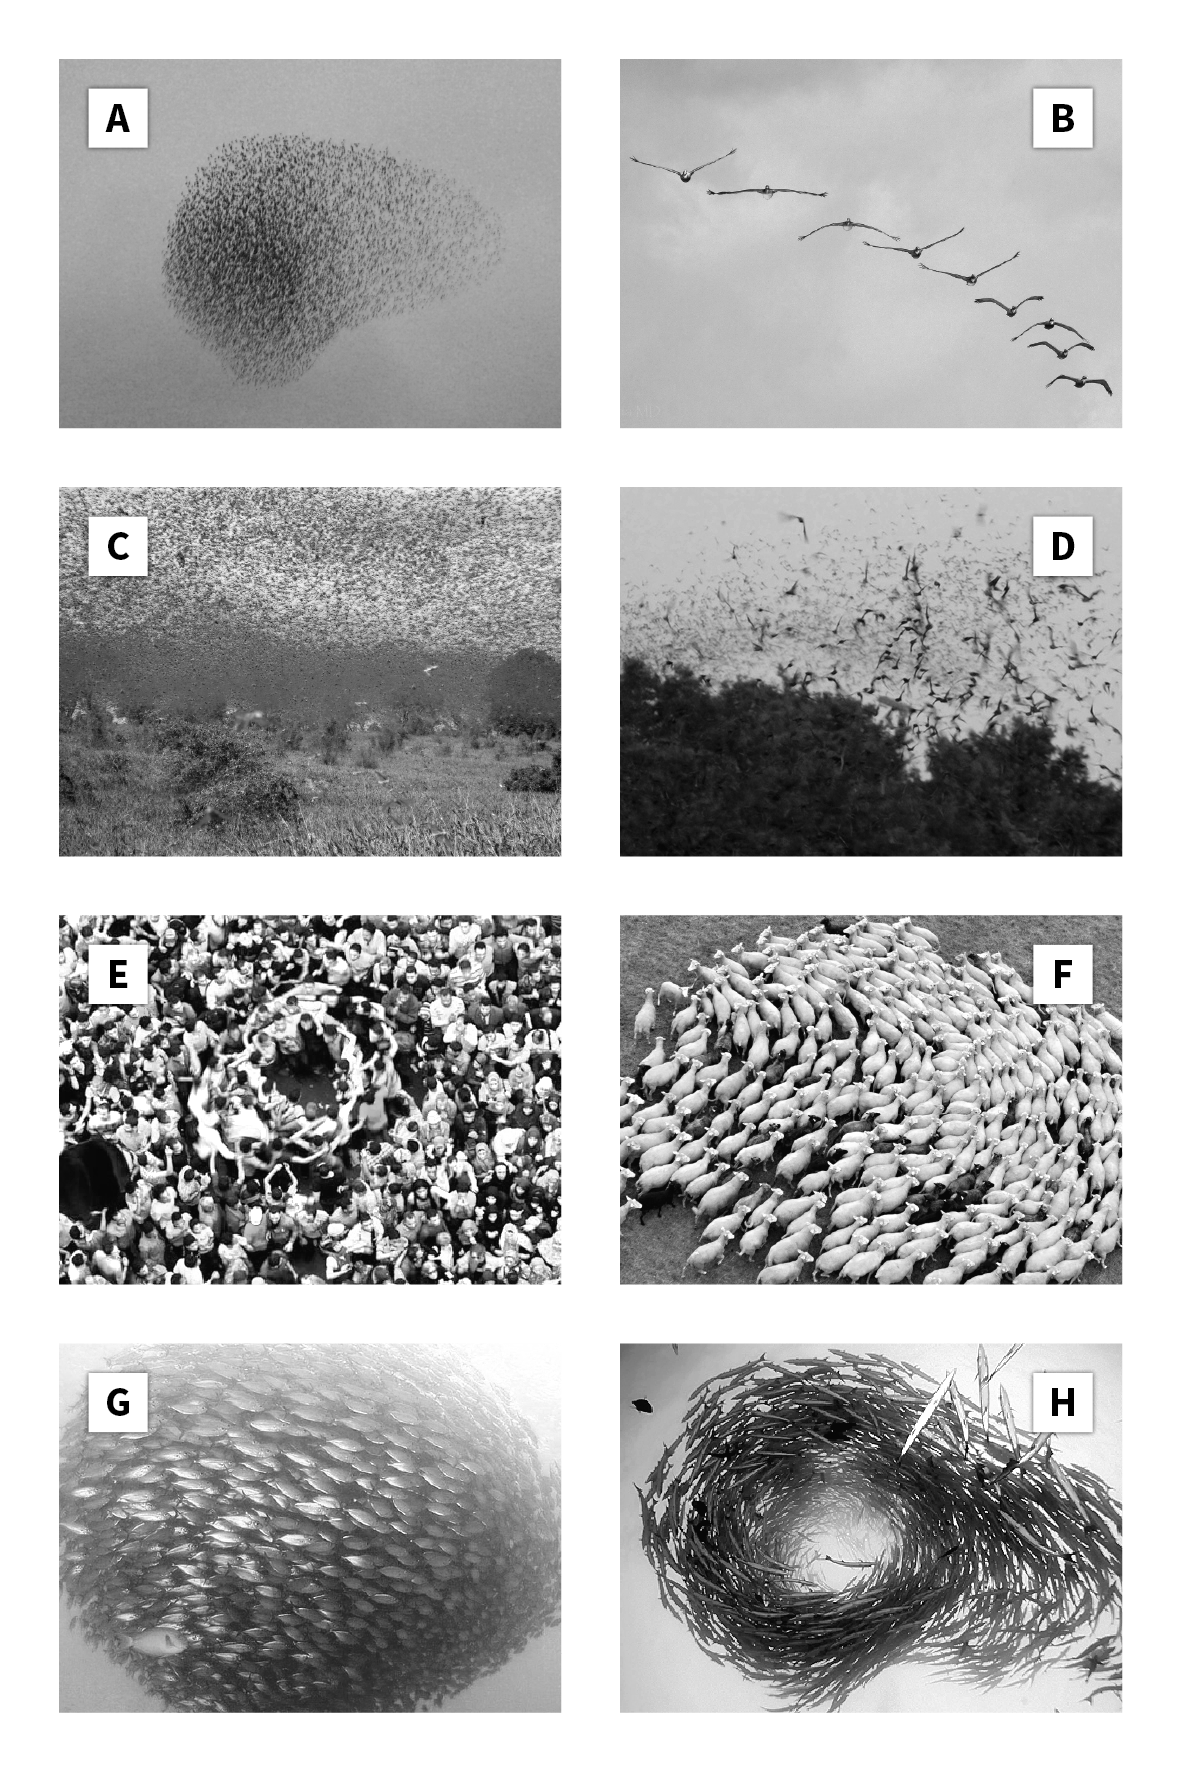
\includegraphics[width=\figurewidth]{figCB_BW}
	\caption{Examples of various forms of collective behaviour found in nature. A) a murmuration of stralings (© Tim Regan, \href{http://www.flickr.com}{flickr.com}). B) a squadron of pelicans flying in formation (© Daniel D'Auria, \href{http://www.flickr.com}{flickr.com}). C) a swarm of locusts (© FAO emergencies, \href{http://www.flickr.com}{flickr.com}). D) a swarm of bats (© Amanda, \href{http://www.flickr.com}{flickr.com}). E) a mosh pit on a rock concert (© Amanda Mustard, \href{http://www.amandamustard.com/}{amandamustard.com}). F) a herd of sheep (© Dariusz Paciorek, \href{http://www.aeroart.com.pl/}{aeroart.com.pl}). G) the bait ball phenomenon (© Bo Pardau, \href{http://www.flickr.com}{flickr.com}). H) milling fish (© Robin Hughes, \href{http://www.flickr.com}{flickr.com}).}
	\label{fig:CB}
\end{figure}

The collective behaviour research field (in certain research communities known also by the names collective animal behaviour or swarm behaviour) is very active as even though the phenomenon can be easily observed in nature, many scientific questions remain unanswered \cite{krause2002living,lebarbajec2009organized,sumpter2006principles}. In the biological community examples of such questions are why groups, especially organized ones, form in the first place, and why we see so much variation in behaviour \cite{lebarbajec2009organized}. For example, why do so few bird species that fly together display organized behaviour, and why do even closely related species \cite{jarvis2014wholegenome} display major differences in flocking behaviour \cite{lebarbajec2009organized}? The literature about collective behaviour contains several different and sometimes contradictory hypotheses about why animals coalesce into groups. Some studies advocate that aggregations boost mating and foraging efficiency \cite{krebs1994behavioural}, others claim that fish and birds in highly organized groups save energy because of hydrodynamic or aerodynamic benefits \cite{hemelrijk2014increased,marras2015fish,portugal2014upwash}.

Probably the most common hypotheses about the origins of collective behaviour state that grouping functions as an effective defence against predators \cite{cresswell2011predicting,hart2005predator,krause2002living,larsson2012why,lebarbajec2009organized,nishimura2002predator,pavlov2000patterns}. The \emph{selfish herd} hypothesis \cite{hamilton1971geometry} suggests that animals form groups in order to reduce their domain of danger -- an area surrounding an individual in which all points within that area are closer to the observed individual than to any other \cite{viscido2001response}. The \emph{dilution of risk} hypothesis suggests that the chance of a single prey being selected as the predator's target is lower in larger groups \cite{tosh2011conditions}. The \emph{many eyes} hypothesis suggests that as the size of the group increases the probability of detecting a predator also increases \cite{galton1871gregariousness} and the amount of time individuals in the group need to be vigilant against predators decreases \cite{elgar1989predator,haley2014exploring,ruxton2008application,sadedin1998influence}, giving them more time for other tasks (\eg foraging). Last but not least, the \emph{confusion hypothesis} states that a predator attacking a group of visually similar prey might have a hard time tracking and capturing its target \cite{demsar2015simulating,kunz2006prey,nishimura2002predator,olson2013predator,olson2016evolution,zheng2005behavior}.

Some manifestations of collective behaviour (\eg schools of fish and flocks of birds) are quite large in scale and as such hard to enclose in a controlled environment in which scientists could then test the hypotheses about the ``whys'' and ``hows'' of such behaviour \cite{lebarbajec2009organized}. In addition in nature different predators with different hunting tactics exist in different environments, meaning that it is difficult to compare the effects of predation pressures on the behaviour without the confounding effects of environmental context. With computational approaches one can develop models that reproduce the studied behaviour and at the same time diminish the confounding effects of the environment. It comes as no surprise then that computational approaches are a more and more frequently used tool for studying various hypotheses concerning collective behaviour \cite{vicsek1995novel,couzin2002collective,hildenbrandt2010selforganized}. Because computational approaches give scientists full control over the involved parameters, the results are usually also not species specific but more general.

%-----
\section{Individual-based models}

There are two prominent computational approaches suitable for studying collective behaviour. The first one is called Eulerian modelling, which typically uses partial differential equations to describe the flux of a property -- how that property changes through time and space. In the case of collective behaviour studies the property in question is usually population density \cite{kunz2011implications}. However, Eulerian modelling has two weaknesses, the individual variations (\eg in speed, body size, vision, etc.) cannot be easily incorporated \cite{gautrais2008keybehavioural}, and it does not allow to trace the properties on the group level back to the behaviour of individuals \cite{deangelis2005individualbased}. Eulerian modelling can thus be interpreted as a top-down approach to modelling collective behaviour, where one single equation is sought, an equation which describes the dynamics of the property in question on a global level. Needless to say, Eulerian modelling is suitable for tackling with research questions related to the global properties of collective behaviour assuming that one exists; questions related to how or why such behaviour emerges, on the other hand, are extremely difficult or impossible to answer.

Because of these reasons the most common computational approach to the study of collective behaviour is the so called individual-based modelling (also known as Lagrangian modelling, or agent-based modelling). The reasoning behind such modelling is that to be able to address questions related to how or why collective behaviour emerges the focus should be on the individual, and thus the approach can be viewed also as a bottom-up approach to modelling collective behaviour. In individual-based models the behaviour of each individual is defined by its local algorithm (local program). A local algorithm describes how an individual reacts to its neighbours, nearby environment, and possibly its own internal state. Once researches define the behaviour (reactions) of individuals they run computer simulations where many of these individuals reside in a shared environment. In these simulations, the behaviour of individuals results from local interactions and is usually calculated in turn for each individual and integrated over time. During simulations researchers observe and try to explain the patterns that emerge on a group level via local interactions \cite{grimm1999tenyears}. In other words, researchers program the behaviour of individuals (local level) and then observe the behaviour at the global level that emerges from interactions at the local level \cite{dewolf2005emergence}. In individual-based models there is usually no central or external mechanism that would impose order and structure on the global level. The emergence of order and structure from local interactions on the global level is also known as \emph{self-organization}. Self-organization is a very interesting research topic on its own as besides biological systems (\eg animal aggregations) it exists also in the world of physics (\eg Rayleigh-B{\'e}nard convection cells \cite{getling1998rayleigh}) and chemistry (\eg Belousov–Zhabotinsky reaction \cite{zhabotinsky1964periodic}). An interesting, but rather unconventional approach used for the study of self-organizing patterns is \emph{amorphous computing} \cite{abelson1996amorphous,abelson2000amorphous}, which builds computational systems made from very large numbers of identical, parallel processors each having limited computational ability and local interactions. For example, Coore \cite{coore1994botanical} demonstrated that local entities in amorphous computing can be configured to generate pre-specified patterns that resemble self-organization.

In biological studies devoted to answering questions why or how collective behaviour emerges, most often the individual-based models for simulating the motion of groups of animals are designed by hand. In such hand-crafted, or pre-set, models the behaviour of artificial animals, or \emph{animats} \cite{cliff1993adding,fine2013unifying,lebarbajec2005fuzzy,watts1998animats,wilson1985knowledge}, is designed by the researchers/programmers and then fine-tuned to as closely as possible mimic the behaviour of animals in nature \cite{couzin2002collective,demsar2014simulated,demsar2015simulating,lebarbajec2005fuzzy,lebarbajec2005simulating,hildenbrandt2010selforganized,vicsek1995novel}. When fine-tunning and validating the researchers resort to various metrics by which they compare the behaviour of animats to the behaviour of the modelled animals. The developed models (designed and fine-tuned) are then used to study the behaviour of animals by simulating various situations in a controlled environment and observing the reactions and interactions of large numbers of animats.

%-----
\section{The animat}

The animat can be defined as a Moore automaton \cite{kohavi1978switching} with a three stage transition function (see Definition~\ref{def:animat} and \figurename~\ref{fig:animat}) \cite{lebarbajec2003boids,lebarbajec2003fuzzifying,lebarbajec2005fuzzy,lebarbajec2007boids}. It abstracts the basic characteristics of a real animal. Just like a real animal, it exists in time and space and is surrounded by inanimate and animate objects (\ie the \emph{universe}). It is aware of its current state and capable of \emph{perceiving} the state of the universe. By performing \emph{actions}, governed by its \emph{drives}, the animat is capable of influencing its own state and the state of the universe \cite{lebarbajec2005fuzzy}.

\begin{definition}
	\label{def:animat}
	An animat $\autom{A}=\langle\set{X},\set{Q},\set{Y},\delta,\lambda,P,D,S\rangle$ is an extended Moore automaton, where $\set{X}$, $\set{Q}$ and $\set{Y}$ are non-empty sets representing the input alphabet, the internal states and the output alphabet respectively; $\delta: \set{X}\times \set{Q}\rightarrow \set{Q}$ is a mapping called the transition function and $\lambda: \set{Q}\rightarrow \set{Y}$ is a mapping called the output function. At any discrete time step $t \in \set{T}$, where $\set{T}$ is a non-empty set of discrete time steps, the automaton is in a state $q_t \in \set{Q}$. The state determines the future input-output behaviour. If an input $x_t \in \set{X}$ is applied, then, in the next discrete time step $t+1$, the automaton assumes a new state $q_{t+1} = \delta(x_t,q_t)$ that depends both on the current state and the input. In addition, the automaton emits the output $\lambda(q_{t+1}) \in \set{Y}$, which depends on the new state.	
	In the case of the animat its input in a given discrete time step is the perceived state of the universe (a collection of animats) at the same time step and for that reason its input alphabet is $\set{X}=\set{Y}_1 \times \cdots \times \set{Y}_n$, where $\set{Y}_1,\ldots,\set{Y}_n$ are output alphabets of the $n$ animats that represent the universe. In addition $P=\langle P_1,\ldots,P_k\rangle$, $D=\langle D_1,\ldots,D_l\rangle$, and $S$ are a $k$-tuple of perception functions, an $l$-tuple of drive functions, and an action selection function respectively and the transition function $\delta$ is defined as:
	\begin{eqnarray}
		& p_i = P_i(x,q),\ i=1,\ldots,k, & \\
		& a_j = D_j(\langle p_1,...,p_k\rangle,q),\ j=1,\ldots,l, & \\
		& \delta(x,q) = S(\langle a_1,...,a_l\rangle,q). &
	\end{eqnarray}
\end{definition}

\begin{figure}
	\vskip.2in % add some top and bottom whitespace
	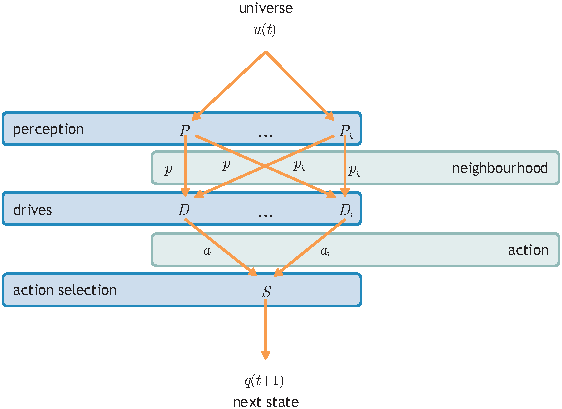
\includegraphics[width=.6\figurewidth]{fig[animat]}
	\vskip.2in
	\caption{A visual representation of the processes and terminology associated with an artificial animal, the animat.}
	\label{fig:animat}
\end{figure}

As animals in nature are able to monitor their surroundings via their senses (sight, lateral line, hearing, etc.), animats are able to perceive their \emph{neighbourhood}, the current state of the universe nearby. Animats continuously attempt to optimise the rate of occurrences of events that will fulfil their drives. Drives in animats thus imitate the instinctive needs that make real animals tick and perform actions that are necessary to survive in their natural habitat. A few examples of such drives are: the drive to feed, the drive to mate, social drives, etc. More often than not there is no ``one action to rule them all,'' meaning that there is no single action that could satisfy all of the animat's drives at the same time. For example, let us consider a hungry animal with a feeding area nearby. If there are no predators roaming around the feeding area, the decision of the animal (action selection) is trivial -- move towards the food. If there are predators nearby, however, the animal's decision becomes a bit more complicated as it has to meld the actions that will satisfy the drive to feed with those that will satisfy the drive to flee. If the animal is facing the threat of dying by starvation it might decide to move towards the food despite the danger of being eaten by a predator. On the other hand, if it is just slightly hungry it might decide that a better option would be to try and find a different source of food, a source of food that does not have predators lurking around. Therefore, the animat has to perform some kind of \emph{action selection} in order to appease its drives. In other words the action selection tries to satisfy as many of the animat's drives as posible given the animat's current state and the state of the universe nearby.

With individual-based models it has been demonstrated that complex collective behaviour can emerge if individuals follow relatively simple drives. The first attempts at modelling collective behaviour via individual-based models were made in the 1980s. Aoki \cite{aoki1982simulation} proposed a bottom-up approach to the simulation of schooling mechanisms in fish. Reynolds \cite{reynolds1987flocks} presented the first computer model for procedural animation of flocking birds. Heppner \& Grenander \cite{heppner1990stochastic}, working on a similar project, modelled the behaviour of birds with stochastic non-linear differential equations. These and subsequent individual-based models \cite{couzin2002collective,demsar2013family,demsar2014simulated,demsar2015simulating,demsar2016balanced,demsar2017evolution,helbing1995social,hildenbrandt2010selforganized,lebarbajec2009organized,parrish2002schools,schellinck2011review,sumpter2006principles,vicsek2012collective} differ in the way they implement individual parts, but in most models the behaviour is a constant blending of three drives called \emph{cohesion}, \emph{separation}, and \emph{alignment} (see \figurename~\ref{fig:drives}). Cohesion denotes the attraction toward other individuals and is usually modelled as the tendency to move towards distant individuals when there are none nearby; separation models the tendency to move away from neighbours that are too close, to avoid collisions. The third drive, alignment, models the tendency to synchronize velocity (direction and speed of movement) with nearby neighbours. As a perfect synchronization of movements will prevent collisions and lead to the formation of groups the alignment drive can be interpreted also as a passive form of avoidance and attraction, and due to this some models concentrate exclusively on the alignment drive \cite{vicsek1995novel}.

\begin{figure*}
	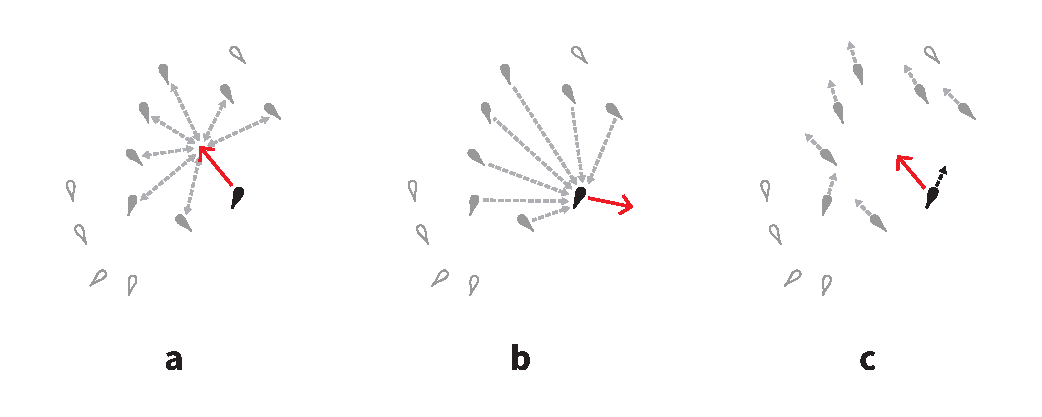
\includegraphics[width=\linewidth-7pt]{figDrives}
	\caption{Visualization of the three basic drives: (a) cohesion, (b) separation, and (c) alignment. The black animat is the observed individual. The grey animats are the perceived neighbours that influence the observed animat's behaviour. The white and outlined animats are neighbours that have no direct influence on the observed animat's behaviour.}
	\label{fig:drives}
\end{figure*}

%-----
\section{Evolvable animats}

An alternative approach to hand-crafted models is to design a system in which animats can adapt to the environment by tweaking the parameters that define their own behaviour. The animats change their behaviour to satisfy their drives in a more efficient way. Traditionally this is achieved through the application of genetic algorithms -- algorithms that by means of \emph{selection}, \emph{crossover}, and \emph{mutation} imitate natural evolution for finding solutions to various problems \cite{goldberg1989genetic,goldberg2002design,holland1992adaptation}. Here, every potential solution to the problem that is being solved is represented by its own chromosome. Selection mimics the survival of the fittest principle in nature, where the best specimens of a certain species have a higher probability of reproductive success than the weak ones, thus stronger individuals will leave the most copies of their genetic material in successive generations. Crossover emulates the exchange of genetic material during reproduction. When two parents produce an offspring their chromosomes are recombined to form the chromosome of the child and in the process the traits of parents are transfered to the child. As in nature the anomalies in the process may result in insertion or deletion of genetic information into the child's chromosome, genetic algorithms in their last operation perform mutation, where on rare occasions parts of the child's chromosome will randomly change.

In most applications of genetic algorithms the generational boundaries are clearly defined. In every generation the whole population of potential solutions to the problem that is being solved (chromosomes) is evaluated via simulation to extrapolate the fitness (assess the quality) of every individual solution. The fitness is then used for selection, followed by crossover and mutation so that the whole population of possible solutions (chromosomes) is created anew and is defined as a new generation.

In recent years a number of hi-impact studies \cite{kunz2006prey,olson2013predator,olson2016evolution,biswas2014causes,demsar2015simulating,demsar2016balanced,demsar2017evolution,hein2015evolution} used genetic algorithms to gain new insight into how external pressures shape the behaviour of animals and what type of external pressures promote the evolution of collective behaviour. A number of researchers evolved only various parameters required for the implementation of drives by means of differential equations \cite{sayers2009evolved,spector2003emergence,wood2007evolving}. The main issue of this approach is that using known and predefined drives will most likely steer the evolution towards known forms of collective behaviour. Reynolds \cite{reynolds1993evolved} was the first to use genetic algorithms \cite{holland1992adaptation} in combination with genetic programming \cite{koza1992genetic} to attempt the evolution of collective behaviour without predefined drives. The simple behaviour that emerged, however, cannot be compared to the complexity of collective behaviour that can be observed in nature, mainly because Reynolds made too many simplifications. Zaera\etal \cite{zaera1996not} attempted to evolve fish schooling with artificial neural networks and genetic algorithms, but they did not succeed in completing the task at hand. They suggest that the main reason for failure was in the fitness function as it is hard to define the perfect one because it is hard to measure collective behaviour on the global level from the point of view of an individual. Indeed, the fitness function is the key element of genetic algorithms; it determines which solutions will continue the process of evolution and which will die out.

Assessing collective behaviour from the point of view of an individual is problematic from at least two perspectives. First, the definition of the degree of collective behaviour is not clear. There are several different forms of collective behaviour in nature, each one spectacular and beautiful in its own way. And second, assessing the degree of collective behaviour from the point of view of an individual for the purpose of evaluating its fitness explicitly defines the direction of evolution; individuals are steered into finding actions that will lead to an increase of the degree of collective behaviour. While this might be non problematic in traditional use of genetic algorithms (finding near-optimal solutions to difficult problems), it becomes problematic when one wants to investigate the reasons that might have led to the emergence of collective behaviour, \ie when one wants to answer questions such as why or how collective behaviour emerges. For such questions one should instead be interested if animats will resort to collective behaviour as a result of natural evolution, without an explicit fitness function -- an approach typical for investigations in the field of Artificial life. As a matter of fact, a number of studies \cite{biswas2014causes,hein2015evolution,olson2013predator,olson2015exploring,olson2016evolution,witkowski2016emergence} successfully overcame the issue by using a more subtle fitness function. In these studies fitness was assesed through the ability of individuals to survive in various hostile artificial environments. The actions required to survive were similar to those that living animals perform in nature -- avoid predators, search for food, etc. The animats that were successful at surviving had more opportunities and a higher probability of reproducing. With this they had a higher chance of spreading their genetic material. And since offspring inherit the traits of parents, they were also traditionally more successful at staying alive. Collective behaviour emerged if and only if it had a positive effect on prey survivability. However, the collective behavior that emerged can in most cases \cite{biswas2014causes,hein2015evolution,olson2013predator,olson2015exploring,olson2016evolution,witkowski2016emergence} be classified into two forms -- clumping and swarming. None of these studies succeeded in producing the highly organized forms of collective behaviour that we admire in flocks of birds and schools of fish, namely their dynamic parallel motion and/or milling \cite{couzin2002collective,sumpter2006principles}. And this is what we aimed to achieve in this thesis.

%-----
\section{The fuzzy animat}

The two most common approaches for implementing animats adopt either differential equations \cite{couzin2002collective,hildenbrandt2010selforganized,reynolds1987flocks,vicsek2012collective} or artificial neural networks \cite{kunz2006prey,witkowski2016emergence,zaera1996not}. Artificial neural networks \cite{mcculloch1943logical} are universal and highly flexible function approximators that loosely model the behaviour of neural units in human brains. Even though these two approaches gave us a tremendous amount of new insight into the fascinating field of collective behaviour, they have some drawbacks that are potentially problematic for future advances. The two main problems of differential equations are that the exact values of several parameters in the equations are often unknown, and that researchers usually need solid mathematical knowledge to modify and tune the behaviour of animats. The main issue of artificial neural networks is that the models based on them are usually hard to interpret and understand from a human point of view. This is why artificial neural networks are sometimes labelled as the ``black box'' approach \cite{paruelo1997prediction,lek1999artificial,ozesmi1999artificial}. 

Lebar Bajec\etal \cite{lebarbajec2005fuzzy,lebarbajec2005simulating} suggested that the above and some other pitfalls may be alleviated by using fuzzy logic \cite{zadeh1965fuzzy}. Just like artificial neural networks, fuzzy logic is a universal and highly flexible function approximator. One of the main advantages of fuzzy logic is its power when dealing with ambiguous (uncertain, vague, etc.) or unknown parameters of the models. Another advantage of fuzzy logic based modelling is that fuzzy models are described with linguistic rules similar to sentences that humans use for communication on a daily basis \cite{kosko1994fuzzy,lebarbajec2005fuzzy,lebarbajec2005simulating,mamdani1974application,mamdani1975experiment,mendel2001uncertain,zadeh1965fuzzy}. The idea that with fuzzy logic one can transform the on-field observations made by biologists into computer models with relative ease has been supported by numerous studies \cite{dasilva2008predator,demsar2013family,demsar2014simulated,demsar2016balanced,demsar2017evolution,gras2009individualbasedevolving,lebarbajec2005fuzzy,lebarbajec2005simulating,mashayekhi2015individualbased,tron2004mathematical}.

Indeed, starting from this idea Lebar Bajec\etal in 2005 defined the \emph{fuzzy animat} \cite{lebarbajec2005fuzzy,lebarbajec2005simulating}, an artificial animal based on fuzzy logic. From the formal standpoint the main difference between the classic animat and the fuzzy animat is in the approach used to implement the animat's transition function. In the case of a fuzzy animat fuzzy logic can be used for the description of perception functions, drive functions, and the action selection function (see Definition~\ref{def:animat}). Most often \cite{lebarbajec2003boids,lebarbajec2003fuzzifying,lebarbajec2005fuzzy,lebarbajec2005simulating,lebarbajec2007boids,moskon2007fuzzy} the biggest difference is probably in terms of drives; in the case of the classic animat the drives are usually implemented with differential equations while in the case of the fuzzy animat the drives are implemented as \emph{fuzzy rule-based systems}.

A fuzzy rule-based system is defined through a so called \emph{fuzzy knowledge base}, which consists of two components: a \emph{fuzzy data base} and a \emph{fuzzy rule base} \cite{herrera1996genetic}. The data base declares the fuzzy variables, the linguistic terms, and the interpretation of logic connectives, while the rule base uses a collection of if-then rules (a linguistic description) to describe the system's behaviour. An example of a simple fuzzy knowledge base of a fuzzy rule-based system used for a room temperature controller is presented in \figurename~\ref{fig:knowledgebase}.

\begin{figure}
	\vskip.25in % add top and bottom whitespace so that the caption does not overflow the figure box
	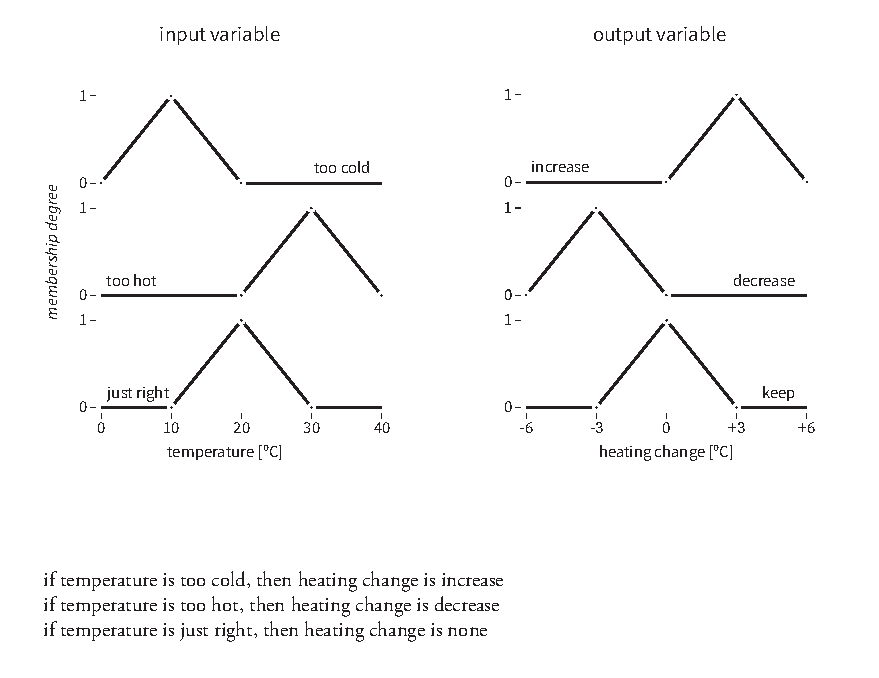
\includegraphics[width=\figurewidth]{figKnowledgebase}
	\vskip.25in
	\caption{An example of a simple fuzzy knowledge base. It describes a fuzzy rule-based system of a room temperature controller. The top part is a visual representation of the fuzzy data base. It defines two fuzzy variables, one input and one output. The input variable is the current room temperature, which is mesaured by the system via a temperature sensor. The rule base (bottom part) describes how input variables are translated into actions (output variables) via fuzzy if-then rules. In our case the action of the temperature controller is a change in room heating.}
	\label{fig:knowledgebase}
\end{figure}

In the case of animats the fuzzy data base describes how they perceive and interpret their neighbourhood and what actions they can execute to change their state and consequently the state of the universe. As such, the fuzzy data base defines the interpretation of various data obtained by the fuzzy animat's sensory system (\eg the distance to the nearest neighbour animat, heading direction of the predator animat, position of obstacles, etc.), and the actions availabe to the animat (\eg speed change, heading change, etc.). How the fuzzy animat translates the available information into actions is then defined with the fuzzy rule base.

%-----
\section{Goal: evolvable fuzzy animats}

The main goal we set ourselves for this thesis was to develop an evolutionary model, based around fuzzy logic, suitable for simulating evolution of collective behaviour inside an artificial world. As the most common hypothesis about the origins of collective behaviour states that collective behaviour might have evolved as a protection from predators \cite{cresswell2011predicting,hart2005predator,krause2002living,larsson2012why,lebarbajec2009organized,nishimura2002predator,pavlov2000patterns} it is to be expected that the direct competition between predators and prey should most likely be part of an evolutionary model that wishes to study the origins of collective behaviour. In order to properly design the model, and later evaluate it, we, for this reason, first studied the predator-prey relation and interactions in a hand-crafted model. By analysing the target selection (predation) tactics in a hand-crafted model we gained important insight into the complex world of predation tactics and prey responses to attacks. During this process we also discovered that existing models most often use basic predation tactics, whereas predators in nature adopt quite advanced approaches when hunting prey. Thus we next developed an evolutionary model where predators can tune their hand-crafted predation tactics to increase their hunting success, which could potentially give us the answer to what predation tactic is optimal for certain forms of collective behaviour or prey responses.

By using the results obtained by these two studies \cite{demsar2014simulated,demsar2015simulating} we then designed a \emph{genetic fuzzy system} for the simulation of evolution of collective behaviour. Genetic fuzzy systems \cite{cordon2001genetic,cordon2004ten,fernandez2015revisiting,herrera1996genetic,herrera2008genetic,pedrycz1996fuzzy,sanchez1997genetic} use genetic algorithms for optimizing existing or constructing new knowledge bases of fuzzy rule-based systems. Most genetic fuzzy systems focus on the optimization of hand-crafted fuzzy systems \cite{cordon2004ten,fernandez2015revisiting,herrera2008genetic}. A more demanding approach is \emph{genetic learning of fuzzy systems}, where components of a fuzzy system (the rule base, the data base, or the entire knowledge base) are not only tuned but constructed via genetic algorithms.

There are two prominent approaches for genetic rule learning -- the Michigan \cite{holland1977cognitive}, and the Pittsburgh \cite{smith1980learning} approach. With the Michigan the chromosome, as defined by the genetic algorithm, represents an individual rule and a rule base is presented by the entire population of chromosomes in a generation. The quality of the rule base (its capability of solving the problem at hand) therefore progresses through clearly defined generations. As this would lead to all animats having the same rule base we opted to use the Pittsburgh approach. With it the chromosome represents an entire rule base. This allowed us to interpret each animat individually (defined by a single chromosome) and move away from the traditional use of genetic algorithms with clear generational boundaries and closer to artificial life where there is no clear generational boundary (selection, crossover and mutation are simply part of evolution). As each animat is defined through its own chromosome, this also means that the population of animats is heterogeneous (if not by physiology by behaviour at least). This also means that the differences in individual chromosomes (rule bases) represent a source of indirect competition in the model (via their rule bases the animats compete for survival in the artificial world). One could say that prey animats in our model have to survive in an environment that is competitive in two ways. First, prey animats compete with predators for survival, and second they compete with each other to have a higher chance for reproduciton. With this and the consideration of various predation tactics we managed to design an evolutionary system that is capable of generating a wider repertoire of collective behaviours than previous approaches \cite{biswas2014causes,hein2015evolution,olson2013predator,olson2015exploring,olson2016evolution,reynolds1993evolved,sayers2009evolved,spector2003emergence,wood2007evolving}.

%-----
\section{Research methodology}

\begin{figure}
	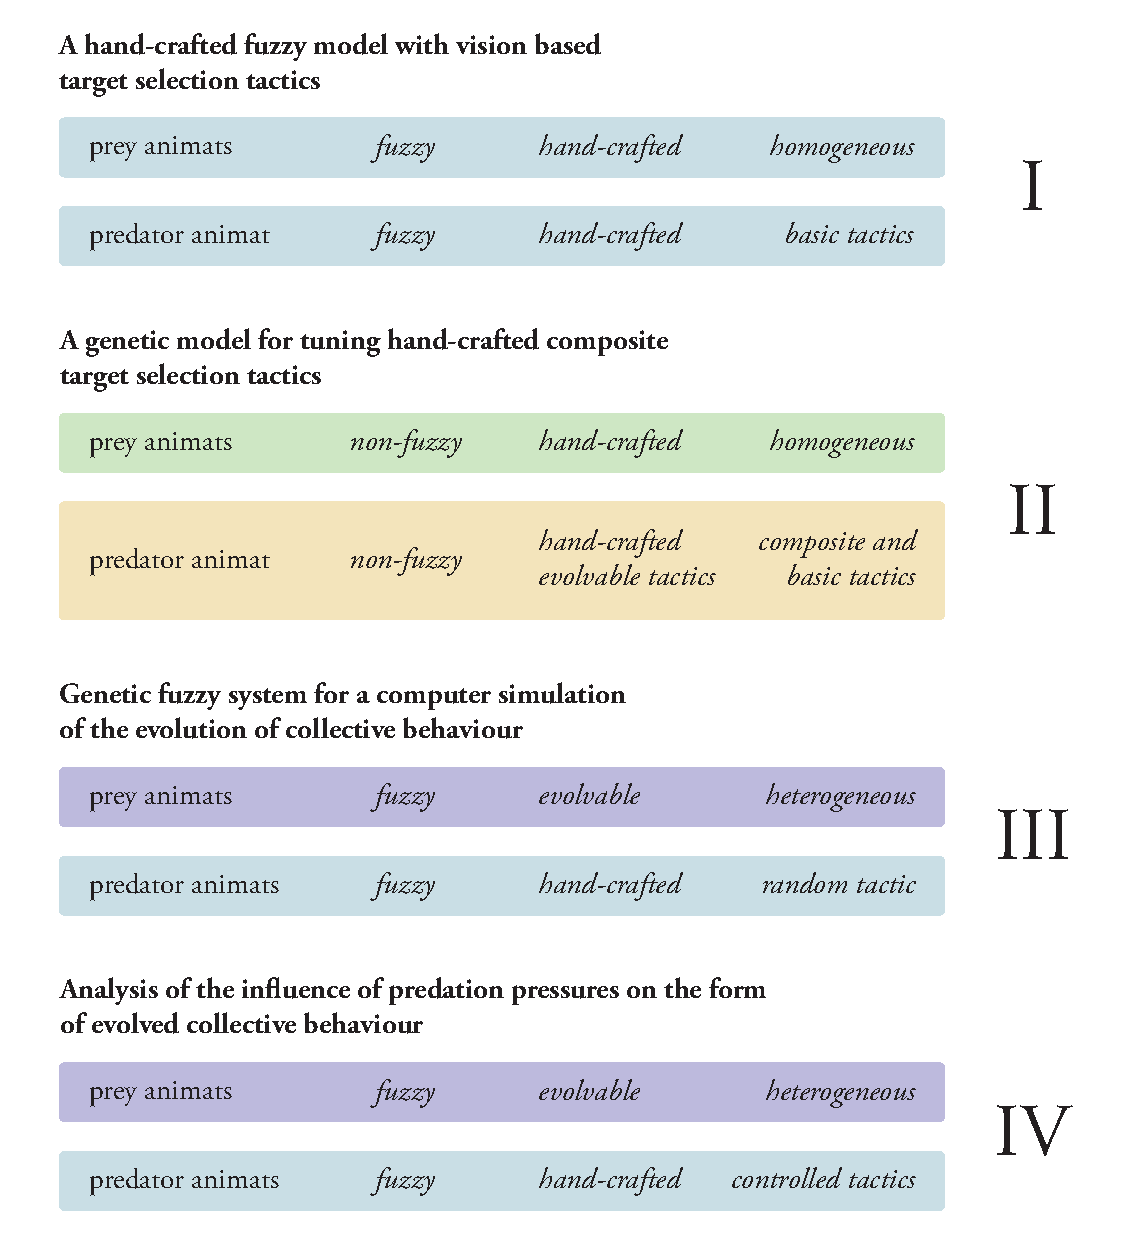
\includegraphics[width=\figurewidth]{stages2}
	\caption{A visual representation of models used in all four stages of this thesis.}
	\label{fig:stages}
\end{figure}

We split our research into four stages, each with a specific sub-goal. During these stages we developed three different individual-based models. \figurename~\ref{fig:stages} visualizes the four sub-goals and the main differences between the models used for achieving these sub-goals.

In the first model we upgraded an existing fuzzy model for computer simulation of bird flocking \cite{lebarbajec2005fuzzy,lebarbajec2005simulating}. Our principal contributions were a) the design of a perception function which mimics vision and takes into account limitations in cognitive capabilities, and b) introduction of a predator animat. The behaviour of both types of animats (the predator and prey animats) was hand-crafted. The introduction of the predator animat necessitated also the revision of the prey animats with additional drives. The behaviour of prey animats was thus based on five drives: cohesion, separation, alignment, regulate speed, and hide (escape). Cohesion, separation and alignment are visualized in \figurename~\ref{fig:drives}. The regulate speed drive implements the tendency to move with an optimal speed if there is no predator nearby. The hide drive, on the other hand, implements the tendency to escape from predators. As the behaviour of all prey animats was governed by exactly the same drives and there was no variability in their parameters prey groups were homogeneous. The behaviour of the predator was governed only by the seek (hunt) drive. A drive which implemented the tendency of predators to chase their targeted prey individual. For further details of the model refer to Chapter \ref{chap:alife}. The model was used to investigate the general hypothesis that grouping may serve as a protection from predation.

In the second stage we developed an individual-based model where the drives are implemented via differential equations (non-fuzzy). This was done to achieve comparability with previous similar models and to keep computational complexity as low as possible. The drives for both types of animats (predator and prey) were hand-crafted. In the case of prey animats the behaviour was based on previous zone-based models \cite{aoki1982simulation,couzin2002collective} and governed by the cohesion, separation, alignment and escape drive. Prey groups were homogeneous -- there was no variability in neither drives nor parameters of prey animats. The behaviour of the predator was governed only by the hunt drive. The model was used to study the evolution of composite predation tactics. To do so the parameters of each tactic were tuned with genetic algorithms, meaning that a predator was able to adapt its target selection tactic in order to increase its hunting success. See Chapter \ref{chap:ecomod} for further details of the model. 

The research in the third and fourth stage was conducted with the same individual-bsaed model, an artificial life-like genetic fuzzy system suitable for simulating the evolution of prey behaviour. The only difference was that in the third stage predators used random predation tactics while in the fourth stage the predation tactics were carefully picked to put certain evolutionary pressures on prey. Both types of animats (predators and prey) were modelled with fuzzy logic. The behaviour of predators was hand-crafted and very similar as in the first stage of our research. Predators only had one drive, the hunt drive, which implements their tendency to chase the targeted prey individual. In contrast to stage two, the predators did not adapt their behaviour through evolution. The behaviour of prey animats, on the other hand, evolved through time. Evolution of prey animats in the third and fourth stage was performed via genetic rule learning (construction of fuzzy rule bases with genetic algorithms). As we used the Pittsburgh approach for genetic rule learning each prey animat was governed by its own set of rules and could behave differently from all the other prey animats. This in turn means that prey groups were heterogeneous See Chapters \ref{chap:plos} and \ref{chap:scirep} for further details of the model. In the third stage we investigated if the model is capable of evolving a wider repertoire of collective behaviours than previous approaches, and in the fourth stage we investigated what predation pressures lead to the emergence of specific forms of collective behaviour.

%-----
\section{Scientific contributions}

We started this research with two goals in mind. The first goal was an analysis of how predator strategy and prey grouping (\eg bird flocking, fish schooling, etc.) influence prey survivability. Research devoted to achieving this gaol resulted in two scientific contributions, listed at the end of this section as a) \emph{A hand-crafted fuzzy model with vision based target selection tactics} and b) \emph{A genetic model for tuning hand-crafted composite target selection tactics} at the end of this section. Each contribution was presented on its own in the form of an original scientific paper in a renowned scientific journal. The manuscripts are included in this thesis in their entirety as Chapters \ref{chap:alife} and \ref{chap:ecomod}.

The second goal was the development of a co-evolutionary genetic fuzzy system suitable for simulating the evolution of collective behaviour. While we were working on our first goal Olson\etal \cite{olson2013critical,olson2013predator,olson2016evolution} developed a model similar to the one we set to develop as part of our second goal. They designed a probabilistic version of the animat based on Markov Networks and simulated co-evolution of predators and prey that lived in a shared environment. Results from these studies suggest that prey individuals in their case always evolved a swarming behaviour. In nature, however, collective behaviour can be observed in many forms –- swarming, milling, dynamic polarized motion, etc. Other existing evolutionary models \cite{biswas2014causes,hein2015evolution,olson2013predator,olson2015exploring,olson2016evolution,reynolds1993evolved,sayers2009evolved,spector2003emergence,wood2007evolving} were aslo unable to reproduce such a wide repertoire of collective behaviours. We view this gap between the forms of collective behaviour that can be observed in nature and those evolved via artificial evolution as the major weakness of current evolutionary models. For this reason, we decided that in lieu of focusing on co-evolution of predators and prey we will focus on designing a genetic fuzzy system capable of evolving a wider repertoire of collective behaviours. The co-evolution of predators and prey usually leads to a continuous co-adaptation of predator and prey behaviours. Needless to say such an analysis although interesting would be extremely time consuming. Thus, for reasons of simplicity the predator animat in our model is hand-crafted, \ie excluded from evolution, only prey animats co-evolve through time. Their co-evolution is the result of their direct competition with predators for survival, them being heterogeneous in behaviour, and their indirect competition where they compete with each other to have a higher chance of reproduction. This also allowed us to analyse the evolved behaviours in a more controlled manner. Research devoted to achieving our new gaol resulted in two scientific contributions, listed at the end of this section as a) \emph{Genetic fuzzy system for a computer simulation of the evolution of collective behaviour} and b) \emph{Analysis of the influence of predation pressures on the form of evolved collective behaviour} at the end of this section. Each contribution was presented on its own in the form of an original scientific paper in renowned scientific journal and the manuscripts are included in this thesis in their entirety as Chapters \ref{chap:plos} and \ref{chap:scirep}.

\subsection*{A hand-crafted fuzzy model with vision based target selection tactics} We started our research by expanding an existing fuzzy logic based model \cite{lebarbajec2005fuzzy,lebarbajec2005simulating} with predators and visual perception. Here we implemented three target selection tactics, all from the visual perspective of the predator (attack the nearest visible individual, attack the most visually isolated individual, and attack the centre of the visible group). This allowed us to study the influence of predation tactics and the impact of collective behaviour on survivability of prey individuals \cite{demsar2014simulated} . Our results suggest that for prey individuals social behaviour (governed by the separation, alignment, and cohesion drives) as opposed to individualistic (governed exclusively by the separation drive) is the most beneficial (predators take longer to capture their target). Predators, on the other hand, capture social prey individuals quicker when they attack the most visually isolated individual, but capture individualistic prey faster if they focus on the nearest prey individual.

\subsection*{A genetic model for tuning hand-crafted composite target selection tactics} In the next stage we developed an evolutionary model with which we studied composite target selection tactics \cite{demsar2015simulating}. For reasons of computational simplicity we here expanded on a known mathematical model of prey collective behaviour. This allowed us to concentrate on predator target selection tactics. We investigated the evolution of the optimal tactic with respect to prey behaving collectively and prey that performed a delayed response as a form of a defensive manoeuvre \cite{partridge1982structure}. Our results suggest that a composite tactic termed dispersing tactic, where the predator first dives deep into the group of prey and then targets the most peripheral individual, is the best tactic. This tactic seems to be the only tactic capable of at least partially diminishing the effectiveness of the preys' delayed response. This was a clear indication of potential interplay between target selection tactics and prey behaviour.

\subsection*{Genetic fuzzy system for a computer simulation of the evolution of collective behaviour} Armed with this knowledge, we developed an artificial life-like open-ended evolutionary model, where the behaviour of prey and predator individuals is governed by fuzzy logic \cite{demsar2017evolution}. In this model we focused on the evolution of prey behaviour when prey individuals face different predation tactics. We demonstrated that in this model prey individuals are capable of evolving a varied spectre of collective behaviours (swarming, milling, polarized motion, dynamic motion). Interestingly, the analysis of the evolved rule bases showed a statistically significant difference between different types of behaviour in the proportion of rules that take into account predator related information. This suggested that the predation pressures the prey are subject to during evolution might have a crucial influence on the behaviour that evolves.

\subsection*{Analysis of the influence of predation pressures on the form of evolved collective behaviour} The last step of our research was thus a controlled experiment where prey evolved under various predation tactics \cite{demsar2016balanced}. Here we let prey individuals evolve under four predation tactics, two of which according to previous research pressure prey to evolve dispersing and two pressure prey to evolve grouping. Our results suggest that antagonism in pressures, where prey are exposed to pressures for which the best response is both grouping and dispersing simultaneously, might be necessary for prey to evolve polarized movement.

	% !TeX root = ./thesis.tex










%==============================
\chapter{Review of published work}
\label{chap:review}

%-----
\EBlettrine{This} thesis can be divided into four separate stages. In the first two stages, \emph{Simulated predator attacks on flocks: a comparison of tactics}, and \emph{Simulating predator attacks on schools: evolving composite tactics}, we studied how various predation tactics influence the survivability of prey and what kind of adaptations by prey individuals decrease the predation success of predators. In the third stage, \emph{Evolution of collective behaviour in an artificial world using linguistic fuzzy rule-based systems}, we developed a genetic fuzzy system that is capable of simulating artificial evolution and thus generating a number of diverse forms of collective behaviour observable in nature. In the last stage, \emph{A balanced mixture of antagonistic pressures promotes the evolution of parallel movement}, we systematically investigated how various predation tactics influence the evolved behaviour of prey.

%-----
\section[Simulated predator attacks on flocks: a comparison of tactics]{Simulated predator attacks on flocks:\\ a comparison of tactics}

Starting with an existing fuzzy logic based model \cite{lebarbajec2005fuzzy,lebarbajec2005simulating} we integrated recent discoveries about vision based interaction (topologic interaction \cite{ballerini2008interaction} and occlusion \cite{kunz2012simulations}) and introduced vision based predators \cite{demsar2014simulated}. This allowed us to study the behaviour of systems that contain several types of animats including predator-prey interaction. In most individual-based models that simulated predator-prey interactions at the time of that study, predators attacked the centre of prey groups. This appears contradictory to the hypothesis that collective behaviour evolved as a protection against predators. For this reason we investigated how predator attack tactics and prey behaviour influence the survivability of prey individuals. We tuned the parameters that define the movement characteristics of animats, \eg speed and manoeuvrability, on empirical data so that the group dynamics and escape patterns were similar to those in nature.

Our results suggest that prey individuals that exhibit social behaviour (governed by the separation, alignment and cohesion drives) have a higher chance of surviving predator attacks opposed to prey individuals with individualistic behaviour (governed exclusively by the separation drive). The results support the hypothesis that grouping might function as a defensive mechanism. By implementing three target selection tactics that take into account the visual perspective of the predator (attack the nearest visible individual, attack the most visually isolated individual, and attack the centre of the visible group) we were able to provide support for this hypothesis from the predator's perspective as well. When predators attacked social prey individuals, they captured their targets faster if they attacked the most visually isolated individual, which suggest that moving in tight and evenly spaced groups might make it hard for predators to select and track their targets. When predators attacked prey with individualistic behaviour they were the most successful if they focused on the nearest prey individual. The reason might be because in the absence of social behaviour predators can reach the nearest prey individual the fastest. In nature this tactic is typically used by predators that try to minimize energy costs for prey capture.

%-----
\section[Simulating predator attacks on schools: evolving composite tactics]{Simulating predator attacks on schools:\\ evolving composite tactics}

In previous individual-based models of predator-prey interactions, including ours, predators mainly used one of several basic attack tactics; attack the centre of the group/the most central individual, attack the nearest individual, or attack the most (visually) isolated individual. In nature however, predators appear to use elaborate target selection and pursuit/hunting tactics \cite{cresswell2011predicting,forsman1998visual,gazda2005division,handegard2012dynamics,hector1986cooperative,kane2014falcons,lopez2006bottlenose,nottestad2002digging,rutz2012predator} and prey vice-versa resort to different defensive tactics (\eg grouping, grouping with a delayed response). In addition, results of our first stage of research suggested that the predator's optimal tactic depends on the prey's behaviour. This motivated us into developing an evolutionary model that tunes the parameters of hand-crafted predators \cite{demsar2015simulating}. For reasons of comparability and computational simplicity we opted to expand on an existing hand-crafted non-fuzzy prey and predator model. In the developed model predators were able to adapt their target selection tactic to diminish the effectiveness of the defensive actions of prey and increase their hunting efficiency.

Our results suggest that the basic attack tactics (attack the most peripheral prey individual, attack the nearest or attack the most central prey individual) are suboptimal, as they were all outperformed by a composite attack tactic, which we named as the \emph{dispersing tactic}. With the dispersing tactic the predators first dived deep into the centre of a nearby group of prey and then after causing chaos and dispersion of the group focused on isolated individuals. Interestingly this tactic can be commonly seen in nature when various predators, \eg swordfish (\emph{Xiphias gladius}), attack groups of prey \cite{larsson2012why,pavlov2000patterns}. In turn our results corroborate with the hypothesis that late but rapid group escape patterns commonly observed in nature \cite{partridge1982structure} help prey individuals decrease the efficiency of predators. Our results also suggest that when predators attack groups of prey that delay their escape response the dispersing tactic is again the most successful one from the predator's perspective. The dispersing tactic seems to be the only tactic capable of at least partially diminishing the effectiveness of the preys' delayed response.

During this study we also investigated the impact of the confusion hypothesis on the evolution of composite predation tactics. The confusion hypothesis suggests that prey groups work as a defensive mechanism because predators have a hard time tracking a single target in a vast group of visually similar animals. Because without consideration of predator confusion all tactics converged to similar values, our findings seem to suggest that predator confusion might have played an important role in the evolution of composite predation tactics, as well. The results of this study were a clear indication of potential interplay between target selection tactics and prey group behaviour.

%-----
\section{Evolution of collective behaviour in an artificial world\\ using linguistic fuzzy rule-based systems}

Armed with the knowledge gained in the first two stages of this research we developed an artificial life-like, open-ended, evolutionary model where competition between predators and prey in the battle for survival is the principal force that steers the evolution of prey \cite{demsar2017evolution}. In this model the behaviour of prey and predator individuals was governed by fuzzy logic. We used the model to study the evolution of prey behaviour when prey individuals are forced to live in a shared environment with various types of predators using diverse predation tactics. The predators were hand-crafted and tuned based on results from the previous stages of this research.

We demonstrated that the newly developed model is capable of producing a number of different forms of collective behaviour that both visually and quantitatively \cite{couzin2002collective,vicsek2012collective,tunstrom2013collective} resemble collective motion commonly observed in nature (swarming, milling, polarized motion, dynamic motion). Since the behaviour of every individual prey animat was described in the form of linguistic if-then rules this allowed us to study the logic behind the evolved behaviours. Interestingly, the analysis of the evolved rule bases showed a statistically significant difference between different forms of collective behaviour in the proportion of rules that take into account predator related information. This suggests that the predation pressures the prey are subject to during evolution might have an influence on the behaviour that evolves.

%-----
\section{A balanced mixture of antagonistic pressures promotes\\ the evolution of parallel movement}

Based on the indication that predation pressure might influence the form of evolved collective behaviour the last stage of research was a controlled experiment where prey evolved while subject to multiple simultaneous predation pressures. We investigated the influence of four predation tactics, two of which according to previous research pressure prey to evolve dispersing and two that pressure prey to evolve grouping. We analyzed the evolved behaviour via the prey density, polarization, and angular momentum metrics \cite{couzin2002collective,olson2016evolution,tunstrom2013collective}.

Experiments with predators to which the expected natural defensive response was either grouping or dispersing corroborate previous studies \cite{biswas2014causes,olson2013predator,olson2016evolution,wood2007evolving}. When predators pressure prey towards grouping, prey evolve behaviours that result in an increase in prey density. When they pressure prey towards dispersing, prey evolve behaviours that result in a decrease in prey density. In all of these cases prey most often resorted to collective motion similar to swarming and milling. More interesting results came from experiments where prey evolved while under threat from predators that use antagonistic predation pressures. Pressures that push prey to evolve grouping and dispersing simultaneously. Our results suggest that antagonism in pressures, where prey are exposed to pressures for which there is no clear best response (grouping or dispersing), might be necessary for prey to evolve polarized movement.


	% !TeX root = ./thesis.tex










%==============================
\chapter[Simulated predator attacks on flocks: a comparison of tactics]{Simulated\\ predator attacks on flocks:\\ a comparison of tactics}
\label{chap:alife}

\chapterAbstract[published={alife/Demsar_Lebar_Bajec_2014.pdf}, keywords={Bird, flock, artificial life, boid, fuzzy logic, predator}]{It is not exactly known why birds aggregate in coordinated flocks. The most common hypothesis proposes that the reason is protection from predators. Most of the currently developed examples of individual based predator-prey models assume predators are attracted to the centre of a highly coordinated flock. This proposed attraction of a predator to a flock would appear to be contradictory to an alternate hypothesis that flocks evolved as a protection against predation. In an attempt to resolve this apparent conflict, in this article we use a fuzzy individual based model to study three attack tactics (attack centre, attack nearest, attack isolated) and analyse the success of predation on two types of prey (social and individualistic). Our simulations revealed that social flocking (as opposed to individualistic behaviour) is the optimal anti-predatory response to predators attacking mainly isolated individuals.}

%-----
\section{Introduction}

The study of collective behaviour is a fascinating field that analyses how simple actions of an individual influence the complex global dynamics of a group. Aristotle once stated: ``The whole is greater than the sum of its parts.'' -- a statement that describes the essence of collective behaviour. Typical examples of collective behaviour are flocks of birds, schools of fish and swarms of insects; phenomena that can be easily observed in nature. Collective behaviour is also interesting because similar patterns emerge at smaller scales (cellular level) \cite{deisboeck2009collective,spector2003emergence}. Even though collective behaviour is a common sight, it is still surrounded by mystery \cite{lebarbajec2009organized}. Several different hypotheses in the literature suggest reasons why animals sometimes coalesce into organized groups. The most common one proposes that such groups may function as an effective defence against predators \cite{hart2005predator,krause2002living,lebarbajec2009organized,nishimura1997emergence}. This hypothesis is supported by evidence that animals in groups may benefit from an increased probability of detecting a predator \cite{galton1871gregariousness}, individuals in groups may reduce the amount of time spent for predator vigilance \cite{elgar1989predator,sadedin1998influence}, and an individual in a large group may have a lower probability of being attacked by a predator \cite{hamilton1971geometry}. Other hypotheses suggest that aggregating animals may benefit through higher mating efficiency, and more efficient foraging \cite{krebs1994behavioural}. Some studies claim that fish schools or bird flocks save energy because of hydrodynamic or aerodynamic benefits \cite{lissaman1970formation}, however the opinions on this matter are contradictory \cite{bill1976drag,partridge1979evidence,usherwood2011flying}. Our work focuses mainly on bird flocks, however some results can also be applied to fish schools, since they have some similarities in structure and behaviour, as they both operate in a three-dimensional world \cite{krause2002living}.

Bird flocks are among the most widely observed, yet least understood phenomena of collective behaviour, mostly because of the difficulty of obtaining field data, and with the exception of a few types of urban flocks, the unpredictability of the appearance of highly organized flocks in nature \cite{heppner1997threedimensional}. Two types of highly organized bird flocks emerge in nature -- luster flocks, demonstrated by pigeons and starlings, and line flocks, such as can be seen in groups of geese flying in a vee \cite{heppner1974avian}. Every evening, when birds that fly in organized groups return to their roosting areas, small flocks coalesce into giant cluster flocks, often numbering tens of thousands of birds. Birds may then perform complex aerial manoeuvres before finally settling in their roosts \cite{lebarbajec2009organized}. Such behaviour can often be seen every evening at the same place, so it might appear that birds flying in such flocks are actually attracting predators, and making it easy for them to attack the flock, which is counter intuitive with the idea that highly coordinated flocks evolved to reduce the impact of predation.

Complex flocking behaviour can emerge if individuals follow simple rules. In 1987, Reynolds \cite{reynolds1987flocks} published a ground-breaking paper that presented the first computer flocking animation (\emph{boids}). At the same time Heppner \& Grenander \cite{heppner1990stochastic} were working on a similar project in which they modelled birds' behaviour with stochastic nonlinear differential equations. In these two and most subsequent models equations govern the behaviour of the artificial animals (\emph{animats}). Our model uses fuzzy logic \cite{zadeh1965fuzzy} and fuzzy rule-based systems \cite{mamdani1974application,dasilva2008predator} to develop the behaviour of artificial animals, rather than equations.

Some current state-of-the-art models are in three dimensions and incorporate some simplified aerodynamics \cite{hildenbrandt2010selforganized}. To make an in-depth study of shapes and patterns that emerge within the flock during a predator attack a three-dimensional model would be required \cite{hemelrijk2011somecauses}, but for the purpose of our study a two-dimensional model suffices, since some researchers suggest that the dimensionality of the model minimally affects the results of the simulations \cite{huth1992simulation,huth1994simulation,kunz2012simulations} and others believe that models should be as simple as possible \cite{czirok2000collective}.

Various authors have upgraded the basic models to add additional functionalities. Moškon\etal, for example, used fuzzy logic to simulate the foraging behaviour of artificial birds \cite{moskon2007fuzzy}. There are also several models that implement predators. All of them are based on Reynolds' model and most of them use a predator that attacks the centre of the flock \cite{inada2002order,lee2006dynamics}. This predator attack tactic
might be true for some species of real fish; a swordfish, for example, in nature typically attacks the centre of a prey school. In the first attack it disperses the school, and in the following attacks the swordfish focuses on the individual fish that become separated from the rest of the group \cite{stephens2003modelling}. Compared to birds, however fish may have better perception of the environment than birds because of the lateral line, and schooling might be used to confuse the lateral line of predators \cite{larsson2009possible}. Assuming that birds do not have a sense like the lateral line, avian predators in nature might not attack in such a fashion.

Others that studied predator-prey dynamics in collective behaviour mostly focused on a flock's response to the predator's attack. For example, Inada\etal focused on common escape patterns that emerge \cite{inada2002order}, while Lee\etal analysed how the size of the flocks changes during an attack \cite{lee2006dynamics}.

In both cases the predator attacked the centre of the flock. With respect to the hypothesis that flocks form as a defensive mechanism, targeting the centre of the flock in hope of catching a prey might be viewed as a tactic based on pure luck. As already stated this attack tactic might not be used by avian predators, except maybe for the first attacks, where the goal might be to disperse the prey in order to prepare for other tactics whose positive outcome might be more probable. This research is not the first to propose different attack tactics; Nishimura \cite{nishimura2000studying,nishimura2002predator} was the first to study target selection mechanisms. The key differences of this research compared to Nishimura's studies are: 1) we use fuzzy logic; Nishimura used differential equations; 2) we model target selection through ``realistic'' visual perception; Nishimura defined the probability of a prey becoming a target through a mathematical equation that does not take into account the position of the predator relative to the flock, nor its orientation; 3) in our model the prey that ``sees'' the predator tries to escape; in Nishimura's model it does not; and 4) we study social versus individualistic prey behaviour; Nishimura studies ordered, partially disordered and fully disordered prey motion.

According to Nishimura's study \cite{nishimura2002predator} the best predator tactic is to attack a peripheral target and not the attack of an isolated target, as it can be observed in nature \cite{stephens2003modelling,ioannou2012predatory}. The reasons for this conclusion are two: a) the equation Nishimura uses for a predator targeting isolated prey (Nishimura's strategy S) will not select any target if none exists that has a large enough separation from the flock; and b) Nishimura's predator has perfect vision (\ie it is able to perceive all prey) and it can happen that the predator will select a target that is on the opposite side of the flock and therefore require a substantial amount of time to reach it. The first reason is unrealistic as from the three types of motion that Nishimura studies (\ie ordered, partially disordered, and fully disordered) ordered motion, a rare event in nature, is a clear favourite. The second is unrealistic as the selected target potentially might not be visible to the predator at all, due to occlusion.

The analysis of predator-prey pursuit is interesting not only from a biological perspective but also from the perspective of control theory \cite{nahin2012chases,wei2009pursuit}. The control theory approach could potentially represent an alternative, more mathematical approach to our study. However, we believe our fuzzy, individual based model with its differences from Nishimura's approach permit a simulation whose behaviour is closer to that of real birds.

%-----
\section{Methods}

The basis for our work is an existing fuzzy logic based bird flocking model made by Lebar Bajec\etal \cite{lebarbajec2005simulating}, called \emph{synflocks}. An artificial animal, an animat, can be described using three qualities: a) its \emph{perception} of the environment, b) its \emph{drives}, c) its \emph{action selection}. Perception acts as a filter of important information. Drives define desired actions that will fulfil the animal's needs. Action selection combines these actions and performs the appropriate locomotor response. Assuming the artificial universe constitutes only of artificial animals with no environmental factors like artificial trees, then an artificial animal's behaviour is dependent mostly on the position, direction, and speed of the neighbours it perceives.

The animats in our model use the basic Reynolds drives -- \emph{cohesion}, \emph{separation} and \emph{alignment} \cite{reynolds1987flocks}. Cohesion simulates attraction toward flock-mates and is modelled as the animat's tendency to fly towards distant flock-mates when there are none nearby. Separation is a drive which helps the animats to avoid collisions -- it forces an individual to fly away from flock-mates that are too close. With the third drive -- alignment -- ani\-mats synchronize their velocity (direction and speed of flight) with flock-mates. A visual representation of the drives can be seen in \figurename~\ref{figDrives}. In our model the drives are described with simple linguistic if-then rules. Fuzzy logic is used for the transformation of the rules into numerical values; the desired change in direction and speed of each individual animat. More precisely the if-then rules are used in a Mamdani fuzzy inference system \cite{mamdani1974application} (see supplementary material).

\begin{figure}
  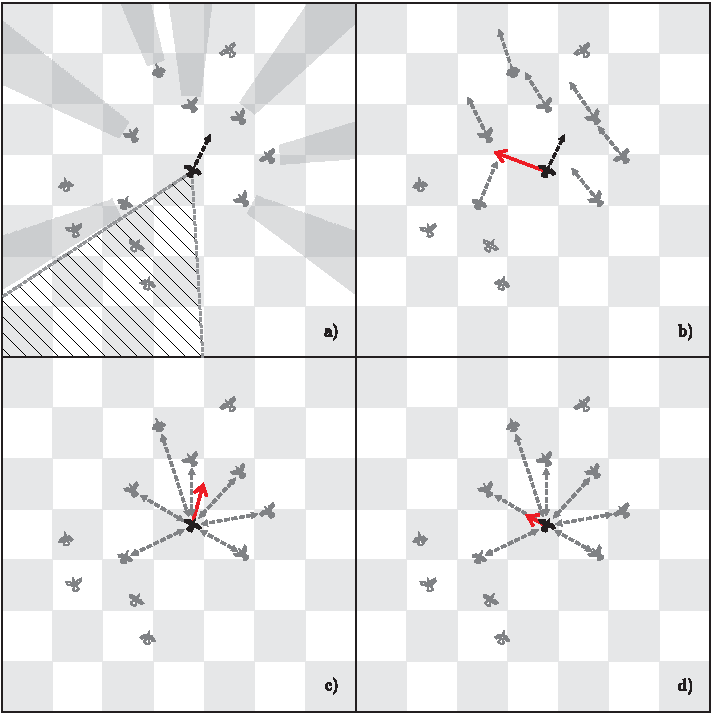
\includegraphics[width=\figurewidth]{alife/basicdrives}
  \caption{Perception of nearby neighbours (a). The black bird is the observed individual. The dark grey birds are the perceived nearby birds that influence the observed bird's behaviour. The white and outlined birds are either occluded by nearer birds (shaded areas), outside of the observed bird's field of vision (dashed area) or outside the number-limited range. Red arrows represent the resulting force vectors of the three basic drives -- lignment (b), cohesion (c), separation (d). The black bird is the observed individual, the dark grey birds are the influencing neighbours.}
  \label{figDrives}
\end{figure}

The original Reynolds' model and most existing models are based on metric distance. In these models every animat within a limited radius influences the behaviour of the observed animat; if an animat is outside that radius it does not have any influence on the observed individual. Nevertheless, recent research \cite{ballerini2008interaction,ballerini2008empirical} suggests that in nature only around seven nearest neighbours influence an individual. As this technique is already gaining support in current state-of-the-art models \cite{hildenbrandt2010selforganized}, we use a number-limited neighbourhood (topological distance) instead of a radius-limited neighbourhood (metric distance) as well. In models based on topological distance, only a fixed number of nearest animats is influential, regardless of their distance.

Our model uses topological distance and concentrates on vision as the principal means of neighbourhood perception. Our animat's field of vision is \ang{300} wide, with a blind angle of \ang{60} directly behind it. Most current models presume that birds have ``perfect'' vision and do not account for the occlusion of distant birds due to other birds flying in the flock. Yet a recent study by Kunz\etal \cite{kunz2012simulations} shows that obstruction of vision increases the realism of simulations. Our model thus takes into account only seven visible (non-occluded) nearby animats (see \figurename~\ref{figDrives}).

Predator and prey behaviours in our study are based on rules extracted from relevant theoretical literature and field observations. We modelled our simulations after a common scenario, where a Peregrine Falcon (\emph{Falco peregrinus}) is attacking a flock of European Starlings (\emph{Sturnus vulgaris}). In horizontal flight, the most economical flight speed (as to the amount of energy spent for flight propulsion) is around 60\% of the bird's maximum speed \cite{tennekes2009simple}. Let us call this speed the \emph{optimal cruising speed}. The optimal cruising speed of European Starling is \mps{11} and the optimal cruising speed of a Peregrine Falcon is \mps{13} \cite{tennekes2009simple}. In accordance to these values we set the maximum speed of our prey animat to \mps{18}, and the maximum speed of our predator animat to \mps{22}. Note that we presumed that the Peregrine Falcon was not hunting by using its characteristic hunting stoop (high speed dive), when it can reach speeds up to \mps{157} \cite{tucker1998gliding}. The minimum flight speed, in nature and in our model, is around 40\% of maximum flight speed \cite{tennekes2009simple}, which results in \mps{7.2} for prey animats and \mps{8.8} for the predator animat. To define the predator-prey relationship we introduced three additional drives -- \emph{hide}, \emph{seek}, and \emph{regulate speed}. The prey's behaviour is governed by the three basic drives (cohesion, separation, and alignment), and in addition hide, and regulate speed (see supplementary material for their explanation). The hide drive helps the prey to survive, as it forces it fly away from the attacking predator; it was tuned so that the direction of the prey's escape matches field observations by Handegard\etal \cite{handegard2012dynamics}. Regulate speed is only active when the hide drive is inactive -- when the predator is hidden from the prey's sight. This drive encourages prey to fly with their optimal cruising speed. The predator's behaviour is guided only by the seek drive (see supplementary material for its detailed explanation). With the seek drive the predator tries to catch the selected target.

\begin{figure}
  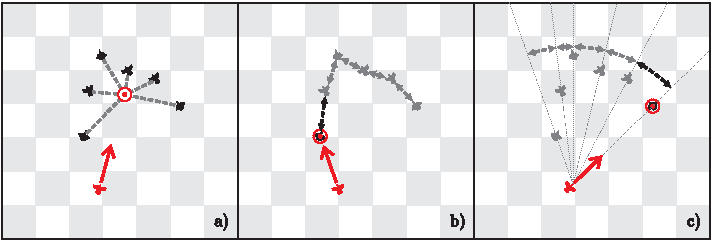
\includegraphics[width=\figurewidth]{alife/strategies}
  \infigurecaption{(a) the predator attacks the centre of the seven perceived prey, (b) the predator attacks the nearest of the seven perceived prey, (c) the predator attacks the most isolated of the seven perceived prey. The red bird is the predator and the red arrow represents the resulting force vector of the predator's seek drive.}
  \caption{The three attack tactics.}
  \label{figStrategies}
\end{figure}

We implemented three different attack tactics (see \figurename~~\ref{figStrategies}). In our first tactic the predator attacks the centre point of the seven perceived prey. This mimics the tactic in which a predator attacks the centre of the flock in hope of hitting a target, but takes into account the limited amount of information available -- distance, relative position, difference in speed, and difference in heading of the perceived artificial animals.

In the second tactic, the predator attacks the nearest of the seven perceived prey. The nearest prey might be the one that is also the fastest to reach therefore making it a logical target for a predator. If a real predator chooses its prey in such a fashion then flocking might work as a mechanism to reduce an individuals' domain of danger \cite{hamilton1971geometry}. The domain of danger is defined as the area in which the observed individual is the predator's nearest neighbour. Obviously the average value of the domain of danger decreases if the number of birds in the flock increases, thus favouring tight highly organized flocks. By reducing the domain of danger an individual lowers the probability of being attacked by the predator, thus possibly increasing its chances of survival.

A predator using the third tactic attacks the most isolated of the seven perceived prey. In our study the most isolated prey is the one that has the largest \emph{angular distance} to its nearest neighbour. We defined angular distance as the angle between a potential target and its nearest neighbour -- from the predator's viewpoint. From a predator's viewpoint, isolated prey appear to have a large domain of danger because they are the most separated from the rest of the perceived prey. From the predator's perspective they would require the largest amount of time to decrease their domain of danger; time that is available to the predator to catch them. If we presume that flocking is indeed a protection mechanism, we can assume that the most isolated bird is the one that is the most vulnerable, making it a logical target for a predator.

%-----
\section{Results and discussion}

To recapitulate, the predator in our model uses one of the following three attack tactics: 1) \emph{attack centre} (\ie attack the centre point of the seven perceived prey), 2) \emph{attack nearest} (\ie attack the nearest of the seven perceived prey), 3) \emph{attack isolated} (\ie attack the most isolated, from the predator's point of view, of the seven perceived prey). In addition to escaping predator attacks and regulating their flight speed the prey can exhibit two types of behaviour: 1) \emph{social} behaviour (\ie prey obey the cohesion, separation, and alignment drives) or 2) \emph{individualistic} behaviour (\ie prey ignore the cohesion and alignment drives, but obey the separation drive to avoid collisions). In total this gives 6 combinations, through which we wished to answer the following questions: 1) what is the optimal predator tactic given a certain prey behaviour, 2) what is the optimal prey behaviour given a certain predator tactic.

\begin{figure}
  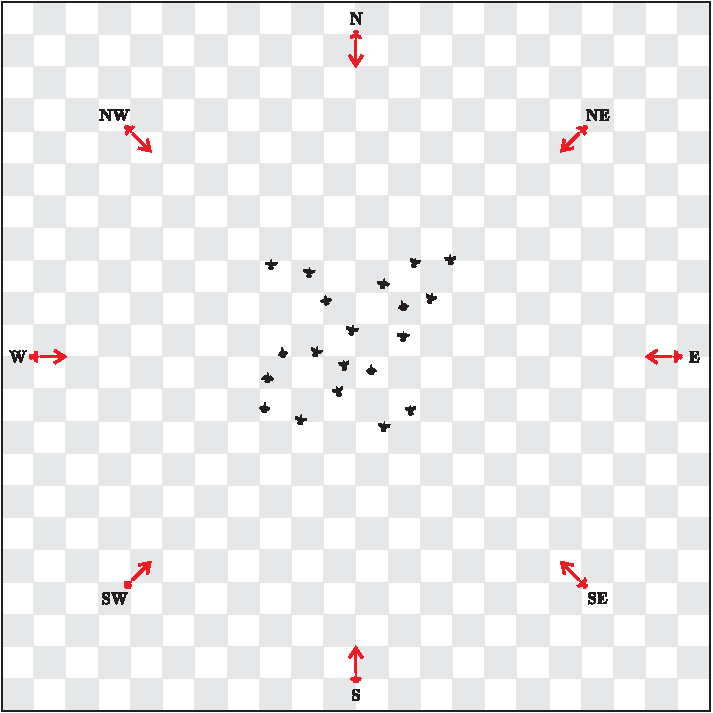
\includegraphics[width=\figurewidth]{alife/bearings}
  \caption{One of the starting configurations along with eight bearings of the predator's attack.}
  \label{figBearings}
\end{figure}

To provide answers to these questions we ran simulations where small cluster flocks consisting of 20, 40 or 60 social or individualistic prey were attacked by a predator from eight different bearings, relative to the flock. One of the starting configurations along with the eight bearings can be seen in \figurename~\ref{figBearings}. The different bearings were used to eliminate any dependency of the simulation's results on the predator's bearing (\eg a head on attack vs an attack from behind). This gives a total of 432 simulations (72 per configuration; selected predator attack tactic and prey behaviour). Each simulation was ran for 900 steps (frames) -- 30 seconds in our visualizations. We measured the time the predator needed to catch a prey. If the predator failed to catch the prey, the time-to-catch was set to 900 frames. The histograms of the time-to-catch for all simulations can be seen in \figurename~\ref{figHistograms}, with a more in depth discussion given in the following subsections.

\begin{figure}
  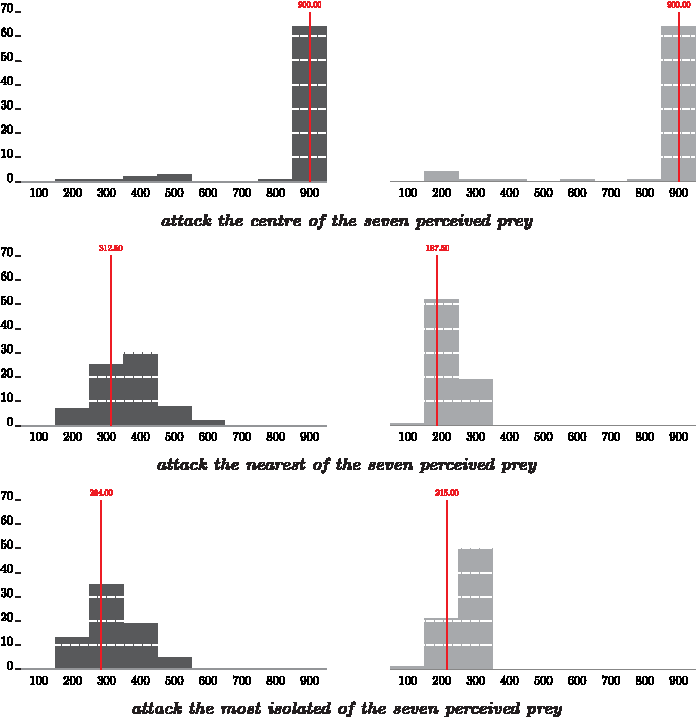
\includegraphics[width=\figurewidth]{alife/histograms}
  \caption{The influence of the predator's attack tactic and prey's behaviour on survivability of prey. Presented are six histograms of the predator's time-to-catch in corresponding simulation runs ($n=72$). Dark grey histograms present the time-to-catch in simulations with social prey, whereas light grey histograms present the time-to-catch in simulations with individualistic prey (cohesion and alignment drives not used). Red lines present the corresponding median time-to-catch.}
  \label{figHistograms}
\end{figure}

%-----
\subsection{Optimal predator tactic}

Our simulations suggest that the best tactic for a predator attacking flocks of social prey is the attack isolated tactic (\ttest{3.01}{142}{0.003}). It would appear that isolated prey benefit the least from the advantages of flocking. On average the predator needed \num{279.74} frames (\SD{72.29}) to catch an isolated prey. The predator whose tactic was to attack the nearest prey, needed \num{316.74} frames (\SD{75.76}) to catch its target, and the one, whose tactic was attack the centre of the seven perceived prey, needed \num{845.08} frames (\SD{165.04}).

With individualistic prey the best tactic for the predator is the attack nearest tactic (\ttest[<]{5.12}{140}{0.0001}). This finding makes sense, since the predator will get to the nearest prey faster than to those that are farther away. Predators that used this, attack nearest, tactic needed, on average, \num{177.31} frames (\SD{33.95}) to catch a prey. Predators that attacked isolated prey caught a prey in \num{208.06} frames (\SD{38.04}). The attack centre tactic proved to be the worst as the predator required \num{832.97} frames (\SD{198.89}) to catch a prey.

The predator that used the attack centre tactic was, in most cases, not successful. In other words it did not catch a prey in the 900 frames for which we ran the simulations (regardless if the prey was social or non-social). Thus the attack centre tactic proved to be the worst tactic regardless of the prey's behaviour.

As for the predator's best tactic overall, regardless of the prey's social or individualistic behaviour, no difference was found between the two most successful tactics, attack nearest and attack isolated (\ttest{0.34}{264}{0.73}).

%-----
\subsection{Optimal prey behaviour}

When the predator used the attack centre tactic no difference was found for the average time-to-catch between social and individualistic prey (\ttest{0.39}{137}{0.69}). In both cases the predator was rarely successful, which is a direct result of the predator's tactic that is based on pure luck.

With predators, whose tactic actually tries to optimize the chance of a positive result, however, the average time-to-catch is higher when prey behaviour is social than when prey behaviour is individualistic, more so when the predator targets the nearest prey (\ttest[<]{14.25}{98}{0.0001}) than when the predator uses the attack isolated tactic (\ttest[<]{7.42}{108}{0.0001}).

The best tactic for prey attacked by a predator appears to be social behaviour.

%-----
\subsection{Biological relevance}

Sonar fine-scale tracking of interactions among predatory fish and their schooling prey performed by Handegard\etal \cite{handegard2012dynamics} suggests that the most successful predators attack from behind. In our simulations, when the predator attacked from the side or front, the prey always managed to escape the initial attack. The predator was successful in one of the successive attacks that occurred from behind. Attacks from behind appear to be much more successful than other strategies as in some cases, when the predator attacked from behind, his initial attack was already fruitful. An example of the corresponding chase and escape paths in the case of a single predator attacking a single prey is presented in \figurename~\ref{figPaths}.

\begin{figure}
  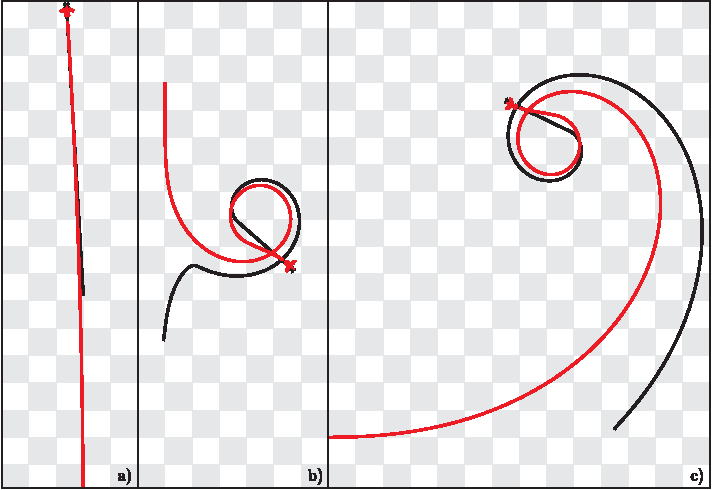
\includegraphics[width=\figurewidth]{alife/paths}
  \caption{Predator attacking a single prey from three main directions: (a) behind, (b) head on, (c) side.}
  \label{figPaths}
\end{figure}

In 1983, Pitcher and Wyche \cite{pitcher1983predator} defined several escape patterns. In our simulations, when the predator attacks the centre point of the seven perceived prey, prey show similar escape patterns as in nature and existing fish school models. Indeed we managed to spot three of the escape patterns defined by Pitcher \& Wyche \cite{pitcher1983predator}: \emph{herd}, \emph{split}, and \emph{fountain}. The herd pattern can be seen at the beginning of a predator approach. The herd pattern then morphs into either split or fountain. Split occurs when a large flock is divided into smaller ones. A typical characteristic of the fountain pattern is that the split flock rejoins behind the predator. These patterns can be seen in \figurename~\ref{figPatternsPhases}.

\begin{figure}
  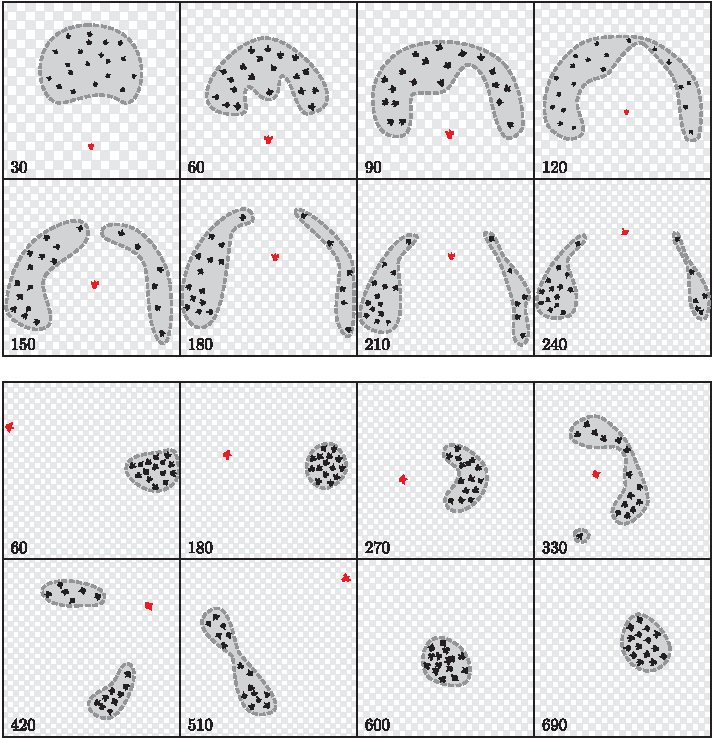
\includegraphics[width=\figurewidth]{alife/patternsPhases}
  \caption{Three common patterns in the artificial flock's response to a predator attack: (above) from \emph{herd} (frames 30--120) to \emph{split} (frames 120--240), (below) from \emph{herd} (frames 60--330) to \emph{fountain} (frames 330--510). In the below snapshots one can also notice the phases in the flock's response: before attack (frame 60), \emph{compression} (frames 60--180 and 510--600), \emph{expansion} (frames 270--510) and \emph{relaxation} (frames 600--690). The red bird is the predator, black birds represent prey. For the sake of clarity the birds were scaled by 200\% (above) and 300\% (below).}
  \label{figPatternsPhases}
\end{figure}

A more quantifiable measure was defined by Lee\etal \cite{lee2006dynamics}, who defined three phases that can be seen in artificial flocks during a predator attack -- \emph{compression}, \emph{expansion} and \emph{relaxation} (\figurename~\ref{figPatternsPhases}). In the first phase of an attack the flock's size decreases; this phase is called compression. In the second phase -- expansion -- prey try to move away from the predator. By doing this, the flock's size increases. In the last phase prey try to regroup, so the flock's size again decreases. This last phase is called relaxation.

The three phases can easily be observed by tracing the artificial flock's \emph{flock size}, as defined by Lee\etal \cite{lee2006dynamics}:
%
\begin{equation}
  \sigma = \sqrt{\frac{\sum_{i=1}^{N}{r_{i}^{2}}}{N}},
\end{equation}
%
where $r_i$ is the distance from the centre of the flock to the $i$-th individual, and $N$ is the total number of animats in the flock. All of our simulations showed a similar response of the artificial flock to a predator's attack. \figurename~\ref{figSizeChart} visualizes how, in our simulations, the flock size changes through time, both when the artificial flock is under threat from the predator and when there is no predator nearby. The flock size is measured in body lengths, one body length equals 20 centimetres, which is the size of a European Starling.

\begin{figure}
  \vskip3pt
  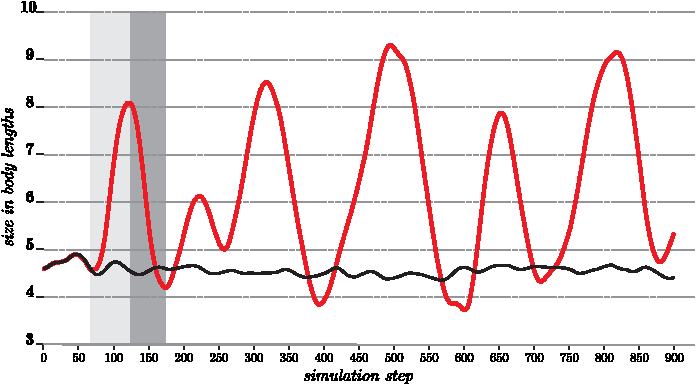
\includegraphics[width=\figurewidth]{alife/sizeChart}
  \infigurecaption{The black line shows the flock size when there is no predator nearby. The red line shows the flock size when the flock is under predator attack.}
  \caption{Plot of the flock size of an artificial flock consisting 20 animats. A clear example of flock expansion is marked with a light grey background, and dark grey is used to mark an example of flock compression. As predator attacks occur one after the other there is no clear example of flock relaxation.}
  \label{figSizeChart}
\end{figure}

%-----
\section{Conclusion}

Our simulations show that the least successful predator is the one that attacks the centre of the flock. They suggest that with predators whose tactic tries to optimize the chance of a positive outcome, social behaviour is more advantageous than individualistic behaviour, which strengthens our belief in the hypothesis that cluster flocking can be a mechanism for protection from predators.

The behaviour of our artificial flocks appears to be comparable with that seen in flocks in nature. The average distance from nearest neighbour is around four body lengths (one body length equals 20 centimetres) \cite{ballerini2008empirical,major1978three,pomeroy1992structure}, the response of an artificial flock to a predator attack is similar to field observations \cite{lee2006dynamics}, and similar escape patterns emerge as in nature \cite{pitcher1983predator}. Our results also shows that the most successful predators attack from behind \cite{handegard2012dynamics}, and seek isolated targets \cite{ioannou2012predatory}.

Our results seem to suggest that cluster flocking around a roost is paradoxical because although its structure might provide some protection against a predator attack, its very existence invites a predator attack, and at least in nature, there are always isolated individuals that can be picked off. It suggests also that at least in some circumstances, which may or may not be common in nature, tight cluster flocking can be of benefit to the flock as a whole, although it does not provide absolute protection to individuals in the flock.

%-----
\chapterAcknowledgements{We sincerely thank Frank H. Heppner of the University of Rhode Island and Maja Lebar Bajec for reading early drafts of the manuscript. Our gratitude also goes to Gregor Šega and Aleksandar Jurišić, who revised the statistical analysis of our results. This work was funded in part by the Slovenian Research Agency (ARRS) through the Pervasive Computing research programme (P2-0395).}

%=====
\begin{subappendices}

%-----
\section{Supplementary material}

In our model the animat is defined as a three stage process \cite{lebarbajec2005fuzzy}: perception, drives, action selection. For each animat the perception stage extrapolates data about the universe (other animats) that is available to the observed animat. In the drives stage, based on these data, a set of actions is computed that would fulfil individual needs of the modelled artificial animal. The action selection stage merges the actions and executes the locomotor response, thus changing the state of the universe.

%-----
\subsection{Perception}

In our model the universe consists of animats only; the universe is in essence a list of animats. To extrapolate data about the universe, as a first step, the observed animat is removed from this list, and the animats remaining in the list sorted based on their distance from the observed animat. Animats hidden by those that are closer to the observed animat or outside its field of view are then filtered out. The nearest seven animats remaining in the list provide the data about the universe. Only information about the relative position (\ie angular offset with respect to the observed animat's heading), distance, speed difference, and heading difference is passed on to the next stage.

Our approach differs from other existing models of number-limited neighbourhood (topological distance) \cite{ballerini2008interaction} in that it always takes into account a fixed number of nearest neighbours. Other models typically implement the number-limited neighbourhood as a \emph{variable} radius-limited neighbourhood \cite{hemelrijk2011somecauses}. In a variable radius-limited neighbourhood the observed animat will increase its radius of perception, if in the previous step it perceived less than the specified number of animats, and decrease it if in the previous step it perceived more than the specified number of animats. This approach in truth varies the number of perceived animats on every step of the simulation, but limits it to the specified number. The principal reason this approach is taken is probably the speed of computation. Its drawback is that the observed animat could potentially perceive all of the other animats, provided these were distributed so that they were all at the same distance from the observed animat.

The number of objects that can be stored in working memory in humans and other mammals is small, 4--7 \cite{ballerini2008interaction,engle1999individual}. The \emph{hippocampus}, the structure in the brain primarily responsible for working memory, is generally similar in birds and mammals \cite{sherry1989hippocampus}. Our use of seven nearest animats in the perceptual world of the prey and predator is thus based on research on working memory. In addition once the predator selects it target, in our model, it filters out all other potential prey, mimicking selective attention \cite{wiederman2012selective}.

%-----
\subsection{Drives}
The drives that result in actions that would fulfil the animat's individual needs are modelled using Mamdani fuzzy rules \cite{mamdani1974application}. For a detailed description of the cohesion, separation, and alignment drives, as well as a brief explanation of how a specific action is computed, the reader is invited to refer to \cite{lebarbajec2005simulating}. An in-depth description is available in \cite{lebarbajec2005fuzzy}.

The data extrapolated in the previous stage are fuzzified as singletons and used as inputs for the fuzzy rules. The fuzzy variables, membership functions, and control rules for the hide drive can be seen in \figurename~\ref{figHide}. \figurename~\ref{figRegulateSpeed} presents the regulate speed drive, and \figurename~\ref{figSeek} presents the seek drive.\footnote{On the membership function charts that describe speed the value $1$ represents the appropriate maximum speed (predator's or prey's) while $-1$ represents the negative value of the appropriate maximum speed. While these are the desired changes in speed, the action selection stage ensures that the current speed of the observed individual never falls under the appropriate minimum speed (predator's or prey's).} The fuzzy rules are evaluated per individual perceived animat and the fuzzy outputs aggregated.

\begin{figure}
  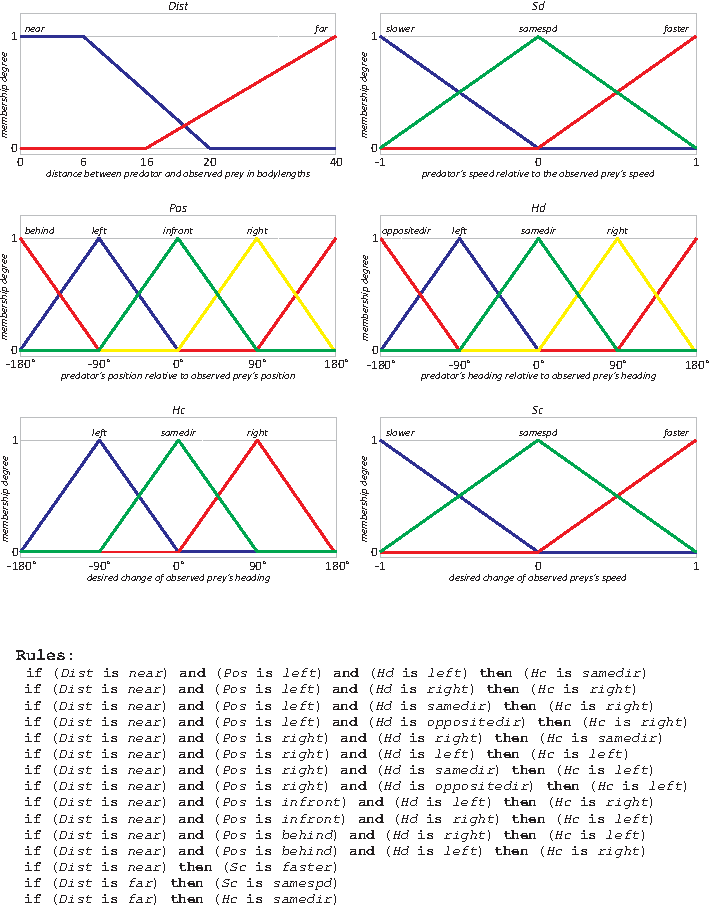
\includegraphics[width=\figurewidth]{alife/hide}
  \caption{Detailed description of the hide drive.}
  \label{figHide}
\end{figure}

\begin{figure}
  \parbox[c][.33\textheight]{\figurewidth}{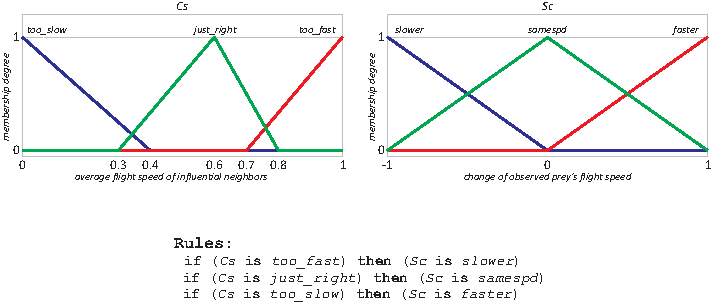
\includegraphics[width=\figurewidth]{alife/regulateSpeed}}
  \caption{Detailed description of the regulate speed drive.}
  \label{figRegulateSpeed}
\end{figure}

\begin{figure}
  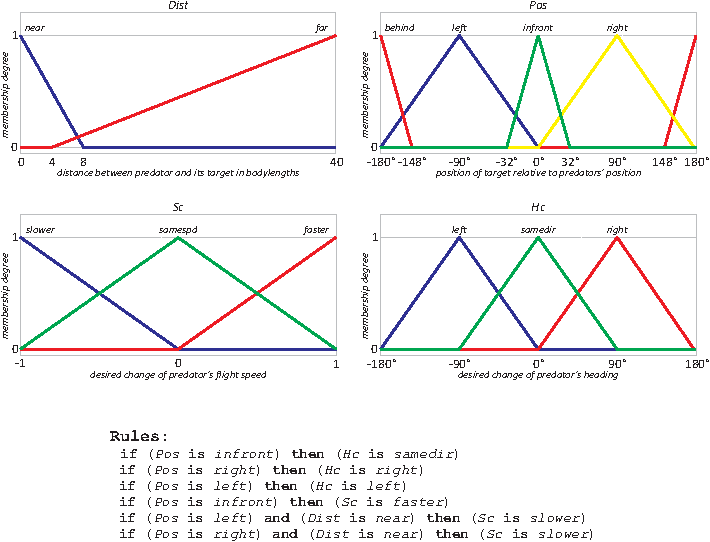
\includegraphics[width=\figurewidth]{alife/seek}
  \caption{Detailed description of the seek drive.}
  \label{figSeek}
\end{figure}

The fuzzy outputs are then defuzzified and a force vector computed. This force vector represents the action that will fulfil the individual need. It gives the direction and magnitude of the individual drive (the desired change in speed and direction).

%-----
\subsection{Action selection}
In the action selection stage the force vectors resulting from individual drives are merged together and a resulting force vector computed. The merging is achieved through a simple weighted sum of the individual force vectors. The resulting force vector is interpreted as a Newtonian force based on which the observed animat's speed, heading and position are updated.

%-----
\subsection{Parameter values}
All of our model's parameters were either extrapolated from relevant theoretical literature (\eg speed, field of view, etc.) or tuned (\eg fuzzy membership functions, action selection mixing weights, etc.) so that the resemblance of the displayed behaviour to that observed in nature was visually as close as possible. For example, the action selection mixing weights have been configured so that the simulations visually resemble (as close as possible) field observations of flocking behaviour. In the prey's case these were (5, 5, 3, 4 and 1) for cohesion, separation, alignment, hide and regulate speed respectively. \tablename~\ref{table:parameters} presents all of the remaining parameters of the model.

\begin{table}
  \caption{Default parameter values.}
  \label{table:parameters}
  \begin{tabular}{l l l}
    \toprule
    Parameter & Description & Default value \\ [0.5ex]
    \midrule
    $\Delta t$ & Time step & 1 frame (\vfrac{1}{30}\,\si{\second}) \\
    $T$ & Maximum length of one simulation & 900 frames (\SI{30}{\second}) \\
    $v_\textnormal{aM}$ & Maximum speed of the predator animat & \mps{22} \\
    $v_\textnormal{am}$ & Minimum speed of the predator animat & \mps{8.8} \\
    $v_\textnormal{pM}$ & Maximum speed of prey animats & \mps{18} \\
    $v_\textnormal{pm}$ & Minimum speed of prey animats & \mps{7.2} \\
    $\varphi$ & Animat field of view & \ang{300} \\
    $n$ & Number of influential nearest neighbours & 7 \\
    $w_\textnormal{c}$ & Weight for cohesion drive & 5 \\
    $w_\textnormal{s}$ & Weight for separation drive & 5 \\
    $w_\textnormal{a}$ & Weight for alignment drive & 3 \\
    $w_\textnormal{e}$ & Weight for hide drive & 4 \\
    $w_\textnormal{rs}$ & Weight for regulate speed drive & 1 \\
    $w_\textnormal{h}$ & Weight for seek drive & 1 \\
    $l$ & Body length & \SI{0.2}{\metre} \\
    \midrule
    & Fuzzification & singleton \\
    & Fuzzy conjunction & product \\
    & Fuzzy disjunction & probabilistic sum \\
    & Fuzzy implication & product \\
    & Fuzzy aggregation & probabilistic sum \\
    & Defuzzification & centrer of gravity \\
    \bottomrule
  \end{tabular}
\end{table}

\end{subappendices}

	% !TeX root = ./thesis.tex










%==============================
\chapter[Simulating predator attacks on schools: evolving composite tactics]{Simulating\\ predator attacks on schools:\\ evolving composite tactics}
\label{chap:ecomod}

\chapterAbstract[published={ecomod/Demšar_etal_2015.pdf}, keywords={Bird, flock, artificial life, boid, fuzzy logic, predator}]{One hypothesis about the origins and evolution of coordinated animal movements is that they may serve as a defensive mechanism against predation. Earlier studies of the possible evolution of coordinated movement in prey concentrated on predators with simple attack tactics. Numerous studies, however, suggest that to overcome the apparent defensive mechanisms which grouping and coordinated movement may provide to prey, predators in nature appear to use elaborate target selection and pursuit/hunting tactics. We here study predators that use composite tactics, a) predators that in successive attacks based on probability choose one of several simple attack tactics, b) predators that first disperse prey and then pick off isolated individuals. We develop an individual based model of a group of prey that is attacked by a solitary predator agent. By using genetic algorithms, we enable the predator agent to adapt a) the probability that a specific tactic will be selected in the next attack, b) the distance at which it stops dispersing the prey and the radius within which it searches for the most isolated prey. With a direct competition of the evolved predator agents we examine which is the better tactic against a group of prey moving in a polarised cohesive manner in three different settings. Our results suggest that, a) a delayed response is an efficient advanced prey defence tactic, b) predator confusion plays an important role in the evolution of composite tactics, and c) when confusion is at play, the dispersing predator is a much better hunter, capable of at least partially diminishing the effectiveness of the prey's delayed response.}

%-----
\section{Introduction}

Collective behaviour is a phenomenon that can easily be observed in nature, where the most typical examples are schools of fish, flocks of birds, swarms of insects, and herds of ungulates. Studies of collective behaviour are interesting not only because they give a better insight into the behaviour of animals, but also because humans behave in a similar fashion in a wide repertoire of situations. Similar behaviour (as in animal groups) can be seen in stop and start traffic jams, crowd behaviour at various events, \eg at football games or music concerts \cite{silverberg2013collective}, and even in the bureaucracy of the European Union \cite{sumpter2006principles}. Comparable patterns can also be observed at much smaller scales like cancerous cells \cite{deisboeck2009collective}.

The literature about collective behaviour contains several hypotheses about why animals coalesce into groups. Some studies suggest that animal groups may increase the mating and foraging efficiency of their members \cite{krebs1994behavioural}, or that grouping could save energy because of hydrodynamic or aerodynamic benefits \cite{bill1976drag,hemelrijk2014increased,lissaman1970formation,partridge1979evidence}. Other studies propose that such groups might function as a defensive mechanism against predators \cite{cresswell2011predicting,larsson2012why,demsar2014simulated,hart2005predator,krause2002living,lebarbajec2009organized,nishimura2000studying,pavlov2000patterns}.

Collective behaviour in animals is in some cases (\eg flocks of birds) quite large in scale and as such hard to enclose in a controlled environment in which scientists could then perform various test of hypotheses about the ``whys'' and ``hows'' of such behaviour of the animal groups \cite{lebarbajec2009organized}. If we look at the case of a solitary predator attacking a group of prey, it is evident that in nature different predators with different hunting tactics exist in different environments, meaning that it is difficult to compare the tactics without the confounding effects of environmental context. As computational approaches usually remove the effects of the environment they proved to be a good tool for studying various hypotheses concerning collective behaviour \cite{couzin2002collective,hildenbrandt2010selforganized,vicsek1995novel}, and the results obtained with such methods are usually more general.

Several computer models suggest that animal grouping may indeed act as a defensive mechanism against predators. Some models \cite{olson2013critical,olson2016evolution,reluga2005simulated,wood2007evolving} focused on the selfish herd theory \cite{hamilton1971geometry} and its effect on the safety of prey individuals. The selfish herd theory suggests that individuals try to reduce their predation risk by reducing their domain of danger, where an individual's domain of danger is defined as the area in which any point is nearer to the observed individual than it is to any other individual \cite{hamilton1971geometry}. A number of studies \cite{kunz2006prey,nishimura2000studying,olson2013predator,zheng2005behavior} suggest that predator confusion might play an important role in defence against predators and evolution of grouping behaviour. Ruxton \& Beauchamp \cite{ruxton2008application} and Haley\etal \cite{haley2014exploring} investigated the many eyes theory, which suggests that as the size of the group increases the amount of time an individual has to scan the environment decreases. As larger groups are usually more conspicuous to the predator, Tosh \cite{tosh2011conditions} concentrated on density dependant selection of individuals in prey aggregations and the dilution of risk theory, which suggests that the chance of a single prey to be targeted is lower in larger groups. Some models \cite{demsar2014simulated,oboshi2003collective,ward2001evolving}, however, did not focus on a specific hypothesis about why animals are safer in groups.

Natural observations \cite{cresswell2011predicting,forsman1998visual,gazda2005division,handegard2012dynamics,hector1986cooperative,nottestad2002digging,kane2014falcons,lopez2006bottlenose,rutz2012predator} suggest that predators can decrease the defensive advantages of grouping by using sophisticated target selection and pursuit/hun\-ting tactics. In turn prey can also use sophisticated escape manoeuvres to increase their chances of survival \cite{domenici2011escapology1,domenici2011escapology2}. For example a fish school often delays its escape response to a later point in time, and then tries to outsmart the predator with rapid movement such as the flash expansion or the fountain effect \cite{partridge1982structure}.

To enhance their chances of a successful hunt goshawks (\emph{Accipiter gentilis}) in large flocks of feral pigeons (\emph{Columba livia}) single out odd-coloured birds as target prey, presumably because targeting rare coloured birds in large uniform flocks might help them overcome confusion \cite{rutz2012predator}. Once a target is selected, some predators in nature also use various pursuit tactics, for example as a recent experimental study reported \cite{kane2014falcons} some species of falcons during pursuit use the technique of motion camouflage. They either camouflage themselves against a fixed background object so that the prey observes no relative motion between them and the fixed object or they approach the prey so that, from the point of view of the prey, they always appear to be on the same bearing \cite{justh2006steering}. While peregrine falcons (\emph{Falco peregrinus}) normally attack from the open and use aerial pursuit, sparrow hawks (\emph{Accipiter nisus}) prefer to ambush prey from cover \cite{cresswell2011predicting}. To increase their hunting success several species have even evolved to hunt their prey by working together with other members of the species \cite{alcock1979animal,handegard2012dynamics,packer1988evolution}. Bottlenose dolphins (\emph{Tursiops truncatus}) have distinctive behavioural roles during group feeding, one individual herds the attacked fish towards the remaining dolphins, to make them leap into the air and become easy prey for the team \cite{gazda2005division,lopez2006bottlenose}. Killer whales (\emph{Orcinus orca}) congregate in large groups, dive to the limit of their capacity, force tens of tons of herrring (\emph{Clupea harengus}) out of their safe deep-water habitat by coordinated action, and split large aggregations of fish into small, dense schools before attacking them \cite{nottestad2002digging}. On the other hand, some predator species that often hunt alone (for example swordfish, \emph{Xiphias gladius}) use a different tactic, and approach the centre of the school to disperse it and when it does, they lock on isolated individuals \cite{larsson2012why,pavlov2000patterns}. Lett\etal \cite{lett2014effects} showed that predators can efficiently disturb fish schools if they attack them with a high enough frequency, however they did not measure how these disturbances influence the predator's hunting success.

Since several empirical studies suggest that predator animals in nature use very elaborate hunting techniques, the simple attack tactics used in previous computer models might be naïve. This research focuses on how a solitary predator might adapt its attack tactic to overcome the defensive benefits provided by collective behaviour and increase its hunting success. To our knowledge, this has been investigated (to some degree) by Nishimura \cite{nishimura2002predator}, Demšar \& Lebar Bajec \cite{demsar2014simulated}, Kunz\etal \cite{kunz2006prey}, and Olson\etal \cite{olson2013critical,olson2013predator,olson2016evolution}, but all of these studies concentrated on simple attack tactics. In this study we use \emph{genetic algorithms} \cite{holland1992adaptation} to investigate the adaptation of a solitary predator that uses composite tactics. First we study the adaptation of a predator that on each individual attack chooses between three simple tactics (attack nearest prey, attack central prey, attack peripheral prey). With this we analyse to which tactic an evolved solitary predator will resort to use the most when released to attack a group of prey moving in a polarised cohesive manner (\emph{mixture of simple tactics}). Next we study the adaptation of a predator that initially chases the nearby group of prey in order to disperse it and then locks on the most peripheral prey the (\emph{dispersing tactic}). More specifically we investigate how the predator adapts the parameters of this composite tactic (\ie the distance at which to stop dispersing and the radius in which to search for the most peripheral target) in order to increase the hunting success. Note that in the case of predators that use the dispersing tactic, the line between target selection and hunting/pursuit tactic becomes less clear, as the predator intentionally defers the decision about its target to a later point in time.

%-----
\section{Methods}

Scientists that use computational approaches to study collective behaviour usually design computer models in which the behaviour of the modelled animals is in most cases constructed around \emph{drives} \cite{lebarbajec2009organized,reynolds1987flocks,vicsek2012collective}. These are designed so that the behaviour of artificial animals in the computer model resembles the behaviour of their counterparts in nature. The drives are implemented in various ways and the parameters of the drives that govern the behaviour of individuals are usually pre-set by hand (\ie \emph{pre-set models}); some researchers, as in our case, however, use genetic algorithms \cite{holland1992adaptation} to let certain parameters evolve through time (\ie \emph{evolvable models}) and by means of that the authors study the possible evolution of collective behaviour or attack tactics.

Since several studies \cite{huth1992simulation,kunz2012simulations} showed that the dimensionality of the model minimally affects the results of the simulations of schooling systems without a predator, our model is for computational simplicity also two-dimensional. It consists of two types of agents -- a solitary predator and a group of prey. The behaviour of an individual depends on its nearby neighbours. The goal of prey individuals is to survive, while the predator tries to catch as many prey individuals as possible. In our model the behaviour of prey is not a part of the evolutionary process, it is pre-set so that the group of prey moves in a polarized cohesive manner; only the behaviour of the predator evolves.

\begin{table}
	\caption{Values for zone radii, weights and other parameters of our model.}
	\label{tab:parameters}
	\begin{tabular}{llll}
		\toprule
		Parameter & Description & Default value & Tested value\\
		\midrule
		Prey\\
		\quad$v_\textnormal{m}$ & Maximum speed of prey & \BLps{4} & \\
		\quad$v_\textnormal{c}$ & Cruising speed of prey & \BLps{2} & \\ 
		\quad$\phi$ & Prey's field of view & \ang{300} & \\
		\quad$r_\textnormal{s}$ & Zone radius for the separation drive & \BL{5} & \\
		\quad$r_\textnormal{a}$ & Zone radius for the alignment drive & \BL{25} & \\
		\quad$r_\textnormal{c}$ & Zone radius for the cohesion drive & \BL{100} & \\
		\quad$r_\textnormal{e}$ & Zone radius for the escape drive & \BL{100} & \BL{50} \\
		\quad$w_\textnormal{s}$ & Weight for the separation drive & \SI{5}{\per\second\squared} & \\
		\quad$w_\textnormal{a}$ & Weight for the alignment drive & \SI{0.3}{\per\second} & \\
		\quad$w_\textnormal{c}$ & Weight for the cohesion drive & \SI{0.01}{\per\second\squared} & \\
		\quad$w_\textnormal{e}$ & Weight for the escape drive & \SI{5}{\per\second\squared} & \SI{12}{\per\second\squared} \\
		\quad$a_\textnormal{m}$ & Prey's maximum acceleration & \BLpss{2} & \\
		\quad$L$ & Body length (\si{\bodylength}) & \SI{0.2}{\metre} & \\
		Predator\\
		\quad$L_\textnormal{p}$ & Predator body length (\si{\predatorbodylength}) & \BL{6} & \\
		\quad$v_\textnormal{mp}$ & Maximum speed of the predator & \BLps{6} & \\
		\quad$v_\textnormal{cp}$ & Cruising speed of the predator & \BLps{3} & \\
		\quad$r_\textnormal{h}$ & Zone radius for the hunt drive & \BL{400} & \\
		\quad$r_\textnormal{co}$ & Confusability radius & \BL{25} & \BL{0}\ \\
		\quad$a_\textnormal{h}$ & Hunting acceleration & \BLpss{2.5} & \\
		\quad$d_\textnormal{c}$ & Catch distance & \PBL{1} (\BL{6}) & \\
		\quad$t_\textnormal{h}$ & Handling time & \SI{30}{\second} & \\
		\quad$t_\textnormal{r}$ & Refocus time & \SI{30}{\second} & \\
		\bottomrule
	\end{tabular}
\end{table}

Our prey and predator models are zone-based \cite{aoki1982simulation,couzin2002collective}, meaning that in the process of calculating the acceleration that represents a particular drive only the individuals that are located within the boundaries of that particular drive's zone are taken into account. The final acceleration that represents the individual's action is a weighted sum of the drives. Parameters of the prey agent were set as in an earlier model \cite{hemelrijk2010emergence} based on empirical research of mullets (\emph{Chelon labrosus}) \cite{videler1993fish}. Following Inada \& Kawachi \cite{inada2002order}, the parameters of the predator agent were set so that it was \num{1.5} times faster than the prey, but we also made it less manoeuvrable \cite{domenici2001scaling}. Preliminary simulations where the predator's speed was equal to that of the prey showed that in this case the predator almost never catches the targeted prey. The only exception is when it approaches an isolated prey directly from behind. In this case the prey is unable to see the predator approaching (as the predator is in its blind spot) and therefore it is not even trying to escape. A short descriptions of all of the model's parameters and their default values can be seen in \tablename~\ref{tab:parameters}.

%-----
\subsection{Prey}

In our model the principal mechanism of neighbourhood perception is vision; the prey's field of view is \ang{300} wide with a blind angle of \ang{60} behind it \cite{fernandezjuricic2004visual,reuter2005selforganization}. The field of view limited neighbourhood is the set of agents that consists of agents that are a) not the observed individual itself, and b) within the \ang{300} degree visual range of the observed individual:
%
\begin{equation}
\set{N} = \{j \in \set{A}|\ j \neq i, \uvec{v}\cdot\uvec{d}_j \geq \vartheta\},
\label{eq:neighbourhood}
\end{equation}
%
where $\set{A}$ is a set consisting of the predator agent and prey agents, $i$ is the observed prey agent, $\vec{v}$ its current velocity and $\uvec{v}=\vec{v}/\|\vec{v}\|$ its current heading, $\uvec{d}_j=(\vec{p}_j-\vec{p})/\|\vec{p}_j-\vec{p}\|$ is the unit direction vector pointing from the current position of the observed prey agent to the current position of agent $j$ and $\vartheta$ is the cosine of the prey's field of view. The field of view limited neighbourhood $\set{N}$ is used for computing the observed individual's drives.

A prey agent has four drives and thus four zones -- \emph{separation}, \emph{alignment}, \emph{cohesion}, and \emph{escape} zone. The separation drive takes into account only prey that are in the separation zone; \ie all prey that are closer than the separation zone radius. The alignment drive takes into account only prey that are in the alignment zone; \ie those that are more distant than the separation zone radius but closer than the alignment zone radius. The cohesion drive takes into account only prey that are in the cohesion zone; \ie those that are more distant than the alignment zone radius but closer than the cohesion zone radius. The escape drive is used in combination with the other drives only if the predator is inside the escape zone; \ie closer than the escape zone radius. In our model the default values for the separation, alignment, cohesion, and escape zone radii are 5, 25, 100 and 100 body lengths (\si{\bodylength}) respectively so prey can perceive other prey and the predator in a radius of \BL{100}.

Each of the four drives returns an acceleration vector that represents the prey's action according to the specific drive. The actual acceleration that is used to update the prey's velocity, is calculated as a weighted sum of all four drives:
%
\begin{equation}
\vec{a}=w_\textnormal{s}\vec{a}_\textnormal{s}+w_\textnormal{a}\vec{a}_\textnormal{a}+w_c\vec{a}_\textnormal{c}+w_e\vec{a}_\textnormal{e},
\end{equation}
%
where $w_\textnormal{s}$, $w_\textnormal{a}$, $w_\textnormal{c}$, $w_\textnormal{e}$ are the weights and $\vec{a}_\textnormal{s}$, $\vec{a}_\textnormal{a}$, $\vec{a}_\textnormal{c}$, $\vec{a}_\textnormal{e}$ the corresponding accelerations for the separation, alignment, cohesion and escape drive respectively. The weights were pre-set to \SI{5}{\per\second\squared}, \SI{0.3}{\per\second}, \SI{0.01}{\per\second\squared} and \SI{5}{\per\second\squared} respectively, so that the prey moved in a cohesive polarised manner. If the length of the acceleration vector exceeds the prey's maximum acceleration (\BLpss{2}) the acceleration vector is shortened so that its length equals the prey's maximum acceleration and the length of the updated velocity vector is kept within the prey's cruising and maximum speed:
%
\begin{eqnarray}
\vec{v}'=[\vec{v}+[\vec{a}]_{[0,a_m]}\Delta t]_{[v_\textnormal{c},v_\textnormal{m}]},\\
\label{eq:v}
\vec{p}'= \vec{p} + \vec{v}'\Delta t,
\end{eqnarray}
%
where $\vec{v}$ is the current velocity of the observed prey agent, $\vec{p}$ its current position, $a_\textnormal{m}$ and $v_\textnormal{m}$ the prey's maximum acceleration and maximum speed, $v_\textnormal{c}$ the prey's cruising speed, $\Delta t$ the simulation time step, $\vec{v}'$ and $\vec{p}'$ the velocity and position of the observed prey agent in the next simulation time step respectively, and
%
\begin{equation}
[\vec{x}]_{[a,b]}=\begin{cases}
a\uvec{x} & \textnormal{iff}\ \|\vec{x}\| < a \\
b\uvec{x} & \textnormal{iff}\ \|\vec{x}\| > b \\
\vec{x} & \textnormal{otherwise,}
\end{cases}
\end{equation}
%
where $\vec{x}$ is a vector and $a$ and $b$ are the lower and upper length bounds.

The three drives, separation, alignment, and cohesion, are the drives that are most commonly used in computer models of collective behaviour \cite{reynolds1987flocks}. The separation drive helps prey avoid collisions. The acceleration that represents the prey's action (change in speed and heading) according to this drive is defined as:
%
\begin{equation}
\vec{a}_\textnormal{s}=\frac{1}{|\set{N}_\textnormal{s}|} \sum_{j \in \set{N}_\textnormal{s}}\left(-\uvec{d}_j\left(1-\frac{\|\vec{d}_j\|}{r_\textnormal{s}}\right)\right),\quad 
\set{N}_\textnormal{s} = \{j \in \set{N}|\ j \neq p,\ \|\vec{d}_j\| \leq r_\textnormal{s} \},
\end{equation}
%
where $j$ is an influencing neighbour, $p$ the predator, $\vec{d}_j=\vec{p}_j-\vec{p}$ is the offset vector pointing from the current position of the observed prey agent to the current position of agent $j$, $r_\textnormal{s}$ is the separation zone radius and $\set{N}$ the field of view limited neighbourhood as defined in \eq~\eqref{eq:neighbourhood}.

With the alignment drive, prey synchronize their velocities. The acceleration that represents the prey's action is defined as:
%
\begin{equation}
\vec{a}_\textnormal{a}=\left(\frac{1}{|\set{N}_\textnormal{a}|} \sum_{j \in \set{N}_\textnormal{a}} \vec{v}_j\right)-\vec{v},\quad 
\set{N}_\textnormal{a}=\{j \in \set{N}|\ j \neq p,\ r_\textnormal{s} \leq \|\vec{d}_j\| \leq r_\textnormal{a} \},
\end{equation}
%
where $\vec{v}$ is the velocity of the observed prey agent, $\vec{v}_j$ is the velocity of agent $j$ and $r_\textnormal{a}$ is the alignment zone radius.

The cohesion drive simulates attraction toward distant prey and the acceleration that represents the prey's action is defined as:
%
\begin{equation}
\vec{a}_\textnormal{c}=\frac{1}{|\set{N}_\textnormal{c}|} \sum_{j \in \set{N}_\textnormal{c}} \vec{d}_j,\quad \set{N}_\textnormal{c}=\{j \in \set{N}|\ j \neq p,\ r_\textnormal{a} \leq \|\vec{d}_j\| \leq r_\textnormal{c} \},
\end{equation}
%
where $r_\textnormal{s}$ is the separation zone radius.

The escape drive represents the prey's tendency to escape from the predator. It is represented as the acceleration away from the predator's current position, and calculated as
%
\begin{equation}
\vec{a}_\textnormal{e}=\begin{cases}
-\uvec{d}_p\left(1-\frac{\|\vec{d}_p\|}{r_\textnormal{e}}\right) & \textnormal{iff}\ p \in \set{N} \wedge \|\vec{d}_p\| \leq r_\textnormal{e}\\
\vec{0} & \textnormal{otherwise,}
\end{cases}
\end{equation}
%
where $p$ is the predator and $r_\textnormal{e}$ is the escape zone radius.

The maximum speed of prey was set to \BLps{4}, and the cruising speed was set to \BLps{2}, the cruising speed of mullets \cite{videler1993fish}. Zone sizes and zone weights were set in a way that when prey was not under the threat of predation, prey moved in a synchronized cohesive manner while maintaining an inter-individual distance of 1--2 body lengths \cite{johansen2010kinematics,killen2011aerobic}.

%-----
\subsection{The predator}
 
During foraging in nature some avian visual sit-and-wait predators \cite{gall2010visual,orourke2010hawkeyes2} scan the neighbourhood by turning their head, while some aquatic predators reduce travel speed and increase turning rate in areas where resources are relatively more abundant, a behaviour termed ``area-restricted search'' \cite{thums2011insitu}. Some avian visual predatory species in nature have a higher visual acuity than prey and detect prey at far distances \cite{andersson2009predator}, while some aquatic predators, \eg swordfish (\emph{Xiphias gladius}), warm their retina to significantly improve temporal resolution, and hence the detection of rapid motion \cite{fritsches2005warm}. Since the goal of this research is not the investigation of the relationship between the predator foraging strategy and prey encounter/foraging success, but rather the target selection tactics and hunting success the predator field of view in our model is \ang{360} wide -- there is no blind angle. Additionally, in order to diminish the occurrences when the predator ``did not see a potential prey'' our predator agent can perceive prey in a radius of \BL{400}.

Like in other studies \cite{demsar2014simulated,kunz2006prey,nishimura2002predator,olson2013predator} our study focuses on the target selection phase of the predator attack. Once the target is selected, the predator uses classical pursuit \cite{nahin2012chases} to chase the prey, \ie it heads directly toward the evading prey, so that the image of the prey is centred on its visual field. Thus the behaviour of the predator is governed only by the hunt drive; the \emph{hunt} drive is defined as an acceleration that points towards the position of the current target:
%
\begin{equation}
\vec{a}_h=\begin{cases}
a_\textnormal{h} \uvec{d}_t & \textnormal{iff}\ \|\vec{d}_t\| \leq r_\textnormal{h} \\
\vec{0} & \textnormal{otherwise,}
\end{cases}
\end{equation}
%
where $t$ is the target prey agent, $a_\textnormal{h}$ is the hunting acceleration, and $r_\textnormal{h}$ the hunt zone radius. Which prey is targeted depends on the predator's tactic -- see sections \ref{sec:mix} (\nameref{sec:mix}) and \ref{sec:dispersing} (\nameref{sec:dispersing}). 

The predator moving forward at its current velocity with no change in heading when it does not see any prey, might appear an unrealistic foraging pattern for predators. However, as our study did not concentrate on foraging patterns when there is no potential prey nearby but rather on target selection and hunting tactics when multiple potential prey are visible, the handling time, refocus time and perception radius of the predator were set to be such that the occasions when the predator ``did not see a potential prey'' were extremely rare.

Since the predator uses only the hunt drive, \eq~\eqref{eq:v} in the case of the predator becomes
%
\begin{equation}
\vec{v}'=[\vec{v}+\vec{a}_\textnormal{h}\Delta t]_{[v_\textnormal{cp},v_\textnormal{mp}]},
\end{equation}
%
where $\vec{v}$ is the current velocity of the predator agent, $v_\textnormal{cp}$ and $v_\textnormal{mp}$ are the predator's cruising and maximum speed respectively, and $\vec{v}'$ is the predator's velocity in the next simulation time step. Other than that the process of updating the velocity and position of the predator agent is the same as in the case of the prey agent.

The maximum speed of the predator agent was set to \BLps{6}, and its cruising speed to \BLps{3}. So just like in Inada \& Kawachi's \cite{inada2002order} model of fish schooling, the predator agent was \num{1.5} times faster than prey agents. Since in nature predators are usually faster, but less manoeuvrable \cite{domenici2001scaling} we set the hunting acceleration to \BLpss{2.5} so that the same holds for our model.

%-----
\subsection{Experiments}

Our experiments can be described as a two-phase cycle composed of 1) the evaluation phase, and 2) the evolution phase. The experiments were run with a population of 100 solitary predators. During the evaluation phase each of these 100 predators (current generation) was released to solitarily attack five different groups of prey. On each occasion it was observed for 600 time steps. The performance of a predator was recorded by counting the cumulative number of caught prey from the five attacked groups. Once the current generation of predators completed their runs, the evaluation phase finished and the evolution phase began. In the evolution phase a new generation consisting of the same number of predators was generated from the current generation of predators. For each predator in the new generation two predators from the current generation were chosen as its parents. Predators that had a higher fitness, \ie caught more prey during the evaluation phase, had a higher chance to be selected as parents. The two parent predators were merged using the cross-over operator, a technique that mixes tactic specific parameters of both parents to create an offspring \cite{holland1992adaptation}; a new predator. Occasionally the tactic specific parameters of the offspring mutated (their values changed slightly). The two-phase cycle was then repeated with the new generation of predators.

Each experiment lasted 500 such cycles (500 generations) and was repeated 20 times. Default values for the mutation rate, mutation factor and other genetic algorithm parameters are given in \tablename~\ref{tab:parameters:ga}. Our preliminary simulations using various mutation rates ranging from 1\% to 5\% matched with the general knowledge about genetic algorithms. In general the final result was very similar for all of the tested mutation rates. A lower mutation rate resulted in less noise in the evolved parameters but the algorithm needed more time (more generations) to produce the near optimal solution. Since in our case we are more interested in the general resulting behaviour rather than the exact parameter values we can afford some noise in the parameter values. The preliminary tests revealed that the mutation rate of 2\% gives good results while keeping the time complexity of the algorithm in reasonable limits.

\begin{table}
	\caption{Values for the parameters used in our experiments.}
	\label{tab:parameters:ga}
	\begin{tabular}{lp{.55\textwidth}l}
		\toprule
		Parameter & Description & Default value \\
		\midrule
		$\Delta t$  & Time step & \SI{1}{\second} \\
		$T$ & Duration of the evaluation phase per predator & 600 time steps \\
		$N_\textnormal{a}$ & Number of groups attacked by predators of one generation & 5 \\
		$N_\textnormal{g}$ & Number of generations & 500 \\
		$m_\textnormal{r}$ & Mutation rate & 2\% \\
		$m_\textnormal{f}$ & Mutation factor (``intensity of mutations'') & 20\% \\
		$n_\textnormal{a}$ & Number of prey individuals in the group & 100 \\
		$n_\textnormal{p}$ & Predator population size & 100 \\
		$D$ & Initial predator's distance from the centre of the prey group & \BL{200} \\
		$S$ & Initial area of the prey group & \SI{100}{\bodylength\squared} \\
		\bottomrule
	\end{tabular}
\end{table}

The five groups of prey, that a predator was released to attack in the evaluation phase, were the same for the whole population of predators in one repetition of the evaluation phase, but were different for each repetition of the two-phase cycle. Each of the five groups consisted of 100 prey randomly distributed within a square area of \SI{100}{\bodylength\squared} (\figurename~\ref{fig:setup}). The velocity vector, which determines the heading and speed of prey, was generated so that the headings of prey had already been approximately aligned before the first attack of the predator. To achieve this, the preys' speeds were set to a uniformly distributed random number between the prey cruising and maximum speed (2 and \BLps{4}) and the preys' headings were set to north rotated by a uniformly distributed random number between \SI{\pm0.05}{\radian}. The predator's first attack was from behind \cite{demsar2014simulated,handegard2012dynamics} (\ie from the south), its starting position was located \BL{200} south from the centre of the prey group and its heading was north towards the centre of the group. The predator's speed was set to a uniformly distributed random number between its cruising and maximum speed (3 and \BLps{6}).

\begin{figure}
	\includegraphics[width=.5\textwidth]{ecomod/fig1}
	\caption{An example of a starting configuration, where the black triangle represents the predator; its bearing is north. The shaded area is the area in which the prey group is generated. Grey dots are the prey, and the grey arrow is their average bearing.}
	\label{fig:setup}
\end{figure}

When the predator selected a target it started hunting it. Which target was selected depended on the predator's tactic -- see sections \ref{sec:mix} (\nameref{sec:mix}) and \ref{sec:dispersing} (\nameref{sec:dispersing}). The predator kept hunting the same target until the target was caught, the predator got confused, the target escaped from the predator's hunting zone radius, or the simulation time (600 steps) ran out. When the predator came close to the target, \ie within a distance that was less than the catch distance it made an attempt to catch the prey. The probability that this attempt was successful was inversely proportional to the number of individuals within the predator's confusability zone \cite{olson2013critical,olson2013predator}:
%
\begin{equation}
P_\textnormal{success}=\frac{1}{|\set{N}_\textnormal{co}|},\quad \set{N}_\textnormal{co}=\{j \in \set{A}|\ j \neq p,\ \|\vec{d}_j\| \leq r_\textnormal{co} \},
\label{eq:confusability}
\end{equation}
%
where \set{A} is the set consisting of the predator agent and prey agents, $j$ is a prey agent, $\vec{d}_j=\vec{p}_j-\vec{p}$ is the offset vector pointing from the current position of the observed agent (the predator) to the current position of agent $j$, and $r_\textnormal{co}$ is the predator's confusability zone radius.

In order to take into account the effort required to eat the prey, the predator did not look for a new target prey immediately after it had successfully caught one. A certain amount of simulation time steps, \emph{handling time} (see \tablename~\ref{tab:parameters}), had to pass before the predator selected a new target. If the predator failed to catch the targeted prey due to confusion a certain amount of simulation time steps, \emph{refocus time} (see \tablename~\ref{tab:parameters}) had to pass as well. If, however, the currently targeted prey would escape from the predator's field of view, the predator would immediately select a new target. Note that due to the choice of the model parameters, more specifically the predator and prey maximum speeds, in our model this does not happen.

In nature there are many types of prey behaving in many different ways and presumably if predators use sophisticated target selection and pursuit/hunting tactics, the prey might use sophisticated escape manoeuvres to outsmart the predator. Indeed a number of studies \cite{kunz2006prey,nishimura2002predator,olson2013predator,zheng2005behavior} suggest that confusion might play an important role in the evolution of grouping behaviour. For these reasons we ran three sets of evolutions of the two composite tactics, a) with parameters set to their default values as listed in \tablename~\ref{tab:parameters}, b) with the prey escape zone set to \BL{50}, the weight of the escape drive set to \SI{12}{\per\second\squared} and the rest of the parameters set to default, and c) with $P_\textnormal{success}$, \eq~\eqref{eq:confusability}, set to be always equal to 1 and the rest set to default. The first case, named \emph{default prey}, represents the typical scenario of a solitary predator attacking a group of prey. The second case, named \emph{prey with delayed response}, represents a group of prey that allows the solitary predator to get close and then performs a rapid escape manoeuvre. The third case, named \emph{non-confusing prey}, investigates if confusability might play a role in the evolution of target selection and pursuit/hunting tactics as well.

%-----
\subsection{Mixture of simple tactics}
\label{sec:mix}

In the first part of our research, the predator that used a mixture of simple tactics was based on similar tactics as predators presented in previous research \cite{demsar2014simulated,nishimura2002predator}: attack nearest prey, attack the most peripheral prey, and attack the most central prey. The nearest prey was simply the one that was the closest to the predator. To determine which prey was most peripheral or central we used the measure of peripherality. In previous research \cite{hemelrijk2000towards,hemelrijk2005individual,hildenbrandt2010selforganized} this measure was called centrality, but since a lower degree of centrality means that the individual is more central and less peripheral, the term peripherality is more appropriate. Peripherality of prey agent $i$ is calculated as the length of $\vec{P}_i$, \ie the average vector of direction towards the group of potentially influencing neighbours:
%
\begin{equation}
\vec{P}_i=\frac{1}{|\set{G}|} \sum_{j \in \set{G}} \uvec{d}_j,\quad \set{G}=\{j \in \set{A}|\ j \neq i,\ j \neq p,\ \|\vec{d}_j\| \leq r_\textnormal{c}\},
\label{eq:peripherality}
\end{equation}
%
where $i$ is the observed prey agent, $j$ is an agent, $p$ is the predator agent, $\uvec{d}_j=\vec{d}_j/\|\vec{d}_j\|$ the unit vector pointing from the current position of the observed agent (prey agent $i$) to the current position of agent $j$, $r_\textnormal{c}$ the prey's cohesion zone radius and $\set{G}$ the set of potentially influencing neighbours of the observed prey agent. If a prey agent was isolated (\ie the set of potentially influencing neighbours was empty) its peripherality was set to $+\infty$, meaning that the predator that targeted peripheral targets preferred to attack isolated targets \cite{ioannou2012predatory,demsar2014simulated}.

The prey that is the nearest is simply the one whose distance from the predator is the smallest: 
%
\begin{equation}
t_\textnormal{n}=t:\ \|\vec{d}_t\|=\min_{j \in \set{T}}\|\vec{d}_j\|,\ \set{T}=\{j \in \set{A}|\ j \neq p,\ \|\vec{d}_j\| \leq r_\textnormal{h}\}.
\end{equation}

The prey that is the most central is the one with the lowest measure of peripherality:
%
\begin{equation}
t_\textnormal{m}=t:\ \|\vec{P}_t\|=\min_{j \in \set{T}}\|\vec{P}_j\|,\ \set{T}=\{j \in \set{A}|\ j \neq p,\ \|\vec{d}_j\| \leq r_\textnormal{h}\}.
\end{equation}

By definition the prey that is the most peripheral is the one with the highest measure of peripherality. However, as the measure of peripherality is defined via the prey's cohesion zone radius (\ie the set of potentially influencing neighbours) and does not consider the predator's angle of approach an additional constraint was taken into account. Only prey whose peripherality vector was pointing in the same direction (\ang{\pm90}) as the unit vector pointing from the current position of the predator to the current position of the prey agent were regarded as possible targets:
%
\begin{equation}
t_\textnormal{p}=t:\ \|\vec{P}_t\|=\max_{j \in \set{T}}\|\vec{P}_j\|,\ \set{T}=\{j \in \set{A}|\ j \neq p,\ \|\vec{d}_j\| \leq r_\textnormal{h},\ \uvec{d}_j\cdot\uvec{P}_j>0\}.
\end{equation}

With this constraint we prevented the predator agent from targeting prey that were on the opposite side of the group (as viewed from the predator's point of view), because in nature they would probably not be visible to the predator.

\begin{table}
	\caption{Parameters that evolve during the evolution of a simple predator.}
	\label{tab:mix}
	\begin{tabular}{llll}
		\toprule
		Parameter & Description & Interval & Initial value \\
		\midrule
		$p_\textnormal{n}$ & Target the nearest prey probability & $[0, 1]$ & Random \\
		$p_\textnormal{m}$ & Target the most central prey probability & $[0, 1]$ & Random \\
		$p_\textnormal{p}$ & Target the most peripheral probability & $[0, 1]$ & Random \\
		\bottomrule
	\end{tabular}
\end{table}

The chromosome of the predator, which was used to construct a generation of predators, consisted of probabilities that determined the likelihood that the predator will use a particular tactic (\ie the probabilities represent genes in the chromosome). Every predator had three probabilities -- one for each of the three tactics, see \tablename~\ref{tab:mix}. For the initial generation of predators the probabilities were assigned normalized uniformly distributed random values between 0 and 1 (see \tablename~\ref{tab:mix}) so that the sum of all probabilities was equal to 1:
%
\begin{equation}
p_\textnormal{n}=\frac{\xi_\textnormal{n}}{\xi_\textnormal{n}+\xi_\textnormal{p}+\xi_\textnormal{m}},\quad p_\textnormal{m}=\frac{\xi_\textnormal{m}}{\xi_\textnormal{n}+\xi_\textnormal{p}+\xi_\textnormal{m}},\quad p_\textnormal{p}=\frac{\xi_\textnormal{p}}{\xi_\textnormal{n}+\xi_\textnormal{p}+\xi_\textnormal{m}},
\end{equation}
%
where $\xi_\textnormal{n}$, $\xi_\textnormal{m}$, $\xi_\textnormal{p}$ are uniformly distributed random values between 0 and 1, and $p_\textnormal{n}$, $p_\textnormal{m}$, $p_\textnormal{p}$ are the probabilities that the predator will attack the nearest, the most peripheral, and the most central target respectively. As already stated, at the start of an evaluation phase, the predators had no target. In the initial step of the evaluation phase the predator selected a target as:
%
\begin{equation}
t=\begin{cases}
t_\textnormal{n} & \textnormal{iff}\  \xi \in (0,p_\textnormal{n}]\\
t_\textnormal{m} & \textnormal{iff}\  \xi \in (p_\textnormal{n},p_\textnormal{n}+p_\textnormal{m}]\\
t_\textnormal{p} & \textnormal{iff}\  \xi \in (p_\textnormal{n}+p_\textnormal{m},1],
\end{cases}
\label{eq:target}
\end{equation}
%
where $\xi$ is a uniformly distributed random value in the interval $(0, 1]$, $t_\textnormal{n}$, $t_\textnormal{m}$, $t_\textnormal{p}$ are the nearest, the most central, and the most peripheral prey respectively. The target selection process, \eq~\eqref{eq:target}, was repeated every time a) the predator's attempt to catch the targeted prey was unsuccessful and the refocus time passed, or b) the predator caught the targeted prey and the handling time passed. That means that the predator could use different simple tactics on successive attacks during one simulation run (600 time steps).

In the evolution phase the chromosome of a new predator (offspring) was generated by using the coin-flip crossover, a type of crossover operator that chooses a gene from one of the parents at random (uniform distribution). The coin-flip crossover was repeated for all genes. Occasionally, being governed by the mutation rate (2\% per parameter), the genes mutated. The mutation of a specific gene, \ie probability of a specific tactic, was simulated as either an increase or a decrease (chosen at random) of the likelihood that the predator will use that particular tactic. The amount of increase/decrease was governed by the mutation factor (20\%). Because the cross-over and mutation could lead to the sum of probabilities not being equal to 1, the last step in the creation of a new chromosome was renormalization, \ie division of individual probabilities by their sum.

%-----
\subsection{The dispersing tactic}
\label{sec:dispersing}

In the second part of our study the predator's tactic was as follows. Initially (\figurename~\ref{fig:dispersing}) the predator chased the centre of the nearby group. The nearest prey (with respect to the predator) and all prey within this prey's set of potentially influencing neighbours, $\set{G}$ in \eq~\eqref{eq:peripherality}, were interpreted as the nearby group. The prey within this group that had the lowest measure of peripherality, \eq~\eqref{eq:peripherality}, \ie was the most central, was interpreted as the group's centre. The nearby group and its centre were determined once per attack and remained unchanged for the duration of the attack. Once the distance of the nearby group's centre was less than the \emph{lock-on distance} the predator locked on the most peripheral prey within its \emph{lock-on radius} (\tablename~\ref{tab:dispersing}). The locked-on individual was then hunted until captured, or the attempt failed due to confusion.

\begin{table}
	\caption{Parameters that evolve during the evolution of the dispersing predator.}
	\label{tab:dispersing}
	\begin{tabular}{llll}
		\toprule
		Parameter & Description & Interval (\si{\bodylength}) & Initial value\\
		\midrule
		$d_\textnormal{l}$ & Lock-on distance & $[0, 400]$ & Random\\
		$r_\textnormal{l}$ & Lock-on radius & $[0, 400]$ & Random\\
		\bottomrule
	\end{tabular}
\end{table}

\begin{figure}
	\vskip.4in % add top and bottom whitespace so that the caption does not overflow the figure box 
	\includegraphics[width=.95\figurewidth]{ecomod/fig2}
	\vskip.4in
	\caption{The dispersing tactic; a predator (black triangle) that uses this tactic initially (a) chases the most central prey (light grey dot) in the nearby group of prey, grey dots, (\ie prey that are within the cohesion zone radius, shaded area, of the nearest prey, black dot). When the predator comes close enough (b), \ie within lock-on distance, dotted circle, it selects as its target prey the most peripheral prey within its lock-on zone radius, shaded area.}
	\label{fig:dispersing}
\end{figure}

During the evolution phase the predators that caught more prey in the evaluation phase had a higher chance of being selected as parents. The offspring predator inherited the value of the lock-on distance from the first parent and the value of the lock-on radius from the second parent. Once in a while the parameters would mutate; the probability of mutation was governed by the mutation rate (2\% per parameter). The mutation was in the form of either an increase or decrease (chosen at random) and the amount was governed by the mutation factor (20\%). The parameters that evolved during our experiments and their initial values can be seen in Table \ref{tab:dispersing}.

%-----
\section{Results and Discussion}

\paragraph{Mixture of simple tactics} In the first part of our research we investigated which of the simple tactics an evolved solitary predator will resort to use the most. This was measured by observing the probabilities that determined the likelihood that a particular tactic would be employed. \figurename~\ref{fig:mix:evo} shows the averages and bootstrapped 95\% confidence interval of the 20 runs for the cases of default prey, prey with delayed response and non-confusing prey. 

\begin{figure}
	\includegraphics[width=\figurewidth]{ecomod/fig3}
	\infigurecaption{Averages and the bootstrapped 95\% confidence intervals based on 20 replicates of our experiments in three different settings -- predators facing a group of prey with default parameters as in Table \ref{tab:parameters} (default prey), predators facing a group of prey with a delayed response, and predators with confusability radius set to 0 (non-confusing prey).}
	\caption{Evolution of the probabilities that determine the likelihood that the predator will use a particular simple tactic when choosing its next target.}
	\label{fig:mix:evo}
\end{figure}

As it can be seen, in the case of default prey, an evolved predator (predator of the last, 500th, generation) attacked almost exclusively the most peripheral prey, 96\% \ci{95.6}{96.9}, meaning that during the course of the evolution predators that attacked the most peripheral targets were more successful than those whose ratio of attacking the nearest or most central prey was higher. For this reason the probability of using these two tactics was very low, 2\% \ci{1.9}{3} and \num{1.3}\% \ci{1}{1.7}, respectively.

In the case of prey with delayed response the evolved predator again mainly attacked the most peripheral prey, 84\% \ci{75}{88.5}. The decrease in probability was mostly due to the increase of the probability of attacking the nearest prey, 12\% \ci{7.3}{20.8}, while the probability of attacking the most central prey still remained very low 4\% \ci{3.6}{4.8}. The adaptation seems quite reasonable as due to the prey's delayed response there is also a higher chance of success when attacking the nearest prey as it might not be able to escape due to overcrowding.

In the case of non-confusing prey, however, the evolved predator adapted to attacking the most central, 55\% \ci{37.5}{71.3}, and nearest prey, 40\% \ci{23.4}{56}. In this case the probability of attacking the most peripheral prey was very low 5\% \ci{4.3}{6}. This result again seems reasonable as attacking peripheral prey builds on the reduction of the chance of the predator getting confused due to the abundance of prey in the vicinity of the chosen target.

\paragraph{Dispersing tactic} In the second part of our research we investigated how an evol\-ving solitary predator that uses the dispersing tactic will adapt the distance at which it will stop chasing the centre of the nearest group and select its actual target prey individual, as well as the radius within which it will search for it. In \figurename~\ref{fig:dispersing:evo}, which shows the means and bootstrapped 95\% confidence interval of the 20 runs for the cases of default prey, prey with delayed response and non-confusing prey, it can be seen that in the case of default prey the evolved predator (predator of the last, 500th, generation) stopped chasing the centre of the nearest group when \BL{19} \ci{18.5}{20.2} from it. Then it locked-on the most peripheral prey in a radius of \BL{129} \ci{112.4}{147}.

\begin{figure}
	\includegraphics[width=\figurewidth]{ecomod/fig4}
	\infigurecaption{Averages and the bootstrapped 95\% confidence intervals based on 20 replicates of our experiments in three different settings -- predators facing a group of prey with default parameters as in Table \ref{tab:parameters} (default prey), predators facing a group of prey with a delayed response, and predators with confusability radius set to 0 (non-confusing prey).}
	\caption{Evolution of the lock-on distance and lock-on radius in the case of the dispersing predator.}
	\label{fig:dispersing:evo}
\end{figure}

In the case of prey with delayed response the chasing stopped when \BL{12.8} \ci{11}{14.4} away from the centre of the nearest group and the final target was searched within \BL{103} \ci{77.8}{129.4}. Interestingly, in the case of prey with delayed response, the predator adapted to dive significantly deeper \BLpss{2.5} (\ttest{-6.7227}{29.757}{9.832e-8}) but there was no significant difference between the radii within which the final targets were chosen (\ttest{-1.6589}{33.869}{0.1064}).

In both cases the predator locked on its target when it came quite close to the centre of the nearest group. As possible values for the lock-on distance ranged from 0 to \BL{400} we can assume that dispersing a school, flock or herd greatly reduces its defensive benefits. When the evolved predator locked on its target, it locked on the most peripheral prey in a radius that is lower than the midpoint of possible values (0 to \BL{400}), therefore we can assume that in both cases the dispersing predator preferred isolated but somewhat nearby prey. This suggests that the best potential targets might be prey that are close to the periphery of a school, flock, or herd while at the same time somewhat close to the predator.

In the case of non-confusing prey, however, the chasing stopped when \BL{153} \ci{148.5}{156.3} from the centre of the nearest group, and the final target was searched within \BL{151} \ci{147.6}{154}. Surprisingly there was no significant difference between the two parameters (\ttest{0.561}{36.83}{0.5782}). What is even more interesting is that the values are close to the midpoint of possible values (0 to \BL{400}), and since there is no significant difference between the two values, the end result is a behaviour very similar to attacking the nearest prey. Note that the dispersing predator initially chases the centre of the nearest group and when close enough locks-on the most peripheral target within the lock-on radius. Since the lock-on radius and lock-on distance are very similar, the end result is that the nearest prey and most peripheral prey within the searched radius often coincide.

\paragraph{Comparison between tactics via direct competition} In the third part of our research we used direct competition in order to assess the quality of the evolved tactics from the predator's point of view. Each individual predator that emerged from the 20 replicates of an experiment (mixture of simple tactics, and dispersing tactic) was released to independently attack the same \num{1000} distinct groups of prey, each for 600 time steps and the number of caught prey recorded. This was repeated 3 times, a) with 1000 distinct groups of default prey, b) with 1000 distinct groups of prey with delayed response, and c) with 1000 distinct groups of non-confusing prey. As a control group we also observed the number of caught prey for predators that a) attacked random prey, b) always attacked the most peripheral prey, c) always attacked the nearest prey, and d) always attacked the most central prey. In total \num{600000} simulations were performed and \figurename~\ref{fig:mvsd} presents the distributions, boxplots and averages of the distributions of the number of caught prey per tactic per specific setting.

\begin{figure}
	\includegraphics[width=\figurewidth]{ecomod/fig5}
	\caption{Results of a direct competition between the individual predators that emerged from the 20 replicates of each of our experiments and a control group consisting of predators that attack exclusively the most peripheral prey, exclusively the nearest prey, exclusively the most central prey, or a random individual. Presented are the distributions, boxplots and averages of the distributions of the number of caught prey per tactic per specific setting.}
	\label{fig:mvsd}
\end{figure}

The number of caught prey in general ranged from 0 to 9 in a single 600 time steps long run. In the cases of default prey and prey with delayed response the number of caught prey ranged only from 0 to 6 and 0 to 7, respectively, and the averages were \num{1.522} \ci{1.517}{1.527} and \num{1.327} \ci{1.322}{1.332}, respectively. In the case of non-confusing prey the average was substantially higher, \ie \num{5.357} \ci{5.35}{5.363}. The lowest average number of caught prey was thus in the case of prey with delayed response and the highest in the case of non-confusing prey. This suggests that a delayed response might be a successful advanced defence tactic against predation, a response to predator attacks that is not uncommon in nature \cite{partridge1982structure}.

In the case of default prey the most successful predator was the predator that used the dispersing tactic with the tactic's parameters adapted to default prey, it caught on average \num{2.773} \ci{2.757}{2.787} prey. The next best was the dispersing predator with the tactic's parameters adapted to prey with delayed response, which caught on average \num{2.707} \ci{2.69}{2.725} prey. Third best, with a substantial gap of approximately 34\%, were the predators that attacked exclusively the most peripheral prey with an average of \num{1.704} \ci{1.69}{1.717} and the predator that used the mixture of simple tactics with parameters adapted to default prey, whose average was \num{1.684} \ci{1.67}{1.698}. The difference between these two tactics was statistically not significant (\ttest{2.0661}{39991.2}{0.03882}), which is not surprising as the predator that uses the mixture of simple tactics adapted to default prey in roughly 96\% of cases attacks the most peripheral prey. Composite tactics (mixture of simple tactics, and dispersing tactic) adapted to prey with delayed response registered lower averages than those adapted to default prey; in both cases the difference was less than 5\%. Not surprisingly the composite tactics adapted to non-confusing prey fared the worst from the three possible adaptations, but surprisingly the dispersing tactic adapted to non-confusing prey with an average of \num{1.412} \ci{1.396}{0.1428} came sixth and still had a higher success rate than attacking exclusively the nearest prey \CI[1.218]{1.203}{1.233}. Interestingly as well, attacking exclusively the most central prey came in last with an average of \num{0.515} \ci{0.505}{0.525}, worse even than attacking random prey whose average was \num{0.784} \ci{0.772}{0.794}.

In the case of prey with delayed response the average number of caught prey lowered, but the dispersing tactic yet again turned to be the best tactic. This time the best tactic was the dispersing tactic with parameters adapted to prey with delayed response, with an average of \num{2.429} \ci{2.412}{2.447}, followed by the dispersing tactic adapted to default prey, with an average of \num{2.113} \ci{2.093}{2.133}. Again, with a substantial gap of roughly 37\%, the third best tactic were attacking exclusively peripheral prey and, surprisingly, the mixture of simple tactics adapted to default prey, with averages of \num{1.337} \ci{1.324}{1.351} and \num{1.327} \ci{1.314}{1.341}, respectively. As in the case of default prey there was no significant difference between the two tactics (\ttest{-1.0239}{39997.72}{0.3059}). Interestingly in the case of the mixture of simple tactics the adaptation to the specific setting did not help, the mixture of simple tactics adapted to prey with delayed response with an average of \num{1.293} \ci{1.279}{1.306} actually performed worse than the one adapted to default prey (\ttest{-3.3619}{39997.83}{0.0003874}). The results seem to suggest that although from the prey's point of view delaying the response might be a successful advanced defence tactic against predation, certain composite predation tactics, like the dispersing tactic, could potentially adapt and at least partially diminish its effectiveness. Surprisingly the dispersing tactic adapted to non-confusing prey, with an average of \num{1.248} \ci{1.234}{1.263}, again came in sixth, but this time reduced the gap to the mixture of simple tactics adapted to prey with delayed response from 12\% to merely 4\%. As in the case of default prey, worse even than attacking random prey, whose average was \num{0.74} \ci{0.729}{0.751}, was attacking exclusively the most central prey, the worst tactic of all, but this time with a higher average of \num{0.695} \ci{0.686}{0.706}. The substantial, 35\%, increase in success rate might be attributed to the fact that delaying the response to a predator attack also increases the chance for prey to be unable to escape due to overcrowding.

In the case of non-confusing prey the picture was completely different. The average number of caught prey was obviously substantially higher as once the predator selected its target it was impossible for the predator to fail catching the targeted prey. Hence the difference in tactics came from the amount of time that was lost during pursuit and the most successful tactics were the ones that successfully mitigated between the abundance of possible targets and the distance that had to be travelled for the next kill. This time the best tactic was to attack the nearest prey, with an average of \num{6.412} \ci{6.397}{6.426}, closely followed by the mixture of simple tactics adapted to non-confusing prey, with an average of \num{6.307} \ci{6.295}{6.318}, and attack the most central prey \num{6.258} \ci{6.25}{6.266}. The dispersing tactic adapted to non-confusing prey came in fourth with an average of \num{6.004} \ci{5.989}{6.019}. Not surprisingly, as in the case of non-confusing prey the adaptations of the two composite tactics were closely related to the two best tactics (attack the nearest prey and attack the most central prey). Indeed, recall that the mixture of simple tactics adapted to attacking the most central prey in 55\% of cases and attacking the nearest prey in 40\% of cases. Similarly the adaptation of the dispersing tactic was to have the lock on distance and lock on radius almost the same (\BL{153} and \BL{151}, respectively), which could be interpreted as attacking the nearest prey, even more so because the prey started escaping when the predator was \BL{100} from it. Surprisingly, the tactic where the predator attacked random prey came in fifth, with an average of \num{5.316} \ci{5.298}{5.334}. This was followed by the mixture of simple tactics adapted to prey with delayed response, with an average of \num{5.135} \ci{5.116}{5.153}, mixture of simple tactics adapted to default prey, with an average of \num{4.91} \ci{4.891}{4.927}, and attacking exclusively the most peripheral prey, with an average of \num{4.825} \ci{4.807}{4.842}. Interestingly, in contrast to the other two cases in this case there was a statistically significant difference between the mixture of simple tactics adapted to default prey and the tactic of attacking exclusively peripheral prey (\ttest{-6.4742}{39997.49}{9.644e-11}). This could be attributed to the small, but obviously important, 2\% and 1\% probability that the predator using the mixture of simple tactics adapted to default prey will attack the nearest or most central prey, respectively. What is even more interesting is that the dispersing tactics adapted to default prey and the dispersing tactic adapted to prey with delayed response fared the worst, with averages of \num{4.301} \ci{4.286}{4.318} and \num{4.1} \ci{4.081}{4.116}, respectively. The results suggest that confusion might not play an important role only in the evolution of schooling like previous studies suggest \cite{kunz2006prey,nishimura2002predator,olson2013predator,zheng2005behavior}, but also an important role in the evolution of sophisticated predator target selection, pursuit/hunting and prey evasion tactics. As Lett\etal \cite{lett2014effects} showed frequent sequential attacks are a good tactic for disturbing a prey school and intuitively it seems that the success of a specific tactic could be attributed to the frequency of sequential attacks, but we reserve the study of this particular case for future research.

%-----
\section{Conclusion}

Most of the existing research on the evolution of collective behaviour concentrates on the behaviour of prey under threat of predation. Even research that studies the co-evolution of collective behaviour and attack tactics or deals with attack tactics alone concentrates mainly on simple tactics (attack nearest prey, attack the most central prey, attack the most peripheral prey) \cite{demsar2014simulated,kunz2006prey,nishimura2002predator,olson2013critical,olson2013predator,olson2016evolution}. In this study we investigated two composite tactics a) a tactic where the predator in successive attacks based on probability chooses one of several simple attack tactics (mixture of simple tactics), and b) the dispersing tactic, where the predator intentionally defers the decision about its actual target to a later point in time. Both tactics were evolved in three settings, one default, and two special, namely a) on prey with delayed response and b) on non-confusing prey. A direct competition between the evolved predators (instances of tactic parameters adapted to specific settings) of 600\,000 simulations revealed that attacking the nearest prey or the most central prey is the best tactic when confusability is not at play, while simply attacking a random individual is not far behind (with only a 17\% lower success rate than attacking the nearest prey). The competition results suggest that confusability might play an important role in the evolution of target selection/hunting tactics and/or prey evasion tactics. The competition results show that the dispersing tactic is the best tactic when confusability is at play. Additionally, the results suggest that advanced evasion tactics, like a delayed response \cite{partridge1982structure}, are from the prey's point of view successful as they generally reduce the number of caught prey, but also that the dispersing tactic is capable of adapting to at least partially counter the effect. The adaptation is simply diving deeper into the group of prey before selecting the final target.

%-----
\chapterAcknowledgements{We sincerely thank Frank H. Heppner of the University of Rhode Island, and Maja Lebar Bajec for reading early drafts of the manuscript. We would also like to thank the anonymous reviewers whose suggestions greatly improved the quality and clarity of this manuscript. The work is part of the PhD thesis that is being prepared by J.~Demšar at the Faculty of Computer and Information Science, University of Ljubljana, Slovenia, in collaboration with the Behavioural ecology and Self-organization group, University of Groningen, The Netherlands. It was funded in part by the Slovenian Research Agency (ARRS) through the Pervasive Computing research programme (P2-0395) and in part by the Slovene Human Resources Development and Scholarship Fund through the International Research Cooperation for PhD Students in 2012 (146.~JR) funding scheme.}

\clearpage % force supplementary material section to appear on next page

%=====
\begin{subappendices}

%-----
\section{Supplementary material}

\begin{video}[!h] % force figure to appear after section heading
	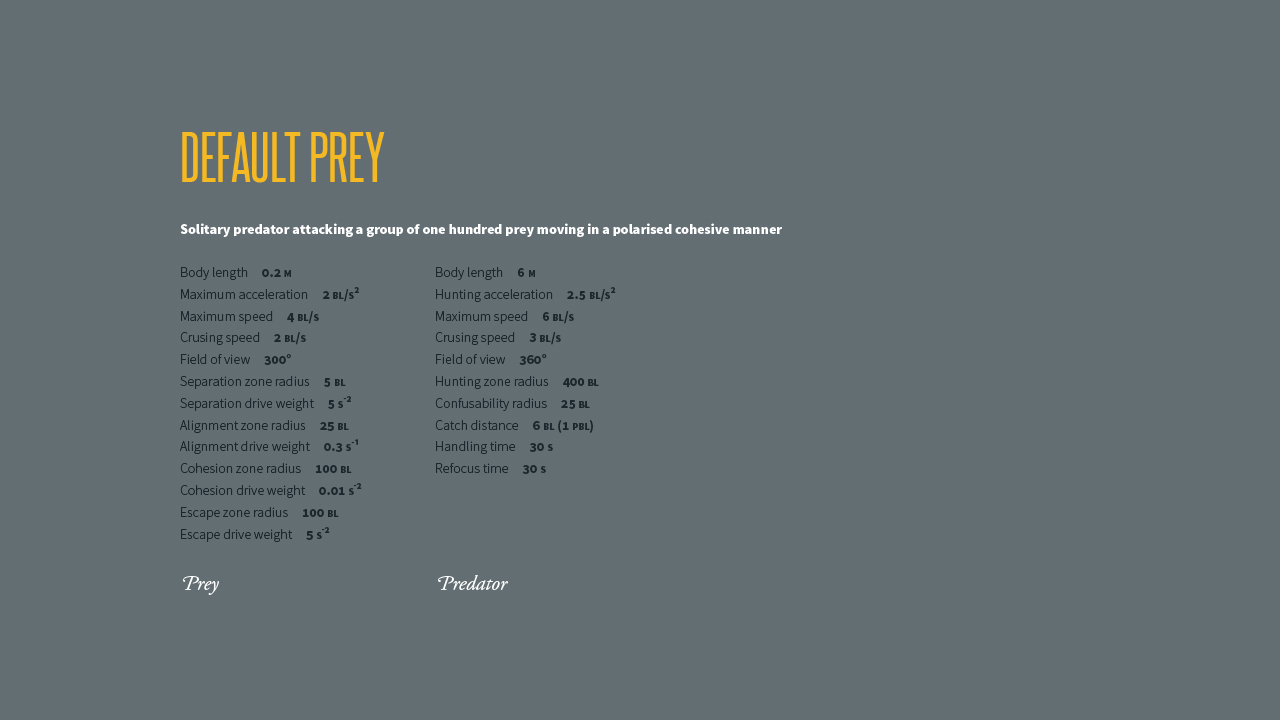
\includegraphics[width=\figurewidth]{ecomod/video_Default}
	\caption{Solitary predator attacking a group of one hundred prey moving in a polarised cohesive manner. Comparison between predator attack tactics: attacking a random prey, attacking the most central prey, attacking the nearest prey, attacking the most peripheral prey, mixture of simple tactics, dispersing tactic. Available online at \href{https://vimeo.com/119847644}{vimeo.com/119847644}.}
	\label{video:V1:ecomod}
\end{video}

\begin{video}[!hb] % force figure to appear on same page
	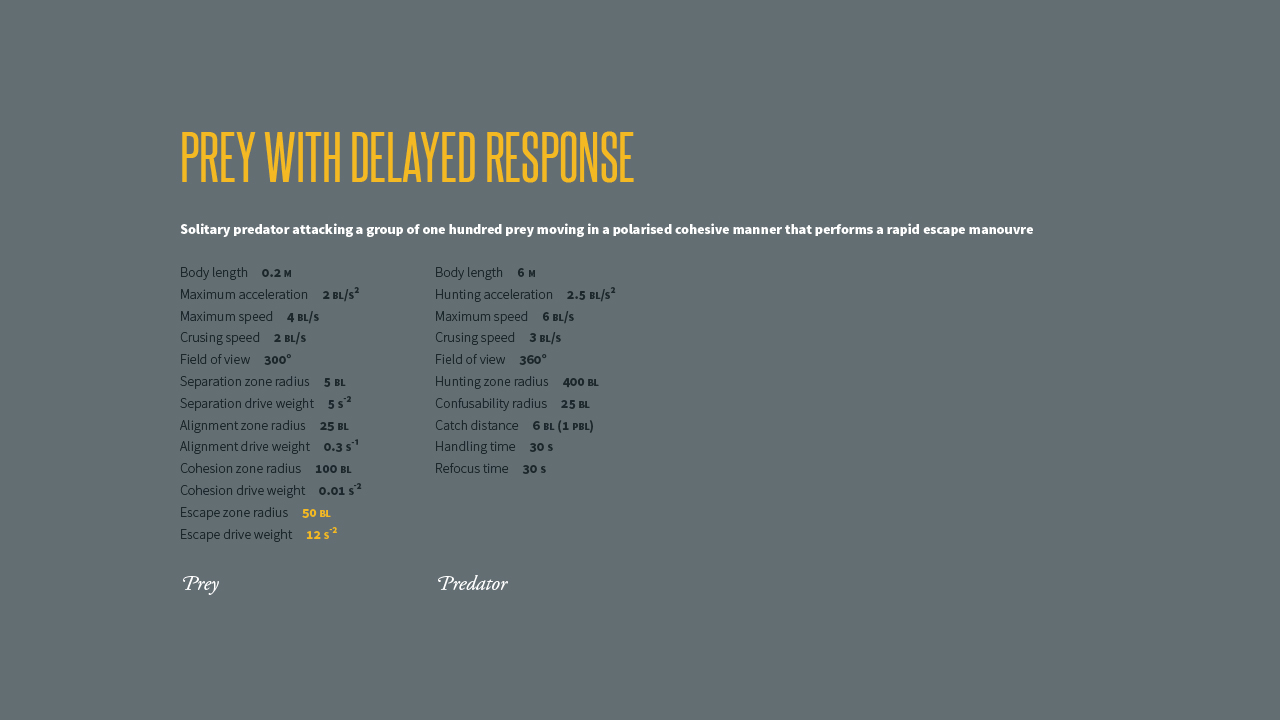
\includegraphics[width=\figurewidth]{ecomod/video_Delayed}
	\caption{Solitary predator attacking a group of one hundred prey moving in a polarised cohesive manner. Comparison between predator attack tactics for the case of prey with a delayed response: attacking a random prey, attacking the most central prey, attacking the nearest prey, attacking the most peripheral prey, mixture of simple tactics, dispersing tactic. Available online at \href{https://vimeo.com/119847316}{vimeo.com/119847316}.}
	\label{video:V2:ecomod}
\end{video}

\begin{video}[p]
	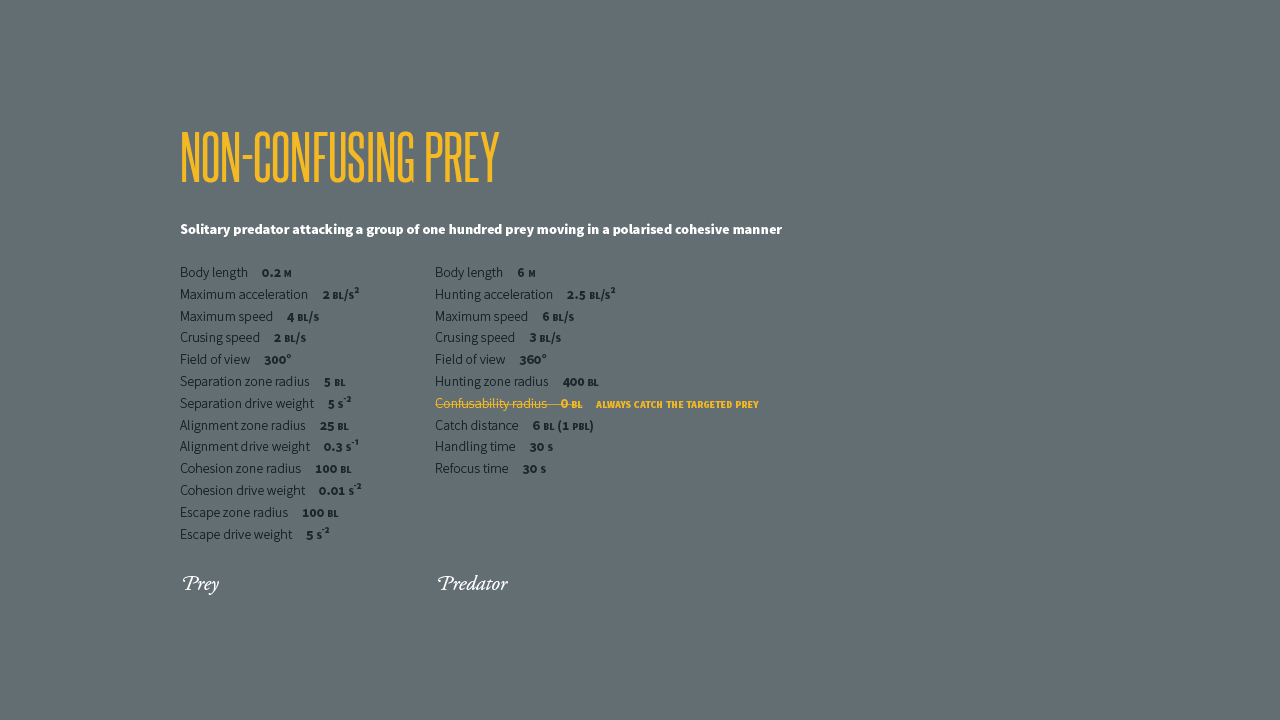
\includegraphics[width=\figurewidth]{ecomod/video_NC}
	\caption{Solitary predator attacking a group of one hundred prey moving in a polarised cohesive manner. Comparison between predator attack tactics for the case of non-confusing prey: attacking a random prey, attacking the most central prey, attacking the nearest prey, attacking the most peripheral prey, mixture of simple tactics, dispersing tactic. Available online at \href{https://vimeo.com/119846051}{vimeo.com/119846051}.}
	\label{video:V3:ecomod}
\end{video}

\end{subappendices}

	% !TeX root = ./thesis.tex










%==============================
\chapter[Evolution of collective behaviour in an artificial world\\ using linguistic fuzzy rule-based systems]{Evolution of\\ collective behaviour in an artificial world using linguistic fuzzy rule-based systems}
\chaptermark{Evolution of collective behaviour in a fuzzy artificial world} % change running head for chapter
\label{chap:plos}

\chapterAbstract[published={plos/Demsar_Lebar_Bajec_2017.pdf}]{Collective behaviour is a fascinating and easily observable phenomenon, attractive to a wide range of researchers. In biology, computational models have been extensively used to investigate various properties of collective behaviour, such as: transfer of information across the group, benefits of grouping (defence against predation, foraging), group decision–making process, and group behaviour types. The question ``why,'' however remains largely unanswered. Here the interest goes into which pressures led to the evolution of such behaviour, and evolutionary computational models have already been used to test various biological hypotheses. Most of these models use genetic algorithms to tune the parameters of previously presented non-evolutionary models, but very few attempt to evolve collective behaviour from scratch. Of these last, the successful attempts display clumping or swarming behaviour. Empirical evidence suggests that in fish schools there exist three classes of behaviour; swarming, milling and polarized. In this paper we present a novel, artificial life-like evolutionary model, where individual agents are governed by linguistic fuzzy rule-based systems, which is capable of evolving all three classes of behaviour.}

%-----
\section{Introduction}

The intricate patterns of collective motion, observable in flocks of birds, schools of fish, herds of ungulates, swarms of insects, and human crowds \cite{lebarbajec2009organized,silverberg2013collective,sumpter2006principles,vicsek2012collective} are a special treat. It is no wonder that the study of computational modelling of collective behaviour has a broad interdisciplinary appeal, more so as recent studies suggest similar patterns even in cancerous cells \cite{deisboeck2009collective}. Researchers come from various areas: ethology, biology, mathematics, physics, computer science and robotics/control theory.

The first attempts at modelling collective behaviour date to the early 1980s, when Aoki \cite{aoki1982simulation} and Okubo \cite{okubo1986dynamical} proposed an individual-based approach to the simulation of schooling mechanisms in fish, but it was Reynolds' 1987 seminal paper \cite{reynolds1987flocks} that attracted computer scientists to the field. Current models are presented by an interdisciplinary community and are either minimalistic with the goal of being as mathematically tractable as possible \cite{collignon2016stochastic,nagai2015collective,tanner2003fixed,tanner2003dynamic,toner1995longrange,vicsek1995novel}, or far more complex than the early ones \cite{couzin2002collective,demsar2014simulated,hemelrijk2008selforganized,hildenbrandt2010selforganized,pino2015modeling}. However, the basic principles have stayed the same for over 30 years of active research.

Nowadays, collective behaviour is normally modelled on a per individual basis, where one models a single individual and observes the emergent behaviour that arises when a number of these individuals interact, thus closely following Aristotle's concept of ``the whole is more than the sum of its parts.'' An individual is typically modelled as a multi-stage process \cite{lebarbajec2007boids,fine2013unifying}, in the minimal form consisting of perception, drives and action selection. Perception mimics the animal's act of filtering out only the most important information about the surrounding environment (in most cases this is a subset of position and orientation data about nearby neighbours). Drives reproduce the modelled animal's needs, where (with the notable exception of the most minimalistic models) these are typically the animal's tendency to a) avoid collisions with nearby neighbours, termed separation, b) to surround itself with neighbours, termed cohesion, and c) to align in speed and velocity with neighbours, termed alignment. As the drives are potentially contradictory, \eg separation and cohesion, the third stage, action selection, is responsible for devising the final action of the modelled animal, typically a change in heading and/or speed. Most of the models encode the drives by means of equations, where for example cohesion is typically encoded as a force vector directing the individual towards the centroid of nearby neighbours \cite{vicsek2012collective,lebarbajec2009organized}. Action selection is then most often a weighed sum of force vectors; actions that would fulfil individual drives.

A review of biological literature suggests that in view of encoding the animal's drives not much has changed since the early days, whereas a lot of research has been devoted to perception and interaction. All because it is still not completely known ``how'' when a flock of tens of thousands individuals is turning and wheeling it seems that all turn at once, reminiscent of ``thought transference'' or ``telepathy'' \cite{lebarbajec2009organized,hayes2011flights}. Ballerini\etal \cite{ballerini2008interaction} based on \textsc{3d} data collected from live flocks of birds argued that interaction is not metric, \ie distance limited, as in \cite{reynolds1987flocks}, but rather topological, \ie number limited. While some earlier studies proposed a zone based interaction \cite{couzin2002collective,couzin2005effective} and later studies investigated the effects of visual occlusion \cite{demsar2014simulated,kunz2012simulations,pearce2014role} current research suggests that one can reproduce empirical data from physicists in Rome \cite{ballerini2008interaction,cavagna2013diffusion} if either a) one assumes the probability of interaction between two individuals is inversely proportional to their distance \cite{bode2011limited}, or b) one assumes that individual birds avoid a single closest neighbour only and they align with and are attracted to their seven closest neighbours \cite{hemelrijk2015diffusion}, as assumed in Ballerini\etal \cite{ballerini2008interaction}.

The use of fuzzy logic as the means of encoding the simulated animal's drives was first proposed in \cite{lebarbajec2003boids,lebarbajec2003fuzzifying,lebarbajec2005fuzzy,lebarbajec2005simulating} and later followed by others \cite{dong2013fuzzy,gu2008using,lee2011design,sahu2013fuzzy,tron2004mathematical,wang2007behaviour,yu2010control,yu2010obstacle}. While with the premise of easing the construction of new, yet unknown, drives to ethologists the first studies proposed a linguistic fuzzy rule-based system the later ones were more control centric and most of them proposed a Takagi-Sugeno rule base. A linguistic fuzzy rule-base was used also in \cite{sahu2013fuzzy} and \cite{lee2011design}, but contrary to \cite{lebarbajec2005simulating} where a) the drives are encoded indirectly, b) no-uncertainty is assumed and c) collective behaviour emerges with no designated leader, \cite{sahu2013fuzzy} was based on the leader-follower concept and \cite{lee2011design} while concentrating on noisy sensor measurements presented an interval-valued fuzzy controller.

Some researchers from the artificial life community might argue that most of the aforementioned models are in essence top-down models of collective behaviour in that their drives were designed by observing high-level behaviours of the group, regardless if these same drives dictate the behaviour of the individuals in the group. For a true bottom-up model then, where the individuals have their own individual movement rules that ``may'' lead to collective behaviour when simulated, one would need to investigate the evolution of an individuals' movement rules. Indeed, regardless of all research that has been done the biological question ``why'' collective behaviour evolved still remains largely unanswered. Here the interest goes more into which pressures have led to the evolution of collective animal behaviour. From the early days of research in the field several studies attempted the evolution of collective behaviour. The methods range from genetic programming with \textsc{lisp} \cite{reynolds1993evolved}, \textsc{push} \cite{spector2005emergence}, neuroevolution \cite{kwasnicka2011flocking,ward2001evolving,zaera1996not} to evolutionary optimization of the complete sensory-motor flow via Kuramoto oscillators bound to a synthetic optic flow retina \cite{pino2015modeling}. These studies were mostly concerned if an evolutionary computation system can be used to evolve collective behaviour from scratch and had various degrees of success, where the latter can most often be attributed to steered evolution. More recently evolutionary models are being used to test the biological hypothesis that collective behaviour evolved due to combined search for food resources \cite{witkowski2016emergence}, or as protection from predation \cite{oboshi2003collective}, which can be split further by the key ideas; selfish herd \cite{hamilton1971geometry,morrell2015consequences,olson2013critical,olson2016evolution,reluga2005simulated,wood2007evolving}, predator confusion \cite{chen2014minimal,kunz2006prey,nishimura1997emergence,olson2013predator,zheng2005behavior}, many eyes \cite{ruxton2008application,olson2015exploring}, and dilution of risk \cite{tosh2011conditions}. Most of the aforementioned evolutionary models use genetic algorithms to tune a) the importance of known drives (cohesion, separation, alignment) and/or additional drives (\eg escape), and/or b) model parameters (field of view, escape distance, etc.). Very few studies attempted and successfully evolved collective behaviour from scratch, and in these cases the evolved behaviour can be termed as ``crude''; portraying only clumping \cite{biswas2014causes,witkowski2016emergence}, or swarming with collisions \cite{olson2013critical,olson2013predator,olson2016evolution,witkowski2016emergence}.

In this paper we present an evolutionary model where the drives are encoded by means of linguistic fuzzy rule-based systems and is capable of evolving more ``refined'' behaviours.

%-----
\section{Materials and Methods}

Our model is an individual-based model consisting of predator and prey agents that coexist in a \textsc{2d} environment (artificial world). The simulation runs at discrete updates, where each individual agent (predator or prey) based on the perceived state of the environment computes its drives, and with respect to the desired change in speed and heading updates its velocity and position \cite{lebarbajec2005fuzzy,lebarbajec2005simulating}. For the sake of simplicity the time steps and distances in the simulations are given in arbitrary units, have no physical meaning and are used for comparative purposes only. To keep the model's complexity as low as possible we also assume constant, but different speeds for predator and prey agents. The following sections provide more details about the implementation of the predator and prey agents, as well as specifics about the evolutionary process.

%-----
\subsection{The predator agent}

Since some avian visual sit-and-wait predators scan the neighbourhood by turning their head \cite{gall2010visual,orourke2010hawkeyes2} and some aquatic predators perform area-restricted search \cite{thums2011insitu}, our predator agents are capable of perceiving prey agents regardless of their relative bearing. For simplicity reasons, perception is limited only by distance, \ie we also do not consider visual occlusion. Following our previous research \cite{demsar2014simulated} the predator agent's drives for target prey pursuit are encoded by means of a linguistic fuzzy rule-based system and pre-set, \ie excluded from evolution.

The goal of predator agents is to capture prey agents. We let multiple predator agents coexist, as recent studies suggest that the cumulative effect of high frequency attacks (through disorganisation of school cohesiveness) may increase the feeding success of each individual \cite{lett2014effects,thiebault2015howto}. Individual predator agents enter the artificial world after an initial random interval of update steps (\emph{re-enter time}). Each predator agent continuously attacks prey agents for \emph{hunt duration} update steps, then they are removed from the environment and a new predator agent enters after a random interval of update steps (\emph{re-enter time}). Predator agents appear at random locations that are \emph{ambush distance} from the artificial world centre, with their initial heading towards the centre. An attack involves target-selection, pursuit and capture attempt.

\begin{table}
  \caption{Predator agent parameter values.}
  \label{tab:predator}
  \begin{tabular}{lll}
    \toprule
    Description & Value \\
    \midrule
    number of predator agents & 16 \\
    ambush distance & 400 \\
    re-enter time (update steps) & 600--\num{1200} \\
    hunt duration (update steps) & 600 \\
    \hdashline
    type & \ST predator & \HDA predator \\
    size & 6 & 12\\
    speed & 3 & \num{1.5}\\
    perception distance & 500 & 500 \\
    catch distance & 6 & 12\\
    \bottomrule
  \end{tabular}
\end{table}

Following previous research \cite{demsar2014simulated,demsar2015simulating,olson2016evolution} we implemented four target-selection tactics; attack the nearest prey agent, attack the most isolated prey agent, attack the most central prey agent, and high density area attack. Predators that attack the nearest, most isolated or most central prey individual, focus their attention on a single member of the prey group (\ST), \ie they select a single prey agent as target, and pursue it until captured. Predators that attack high density areas are larger than a single prey individual and do not select as target, pursue, and capture a single prey individual, but can capture several prey individuals in a single predation event. In view of recent results that attribute the evolution of clumping to the dilution of risk \cite{biswas2014causes} rather than predator confusion \cite{olson2013predator}, we opted to model our agents as non-confusable. This served also not to overly promote collective behaviour, as one could argue that outside attacks on the nearest or most isolated prey individual in combination with confusion pressures prey into grouping and thus might be viewed as a form of steered evolution. Additionally, if from an evolutionary perspective outside attacks on the nearest or most isolated prey individual have a positive influence on grouping, attacks on the most central prey individual or high density area attacks (\HDA) should have a negative one \cite{olson2016evolution}. Since our primary interest was the discovery of a wide variety of behaviours, we for this reason let the specific tactic an individual predator agent uses be chosen randomly (uniform probability). The complete set of predator agent parameters can be viewed in \tablename~\ref{tab:predator}.

%-----
\subsection{The prey agent}

Similar to predator agents, the prey agent's perception is limited by distance only, \ie we ignore the visual field blind area and visual occlusion. However, following recent research on perception models capable of reproducing empirical data \cite{bode2011limited,hemelrijk2015diffusion} we chose to model the probability of interaction between two prey agents as inversely proportional to their distance. Since every individual prey agent's drives are encoded by means of a linguistic fuzzy rule-based system and evolve through time, the approach goes also in our favour as it reduces the number of rules that have to be evaluated per agent.

\begin{table}
  \caption{Prey agent parameter values.}
  \label{tab:prey}
  \begin{tabular}{ll}
    \toprule
    Description & Value \\
    \midrule
    number of prey agents & 100 \\
    spawn area radius & 325 \\
    living area side length & 375 \\
    \hdashline
    size & 1 \\
    speed & 2 \\
    perception distance & 100 \\
    \hdashline
    initial energy & \num{1000} \\
    foraging gain & 1 \\
    collision penalty & \num{-10} \\
    wandering penalty & \num{-10} \\
    \bottomrule
  \end{tabular}
\end{table}

The goal of prey agents is to live as long as possible in the artificial world. When born, a prey agent is assigned a specific amount of \emph{initial energy} (see \tablename~\ref{tab:prey}) and on every update step it is rewarded for ``living'' (\emph{foraging gain}). Prey agents that collide or wander outside a square living area are penalized with a reduction of energy. One could argue that the \emph{wandering penalty} is a form of steered evolution, but the \emph{living area side length} was set to a large enough size that this does not overly promote grouping behaviour (see \figurename~\ref{figC1} and \videoname~\ref{video:V1:plos}). The living area represents an area rich with food, shelter, or in another sense, attractive area. In our model the only purpose of this area is to keep prey agents inside a limited area of the artificial world, which could be achieved also by using periodic boundary conditions to create an infinite lattice, but we opted for an approach where prey agents learn to keep within the restricted area themselves.

A prey agent dies when its energy drops to 0 or is caught by a predator agent. When a prey agent dies it is removed from the environment and a new prey agent is created, so that the group of ``live'' prey agents is kept constant through time. The new prey agent, initially heading in a random direction, appears at a random location on a closed disc centred to the living area (\emph{spawn area}). The linguistic rule base of the new prey agent is subject to evolution via crossover and mutation (see Evolutionary process).

\begin{table}
  \caption{Prey agent fuzzy data base.}
  \label{tab:preyDB}
  \begin{tabular}{lllp{2.7cm}}
    \toprule
    & Linguistic variable & Linguistic value & Triangular\newline fuzzy number \\
    \midrule
    interaction & distance & next & $\left<0,0,10\right>$ \\
    & & close & $\left<0,15,40\right>$ \\
    & & near & $\left<20,40,60\right>$ \\
    & & away & $\left<50,60,100\right>$ \\
    & & far & $\left<60,100,100\right>$ \\
    & relative bearing & left & $\left<-180,-90,0\right>$ \\
    & & in front & $\left<-90,0,90\right>$ \\
    & & right & $\left<0,90,180\right>$ \\
    & & behind & $\left<90,180,-90\right>_{360}$ \\
    & relative heading & left & $\left<-180,-90,0\right>$ \\
    & & same & $\left<-90,0,90\right>$ \\
    & & right & $\left<0,90,180\right>$ \\
    & & opposite & $\left<90,180,-90\right>_{360}$ \\
    \hdashline
    living area & distance & next & $\left<0,0,10\right>$ \\
    & & close & $\left<0,15,40\right>$ \\
    & & near & $\left<20,40,60\right>$ \\
    & & away & $\left<50,60,100\right>$ \\
    & & far & $\left<60,100,100\right>$ \\
    & relative bearing & left & $\left<-180,-90,0\right>$ \\
    & & in front & $\left<-90,0,90\right>$ \\
    & & right & $\left<0,90,180\right>$ \\
    & & behind & $\left<90,180,-90\right>_{360}$ \\
    \hdashline
    action & heading change & hard left & $\left<-180,-180,-90\right>$ \\
    & & left & $\left<-180,-90,0\right>$ \\
    & & none & $\left<-90,0,90\right>$ \\
    & & right & $\left<0,90,180\right>$ \\
    & & hard right & $\left<90,180,180\right>$ \\
    \bottomrule
  \end{tabular}
\end{table}

The prey agent is capable of perceiving a) the distance, relative bearing, and relative heading of the interacting prey individual, b) the distance, relative bearing, and relative heading of the nearest predator, as well as c) the distance and relative bearing to the closest point on the square that represents the outside edge of the living area. We assume no uncertainty in the data and model all inputs as singleton fuzzy values \cite{mendel2001uncertain}. If either all other prey individuals, predators, or living area borders are outside of the prey agent's perception distance, the corresponding linguistic variables are set to \textsc{null}, so that none of the fuzzy rules that contain the variable as part of the premise fire. In fuzzy reasoning (see \figurename~\ref{fig1}) we use the \emph{product} t-norm for conjunction and implication, aggregate rules via the \emph{probabilistic sum} s-norm, and compute the crisp output (desired change in heading) by means of the \emph{centre-of-gravity} defuzzification method. The linguistic variables (\tablename~\ref{tab:preyDB}) are decomposed into linguistic values, which are defined as either triangular fuzzy numbers
%
\begin{equation}
\mu(x)=\left<l,m,r\right>=\max{\left(\min\left(\frac{x-l}{m-l}, \frac{r-x}{r-m}\right),0\right)},
\end{equation}
%
or periodic triangular fuzzy numbers
%
\begin{equation}
\mu(x)=\left<l,m,r\right>_c=\max\left(\min\left(\frac{(x-l) \bmod c}{(m-l) \bmod c}, \frac{(r-x) \bmod c}{(r-m) \bmod c}\right),0\right).
\end{equation}

\begin{figure}
  \includegraphics[width=\figurewidth]{plos/fig1}
  \infigurecaption{Section A shows the current state of the artificial world. The observed prey agent is depicted in black and the nearest predator in red. In this simplified example the observed prey agent performs fuzzy reasoning solely based on the nearest predator's relative bearing (in this case \ang{-126}). The left part of section B presents the evaluation of the degree of truth of the antecedents of individual if-then rules that are listed at the bottom of this section. We assume no uncertainty in the data and model all inputs as singleton fuzzy values. For example, the degree of truth of the antecedent ``nearest predator relative bearing is left'' is therefore computed as $\left<\text{\num{-180}},\text{\num{-90}},\text{\num{0}}\right>(\text{\num{-126}}) = \text{\num{0.6}}$. The right part of section B presents fuzzy inference or the evaluation of the consequent part of individual rules. Since we use the \emph{product} t-norm ($\symsfit{x \circ y=xy}$) for implication this translates to scaling the triangular fuzzy number that is used to define the corresponding output linguistic variable's value (shaded areas). For example, in the case of consequent ``heading change is right,'' this means $\text{\num{0.6}} \circ \left<\text{\num{0}},\text{\num{90}},\text{\num{180}}\right>$. Section C presents the aggregation of individual consequent parts and based on that the computation of the final, crisp output, the conclusion (desired change in heading). We aggregate rules via the \emph{probabilistic sum} s-norm ($\symsfit{x \diamond y=x+y-xy}$), and compute the crisp output by means of the \emph{centre-of-gravity} defuzzification method. This means that the shaded area in section C (aggregated shaded areas from section B) gets translated into \num{54.375}, the desired change in heading for the observed prey agent in this simplified example. For further details on fuzzy reasoning in general and its application to the modelling of collective behaviour consult \cite{mendel2001uncertain,lebarbajec2003boids,lebarbajec2003fuzzifying,lebarbajec2005fuzzy,lebarbajec2005simulating}.}
  \caption{A simplified example of fuzzy reasoning.}
  \label{fig1}
\end{figure}

%-----
\subsection{Evolutionary process}

Genetic algorithms have a long history in providing learning and adaptation capabilities to fuzzy rule-based systems \cite{herrera2008genetic,fazzolari2013review}. While in most applications the desired outcome of the evolutionary process is a better, faster, more accurate or interpretable rule-based system \cite{casillias2003accuracy,casillias2003interpretability,cordon2011historical} in our case the goal of the evolutionary process is discovery through exploration. In other words the only objective considered by our fitness function is the survivability of prey agents, assessed via their energy level and therefore the fitness function does not consider collective behaviour directly.

In our artificial world predator and prey agents coexist and the goal of predator agents is to capture prey agents, while the goal of prey agents is to survive. The direct competition of individual prey agents by way of their drives (\ie rules of motion encoded via a linguistic fuzzy rule-based system) will lead to the emergence of collective behaviour only if such behaviour helps individual prey agents to ``live'' longer. Artificial life based evolutionary computation like this tries to mimic open-ended evolution \cite{aguilar2014thepast,mitchell1994genetic,soros2014identifying}. To our knowledge there have been only few similar evolutionary fuzzy systems \cite{barriosrolania2015bacterially,halavati2005fuzzy} and none devoted to the evolution of collective behaviour.

As we wished to focus on human interpretable rules and keep the complexity as low as possible, we opted to use a fixed data base and evolve only the rule base \cite{cordon2004ten}. In addition, as the order of importance of individual inputs is unknown, we allowed for incomplete rule sets, \ie we limited only the number of rules in the rule base as well as the number of antecedents per individual rule.

To recapitulate, prey agent behaviour was evolved via an open-ended like evolution where the behaviour of an individual prey agent is defined by the complete fuzzy rule base with a variable-length (messy) coding scheme \cite{hoffman1997evolutionary}. The chromosome of each individual was thus its set of rules, in genetic fuzzy systems labeled as the Pittsburg approach \cite{herrera2008genetic}. Individual prey agents of the initial population were assigned random behaviours (\ie a set of random fuzzy rules). They were placed at random locations on a closed disc centred to the living area and assigned random headings. When a prey agent was caught by a predator agent or died due to numerous collisions or wanderings outside of the living area, it was removed and a new prey agent was created. Two ``live'' prey agents were chosen as its parents, where selection was fitness-proportional. The fuzzy rule base of the new prey agent was constructed by first choosing a random rule base length, and then randomly selecting individual rules from the joint sets of its parents' rules. Following that, a mutation could occur; it triggered either an addition of new totally random rules or removal of existing rules from the new prey agent's rule base.

\begin{table}
  \caption{Evolutionary process parameter values.}
  \label{tab:GA}
  \begin{tabular}{ll}
    \toprule
    Description & Value \\
    \midrule
    number of evolutions & 20 \\
    total length (update steps) & \num{10000000} \\
    rule base upper bound & 50 \\
    antecedents upper bound & 4 \\
    mutation probability & 2\% \\
    upper bound of add rules mutation & 3 \\
    upper bound of remove rules mutation & 3 \\
    \bottomrule
  \end{tabular}
\end{table}

%-----
\section{Results and discussion}

We performed 20 individual evolutionary runs (\tablename~\ref{tab:GA}). Each evolved behaviour was then evaluated by running 20 replicates of a separate simulation (\tablename~\ref{tab:EVA}). In this simulation, prey agents were initially placed at random locations on a closed disc centred to the living area and assigned random headings. After an initial stabilisation period, the observed parameters were first recorded without the presence of predators; only then a predator was introduced and another set of observed parameters was recorded.

\begin{table}
  \caption{Validation process parameter values.}
  \label{tab:EVA}
  \begin{tabular}{ll}
    \toprule
    Description & Value \\
    \midrule
    replicates of validation & 20 \\
    stabilisation period (update steps) & 900 \\
    predator introduction (update step) & \num{1800} \\
    total length (update steps) & \num{3600} \\
    \bottomrule
  \end{tabular}
\end{table}

%-----
\subsection{Behaviour analysis}

For the analysis of the evolved behaviour we resorted to both visual inspection \cite{kunz2006prey} and biologically relevant observables. Here we concentrated on local density \cite{huepe2008newtools}, number of groups \cite{lebarbajec2007boids,viscido2015using}, polarization and rotation \cite{couzin2002collective,tunstrom2013collective,vicsek2012collective}. Polarization
%
\begin{equation}
p=\frac{1}{n}\left|\sum_{i=1}^{n}\uvec{v}_i\right|,
\end{equation}
%
where $n$ is the number of agents and $\uvec{v}_i$ is the unit direction vector of agent $i$, provides a measure of how aligned the individuals in a group are. Rotation
%
\begin{equation}
m=\frac{1}{n}\left|\sum_{i=1}^{n}\uvec{c}_{i} \times \uvec{v}_i\right|,
\end{equation}
%
where $\uvec{c}_i$ is the position of agent $i$ in the local coordinate frame of the group, on the other hand, expresses the degree of rotation of the group about its centre. Polarization and rotation were computed on the local scale, \ie considering only prey agents that are part of the same group, as well as on the global scale, \ie considering all prey agents as being part of one single group. Groups were established based on potential interaction (direct or indirect) \cite{lebarbajec2007boids,viscido2015using}. In other words, for an observed prey agent, all prey individuals that were inside its perception distance were considered as being part of its group, as well as, recursively all prey individuals that were inside the perception distance of any of this group's members. Prey agents that had all prey individuals outside their perception distance were marked as stragglers and excluded from the analysis on the local scale (see \figurename~\ref{fig2}).

\begin{figure}
  \includegraphics[width=\figurewidth]{plos/fig2}
  \infigurecaption{Presented are two groups (one in a milling state, green shading, and one in a polar state, blue shading) and one straggler (a prey agent that can neither influence nor be influenced by any other prey individual, grey shading).}
  \caption{Prey agents that can influence each other either directly or indirectly via others are considered as being part of the same group.}
  \label{fig2}
\end{figure}

As based on the relation between polarization and rotation Couzin\etal \cite{couzin2002collective} defined four classes of collective behaviour, namely \emph{swarming}, \emph{milling}, \emph{dynamic parallel group} and \emph{highly parallel group} we, in addition to assessing the behaviour visually, also classify it based on the corresponding representative values of polarization and rotation. Here we followed recent research by Tunstrøm\etal \cite{tunstrom2013collective}, who defined that a group is in: the polar state (P) when polarization \textgreater\,\num{0.65} and rotation \textless\,\num{0.35}; the milling state (M) when polarization \textless\,\num{0.35} and rotation \textgreater\,\num{0.65}; and the swarm state (S) when polarization \textless\,\num{0.35} and rotation \textless\,\num{0.35}. Outside these ranges it is said to be in transition (T).

As it can be seen in \figurename~\ref{fig3}, all 20 evolutions led to an increase in local density. Overall the mean local density at update step 0 was \num{14.07} \ci{13.87}{14.26}, and the average local density during update steps \numrange{900}{1800} was \num{42.47} \ci{40.91}{44.1}. It ranged from \num{17.74} \ci{16.46}{19.18} in the case of evolution no. 11, to \num{72.47} \ci{67.85}{77.36} in the case of evolution no. 5. In all cases the increase was statistically significant ($p$\,\textless\,\num{0.0001}). The overall average number of groups during update steps \numrange{900}{1800} was \num{2.762} \ci{2.603}{2.932}, and ranged from \num{1.001} \ci{1}{1.002} in the case of evolution no. 12 to \num{5.743} \ci{5.374}{6.122} in the case of evolution no. 14.

\begin{figure}
  \includegraphics[width=\figurewidth]{plos/fig3}
  \infigurecaption{The left graph displays the mean and bootstrapped 95\%~\CI of the local density at update step 0, as well as, mean and bootstrap 95\%~\CI of the average local density during update steps \numrange{900}{1800}. The middle graph displays the mean and bootstrapped 95\%~\CI of the number of groups at update step 0 and the mean and bootstrapped 95\%~\CI of the average number of groups during update steps \numrange{900}{1800}. The right graph shows the cumulative proportion of time spent in a specific collective state. The number of replicates was 20. Evolution ids were sorted based on the average local density during update steps \numrange{900}{1800}. Ids marked in bold correspond to representatives of the four classes of evolved behaviour (see main text for details).}
  \caption{Local density, number of groups, and time spent in a specific collective state for each evolutionary run.}
  \label{fig3}
\end{figure}

The proportion of time spent in a specific collective state (P, M, S, T) was determined by counting the cumulative number of update steps over all 20 replicates that individual groups spent in a specific state. When there was more than one group, each group's state was allocated a corresponding proportion of update steps, \eg when there were three groups in one step their respective states were assigned one third of the update step each. Based on the state in which the largest proportion of time was spent in, the evolved behaviours were classified as: polarized (evolutions no. 2, 11, 12, 17 and 20), milling (evolutions no. 5--9, 13--16, 18, and 19), and swarming (evolution no. 4). Evolutions no. 1, 3 and 10 spent the largest proportion of time in transition between states. This was confirmed through visual inspection. As we also noticed that the groups continuously transitioned between different states (polarized-milling-swarming), a characteristic associated with schooling fish (golden shiner, \emph{Notemigonus crysoleucas}) \cite{tunstrom2013collective}, we classified this type of evolved behaviour as \emph{dynamic} (D). \figurename~\ref{fig4} shows representative time series of global polarization and rotation for each of the four types of evolved behaviour. Evolutions no. 12, 6, 4 and 10 were selected based on high mean local density and low mean number of groups (marked as bold in \figurename~\ref{fig3}).

\begin{figure}
  \includegraphics[width=\figurewidth]{plos/fig4}
  \infigurecaption{Evolutions no. 12, 6, 4 and 10 (marked as bold in \figurename~\ref{fig3}) were selected as representatives of polarized, milling, swarming and dynamic behaviour based on the proportion of time spent in a specific state, high mean local density and low mean number of groups. For video sequences of the representative evolved behaviours see Videos~\ref{video:V2:plos}--\ref{video:V6:plos}.}
  \caption{Time series of global polarization and rotation for each of the four classes of evolved behaviour.}
  \label{fig4}
\end{figure}
%\FloatBarrier
To gain further understanding of the evolved behaviour in the case of evolution no. 10, we performed an experiment similar to the one Tunstrøm\etal \cite[\figurename~3]{tunstrom2013collective} used to evaluate the relationship between group size and behaviour stability. Note that a) in our case the speed was not varied, but kept constant (see \tablename~\ref{tab:prey}), b) in our case there was a boundary interaction (living area), c) global polarization and rotation were recorded during update steps \numrange{900}{1800}, e) 20 replicates were performed, and d) the rule bases of the 30, 70, 150, 300 agents were on each replicate chosen randomly from the pool of 100 rule bases that resulted from evolution no. 10. The density plot in \figurename~\ref{fig5} shows qualitatively similar results to those presented by Tunstrøm\etal \cite[\figurename~2]{tunstrom2013collective}. With increasing the number of agents, the global behaviour changes from predominately polarized to predominately milling. In addition, visual inspection revealed that, like in the case of schooling fish \cite[\figurename~6]{tunstrom2013collective}, transitions from polarized to the milling state and back were initiated mainly by a) interaction with the living area boundary or b) agents located in the frontal region of the group, which after a turn spotted the back of the group (see \videoname~\ref{video:V6:plos}).

\begin{figure}
  \includegraphics[width=\figurewidth]{plos/fig5}
  \infigurecaption{The density plots visualize the relationship between group size and behaviour stability. Increasing the number of agents leads global behaviour to change from predominantly polarized to predominantly milling.}
  \caption{Density plot of global polarization versus rotation for various group sizes in the case of evolution no.~10.}
  \label{fig5}
\end{figure}

A Wilcoxon Signed-Ranks Test was used to compare the local density and number of groups during update steps \numrange{1800}{3600}, in which the predator was not present, to the local density and number of groups during these update steps in which the predator was present. With the exception of evolution no. 3, the presence of a predator caused a statistically significant ($p$\,\textless\,\num{0.01}) change in local prey density and the number of groups. An increase in local density in combination with a decrease in the number of groups was seen in evolutions no. 1, 10 and 11. A decrease in local density in combination with an increase in number of groups was seen in evolutions no. 2, 4, 5, 7, 9, 12, 13, 16, 17, 19. A decrease in both local density and number of groups was noted in evolutions no. 6, 14, 15, 18 and 20. Finally, an increase in both local density and number of groups occurred in the case of evolution no. 8. In the case of evolution no. 3 no significant difference was observed in both local density (\Ztest{-0.786}{0.432}) and the number of groups (\Ztest{-1.645}{0.1}). Visual inspection revealed that even in the case of evolution no. 3 individual prey agents did react to predators by turning away from it, however this had no notable effect on local density or the number of groups.

%-----
\subsection{Rule base analysis}

Since in our case the data base was fixed, the evolved rule bases were summarized by means of six parameters, namely \emph{living area}, \emph{predator}, \emph{prey}, \emph{specificity}, \emph{bias}, and \emph{size}. The first three were computed as the average proportion of rule antecedents that contain linguistic variables related to the living area, nearest predator, and interacting individual, respectively:
%
\begin{equation}
\rho^\alpha=\frac{1}{n}\sum_{i=1}^{n} \frac{a^\alpha_i}{a_i},
\end{equation}
%
where $n$ is the number of rules in the rule base, $a_i$ the number of antecedents in rule $i$, $\alpha$ either living area, nearest predator, or interacting individual, and $a_i^\alpha$ the number of antecedents in rule $i$ that contain linguistic variables related to $\alpha$. These three parameters provide a rough approximation of the amount of attention the prey agent gives to a specific aspect of the artificial world. The parameters sum to 1. Since the living area is described with two linguistic variables, and the nearest predator and the interacting individual are with three, an equal attention to all three aspects would result in their values being 2/8, and 3/8, respectively.

Rule base specificity was determined as:
%
\begin{equation}
\varsigma = \frac{1}{n}\sum_{i=1}^{n} \frac{a_i-1}{m-1},
\end{equation}
%
where $n$ is the number of rules, $m$ the maximum number of antecedents (antecedents upper bound in \tablename~\ref{tab:GA}), and $a_i$ the number of antecedents in rule $i$. A value of 0 indicates all rules in the rule base use only one antecedent, thus individual rules are very general as the outcome is determined by a single input only. A value of 1, on the other hand, indicates that all rules in the rule base use the maximum number of antecedents, thus individual rules are highly specific as the outcome is determined by the highest number of inputs.

Bias provides a rough approximation of the prey agent turning side preference. It was computed as:
%
\begin{equation}
\beta = \frac{1}{2n}\sum_{i=1}^{n} 1+\frac{o_i}{180},
\end{equation}
%
where $n$ is the number of rules, and $o_i$ is the centroid of the output linguistic value of rule $i$. Values below \num{0.5} thus indicate a bias towards left turns, and values above \num{0.5} a bias towards right turns. Last but not least, size is simply the number of rules in the rule base divided by the maximum number of rules possible (rule base upper bound in \tablename~\ref{tab:GA}).

We first noted that overall prey agents based their decisions more on predator related linguistic variables (\Mdn{0.385}) than interacting individual related ones (\Mdn{0.361}; \Ztest[\textless]{19.591}{0.0001}). The amount of attention given to the living area (\Mdn{0.255}) was significantly different (\Ztest{-3.885}{1.025e-4}) than what would be expected if an equal attention was given to all three aspects of the artificial world. Similarly, a slight preference for turning to the right is present (\Mdn{0.507}; \Ztest[\textless]{-8.796}{0.0001}).

The evolved rule bases of individual evolutions were then grouped based on the type of evolved behaviour (polarized, milling, swarming, or dynamic) and a pairwise multiple comparison was made using a Benjamini-Yekutieli adjusted Dunn test. \figurename~\ref{fig6} shows box plots of the distributions of all six parameters, and statistical significance of the inter group differences.

\begin{figure}
  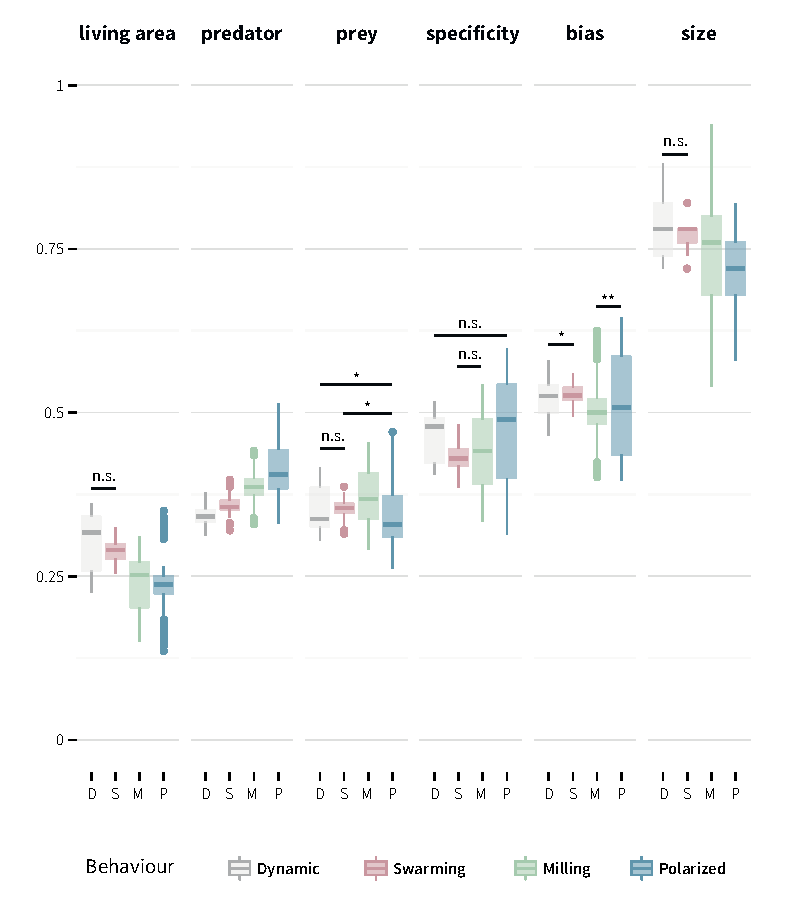
\includegraphics[width=\figurewidth]{plos/fig6}
  \infigurecaption{Grouping was based on the evolved behaviour class. Statistical significance of differences was obtained by means of a Benjamini-Yekutieli adjusted Dunn test. Symbols ns, * and ** indicate \textit{p}\,$\geq$\,\num{0.05}, \textit{p}\,\textless\,\num{0.05}, and \textit{p}\,\textless\,\num{0.01}, respectively. Unmarked cases denote significance at \textit{p}\,\textless\,\num{0.001}.}
  \caption{Box plots of the distributions of the six parameters through which the evolved rule sets were summarized.}
  \label{fig6}
\end{figure}

In the pairwise comparison between all four groups a difference at $p$\,\textless\,\num{0.001} was observed only in the case of the average proportion of rule antecedents that contain predator related linguistic variables. Interestingly non significant differences were observed between the dynamic and swarming group in the cases of a) the average proportion of rule antecedents that contain living area related linguistic variables, b) the average proportion of rule antecedents that contain linguistic variables related to the interacting individual, and c) rule base size. In the case of rule base specificity no statistically significant difference was observed between a) the dynamic and polarized group, and b) the swarming and milling group. The dynamic and swarming group had a significantly higher bias (\Mdn{0.526}) than the polarized (\Mdn{0.508}) and milling group (\Mdn{0.5}). Surprisingly, in the case of the milling group, the median rank was not statistically different than \num{0.5} (\Ztest{-1.919}{0.055}), which indicates no preference for the side of turning.

%-----
\section{Conclusion}

The study of collective behaviour has a broad interdisciplinary appeal. Numerous studies have attempted to evolve collective behaviour, most by tuning parameters of previously presented non-evolutionary models. Very few succeeded to evolve it from scratch, and even in these cases the evolved behaviour can be termed as ``crude.'' Based on presented images and available video footage they portray only clumping \cite{biswas2014causes,witkowski2016emergence}, or swarming with collisions \cite{olson2013critical,olson2013predator,olson2016evolution,witkowski2016emergence}.
In this work we have presented an open-ended, artificial life-like evolutionary model where the drives of individual agents are encoded via linguistic fuzzy rule-based systems. We analysed the evolved behaviour and showed that based on biologically relevant observables \cite{couzin2002collective,tunstrom2013collective,vicsek2012collective} the system is capable of evolving a wide range of behaviours, some qualitatively similar to those reported in experimental research \cite{tunstrom2013collective}. Through the analysis of the evolved rule bases we have also shown that when grouping the evolved rule bases by the type of evolved behaviour and observing the average proportion of rule antecedents that contain predator related linguistic variables there exists a statistically significant difference between the evolved rule bases.
We believe that artificial life-like evolutionary modelling based on linguistic fuzzy rule-based systems might prove very useful in answering the biological question ``why'' collective behaviour evolved, and due to their linguistic nature also provide a deeper insight into the ``how.''

\chapterAcknowledgements{The work is part of the PhD thesis that is being prepared by J. Demšar at the Faculty of Computer and Information Science, University of Ljubljana, Slovenia. It was funded in part by the Slovenian Research Agency (ARRS) through the Pervasive Computing research programme (P2-0395).}

%=====
\begin{subappendices}

%-----
\section{Supporting information}

\paragraph*{Dataset.} A dataset of the evolved behaviours is available in the figshare public data repository, doi:\,\doi{10.6084/m9.figshare.4212117.v1}.

\begin{figure}[!h] % !h forces figure to appear after the SI section
  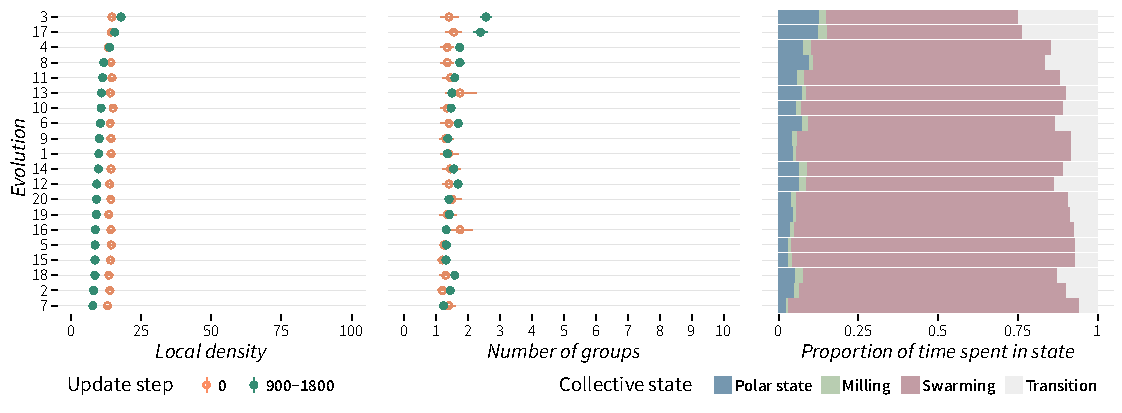
\includegraphics[width=\figurewidth]{plos/figS1}
  \infigurecaption{To verify that the living area does not overly promote grouping behaviour we performed 20 evolutionary runs with no predators present. Each evolved behaviour was evaluated by running 20 replicates of a separate simulation. For ease of comparison the graphs present the same data as in \figurename~\ref{fig3}, this time however for evolutionary runs with no predators present. In all cases there was practically no grouping. Note that local density in all but two cases decreased rather then increased. The prey agents learned to spread out over the entire living area, to stay inside the borders of the living area, and to avoid each other (prevent collisions). In all cases the local density, polarization and rotation were very low, which resulted in a scattered swarming behaviour (see \videoname~\ref{video:V1:plos}). Note that the evolved swarming behaviour is very different with respect to the behaviour that evolved in the case when predators were present (see \videoname~\ref{video:V2:plos}). In the latter case prey learned also to group and react to predator attacks.}
  \caption{Local density, number of groups and time spent in a specific collective state for control evolutionary runs.}
  \label{figC1}
\end{figure}

\begin{video}
  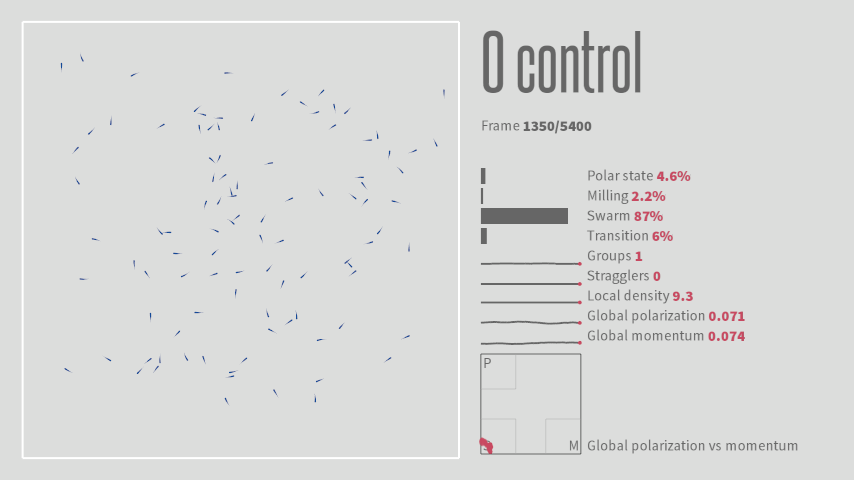
\includegraphics[width=\figurewidth]{plos/V1_1350}
  \infigurecaption{Local density, polarization and rotation are very low throughout the entire simulation run and the evolved behaviour can be classified as scattered swarming behaviour. The prey agents learned to spread out over the entire living area, to stay inside the borders of the living area, and to avoid each other (prevent collisions). Note that the evolved swarming behaviour is very different with respect to the behaviour that evolved in the case when predators were present (see \videoname~\ref{video:V2:plos}). In the latter case prey learned also to group and react to predator attacks.}
  \caption{Video sequence portraying a representative behaviour for the case of evolutionary runs with no predator present.}
  \label{video:V1:plos}
\end{video}

\clearpage % force videos V5 and V6 to appear on separate pages

\begin{video}
  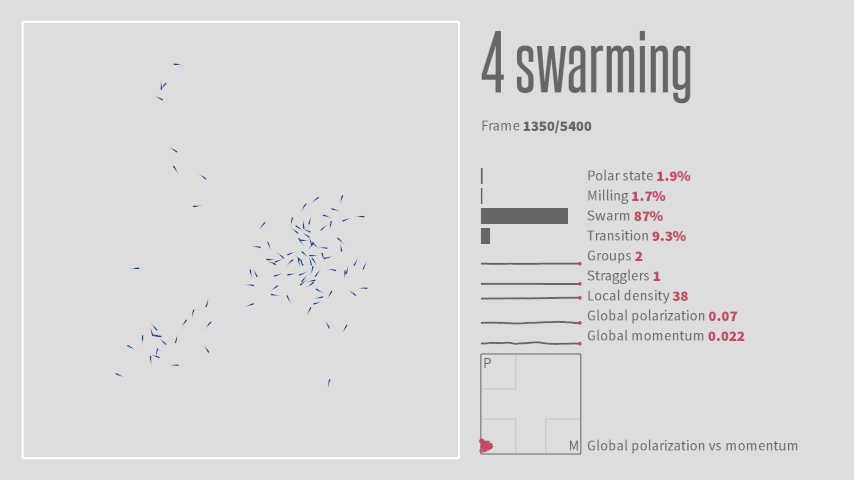
\includegraphics[width=\figurewidth]{plos/V2_1350}
  \infigurecaption{Polarization and rotation are very low throughout the entire simulation run and the evolved behaviour can be classified as swarming behaviour. Note that the local density is higher than in the case of evolutions with no predator present (see \videoname~\ref{video:V1:plos}). Prey agents learned to stay inside the borders of the living area, and to avoid each other (prevent collisions). They learned also to group (by circling each other in an unordered fashion) and react to predator attacks (see frames \numrange{3700}{3800} and \numrange{4600}{5000}). Note that soon after the disturbances induced by the predator attacks the swarming behaviour re-stabilizes.}
  \caption{Video sequence portraying a representative of the evolved swarming behaviour (evolution no.~4).}
  \label{video:V2:plos}
\end{video}

\begin{video}
  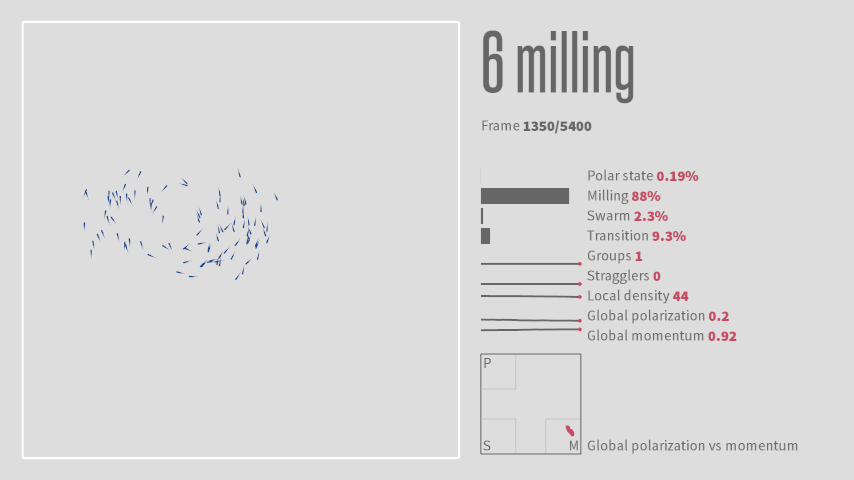
\includegraphics[width=\figurewidth]{plos/V3_1350}
  \infigurecaption{Polarization is low and rotation high throughout the entire simulation run and the evolved behaviour can be classified as milling behaviour. Note that the local density is higher than in the case when prey behaviour evolved with no predator present (see \videoname~\ref{video:V1:plos}). Prey agents learned to stay inside the borders of the living area, to avoid each other (prevent collisions) and group (by circling around an empty core in an ordered fashion), as well as react to predator attacks (see frames \numrange{1900}{2100}, \numrange{2700}{2900} and \numrange{4700}{5000}). At frame \numrange{4900}{4950} one can also observe the formation of a vacuole. Note that soon after the disturbances induced by the predator attacks the milling behaviour re-stabilizes.}
  \caption{Video sequence portraying a representative of the evolved milling behaviour (evolution no.~6).}
  \label{video:V3:plos}
\end{video}

\begin{video}
  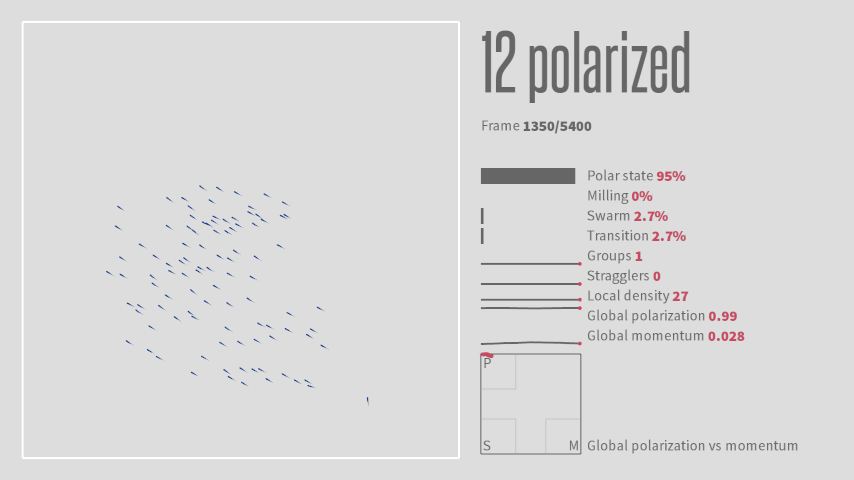
\includegraphics[width=\figurewidth]{plos/V4_1350}
  \infigurecaption{Polarization is very high and rotation low throughout the entire simulation run and the evolved behaviour can be classified as polarized behaviour. Note that the local density is higher than in the case when prey behaviour evolved with no predator present (see \videoname~\ref{video:V1:plos}). Prey agents learned to stay inside the borders of the living area, to avoid each other (prevent collisions) and group (by matching each other's heading). Prey agents learned also to react to predator attacks (see frames \numrange{1800}{2000}, \numrange{2700}{2900}, \numrange{3600}{3900} and \numrange{4500}{5100}). Note that soon after the disturbances induced by the predator attacks the polarized behaviour re-stabilizes. Note also that apart from one individual all other prey agents resort to grouping and polarized behaviour, whereas the aforementioned individual does so only occasionally, evidence that in our case the behaviours of prey agents are heterogeneous (see frames \numrange{900}{2700}). For this reason the individual, however, becomes an easy target for the predator that attacks peripheral prey (see frames \numrange{2700}{2900}).}
  \caption{Video sequence portraying a representative of the evolved polarized behaviour (evolution no.~12).}
  \label{video:V4:plos}
\end{video}

\begin{video}
  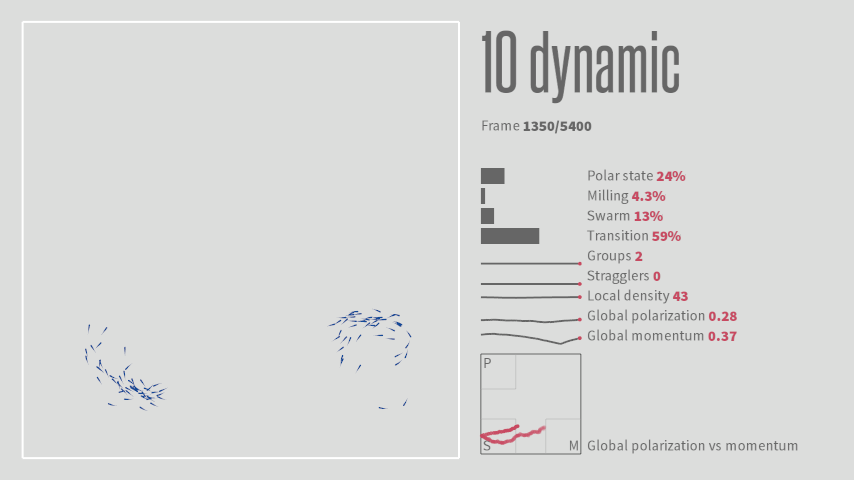
\includegraphics[width=\figurewidth]{plos/V5_1350}
  \infigurecaption{Prey agents learned to stay inside the borders of the living area, to avoid each other (prevent collisions), to react to predator attacks (see frames \numrange{1900}{2100}, \numrange{2700}{2900}, \numrange{3700}{3800} and \numrange{4700}{5100}), and to group. Note, however, that in contrast to Videos~\ref{video:V1:plos}--\ref{video:V5:plos} the prey agents in this case continuously transition between different states (polarized-milling-swarming) which results in the largest proportion of time spent in transition between states. This dynamic behaviour re-stabilizes soon after the disturbances induced by the predator attacks.}
  \caption{Video sequence portraying a representative of the evolved dynamic behaviour (evolution no.~10).}
  \label{video:V5:plos}
\end{video}

\clearpage % force videos V5 and V6 to appear on separate pages

\begin{video}
  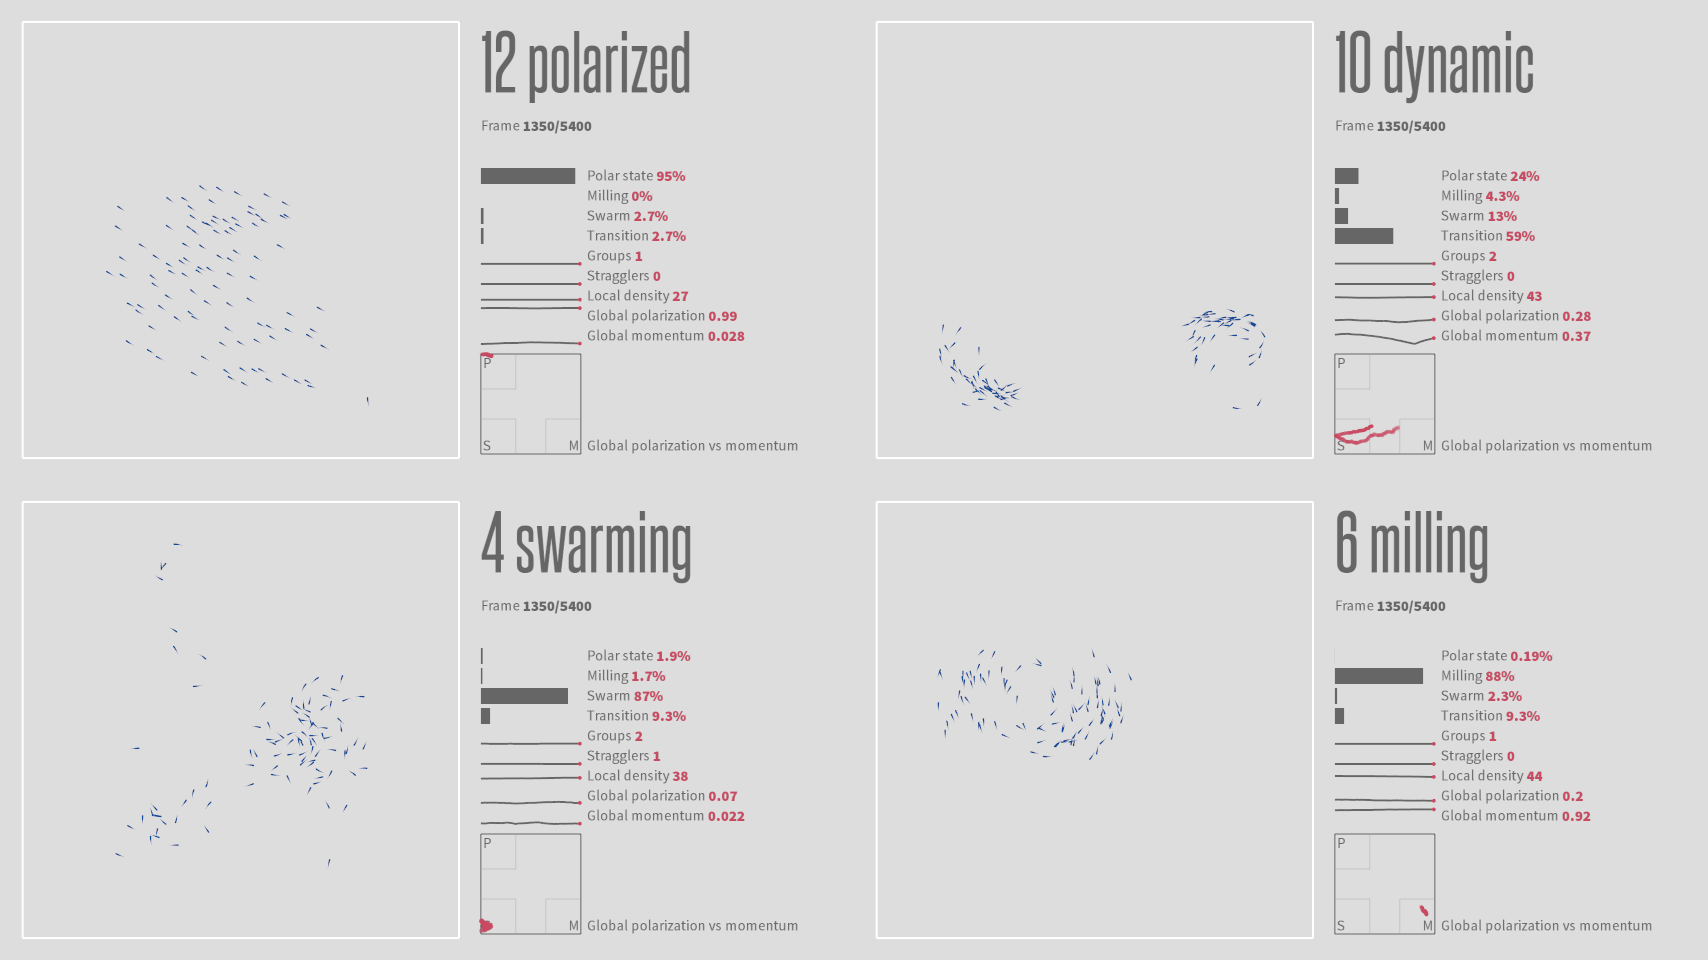
\includegraphics[width=\figurewidth]{plos/V6_1350}
  \infigurecaption{A 2\,\texttimes\,2 \textsc{hd} version where video sequences from Videos \ref{video:V2:plos}--\ref{video:V5:plos} are played in synchrony and can be observed simultaneously was constructed to ease the comparison of the representative evolved behaviours. Here available for download only. An online viewable version is available at \href{https://vimeo.com/190425371}{vimeo.com/190425371}. See captions of \videoname~\ref{video:V2:plos}--\ref{video:V5:plos} for details.}
  \caption{A \textsc{hd} video sequence where representative evolved behaviours can be observed simultaneously.}
  \label{video:V6:plos}
\end{video}

\end{subappendices}

	% !TeX root = ./thesis.tex










%==============================
\chapter[A balanced mixture of antagonistic pressures promotes\\ the evolution of parallel movement]{A balanced mixture of antagonistic pressures\\ promotes the evolution of\\ parallel movement}
\chaptermark{A balanced mixture of antagonistic pressures promotes parallel movement} % change running head for chapter
\label{chap:scirep}

\chapterAbstract[published={scirep/Demšar_etal_2016.pdf}, keywords={Collective behaviour, evolution, fuzzy logic, predator-prey interaction, dynamic parallel group}]{A common hypothesis about the origins of collective behaviour suggests that animals might live and move in groups to increase their chances of surviving predator attacks. This hypothesis is supported by several studies that use computational models to simulate natural evolution. These studies, however, either tune an ad-hoc model to ``reproduce'' collective behaviour, or concentrate on a single type of predation pressure, or infer the emergence of collective behaviour from an increase in prey density. In nature, prey are often targeted by multiple predator species simultaneously and this might have played a pivotal role in the evolution of collective behaviour. We expand on previous research by using an evolutionary rule-based system to simulate the evolution of prey behaviour when prey are subject to multiple simultaneous predation pressures. We analyse the evolved behaviour via prey density, polarization, and angular momentum. Our results suggest that a mixture of antagonistic external pressures that simultaneously steer prey towards grouping and dispersing might be required for prey individuals to evolve dynamic parallel movement.}

%-----
\section{Introduction}

Results from studies of collective behaviour are useful for scientists from many different research fields -- from biology, physics and medicine, to computer science \cite{deisboeck2009collective,lebarbajec2009organized,sumpter2006principles,vicsek1995novel,xu2014crowd}. Because humans behave similarly as groups of animals in a wide repertoire of situations, such as traffic jams and behaviour at large-scale events (\eg sport games, music concerts), collective behaviour is also interesting from the social studies perspective \cite{sumpter2006principles,xu2014crowd}.

The literature about collective behaviour contains several hypotheses about why animals, such as schools of fish, flocks of birds, swarms of insects, and herds of ungulates coalesce into groups. Some studies suggest that animal groups may increase the mating and foraging efficiency of their members \cite{krebs1994behavioural}, or that grouping could save energy because of hydrodynamic or aerodynamic benefits \cite{hemelrijk2014increased,marras2015fish,portugal2014upwash}.

Probably the most common hypotheses about the evolution of collective behaviour are related to protection from predation \cite{cresswell2011predicting,hart2005predator,krause2002living,larsson2012why,lebarbajec2009organized,nishimura2002predator,pavlov2000patterns}. The selfish herd hypothesis suggests that animals form groups in order to reduce their individual domain of danger \cite{hamilton1971geometry,kimbell2015selfish,morrell2015consequences}. The confusion effect hypothesis states that a predator attacking a group of visually similar prey might have a hard time tracking and capturing its target \cite{demsar2015simulating,kunz2006prey,nishimura2002predator,olson2013predator,olson2016evolution,zheng2005behavior}. The many eyes hypothesis suggests that as the size of the group increases the amount of time an individual has to scan the environment decreases \cite{haley2014exploring,ruxton2008application}. And the dilution of risk hypothesis suggests that the chance of a single prey being selected as the predator's target is lower in larger groups \cite{tosh2011conditions}.

Computational models are becoming a frequent tool for studying various hypotheses concerning collective behaviour \cite{lebarbajec2009organized,sumpter2006principles,vicsek2012collective}. In computational models genetic algorithms \cite{holland1992adaptation} and genetic programming \cite{koza1992genetic} are usually used to simulate artificial evolution. Artificial evolution can help us understand which selective pressures may have been the reason for collective behaviour to evolve. Wood \& Ackland \cite{wood2007evolving} used genetic algorithms to tune parameters of the model that was originally presented by Couzin\etal \cite{couzin2002collective} to suggest that predation might promote the evolution of laterally expanded visual perception. Kunz\etal \cite{kunz2006prey} evolved artificial neural networks to show that the presence of a confusable predator might be a sufficient condition for prey individuals to evolve collective behaviour. Using a comparable technique, a similar result was achieved by Olson\etal \cite{olson2013predator,olson2016evolution}, who in addition showed that predators may reduce the benefits of prey grouping by attacking peripheral targets and that grouping evolves when the predators attack prey individuals that are located nearby. Morrell\etal \cite{morrell2015consequences} showed that complex rules outperform simple ones under a range of predator attack strategies. As a contrast Demšar\etal \cite{demsar2015simulating} used genetic algorithms to evolve composite predation tactics and showed that confusion might play an important role in the evolution of these. A recent study by Biswas\etal \cite{biswas2014causes} suggests that the dilution of risk is the most prominent factor for the evolution of clumping and not the confusion effect as suggested by previous research. 

In the studies that investigated the evolution of collective behaviour under various predation tactics \cite{biswas2014causes,morrell2015consequences,olson2013predator,olson2016evolution} researchers were mostly interested in whether prey individuals start to group or not (\ie whether as a result of the artificial evolution the prey density increased or decreased). As groups of animals in nature move in many different regimes (clumping, swarming, milling, schooling, etc.) \cite{krause2002living,suzuki1973movement} and different predation pressures are countered by different responses of prey groups, we can hypothesise that the type of predation tactic has an influence on the type of collective behaviour that evolves.

In this study we focus on how predation from various types of predators influences the evolution of collective behaviour in prey individuals. We let prey individuals evolve their behaviour while experiencing predation from a) predators for which grouping might be a natural response and b) predators for which dispersing might be a natural response. According to previous research there are several predation tactics that pressure prey individuals to evolve grouping behaviour \cite{biswas2014causes,kunz2006prey,olson2013predator,olson2016evolution}. Two of these are a) attack prey individuals located at the periphery of the prey group (P, periphery) and b) attack the nearest prey individual (N, nearest). Predation tactics that pressure prey towards dispersing (against grouping behaviour), are a) attack the most central prey individual in a prey group (C, centre) and b) high density area attacks (H, density) \cite{olson2013predator}. 

Predators that attack the nearest, the most peripheral or the most central prey individual usually detect, pursue, attack and capture a single prey individual. For example, black seabass, \emph{Centropristis striata}, in attacks on schools of Atlantic silversides, \emph{Menidia menidia}, focus on stragglers when these are available, otherwise they most often target central prey \cite{parrish1989reexamining}. Predators that focus on nearest prey individuals are typically sit-and-wait, ambush or surprise-attack predators (\eg largemouth bass, \emph{Micropterus salmoides} \cite{savino1982predatorprey} or peregrine falcons, \emph{Falco peregrinus}\cite{zoratto2010aerial}) who try to minimize energy costs required for prey capture. However, rather than relying on a single predation tactic predators usually adapt their tactic with respect to the prey species. For example, in attacks on either free-swimming whirligig beetles, \emph{Dineutes discolor}, or a constrained group of tadpoles, \emph{Bufo bufo}, largemouth bass, \emph{Micropterous salmoides}, like goldfish, \emph{Carassius auratus}, preferentially attack prey on the periphery \cite{romey2008predators}. Recent research by Ioannou\etal \cite{ioannou2012predatory} showed that bluegill sunfish, \emph{Lepomis macrochirus}, when hunting virtual prey disproportionately more often attack prey relatively far from the group centre, but only in the case when prey individuals are moving with relatively low tortuosity. In attacks on groups, on the other hand, prey in groups with a coordinated direction of motion (\ie, with high polarization) were at less risk than their counterparts in unpolarized swarms.

Density attacking predators are usually larger than a single prey individual and do not necessarily detect, pursue, attack and capture a single prey individual, but can attack and capture several prey individuals in a single predation event (\eg whales). Minke whales, \emph{Balaenoptera acutorostrata}, lunge feed on small schooling fish \cite{hoelzel1989foraging}. Killer whales, \emph{Orcinus orca}, are known to use cooperative hunting \cite{domenici2000killer,nottestad1999herring}. Basking sharks, \emph{Cetorhinus maximus}, on the other hand, are filter-feeders and feed while cruising at a relatively low and constant speed \cite{sims2000filterfeeding}. In these cases, while the prey may be able to accelerate and manoeuvre at a higher rate than the predator, the difference in size is such that, once the prey is aimed at, its speed is too low to avoid the predator's large gape \cite{domenici2001scaling}. In nature, prey living in groups are often targeted by such predators \cite{domenici2001scaling,goldbogen2011mechanics,nottestad1999herring,nottestad2002whales}, and scenarios where prey are subject to multiple predation tactics simultaneously (\eg attack single peripheral prey individuals, and density attacks) are not uncommon (\eg multi-species feedings)\cite{haynes2013molecular,mori2006first,thiebault2015howto}. Exposure to such conflicting, antagonistic predation pressures might have played a pivotal role in the evolution of collective behaviour. For this reason we investigated the type of evolved behaviour when varying exposure to multiple (conforming and antagonistic) simultaneous predation pressures.

\section{Results}

The influence of predation pressures on the evolution of prey behaviour was studied by varying the number of predators using different specific predation tactics. The total number of predators used to obtain results reported in this study was eight, but no significant difference was observed while performing preliminary tests with larger or smaller numbers of predators.

\begin{figure}
	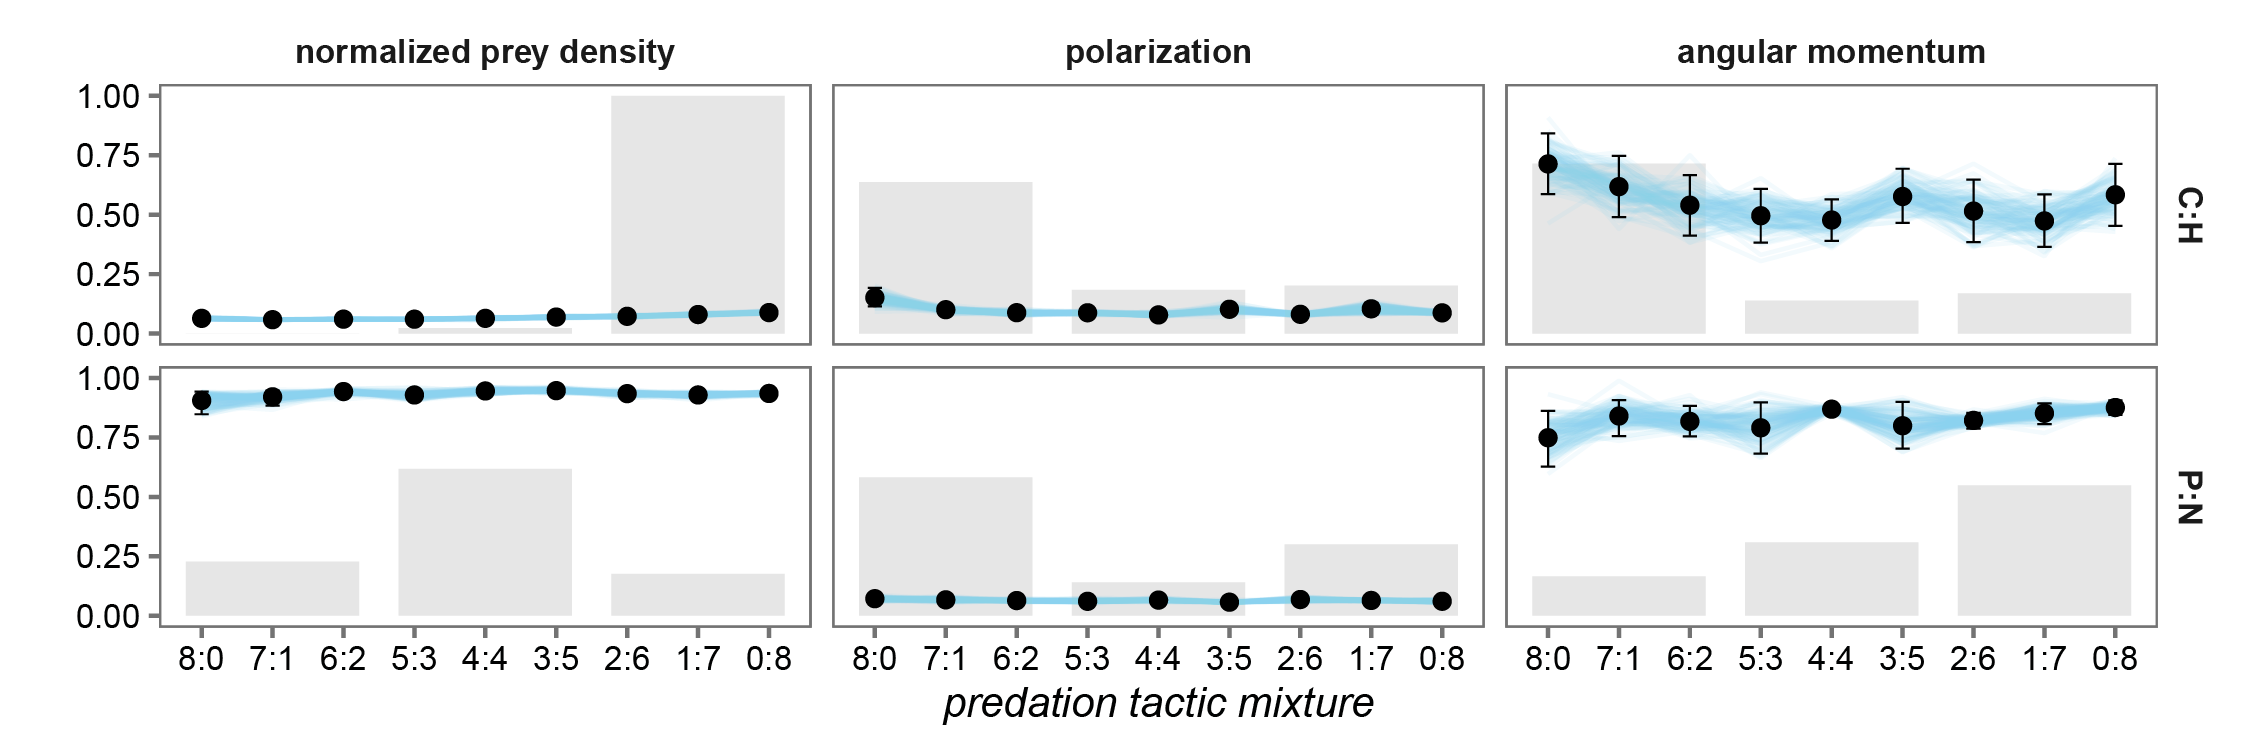
\includegraphics[width=\figurewidth]{scirep/dpm_conforming}
	\infigurecaption{P -- attack prey individuals located at the periphery of prey groups, N -- attack the nearest prey individual, C -- attack the most central prey individual in a prey group, and H -- high density area attacks. The predation pressure mixture ratio \emph{a}:\emph{b} denotes the number of predators using a specific predation tactic, \eg in the case of C:H, 0:8 (top row, right side of the plot) all predators (eight) use high density area attacks. Points and whiskers represent the estimated posterior means and 95\% posterior confidence intervals. Individual draws from the posterior distributions are connected with lines to visualize posterior uncertainty and aid in the interpretation of how the means vary across the predation pressure mixtures. To summarize the results, the predation mixtures were grouped into groups of three: predation pressure predominantly from centre (C:H) or periphery (P:N) attacking predators (8:0, 1:7, 2:6), balanced pressure (5:3, 4:4, 3:5), and predation pressure predominantly from high density area (C:H) or nearest prey individual (P:N) attacking predators (6:2, 7:1, 0:8). The shaded bars show, for each group, the probability that that group has the highest mean. These probabilities were estimated with draws from the posterior distributions in which each group member had an equal probability of being selected. That is, each predation mixture was weighted equally.}
	\caption{Normalized prey density, polarization, and angular momentum for conforming predation pressure mixtures.}	\label{figure:conforming}
\end{figure}

According to previous studies\cite{biswas2014causes,kunz2006prey,olson2013predator,olson2016evolution} predation pressure from predators that attack the most central prey individual in a prey group (C) or use high density area attacks (H) should promote the evolution of the tendency to disperse in prey individuals. On the other hand, predation pressure from predators that attack prey individuals located at the periphery of the prey groups (P) or the nearest prey individual (N) should lead to the evolution of the tendency to group. As from the point of view of the expected outcome in both cases the two predation tactics agree, regardless of the number of predators using a specific tactic (dispersion for combination C:H, grouping for P:N), we call such predation pressures conforming. Our results (\figurename~\ref{figure:conforming}) support previous studies. With conforming pressures towards dispersing by centre and density attacking predators the mean normalized prey density consistently stayed below \num{0.125}, regardless of the number of predators using a specific tactic. On the other hand, with conforming pressures towards grouping by periphery and nearest prey individual attacking predators the mean normalized prey density remained above \num{0.75}, regardless of the number of predators using a specific tactic.

Couzin\etal \cite{couzin2002collective} introduced the measures of polarization and angular momentum. They express the degree of consensus in a common heading of the group (polarization), and the degree of rotation of the group about the group's centre (angular momentum). By means of these two measures Couzin\etal \cite{couzin2002collective} defined four collective dynamical behaviours: swarm (low polarization and low angular momentum), torus or milling (low polarization and high angular momentum), dynamic parallel group (high polarization and low angular momentum), and highly parallel group (very high polarization and low angular momentum) \cite{couzin2002collective}. 

Conforming predation pressures (combinations C:H and P:N in \figurename~\ref{figure:conforming}) resulted in behaviours with medium to high angular momentum and low polarization. While polarization was low for all pressure mixtures, its mean was highest when predation pressure came predominantly from centre or periphery attacking predators. Predation pressures for which the response was grouping led to consistently high angular momentum with low variability. Here attacks directed predominantly on the nearest prey individual gave rise to the highest mean angular momentum. The high angular momentum combined with the consistently low polarization suggests the evolution of milling behaviours. Pressure towards dispersing, on the other hand, resulted in substantially lower angular momentum with a higher variability. Here, domination by centre attacking predators induced the highest mean angular momentum. As polarization was low the medium to high angular momentum with high variability suggests the evolution of either swarming or milling behaviours. Note here that even in cases where polarization was the highest it was not high enough to suggest the observed behaviour could be classified as polarized.

\begin{figure}
	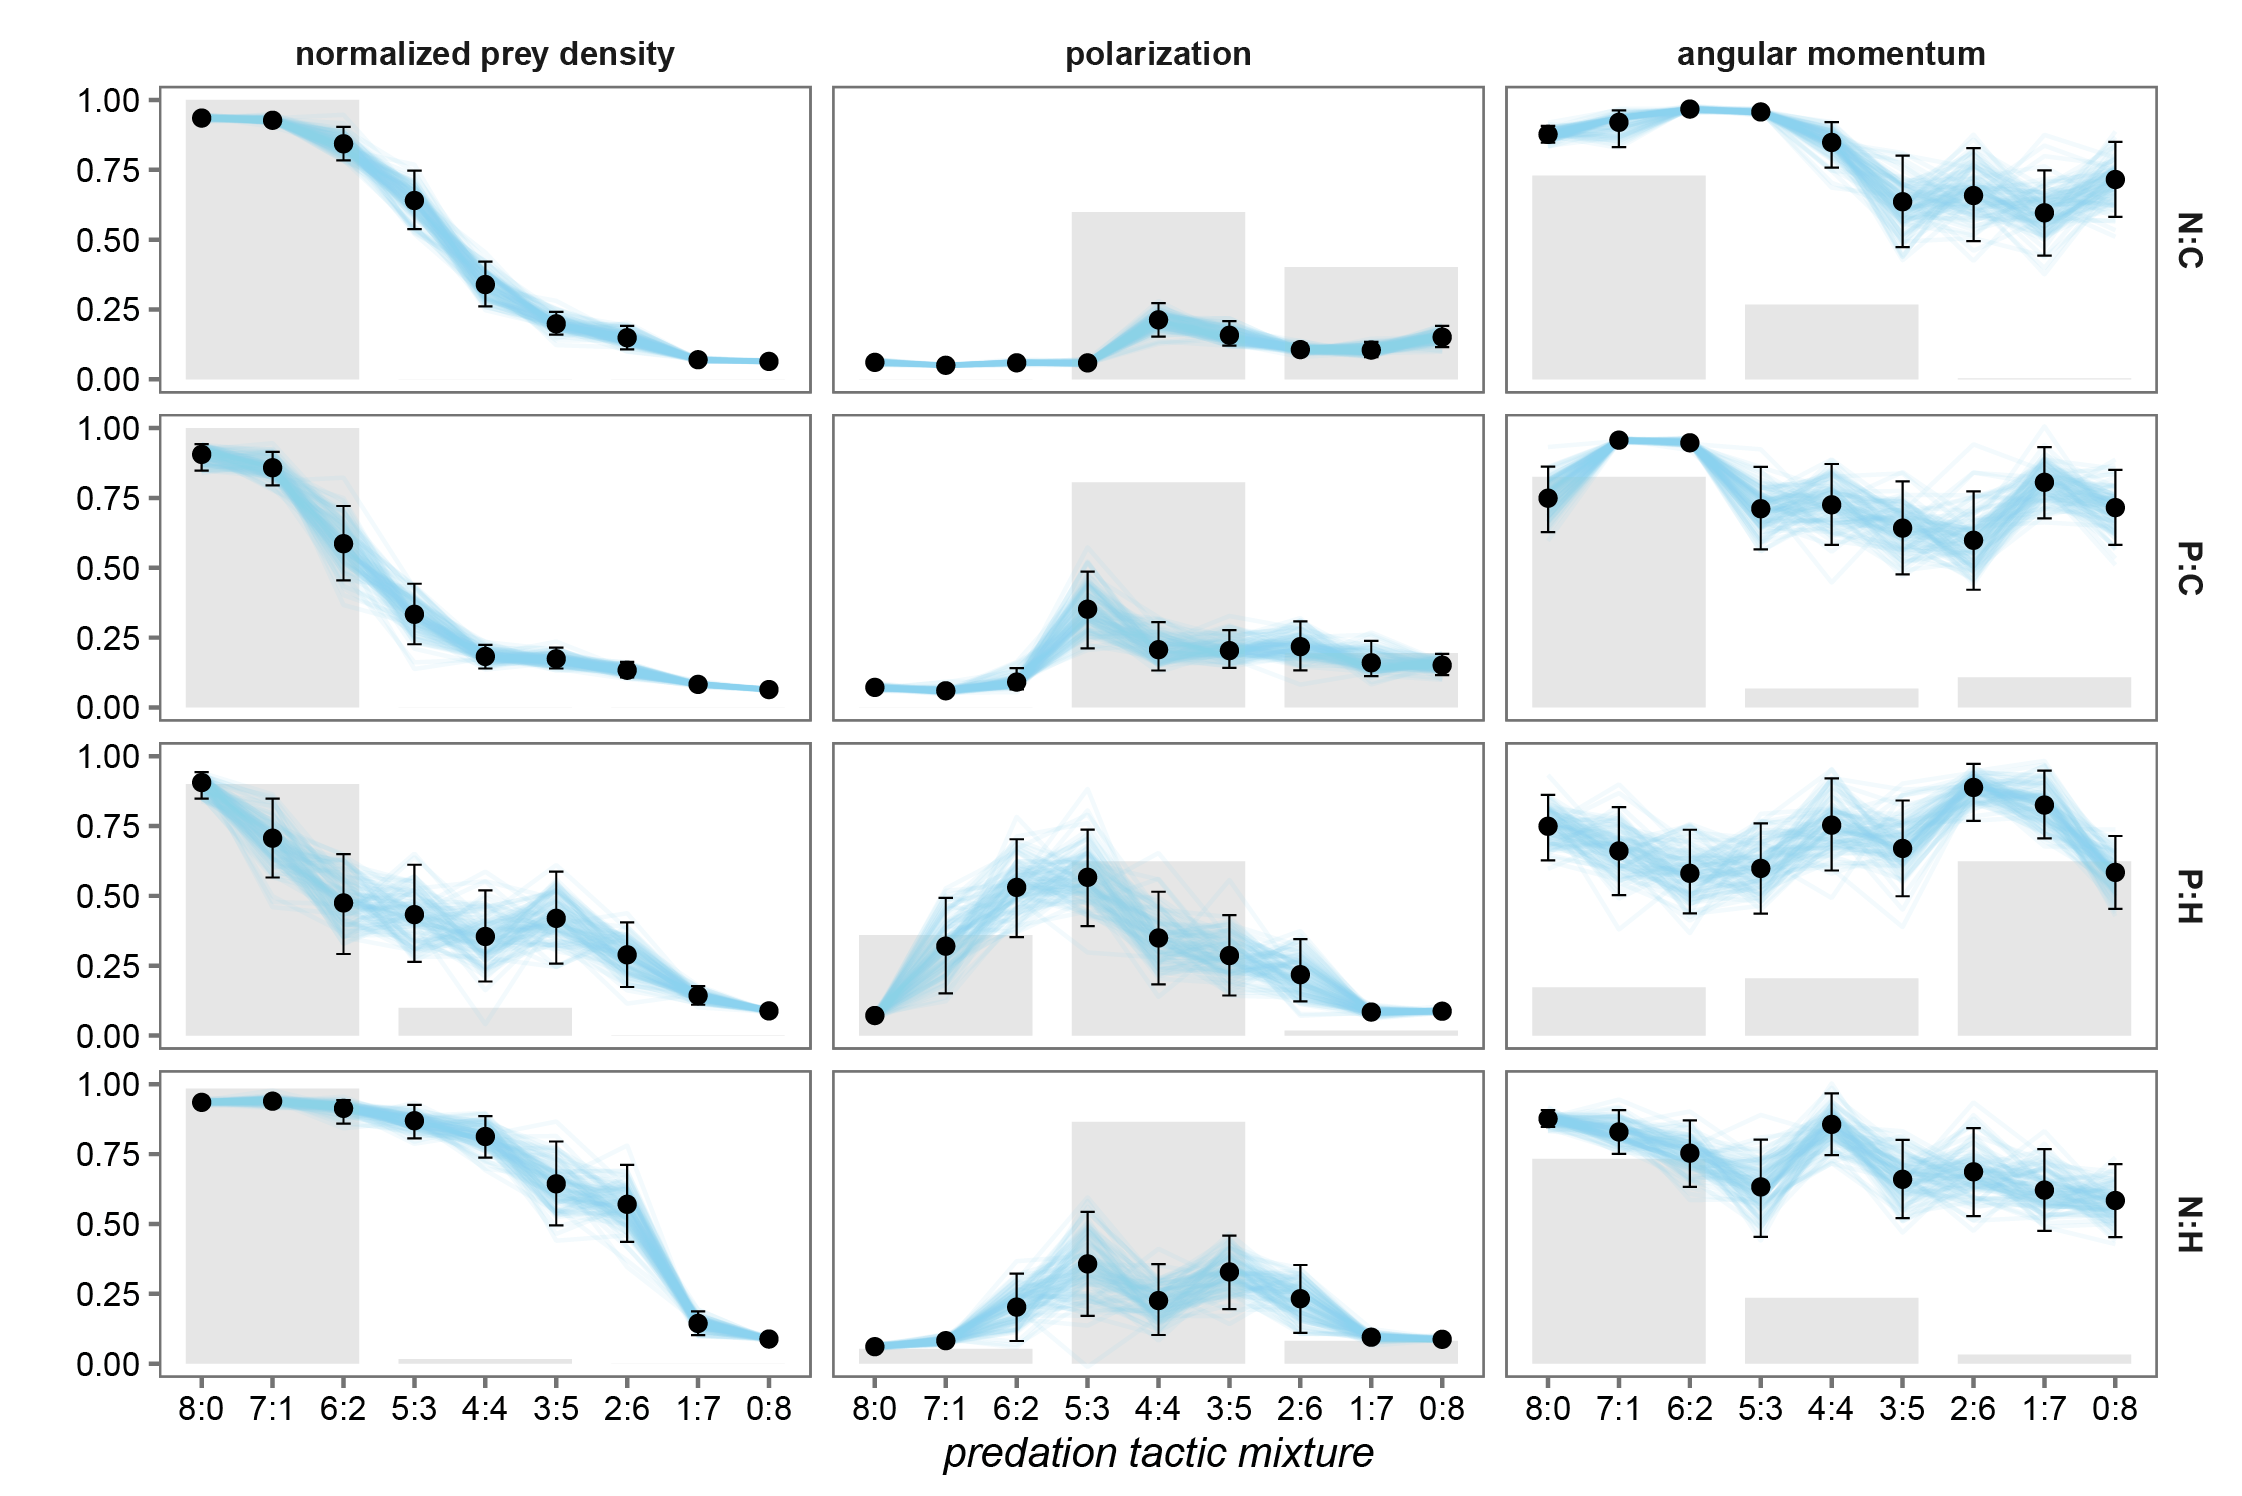
\includegraphics[width=\figurewidth]{scirep/dpm_antagonistic}
	\infigurecaption{P -- attack prey individuals located at the periphery of prey groups, N -- attack the nearest prey individual, C -- attack the most central prey individual in a prey group, and H -- high density area attacks. The predation pressure mixture ratio \emph{a}:\emph{b} denotes the proportion of predators using a specific predation tactic, \eg in the case of N:C, 0:8 (top row, right side of the plot) all predators (eight) attack the most central prey individual in a prey group. Points and whiskers represent the estimated posterior means and 95\% posterior confidence intervals. Individual draws from the posterior distributions are connected with lines to visualize posterior uncertainty and aid in the interpretation of how the means vary across the predation pressure mixtures. To summarize the results, the predation mixtures were grouped into groups of three: low degree of antagonism in predation pressures with predominant pressure from predators that force prey into grouping (8:0, 1:7, 2:6), high degree of antagonism in predation pressures (5:3, 4:4, 3:5), and low degree of antagonism in predation pressures with predominant pressure from predators that force prey into dispersion (6:2, 7:1, 0:8). The shaded bars show, for each group, the probability that that group has the highest mean. These probabilities were estimated with draws from the posterior distributions in which each group member had an equal probability of being selected. That is, each predation mixture was weighted equally.}
	\caption{Normalized prey density, polarization, and angular momentum for antagonistic predation pressure mixtures.}
	\label{figure:antagonistic}
\end{figure}

In the case of antagonistic predation pressures (combinations N:C, N:H, P:C and P:H, see \figurename~\ref{figure:antagonistic}) the highest mean normalized prey density emerged when predation pressure came predominantly from the nearest or the most peripheral prey individual attacking predators (predators that in a conforming setting pressure prey into grouping; mixtures 8:0, 7:1, 6:2). On the other hand, domination by predators for which the expected outcome is dispersing (mixtures 2:6, 1:7, 0:8) led to the lowest mean normalized prey density. Domination by either pressure to group or pressure to disperse can be interpreted as a low degree of antagonism in predation pressures. A high degree of antagonism, where neither the pressure to disperse nor the pressure to group dominates (mixtures 5:3, 4:4, 3:5), led to the evolution of low to high mean normalized prey density. The lowest in the case of periphery and centre attacking predators (P:C) and highest in the case of nearest prey individual and high density area directed attacks (P:H).

Evolution under antagonistic predation pressures resulted in medium to high angular momentum and low to medium polarization. Compared to the case of conforming predation pressures, there was a considerably higher variability in the values of angular momentum and polarization, suggesting a wider range of evolved behaviours. In all but the P:H case, predation pressure predominantly from predators that result in prey individuals that favour grouping gave rise to the highest angular momentum. In the P:H case, on the other hand, it was highest when the pressure to disperse dominated. Note that angular momentum was never the highest when antagonism in predation pressures was high (predation pressure mixtures 5:3, 4:4, 3:5). High antagonism, however, always generated the highest mean polarization.

Observing all three parameters in unison (see Supplementary information, \figurename~\ref{figure:antagonistic:SM}) suggests that increasing the pressure towards dispersing from centre or high density area attacking predators leads to a general decrease in normalized prey density, angular momentum and polarization (top and right portion of the figure). An increase in pressure towards grouping from predators that attack the nearest or the most peripheral prey individual, on the other hand, causes an increase in density and a favouring of higher momentum with low polarization (bottom and left portion of the figure). Higher values of polarization with low momentum and medium density emerge when the mixture in pressures towards and against grouping (towards dispersing) is somewhat balanced. This suggests a possible emergence of polarized behaviour. 

\begin{figure}
	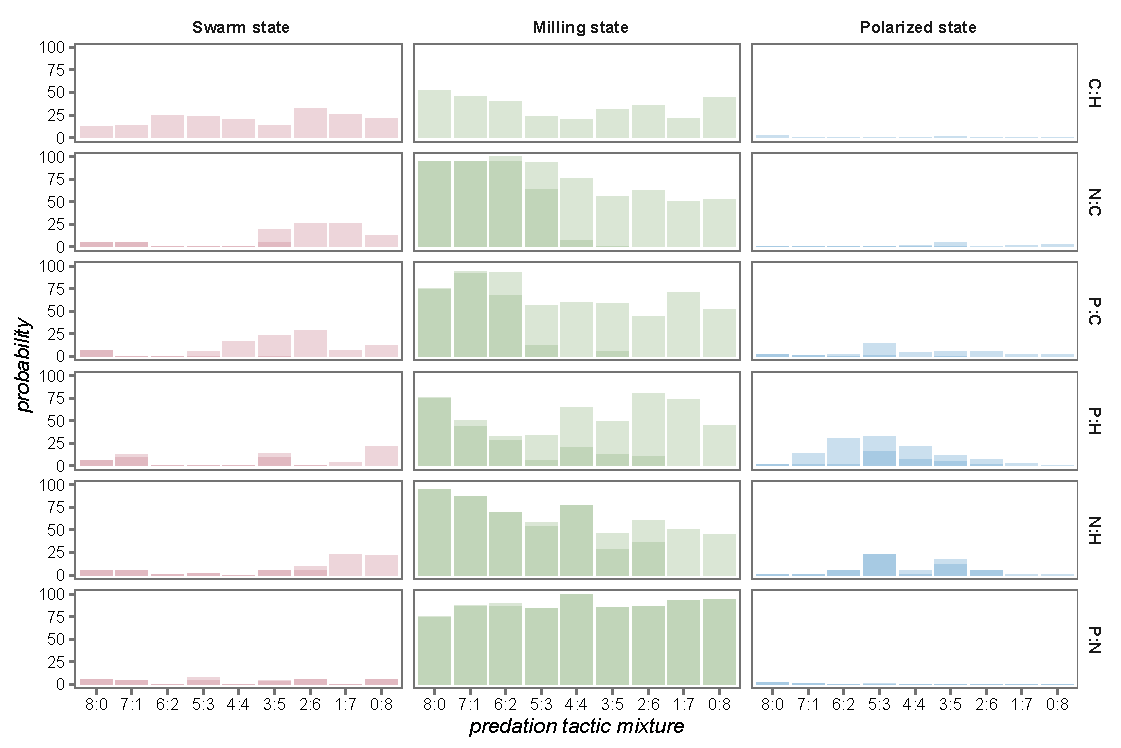
\includegraphics[width=\linewidth]{scirep/class_t__35_1800_final}
	\infigurecaption{P -- attack prey individuals located at the periphery of prey groups, N -- attack the nearest prey individual, C -- attack the most central prey individual in a prey group, and H -- high density area attacks. The shading denotes cases with low (light shading) and high normalized prey density (dark shading). The predation pressure mixture ratio \emph{a}:\emph{b} denotes the proportion of predators using a specific predation tactic, \eg in the case of C:H, 8:0 (top row, left side of the plot) all predators (eight) attack the most central prey individual in a prey group.}
	\caption{The probability of observing a specific collective state at the end of the simulation run for all predation pressure mixtures.}
	\label{figure:classification}
\end{figure}

Note that polarization and angular momentum reported in \figurename s~\ref{figure:conforming}, \ref{figure:antagonistic} and \ref{figure:antagonistic:SM}, although indicative of the resulting behaviour, cannot be used for such a classification directly, because they were computed as weighted sums of polarization and angular momentum of individual groups and averaged over a number of frames (see Methods). Therefore, to further analyse the influence of predation pressures on the evolution of prey behaviour, we categorized the behaviour of individual groups with respect to their polarization and angular momentum in the last frame of of every simulation run. Here we followed Tunstrøm\etal \cite{tunstrom2013collective}, who used polarization and angular momentum and a simple threshold to categorize the behaviour of groups of golden shiners, \emph{Notemigonus crysoleucas}, into one of three collective states; swarm, milling, and polarized state. Based on that we computed the probability of observing a particular collective state (see Methods). This analysis provides further insight into what kind of behaviour evolves under a particular predation pressure mixture ratio. \figurename~\ref{figure:classification} confirms what was suggested by data presented in \figurename s~\ref{figure:conforming}, \ref{figure:antagonistic} and \ref{figure:antagonistic:SM}: the probability of observing the swarm state is present mainly in cases when prey individuals evolved while under predation pressure from centre or high density area attacking predators. The probability of observing a swarm state is the highest when prey individuals evolved under conforming pressures towards dispersing by centre and density attacking predators. Overall, the probability of observing a milling state dominates, and is high in most cases, except when: a) prey individuals evolved under conforming pressures towards dispersing by centre and density attacking predators, and b) prey individuals evolved under certain antagonistic pressures. On the other hand, evolution under antagonistic pressures produced the highest probability of observing a polarized state. This suggests that a mixture of antagonistic pressures that simultaneously steer prey towards grouping and dispersing might be required for prey individuals to evolve parallel movement.

Visual inspections of the evolved behaviours confirmed that the domination of predation pressures towards dispersing led prey to evolve behaviours where they in general tend to disperse. This tendency to disperse at times leads to the wall-following of the living area border and thus while keeping a low density causes a relatively high angular momentum (see Supplementary information, \videoname~\ref{video:V1}). As this is classified as milling, the probability of observing the milling state dominates in \figurename~\ref{figure:classification}. The solution being classified as milling is probably irrelevant for biological organisms as it is determined by the artificial ecology used for this computational study (\ie crossing the living area border would sooner or later be lethal for the prey individual). Nevertheless, in an experiment with zebrafish, \emph{Danio rerio}, the distribution of the positions detected in the tank showed that the fish avoid the centre of the tank and the higher probability of presence is along the walls \cite{collignon2016stochastic}, which might be indicative of a similar form of wall-following. On other occasions with low density the evolved behaviour resembled collective motion typically identified as swarming, associated with low angular momentum, and low polarization (see Supplementary information, \videoname~\ref{video:V2}). Predation pressure predominantly from predators that push prey into grouping led prey individuals to evolve behaviours that usually resulted in high density, high angular momentum and low polarization, values typically associated with milling (see Supplementary information, \videoname~\ref{video:V3}). On few occasions the evolved behaviour resulted in high density, low angular momentum and low polarization, indicative of high density swarming (see Supplementary information, \videoname~\ref{video:V4}). As suggested by data presented in \figurename s~\ref{figure:antagonistic} and \ref{figure:classification} behaviours with higher values of polarization emerged mostly when there was a high degree of antagonism in predation pressures (\ie when there was a balanced mixture of pressure towards and against grouping). Here prey individuals often evolved behaviours that resulted in parameter values typical for dynamic and highly parallel motion; medium to high normalized density, low to medium angular momentum and medium to high polarization (see Supplementary information, \videoname s~\ref{video:V5}--\ref{video:V7}).

%-----
\section{Discussion}

Previous research that used evolutionary computational models to study the evolution of collective behaviour\cite{biswas2014causes,kunz2006prey,morrell2015consequences,olson2013predator,olson2016evolution} suggests that prey grouping might have evolved as a defensive mechanism against predation. Most of the existing studies were principally interested in whether prey evolve a) grouping behaviour (defined as an increase in prey density) or b) dispersing behaviour (defined as a decrease in prey density). Our study corroborates previous findings in that prey density is high when prey individuals evolve while under predation pressure from predators for which grouping might be a natural response (attack peripheral prey individuals, or attack the nearest prey individual), and low when prey individuals evolve while under predation pressure from predators for which dispersing might be a natural response (attack the most central prey individual, or attack high density areas).

Groups of animals in nature, however, move in many different fashions (clumping, swarming, milling, schooling, etc.) \cite{krause2002living,suzuki1973movement} and different predation pressures are countered by different responses. As these responses are experience dependant\cite{elmasri2012response,hellstrom2016balancing}, we can hypothesise that if collective behaviour evolved as an anti-predator response it might as well have been shaped by the predation pressures the prey faced. In this study we therefore expanded on previous research by focusing on how predation from various types of predators might influence the evolution of collective behaviour in prey individuals. More specifically we investigated the influence of antagonism between predation pressures towards and against grouping (towards dispersing) on the type of evolved collective behaviour (evaluated via prey density, polarization and angular momentum \cite{couzin2002collective}). Our results suggest that when prey individuals evolve while under conforming predation pressures (either towards grouping or towards dispersing) the resulting behaviour has low polarization and medium to high angular momentum. When prey individuals evolve while subject to antagonistic predation pressures (towards grouping and towards dispersing, simultaneously) density and angular momentum increase with the number of predators forcing prey into grouping and decrease with the number of predators that force prey individuals into dispersing. Polarization, on the other hand, is highest when antagonism in predation pressures is high.

Our results therefore suggest that antagonism might have played an important role in the evolution of collective behaviour; that antagonism from predation pressures, environmental or internal factors could have been responsible for the evolution of a multitude of different behaviours. They could also indicate that in nature the evolution of highly polarized movement might be a result of the co-evolution of prey evasion and composite predator attack tactics \cite{demsar2015simulating}. Another possibility is that not only variation in swimming performance \cite{oufiero2016evolution}, but also the amount of variation in group behaviours might be linked to environmental factors. This supports the hypothesis that ecological constraints may shape the process used to regulate activity in many biological species \cite{gordon2014ecology}. Indeed, evolution of group responses to predation in nature is not universal, and different species might evolve very different responses to predation. This is not restricted to fish schools, as it is evident also in avian group behaviour, where the magnitude in variation of behaviours has always been a major puzzle. Why do so few bird species that fly together display organized behaviour, and why do even closely related species display major differences in flocking behaviour \cite{lebarbajec2009organized}. For example, pigeons are more closely related to swifts than they are to starlings \cite{jarvis2014wholegenome}, but they flock much more like starlings. Similarly, geese are more closely related to chickens than they are to cormorants \cite{jarvis2014wholegenome}, but they fly like cormorants.\footnote{Heppner FH, \emph{personal communication}, February, 2016} In view of our results one possible explanation for these observations might be that organized flight has evolved independently, and several times, and the differences in behaviour might have emerged because, although closely related, individual species were subject to different pressures.

In marine ecology Rieucau\etal's recent studies suggest that collective anti-predator responses in herring increase with the density of the school \cite{rieucau2014School}, and the number of sensory cues \cite{rieucau2014experimental,rieucau2015herring}. Our results suggest that the increase might be accentuated by the conflict in sensory cues. This corroborates recent results by Lemasson\etal \cite{lemasson2016sensory}, who suggest that the benefits of coordinated motion are context dependent, \ie they can potentially reduce the time prey individuals spend in dangerous areas and help them to avoid becoming isolated, yet such movement patterns can also alleviate predator confusion during a directed attack. It is important to note that exposure to predators affects prey both directly and indirectly and that plasticity in response to risk might relate to an individual's willingness to take risks \cite{abbeylee2016behavioral}. As our model is heterogeneous in the behaviour of prey individuals, our findings seem to suggest that this individuality in susceptibility to predation risk, might inevitably also lead to changes in the behaviour of the group.

In summary, while the dilution of risk might be sufficient for prey individuals to evolve grouping \cite{biswas2014causes}, and predator confusion might lead prey individuals to evolve swarming \cite{kunz2006prey,olson2013predator,olson2016evolution}, our results suggest that exposure to antagonistic predation pressures might be a necessary requirement for prey individuals to evolve parallel movement. This could indicate that the direction of evolution (grouping or dispersing) is not A versus B, but a labile result -- whether grouping or dispersing evolves depends on a) the nature of the group, and b) the pressures that the group finds itself facing.

%-----
\section{Methods}

Our individual based model consists of two types of artificial animals -- predators and prey. They coexist in a two dimensional environment confined by a circular living area, with their positions and headings at time instant $t$ given by $\vec{r}^{(i)}_t$, $\phi^{(i)}_t$. Following previous research \cite{dellorco2014simulation,demsar2014simulated,lebarbajec2005simulating,lucic2002transportation,tron2004mathematical}, the behaviour of every artificial animal in our model is governed by fuzzy logic \cite{zadeh1965fuzzy} via a fuzzy-rule-based system \cite{mamdani1974application}. A fuzzy-rule-based system enables the use of linguistic if-then rules to describe the behaviour of the artificial animals. It is specified via a fuzzy knowledge base, which consists of a fuzzy data base and a fuzzy rule base. The data base lists all input and output variables, as well as the linguistic terms (\eg near, far, etc.) that can appear in if-then rules. In addition it includes information necessary for fuzzy reasoning, \ie the method for transforming crisp data into fuzzy sets (fuzzification), the interpretation of logical connectives necessary for fuzzy reasoning, and the method for converting the fuzzy result into a real action (defuzzification). The fuzzy rule base on the other hand comprises the list of if-then rules that are assumed to be joined by the connective ``also,'' so multiple rules can fire simultaneously. When used in combination with artificial evolution a fuzzy-rule-based system is called a genetic fuzzy system \cite{cordon2004ten,fernandez2015revisiting,herrera2008genetic}. 

The fuzzy knowledge base of the predators was set following previous research \cite{demsar2014simulated} (see Supplementary information for details). In the case of prey individuals we, for reasons of simplicity, locked the fuzzy data base and evolved only the fuzzy rule base (see Supplementary information for details), but given that fuzzy-rule-based systems are deemed universal approximators \cite{castro1995fuzzy} this still provides the opportunity to potentially discover a wide repertoire of behaviours. 

At every update step the fuzzy-rule-based systems (\ie the pre-set fuzzy knowledge base in the case of predators, and the evolving fuzzy knowledge bases in the case of prey individuals) were used to compute the new heading (see \figurename~\ref{figure:FS}) and position of every artificial animal as:
%
\begin{figure}
  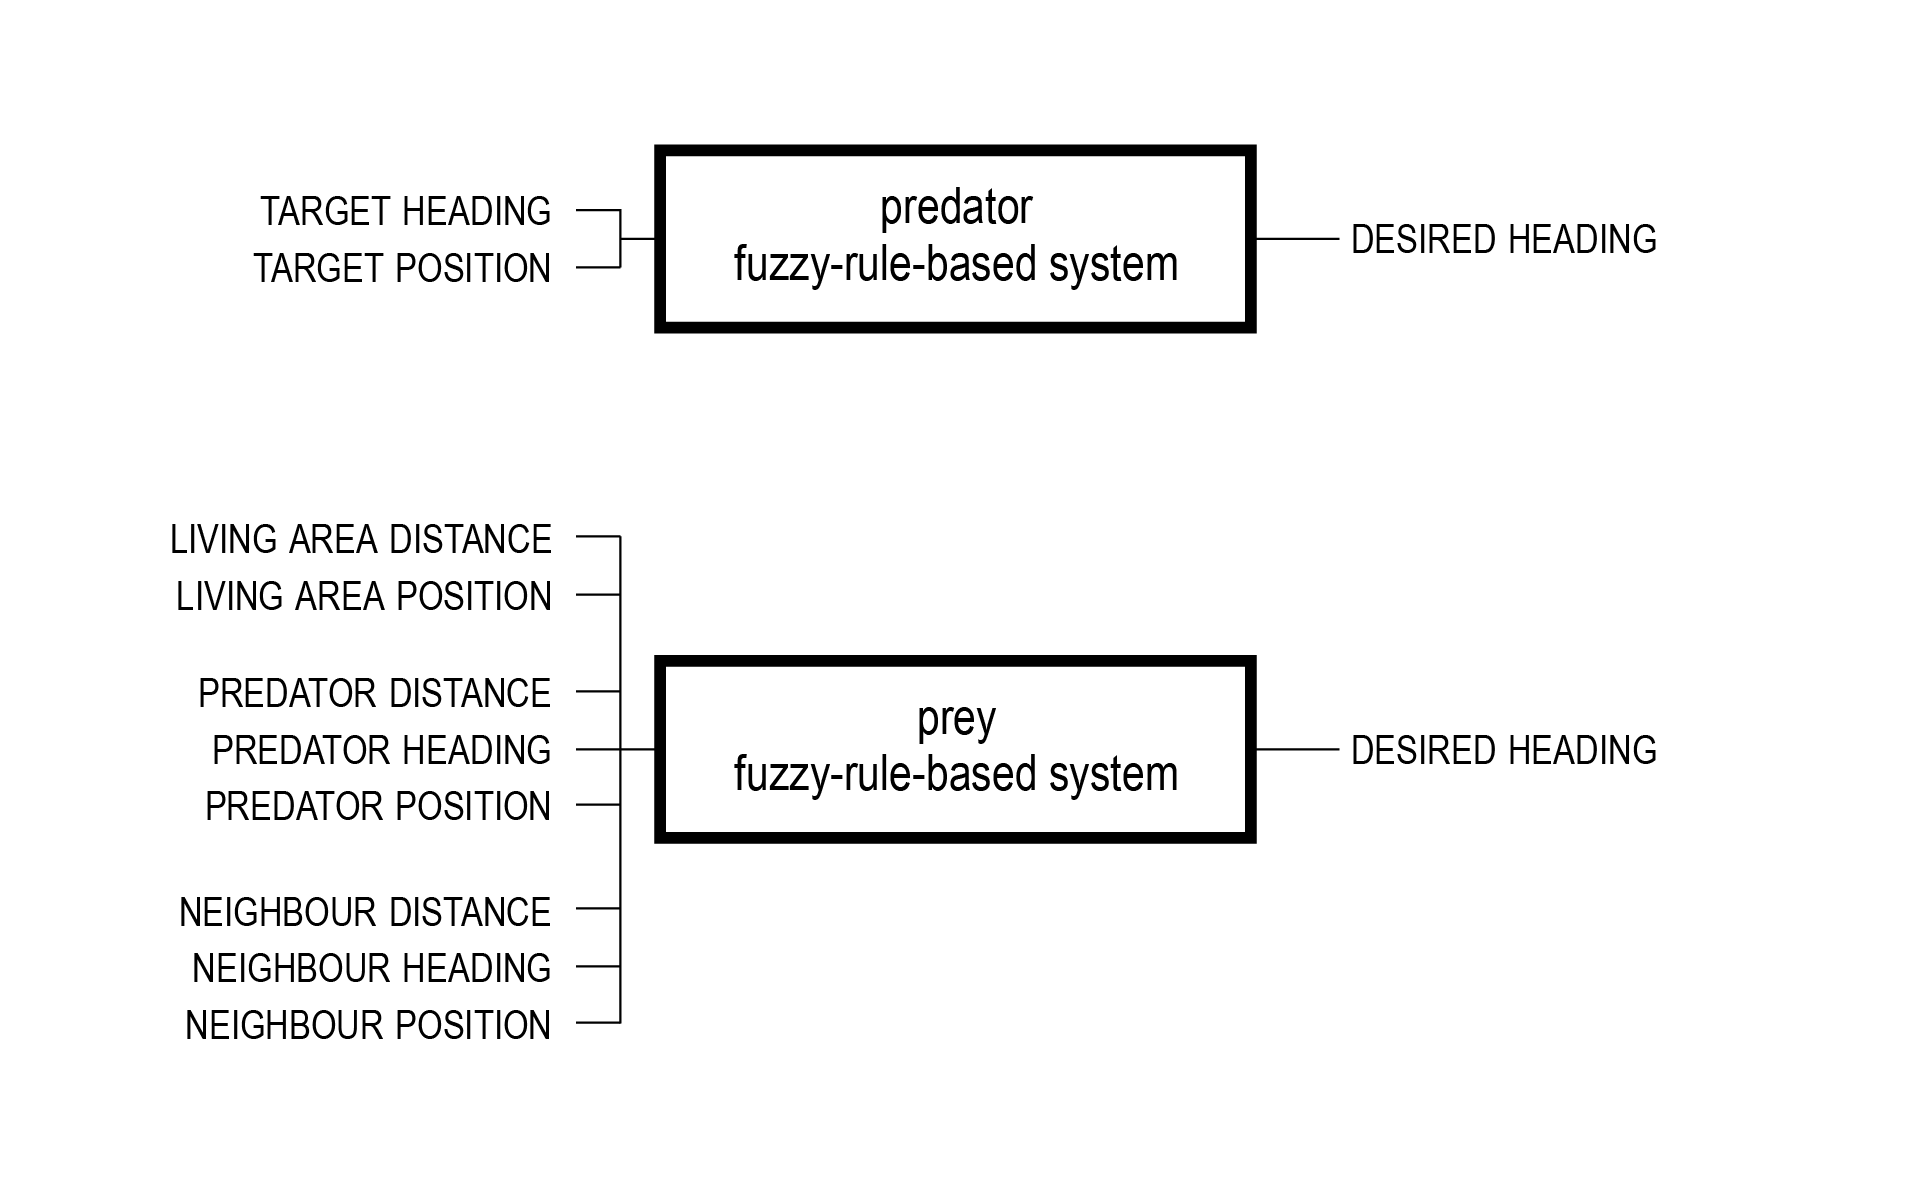
\includegraphics[width=.75\linewidth]{scirep/FS}
  \caption{A schematic showing the predator and prey fuzzy-rule-based system's input and output variables.}
  \label{figure:FS}
\end{figure}
%
\begin{equation}
%\omega^{(i)}_{t+\tau}= \min(\phi^{(i)}_t - \phi^{(i)}_\textnormal{FS},\ \omega^{(i)}_\textnormal{max}),
\omega^{(i)}_{t+\tau}= \min(\phi^{(i)}_\textnormal{FS},\ \omega^{(i)}_\textnormal{max}),
\end{equation}
%
\begin{equation}
\phi^{(i)}_{t+\tau}=\phi^{(i)}_t + \tau\omega^{(i)}_{t+\tau},
\end{equation}
%
\begin{equation}
\vec{v}^{(i)}_t=v^{(i)}\begin{bmatrix}\cos\phi^{(i)}_t \\ \sin\phi^{(i)}_t\end{bmatrix},
\end{equation}
%
\begin{equation}
\vec{r}^{(i)}_{t+\tau}= \vec{r}^{(i)}_t + \tau\vec{v}^{(i)}_{t+\tau},
\end{equation}
%
where $\phi^{(i)}_\textnormal{FS}$ is the desired heading in the local coordinate frame of individual $i$ returned by the corresponding fuzzy-rule-based system, $\omega^{(i)}_\textnormal{max}$ is its manoeuvrability and $v^{(i)}$ is the animal's speed. See Supplementary information, \tablename~\ref{table:parameters:SM}
for a full list of parameters. The following sections provide more details about the evolutionary process and analysis of the evolved behaviour. For more details about the implementation of the predator and prey artificial animal see Supplementary information.

%-----
\subsection{Evolutionary process}

Most of the previous studies concerning the evolution of collective behaviour \cite{kunz2006prey,olson2013predator,olson2016evolution,wood2007evolving} used a genetic algorithm, with clearly defined generational boundaries. This is the most frequently used application of genetic algorithms, where in every generation the whole population of potential solutions to the problem is evaluated via simulation in order to evaluate the fitness (assess the quality) of every individual solution. The fitness is then used for selection, followed by reproduction and mutation so that the whole population of possible solutions is created anew and is defined as a new generation. Additionally, with the only exception of Wood \& Ackland \cite{wood2007evolving} in most of the previous studies \cite{kunz2006prey,olson2013predator,olson2016evolution} all of the prey individuals behaved in exactly the same way -- the prey groups were homogeneous.

Some recent studies suggest that heterogeneous groups might evolve a different behaviour in an algorithm mimicking artificial evolution \cite{olson2015exploring}. Others suggest that heterogeneous groups might be necessary to achieve a more ``natural'' behaviour \cite{demsar2013family}, and that differences among individuals might be essential for group coordination \cite{marras2012information,marras2013schooling}. For this reason in our approach, similar to Biswas\etal \cite{biswas2014causes}, selection, followed by reproduction and mutation are part of the simulation so that there is no clear generational boundary. When a prey individual (a potential solution to the problem) in our system dies, two of the remaining prey individuals are selected based on their current fitness, and via reproduction and mutation a new prey individual is created (a new potential solution to the problem). Since every prey individual is governed by its own fuzzy-rule-based system, this essentially makes the prey group heterogeneous.

The fitness of a prey individual was evaluated via its energy level $\epsilon^{(i)}_t$, which encodes the individual's capability to stay in the designated living area, avoid collisions with other prey individuals, and successfully avoid predation. When a new prey individual was created, it was assigned an initial level of energy, $\epsilon_0$, and with every update step the energy level was increased by $\epsilon_\textnormal{l}$. As in the case of Kunz\etal \cite{kunz2006prey} inter-prey collisions were penalized to promote collision avoidance, \ie in the event of a collision the energy level of the involved prey individuals was decreased by $\epsilon_\textnormal{c}$. Similarly, to promote staying inside the living area, wandering outside of it (\ie $\|\vec{r}^{(i)}_t\| \geq r_\textnormal{LA}$) was penalized by $\epsilon_\textnormal{w}$. A prey individual died if its energy level depleted to 0 or was marked as captured by a predator (see Supplementary information). Since a new prey individual was created (\ie it appeared at a random location heading in a random direction) whenever one died, the number of prey individuals was constant throughout the entire evolution.

Individual predators appeared at random time instants at random locations outside of the living area. Their initial heading was towards the centre of the living area, so as to promote the speed of convergence of the evolutionary algorithm \cite{olson2016evolution}. High density area attacking predators hunted until their hunt duration elapsed. Single-target (neatest, centre, and periphery) attacking predators hunted until they caught the currently targeted prey individual, or until their hunt duration elapsed. Once a predator finished its hunt, it was removed, and re-appeared after a random time interval. The initial delay before a predator first appeared, and the time interval before it re-appeared after a hunt were uniformly distributed on the predator re-appearance time interval, $t_\textnormal{r}$. At maximum eight predators were simultaneously present at one time instant. 

In order to investigate the type of evolved behaviour when varying exposure to conforming and antagonistic predation pressures we ran individual evolutions while varying the number of predators using a specific predation tactic. In total we ran 54 experiments with different conditions (mixtures of different predation pressure combinations). Each evolutionary run lasted ten million update steps and was repeated 20 times.

%-----
\subsection{Analysis of the evolved behaviour}

\begin{figure}
  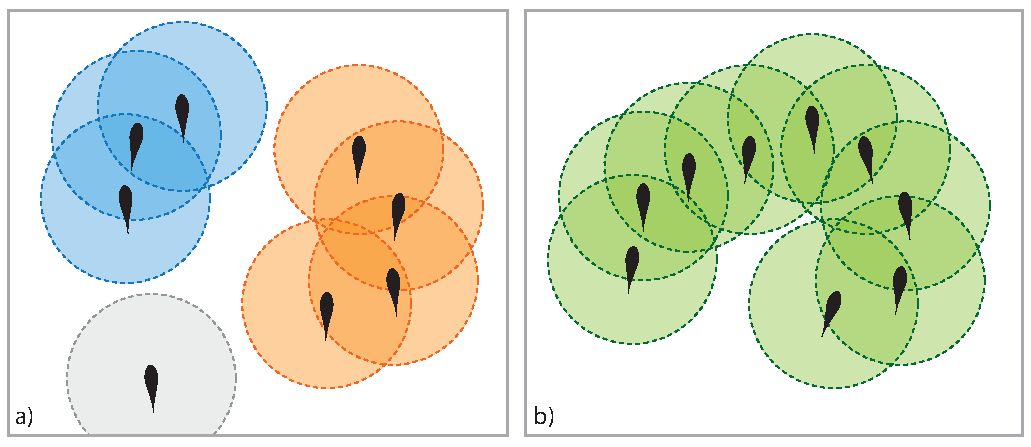
\includegraphics[width=\figurewidth]{scirep/preyGroups}
  \infigurecaption{a) one straggler and two proper groups; the straggler does not see any prey individual from either of the two groups, and no member from one group is able to see neither the straggler nor any prey individual from the other group; potential influence (direct or indirect) is limited to members of the same group only; b) one proper group where all members can potentially (directly or indirectly) influence each other's behaviour.}
  \caption{Prey individuals split into groups based on direct and indirect influence.}
  \label{figure:groups}
\end{figure}

To classify the evolved behaviour we ran five separate simulation runs where on each occasion the artificial world comprised only the prey individuals from the last update step of the corresponding evolutionary run. This was done to preclude the possibility of the behaviour being classified as collective, when in reality all prey are individually trying to escape the predator in a common direction, hence we analysed the evolved behaviour with no predator present. Each simulation run lasted 1800 update steps and on each occasion the type of behaviour was analysed after it reached a dynamically stable state (\ie after 900 update steps). For the analysis we turned to the observation of density \cite{olson2016evolution}, polarization, and angular momentum \cite{couzin2002collective}, properties that allow for the categorization of the type of collective behaviour \cite{couzin2002collective,olson2016evolution,tunstrom2013collective,vicsek2012collective,wood2007evolving}. Density, \eq~\eqref{equation:density}, can be used to assess the degree of grouping, or clumping. Polarization, \eq~\eqref{equation:polarization}, express the degree of consensus in a common heading. Angular momentum, \eq~\eqref{equation:momentum}, the degree of rotation of the group about the group's centre. Together they can be used to assess the type of collective behaviour (\ie swarm, torus, dynamic parallel group, or highly parallel group) \cite{couzin2002collective}. The quantities were recorded over the remaining 900 update steps of a simulation, and their individual averages were used as an indication of the evolved behaviour. 

Normalized prey density
%
\begin{equation}
    \rho_t = \frac{1}{\left|\set{I}\right|^2 - \left|\set{I}\right|} \sum_{i \in \set{I}}{\left|\set{N}^{(i)}_t\right|},\quad \set{N}^{(i)}_t=\{j \in \set{I}|\ j \neq i, \|\vec{r}^{(j)}_t - \vec{r}^{(i)}_t\| \leq r^{(i)}_\textnormal{v}\}
	\label{equation:density}
\end{equation}
%
where $\set{N}^{(i)}_t$ is the neighbourhood of prey individual $i$, was recorded on a global level. However, in view of recent research \cite{viscido2015using}, which emphasizes the importance of calculating the observed quantities on a group-by-group basis, for polarization and angular momentum the prey individuals were first split into groups based on direct and indirect influence (see \figurename~\ref{figure:groups})\cite{lebarbajec2007boids}, where
%
\begin{equation}
\text{1. }\set{G}^{(i)}_t \subseteq \set{I},\quad \text{2. }i \in \set{G}^{(i)}_t,\quad \text{3. if } j \in \set{G}^{(i)}_t \text{ then, } \set{N}^{(j)}_t \subset \set{G}^{(i)}_t, 
\end{equation}
%
is a recursive definition of a group of prey individuals. Prey individuals pertaining to groups of size one, $\sset{S}=\{i \in \set{I}|\ \left|\set{G}^{(i)}_t\right| = 1\}$, are termed stragglers \cite{lebarbajec2007boids} and proper groups can be defined as
%
\begin{equation}
\sset{G}=\{i_1,\ldots,i_n\}:\ \bigcup_{i \in \sset{G} \cup \sset{S}}\set{G}^{(i)}_t = \set{I},\ \forall i,j \in \sset{G}:\ \set{G}^{(i)}_t \cap \set{G}^{(j)}_t = \emptyset.
\end{equation}

Polarization and angular momentum were computed based on proper groups only and in order to diminish the possible bias induced by many small groups the two quantities at time instant $t$ were computed as weighted averages, where group size was used as the weighting function. Hence polarization was computed as
%
\begin{equation}
p_t = \sum_{g \in \sset{G}}{\frac{\left| \set{G}^{(g)}_t\right|p^{(g)}_t}{\left|\cup_{g \in \sset{G}}\set{G^{(g)}_t}\right|}},\quad p^{(g)}_t = \frac{1}{\left|\set{G^{(g)}_t}\right|}{\left\| \sum_{i \in \set{G}^{(g)}_t}{\uvec{v}^{(i)}_t} \right\|},
\label{equation:polarization}
\end{equation}
%
and angular momentum as
%
\begin{equation}
m_t = \sum_{g \in \sset{G}}{\frac{\left| \set{G}^{(g)}_t\right|m^{(g)}_t}{\left|\cup_{g \in \sset{G}}\set{G^{(g)}_t}\right|}},\quad  m^{(g)}_t = \frac{1}{\left|\set{G}^{(g)}_t\right|}{\left\| \sum_{i \in \set{G}^{(g)}_t}{\uvec{r}^{(\set{G},i)}_t \times \uvec{v}^{(i)}_t} \right\|},
\label{equation:momentum}
\end{equation}
%
where $p^{(g)}_t$ and $m^{(g)}_t$ are the polarization and angular momentum of group $g$, respectively and 
%
\begin{equation}
\vec{r}^{(\set{G},i)}_t=\vec{r}^{(i)}_t - \frac{1}{\left|\set{G}^{(i)}_t\right|}\sum_{j \in \set{G}^{(i)}_t}{\vec{r}^{(j)}_t}
\end{equation}
%
is the relative position of prey individual $i$ with respect to the centroid of its group.

%-----
\subsection{Statistical analysis}

The main goal of our experiments (evolution + simulation) was to investigate how the mean of three metrics of interest (normalized prey density, polarization and angular momentum) varies across six different pairs of the four predation tactics (C:H, N:C, P:C, P:H, N:H, P:N) and nine different predation mixtures (8:0, 7:1, ..., 0:8). 

Each combination of the three dimensions above is considered a separate experiment. The experiments are not deterministic -- both the evolution and simulation are stochastic in nature and therefore a source of (random) measurement error. To estimate and account for this, each experiment consisted of $n=20$ different evolutionary runs (iterations), each followed by $m=5$ simulation runs (repetitions). The metrics also vary across individual frames, however, low variability and a relatively high number of frames (900) leads to a negligible standard error, therefore, instead of modelling individual frames, the average across all frames was used.

For each experiment separately, we used the following Bayesian hierarchical model to estimate the mean:
%
\begin{equation}
\begin{split}
y_{ij} &\sim \mathcal{N}(\mu_i, \sigma_i)\\
\mu_{i} &\sim \mathcal{N}(\mu_0, \sigma_0)\\
\mu_0 &\propto 1 \\
\log \sigma_\cdot &\propto 1,
\end{split}
\end{equation}
%
where $y_{ij}$ is the metric measurement for the $j$-th repetition of the $i$-th iteration. That is, we model each iteration with its own distribution with potentially different means $\mu_i$ and standard deviations $\sigma_i$. These means are assumed to be drawn from a population of means, with grand mean $\mu_0$, which is what we are interested in estimating. Flat (improper) priors are placed on the (hyper-)parameters. Note that we are only interested in the mean, so the normal model is adequate, although the data are not normally distributed. 

We used the Stan tool for Bayesian inference to draw samples from the posterior distribution \cite{carpenter2016stan}. Each model was run for 500 warm-up and 5000 sampling iterations, which was sufficient to reduce approximation errors to negligible levels.

In addition to analysing how a specific predation mixture influences the mean of the three metrics (normalized prey density, polarization, angular momentum) we also categorized the behaviour in the last frame (1800) of each simulation run. The categorization was executed on a group-by-group basis following Tunstrøm\etal \cite{tunstrom2013collective}, who defined that a group is in: the polarized state (O) when the group's polarization >\,\num{0.65} and angular momentum <\,\num{0.35}; the milling state (M) when polarization <\,\num{0.35} and angular momentum >\,\num{0.65}; and the swarm state (S) when polarization <\,\num{0.35} and angular momentum <\,\num{0.35}. Outside these ranges it is said to be in transition (T). In addition, a threshold was used to sub-categorize collective states O, M and S as either low <\,\num{0.5} or high density >\,\num{0.5}. The probability of observing a specific collective state was computed by counting the number of groups in that specific collective state over all evolution iterations and simulation run repetitions of an experiment. To diminish the possible bias induced by small groups, each group contributed only a share proportionate to the size of the group. For example, if\ \ $\sset{G}^{(ij)}$ denotes the set of proper groups at the end of iteration $i$, repetition $j$ and $\sset{S}^{(ij)}$ the corresponding subset of proper groups that are in the swarm state, the probability of observing the swarm state was computed as
%
\begin{equation}
P(\textnormal{S}) = \frac{1}{n m}\sum_{i=1}^{n}\sum_{j=1}^{m} \sum_{g \in \sset{S}^{(ij)}}{\frac{\left| \set{G}^{(g)}_{1800}\right|}{\left|\cup_{g \in \sset{G}^{(ij)}}\set{G}^{(g)}_{1800}\right|}}.
\end{equation} 

%-----
\chapterAcknowledgements{The work is part of the PhD thesis that is being prepared by J. Demšar at the Faculty of Computer and Information Science, University of Ljubljana, Slovenia. It was funded in part by the Slovenian Research Agency (ARRS) through the Pervasive Computing research programme (P2-0395). We sincerely thank Janez Demšar for advice on the methods for interpreting results, and Davor Sluga for providing access to computational resources. We would also like to thank Maja Lebar Bajec, Randal S. Olson and Frank H. Heppner for reading and reviewing early versions of this manuscript. Last but not least we would like to thank James Herbert-Read for his assistance with tuning the parameters of our model to biologically relevant values.}

%=====
\begin{subappendices}

%-----
% !TeX root = ./thesis.tex









% this is suplementary information for scirep.tex
%-----
\section{\textsc{Supplementary information:} \textnormal{individual based model}}

The behaviour of the artificial animals -- predators and prey -- in our individual based model is governed by fuzzy logic \cite{zadeh1965fuzzy} via fuzzy-rule-based systems \cite{mamdani1974application}. Every fuzzy-rule-based system is specified via a fuzzy knowledge base, which is made from two parts -- a data base and a rule base. The rule base lists if-then rules that describe the behaviour of the artificial animal in question. The rules are assumed to be joined by the connective ``also,'' so multiple rules can fire simultaneously. The antecedent and consequent parts of individual if-then rules use linguistic terms (near, far, left, right, etc.), which are defined in the data base of the fuzzy-rule-based system. In addition the data base includes information necessary for fuzzy reasoning (see Table~\ref{table:fuzzy}), \ie the method for transforming crisp data into fuzzy sets (fuzzification), the interpretation of logical connectives necessary for fuzzy reasoning, and the method for converting the fuzzy result into a real action (defuzzification). For a detailed description of how a fuzzy rule base is evaluated the reader is invited to refer to \cite{lebarbajec2005fuzzy,lebarbajec2005simulating,mendel2001uncertain}.

\begin{table}
  \caption{Fuzzy data base settings common to predator and prey fuzzy-rule-based systems.}
  \label{table:fuzzy}
  \begin{tabular}{l l}
    \toprule
    Description & Default value \\ [0.5ex]
    \midrule
    Fuzzification & Singleton \\
    Fuzzy conjunction & Product \\
    Fuzzy disjunction & Probabilistic sum \\
    Fuzzy implication & Product \\
    Fuzzy aggregation & Probabilistic sum \\
    Defuzzification & Center of gravity \\
    \bottomrule
  \end{tabular}
\end{table}

In our model, at every update step the fuzzy-rule-based systems (\ie the pre-set fuzzy knowledge base in the case of predators, and the evolving fuzzy knowledge bases in the case of prey individuals) were used to compute the new heading and position of every artificial animal. \tablename~\ref{table:parameters:SM} shows the values of all our model's parameters, while the following sections provide more details about the implementation of the predator and prey artificial animal.

%-----
\subsection{Predators}
The predators in our model were hand-tuned and their behaviour was not subject to evolution. Their fuzzy knowledge base (see \figurename~\ref{figure:predator}) was set as in previous research \cite{demsar2014simulated}, with the only difference being that the predators moved at a constant speed. The fuzzy-rule-based system computed the predator's desired heading direction based on its current target prey individual; it implemented classical pursuit, where the predator moves directly toward the evading target prey individual \cite{kane2014falcons,nahin2012chases}.

\begin{figure}
  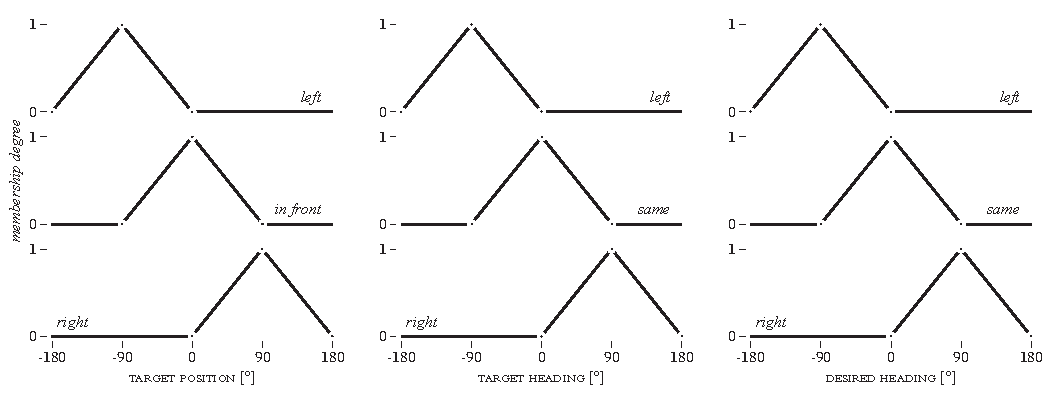
\includegraphics[width=\figurewidth]{scirep/si-predator_db}\\
  \scriptsize
  \vspace*{3mm}
  \begin{minipage}{\figurewidth}
    \textsc{r}1:\quad \textbf{if} (\textsc{target position} \textbf{is} \emph{right}) \textbf{then} (\textsc{desired heading} \textbf{is} \emph{right})\\
    \textsc{r}2:\quad \textbf{if} (\textsc{target position} \textbf{is} \emph{left}) \textbf{then} (\textsc{desired heading} \textbf{is} \emph{left}) \\
    \textsc{r}3:\quad \textbf{if} (\textsc{target position} \textbf{is} \emph{in front}) \textbf{and} (\textsc{target heading} is \emph{right}) \textbf{then} (\textsc{desired heading} \textbf{is} \emph{right})\\
    \textsc{r}4:\quad \textbf{if} (\textsc{target position} \textbf{is} \emph{in front}) \textbf{and} (\textsc{target heading} \textbf{is} \emph{left}) \textbf{then} (\textsc{desired heading} \textbf{is} \emph{left})\\
    \textsc{r}5:\quad \textbf{if} (\textsc{target position} \textbf{is} \emph{in front}) \textbf{and} (\textsc{target heading} \textbf{is} \emph{same}) \textbf{then} (\textsc{desired heading} \textbf{is} \emph{same})
  \end{minipage}
  \caption{The hand-tuned fuzzy knowledge base of the predator fuzzy-rule-based system.}
  \label{figure:predator}
\end{figure}

Let $d^{(i,j)}_t=\|\vec{r}^{(j)}_t-\vec{r}^{(i)}_t\|$ denote the distance between artificial animals $i$ and $j$ at time instant $t$ and $\uvec{d}^{(i,j)}_t=(\vec{r}^{(j)}_t-\vec{r}^{(i)}_t)/d^{(i,j)}_t$ the unit vector pointing from $i$ to $j$ at time instant $t$. The angular position of artificial animal $j$ with respect to $i$ is then
%
\begin{equation}
  \theta^{(i,j)}_t=\arccos\left(\uvec{v}^{(i)}_t \cdot \uvec{d}^{(i,j)}_t\right)
\end{equation}
%
and the relative orientation of artificial animal $j$ with respect to $i$
%
\begin{equation}
  \phi^{(i,j)}_t=\phi^{(j)}_t-\phi^{(i)}_t.
\end{equation}

Let $\kappa$ be a predator and $\alpha$ its current target. To compute the predator's desired heading its fuzzy-rule-based system input variables \textsc{target position} and \textsc{target heading} were set to $\theta^{(\kappa,\alpha)}_t$ and $\phi^{(\kappa,\alpha)}_t$, respectively.

The principal focus of the study was the analysis of the evolved behaviour when varying exposure to multiple simultaneous predation pressures. We used predators that according to previous research might pressure prey towards a) grouping \cite{biswas2014causes,kunz2006prey,olson2013predator,olson2016evolution} (\ie attack the most peripheral prey individual or attack the nearest prey individual) and b) dispersing \cite{olson2013predator} (\ie attack the most central prey individual or attack high density areas).

Let $\set{N}^{(i)}_t=\{j \in \set{I}|\ j \neq i, d^{(i,j)}_t \leq r^{(i)}_\textnormal{v}\}$ denote the neighbourhood of prey individual $i$. High density area attacking predators ($h$) detected and pursued the prey individual with the highest amount of nearby neighbours;
%
\begin{equation}
  \alpha^{(h)}_t = \argmax_{i \in \set{I}} \left|\set{N}^{(i)}_t\right|.
\end{equation}

Note that in the case of a high density area attacking predator (\HDAA predator) the targeted prey individual constantly changed, so that the \HDAA predator effectively detected and pursued the highest density area. Following Olson\etal \cite{olson2013predator} the \HDAA predators moved at a slower speed than prey and were also less manoeuvrable. If the \HDAA predator was close enough to any of the prey individuals (\ie $d^{(h,i)}_t\leq r^{(h)}_\textnormal{c},\ i \in \set{I}$) they were marked as captured. Note also that the \HDAA predator could consume any prey individual and not only the targeted prey individual, therefore mimicking predators capable of attacking and capturing several prey individuals in a single predation event \cite{goldbogen2011mechanics,nottestad1999herring,nottestad2002whales,mori2006first}.

Predators that attack the nearest, the most peripheral or the most central prey individual detect, pursue, attack and capture a single prey individual \cite{demsar2014simulated}. In this study we label them with the common name single-target attack or \ST predators. Note that in contrast to \HDAA predators, in the case of an \ST predator the target prey individual was detected only on special occasions and then pursued until captured or until the predator's hunt duration expired. The detection of the target prey individual occurred at the time instant when the \ST predator appeared or the currently targeted prey individual died during pursuit.

Following previous research \cite{demsar2014simulated,hemelrijk2000towards,hemelrijk2005construction,hildenbrandt2010selforganized}
%
\begin{equation}
  P^{(i)}_t = \frac{1}{\left|\set{N}^{(i)}_t\right|}\left\| \sum_{j \in \set{N}^{(i)}_t} \uvec{d}^{(i,j)}_t \right\|
  \label{equation:peripherality}
\end{equation}
%
is the peripherality of prey individual $i$ at time instant $t$. The peripherality of stragglers, prey individuals with no visible neighbour, \ie $\set{N}^{(i)}_t=\emptyset$, was set to $+\infty$. Let $s$ be an \ST predator. The nearest, $\alpha^{(s)}_\textnormal{n}$, the most peripheral, $\alpha^{(s)}_\textnormal{p}$, and the most central prey individual, $\alpha^{(s)}_\textnormal{c}$, were defined as
%
\begin{equation}
  \alpha^{(s)}_\textnormal{n} = \argmin_{i \in \set{I}} d^{(s,i)}_\sigma,
\end{equation}
%
\begin{equation}
  \alpha^{(s)}_\textnormal{c} = \argmin_{i \in \set{I}} P^{(i)}_\sigma,
\end{equation}
%
\begin{equation}
  \alpha^{(s)}_\textnormal{p} = \argmax_{i \in \set{I}} P^{(i)}_\sigma,
\end{equation}
%
where $\sigma$ is the time instant of target prey individual detection. In view of recent research by Biswas\etal, which suggests that prey clumping emerges regardless of predator confusion \cite{biswas2014causes}, when an \ST predator was close enough to its targeted prey individual (\ie $d^{(s,\alpha)}_t\leq r^{(s)}_\textnormal{c}$, where $\alpha$ is the currently targeted prey) the latter was marked as captured. Meaning that in contrast to previous research \cite{demsar2015simulating,kunz2006prey,olson2013predator,olson2016evolution}, the possibility of the predator getting confused was not explicitly modelled. In other words, predators in our model did not change their target and remained focused throughout the whole hunt event. As a contrast to \HDAA predators, \ST predators were faster than prey, but were also less manoeuvrable.

%-----
\subsection{Prey}

Every prey individual's behaviour was governed by its own fuzzy-rule-based system that, by the application of fuzzy reasoning over an evolving set of if-then rules, determined the individual's desired heading in the next time step. Only the fuzzy rule base was evolved; the fuzzy data base was kept constant (see \figurename~\ref{figure:prey}). The input variables can be decomposed into three parts: a) information regarding the living area, b) information regarding the nearest predator, and c) information regarding the interacting neighbour.

\begin{figure}
  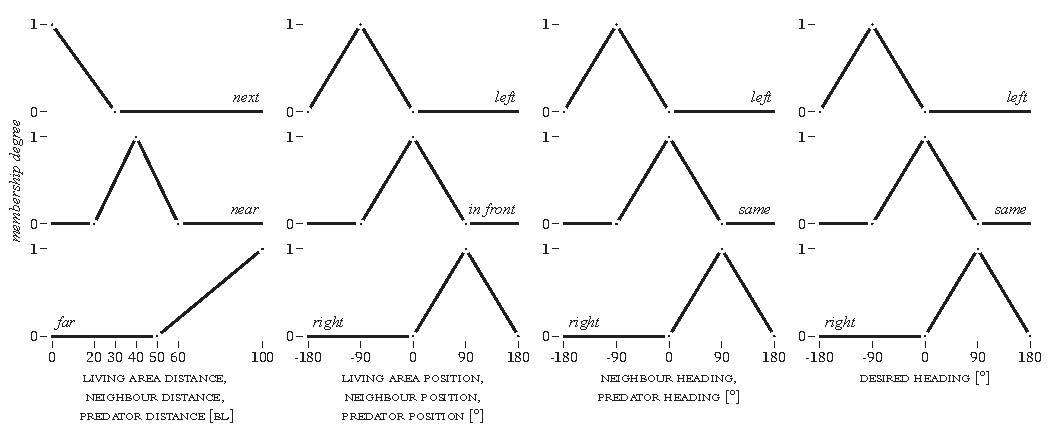
\includegraphics[width=\figurewidth]{scirep/si-prey_db}
  \caption{The data base for prey individuals. The rule base for prey individuals was generated using genetic fuzzy systems.}
  \label{figure:prey}
\end{figure}

At all times prey individuals were aware of the distance and angular position of the nearest point on the border of the living area (\figurename~\ref{figure:preyInput}a), so the input variables \textsc{living area distance} and \textsc{living area position} of prey individual $i$ were set to
%
\begin{equation}
  d^{(i)}_t=\min(0,\ \max(r_\textnormal{LA}-\|\vec{r}^{(i)}_t\|),\ r^{(i)}_\textnormal{v})
\end{equation}
%
and
%
\begin{equation}
  \theta^{(i)}_t=\arccos\left(\uvec{v}^{(i)}_t \cdot \uvec{r}^{(i)}_t\right),
\end{equation}
%
respectively.

\begin{figure}
  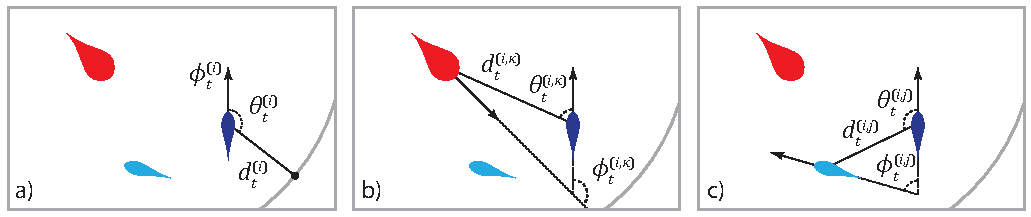
\includegraphics[width=\figurewidth]{scirep/si-interaction}
  \infigurecaption{a) distance, $d^{(i)}_t$, and angular position $\theta^{(i)}_t$ of the nearest point on the border of the living area, b) distance, $d^{(i,\kappa)}_t$, angular position, $\theta^{(i,\kappa)}_t$, and relative orientation, $\phi^{(i,\kappa)}_t$, of the nearest predator, c) distance, $d^{(i,j)}_t$, angular position, $\theta^{(i,j)}_t$, and relative orientation, $\phi^{(i,j)}_t$, of the interacting neighbour.}
  \caption{Quantities available to prey individuals in order to determine their desired heading.}
  \label{figure:preyInput}
\end{figure}

As empirical data suggests that animals in groups usually react to predator attacks\cite{partridge1982structure,pitcher1983predator}, it is safe to assume that in most cases prey individuals can detect the incoming predator attack at some point in time. For this reason, in our model, prey individuals were aware of the nearest visible predator. From the prey individual's point of view this is the predator that poses the highest threat \cite{rieucau2014experimental}. The input variables \textsc{predator distance}, \textsc{predator position}, and \textsc{predator heading} were set to $d^{(i,\kappa)}_t$, $\theta^{(i,\kappa)}_t$, and $\phi^{(i,\kappa)}_t$, respectively (\figurename~\ref{figure:preyInput}b). Here $\kappa$ denotes the nearest currently visible predator of prey individual $i$, computed as
%
\begin{equation}
  \kappa = \argmin_{k \in \set{K}} d^{(i,k)}_t,\ \set{K}=\{k \in \set{S} \cup \set{H}|\ d^{(i,k)}_t \leq r^{(i)}_\textnormal{v}\},
\end{equation}
%
where $\set{K}$ is the set of predators (\ST or \HDAA) currently visible by prey individual $i$. If the prey individual did not see any predators the input variables were marked as \textsc{undefined}. If-then rules with any of their input variables marked as \textsc{undefined} were excluded from fuzzy reasoning.

A large-scale empirical study conducted in Rome \cite{ballerini2008interaction} discovered an anisotropic nature of interactions in starling flocks. This type of interaction became known as topological interaction, where an individual interacts with $\approx$\num{6.5} of its nearest neighbours. Bode\etal \cite{bode2010perceived} proposed a much simpler interaction model capable of replicating the anisotropic nature of the interactions observed in the empirical study. In their model interaction is stochastic in nature and the probability of prey individual $i$ interacting with prey individual $j$ depends on visibility of individual $j$ and is inversely proportional to its distance,
%
\begin{equation}
  p(i,j) = \begin{cases}
    \frac{1}{d^{(i,j)}_t}, &\text{iff }j \in \set{N}^{(i)}_t\\
    0, &\text{otherwise}.
  \end{cases}
  \label{equation:neigbour}
\end{equation}

Following Bode\etal \cite{bode2010perceived} prey individuals in our model at every time instant interacted with only one other prey individual, as this greatly reduces the number of fuzzy-rules that have to be evaluated per prey individual. The fuzzy-rule-based system input variables \textsc{neighbour distance}, \textsc{neighbour position}, and \textsc{neighbour heading} were set to $d^{(i,j)}_t$, $\theta^{(i,j)}_t$, and $\phi^{(i,j)}_t$, respectively (\figurename~\ref{figure:preyInput}c). Like in the case of the input variables related to the nearest predator, if the prey individual had no visible neighbour, i.e $\set{N}^{(i)}_t = \emptyset$ in \eq \eqref{equation:neigbour}, the input variables were marked as \textsc{undefined}.

Evolution was achieved by the application of genetic algorithms over the fuzzy-rule-based systems, \ie by genetic fuzzy systems. Genetic fuzzy systems have been extensively used for the optimization of hand-crafted fuzzy knowledge bases, and evolution of data bases, rule bases or the whole fuzzy knowledge base \cite{cordon2004ten,fernandez2015revisiting,herrera2008genetic}. In our case we pre-specified the data base and used a genetic fuzzy system to evolve only the rule bases of every prey individual. Our inspiration were messy genetic algorithms \cite{goldberg1989messy} which use the Pittsburgh approach: each individual in the population is a complete rule base \cite{hoffman1997evolutionary,smith1980learning}.

\begin{table}
  \caption{Parameters of the genetic fuzzy system.}
  \label{table:ga}
  \begin{tabular}{l l}
    \toprule
    Description & Default (tested) value \\ [0.5ex]
    \midrule
    Number of if-then rules per individual & 2--30 (2--50) \\
    Number of antecedents per rule & 1--2 (1--3) \\
    Mutation rate & 2\% \\
    Mutation intensity & 3 \\
    \bottomrule
  \end{tabular}
\end{table}

The initial population of prey individuals had a randomly generated rule base. The only constraints were the number of if-then rules per individual and the number of antecedents per rule (see \tablename~\ref{table:ga}). The constraints were selected to keep an individual's reasoning as simple as possible. Preliminary tests of the influence of these two constraints on the resulting behaviour by performing evolutions with a higher maximal number of rules (50) and/or antecedents (3) showed results similar to those reported in the main article.

When a prey individual died a new prey individual (child) was created by merging the rule bases of two prey individuals (parents) that were still alive. Selection of parents was fitness proportionate, where the fitness was based on the prey individual's energy level. The number of rules in the rule base of the child prey individual was a uniformly distributed random number between the number of rules in the parent's rule base, whose rule base had the lowest number of rules, and the number of rules in the other parent's rule base. For example, if the rule base of one parent had 15 rules and the other 18 the child could have anywhere between 15 and 18 rules.

Rules in the rule bases of the two parents that had the same antecedent part and the same consequent part of the if-then rule were treated as equal. First equal rules were copied to the child's rule base. Following that the remaining slots were filled with random rules from the set of non-equal rules. Once the child's rule base had the required number of rules there was a 2\% chance a mutation could trigger (mutation rate). There were two kinds of mutations in our genetic fuzzy system; the first type inserted new random rules into the child's rule base, the other removed existing rules. The amount of rules inserted or removed was a uniformly distributed random number between 1 and 3 (mutation intensity). Note that each mutation type could trigger independently so every time a new child prey individual was created each mutation type (insert rules, remove rules) had a 2\% chance of triggering.

%-----
\subsection{Biological relevance of the parameters}

Where possible we attempted to set the model's parameters to biologically relevant values (see \tablename~\ref{table:parameters:SM}). We modelled the prey species after the Pacific Blue-eye (\emph{Pseudomugil signifier}), a fish species that is well known for schooling \cite{herbertread2010sensory,herbertread2015intiation,herbertread2016threedimensional}. In the case of Herbert-Read\etal \cite{herbertread2015intiation} the body lengths (\si{\bodylength}) of captured Pacific Blue-eyes were from \SIrange{2}{3}{\cm}. Other studies \cite{pusey2004freshwater} report an average \si{\bodylength} of approximately \SI{3.5}{\cm}. In our case we used a body length value of \SI{3}{\cm}. The cruising speed of Pacific Blue-eyes is approximately \mps{0.124} $\approx$ \BLps{4} \cite{herbertread2015intiation}. For prey visibility distance we used the equation provided by Tyrell\etal \cite{tyrrell2013looking}. We could not find the exact spatial resolving power of the Pacific Blue-eye so we used the value of a fish of similar size, the zebrafish (\emph{Danio rerio}) \cite{pita2015vision}. This value is relevant since fish of similar size, have similar sized retinas, and thus similar vision capabilities \cite{hairston1982fish}. The zebrafish can spot an object of size \SI{3}{\cm} (the size of a prey individual in our model) at a distance of \SI{330}{\cm}. Because the zebrafish is slightly larger than the Pacific Blue-eye and fish with larger retinas can see farther \cite{hairston1982fish}, we set the visibility distance of prey individuals to \BL{100}. As pointed out by Domenici \cite{domenici2001scaling}, speed changes and body size play a major role in turning rates of fish. Because the speed in our model is constant we could not use the empirical data about fish turning rates. Which is why the maximum manoeuvrability of prey individuals was tuned by hand in such a way that with a hand-tuned fuzzy-rule-based system prey individuals were able to avoid others effectively but without introducing too erratic or jerky movements.

An example of a single-target attack predator that attacks schools of Pacific Blue-eyes is the flathead Gudgeon (\emph{Philypnodon grandiceps}) \cite{herbertread2016threedimensional}. The flathead Gudgeon is usually around \SI{8}{\cm} in length, but it can sometimes grow up to \SI{12}{\cm} in length \cite{pusey2004freshwater}, so we set the size of \ST predators in our model to \BL{3} (\SI{9}{\cm}). The linear regression formula provided by Domenici \cite{domenici2001scaling} suggests that a predator that is 3 times larger than the prey is also approximately \num{1.4} times faster than the prey. Based on that we set the speed of \ST predators in our model to \BLps{5.6}. The \ST predator vision radius calculated using the same approach as for prey individual's \cite{hairston1982fish,pita2015vision,tyrrell2013looking}, would be approximately \BL{300}. However, in mammals \cite{veilleux2014visual}, once the effects of eye size and phylogeny have been statistically controlled, predatory habits are associated with a higher visual acuity. In addition, some aquatic predators, \eg swordfish (\emph{Xiphias gladius}), warm their retina to significantly improve temporal resolution, and hence the detection of rapid motion \cite{fritsches2005warm}. Since the goal of this research is the investigation of behaviour that evolves under various predation pressure mixtures, we wanted to guarantee that the predators can always find and target the most vulnerable prey individual (with respect to the predator's predation tactic). Which is why the vision of predators in our model is not limited. With this we also removed the occurrences when the predator ``did not see a potential prey target.'' To calculate the manoeuvrability of \ST predators we used the equation designed on empirical data by McKenzie\etal \cite{mckenzie2007locomotion}. Using this equation, we calculated that a single target predator should be \num{1.7} times less manoeuvrable than prey.

\begin{table}
  \caption{The individual based model's parameters; \ST -- single-target attack, \HDAA -- high density area attack.}
  \label{table:parameters:SM}
  \renewcommand*{\arraystretch}{.99} % reduce interline spacing by 1%; resolves "Float too large for page by 1.35126pt"
  \begin{tabular}{l l l}
    \toprule
    Parameter & Description & Default value \\
    \midrule
    $\tau$ & Update step & \SI{1}{\second} \\
    $\si{\bodylength}$ & Body length & \SI{3}{\cm} \\
    $r_\textnormal{LA}$ & Living area radius & \BL{350} \\
    \midrule
    $\set{I}$ & Set of prey individuals (size) & 100 \\
    $b^{(i)}$ & Prey appearance area radius & \BL{325} \\
    $s^{(i)}$ & Prey size & \BL{1} \\
    $v^{(i)}$ & Prey speed & \BLps{4} \\
    $r^{(i)}_\textnormal{v}$ & Prey vision radius & \BL{100} \\
    $\omega^{(i)}_\textnormal{max}$ & Prey maximum manoeuvrability &  \rps{0.23}\\
    $\epsilon_0$ & Prey initial energy & \num{1000} \\
    $\epsilon_\textnormal{l}$ & Prey living energy gain & 1 \\
    $\epsilon_\textnormal{c}$ & Prey collision penalty & \num{-10} \\
    $\epsilon_\textnormal{w}$ & Prey wandering penalty & \num{-10} \\
    \midrule
    $t_\textnormal{r}$ & Predator re-appearance time & \SIrange{600}{1200}{\second} \\
    $t_\textnormal{h}$ & Predator hunt duration & \SI{600}{\second} \\
    \hdashline
    $\set{S}$ & Set of \ST predators (size) & 0--8 \\
    $b^{(s)}$ & \ST predator appearance distance & \BL{400} \\
    $s^{(s)}$ & \ST predator size & \BL{3} \\
    $v^{(s)}$ & \ST predator speed & \BLps{5.6} \\
    $r^{(s)}_\textnormal{c}$ & \ST predator catch distance & \BL{3} \\
    $\omega^{(s)}_\textnormal{max}$ & \ST predator maximum manoeuvrability & \rps{0.16} \\
    \hdashline
    $\set{H}$ & Set of \HDAA predators (size) & 0--8 \\
    $b^{(h)}$ & \HDAA predator appearance distance & \BL{400} \\
    $s^{(h)}$ & \HDAA predator size & \BL{12} \\
    $v^{(h)}$ & \HDAA predator speed & \BLps{3} \\
    $r^{(h)}_\textnormal{c}$ & \HDAA predator catch distance & \BL{12} \\
    $\omega^{(h)}_\textnormal{max}$ & \HDAA predator maximum manoeuvrability & \rps{0.03} \\
    \midrule
    $E$ & Duration of evolution & \SI{10000000}{\second} \\
    $I$ & Number of iterations & 20 \\
    \bottomrule
  \end{tabular}
\end{table}

\begin{largefigure} % float too large for page by 16pt [with largefigure environment the max is 37pt]
  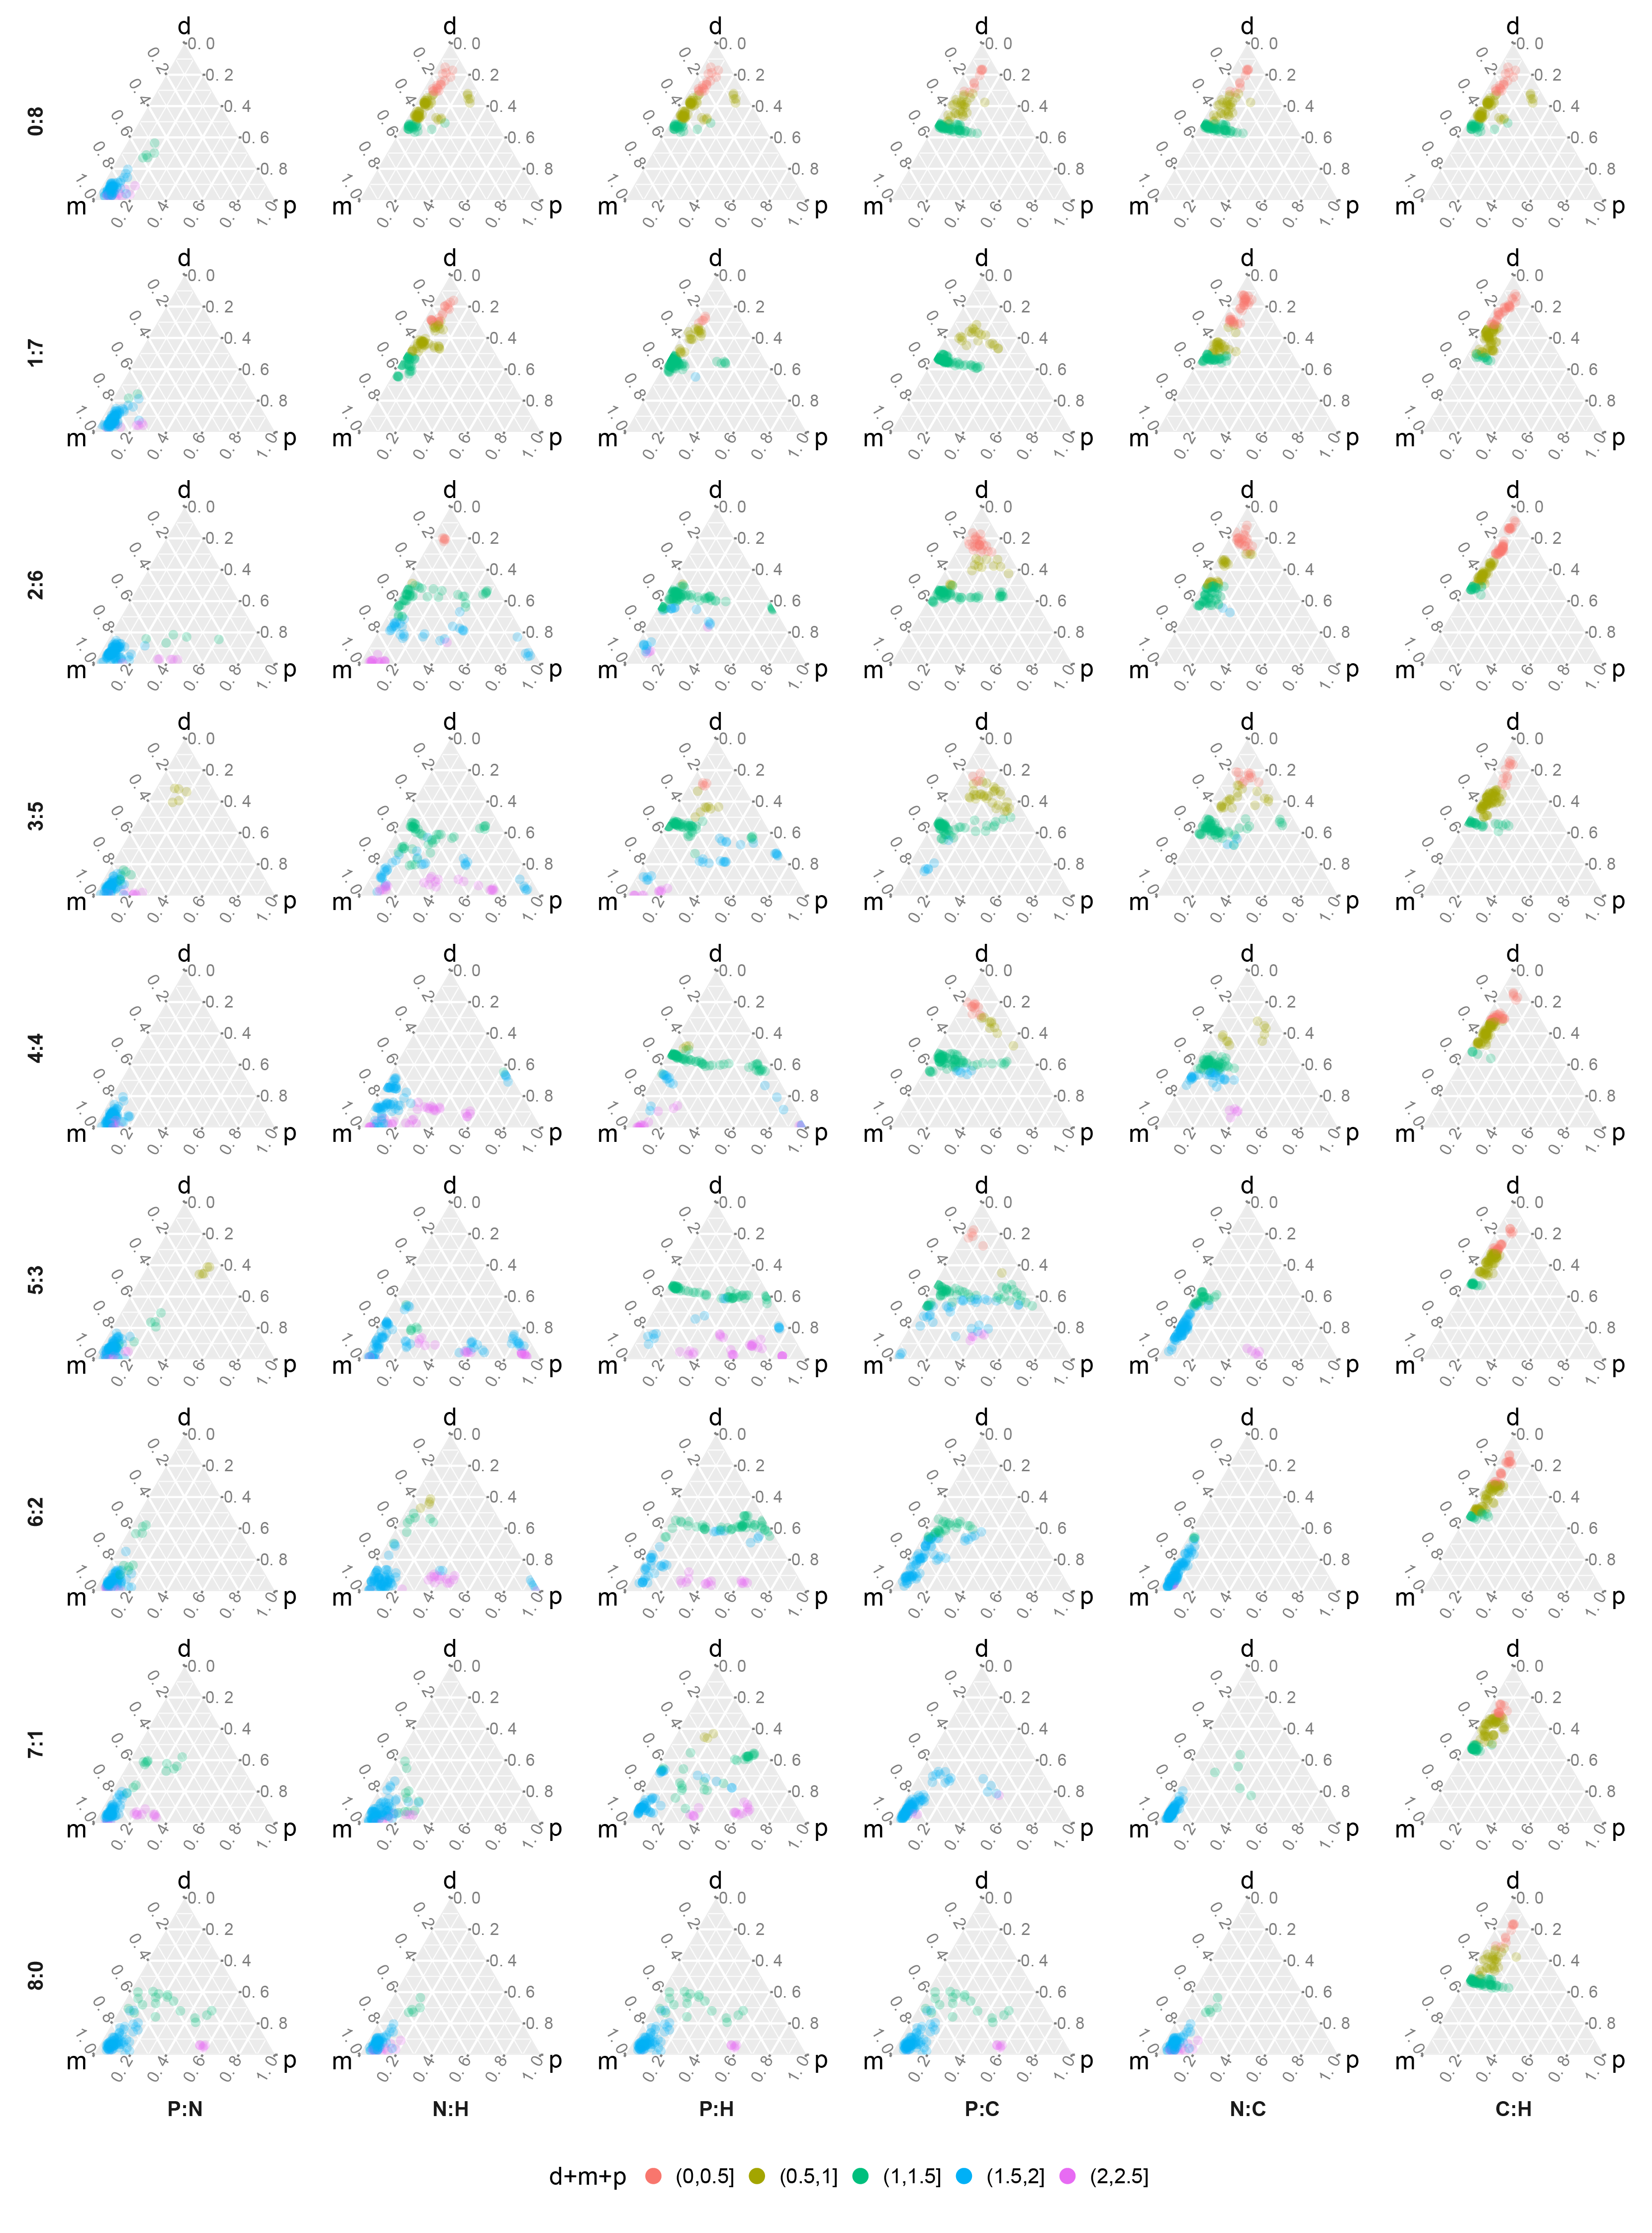
\includegraphics[width=\figurewidth]{scirep/si-tern}
  \infigurecaption{P -- attack prey individuals located at the periphery of the prey groups, N -- attack the nearest prey individual, C -- attack the most central prey individual in a prey group, and H -- high density area attacks. The predator pressure combinations and mixtures were ordered so that the top row and left column, represent the highest pressure towards grouping, the right column and bottom row the highest pressure towards dispersing. The middle section represents antagonistic predation pressures. The scales of the ternary plot were arranged so that the top corner indicates low density, the bottom left corner indicates high density and angular momentum, and the bottom right corner indicates high density and polarization. Note that the ternary plot shows the relationship between the three variables (\ie which one dominates, in relative terms). Since the same point can represent completely different behaviours the sum of the three dimensions is used for colour coding.}
  \caption{Normalized prey density (d), polarization (p) and angular momentum (m) for all predation pressure mixtures, N=\num{5400}.}
  \label{figure:antagonistic:SM}
\end{largefigure}

\begin{video}
  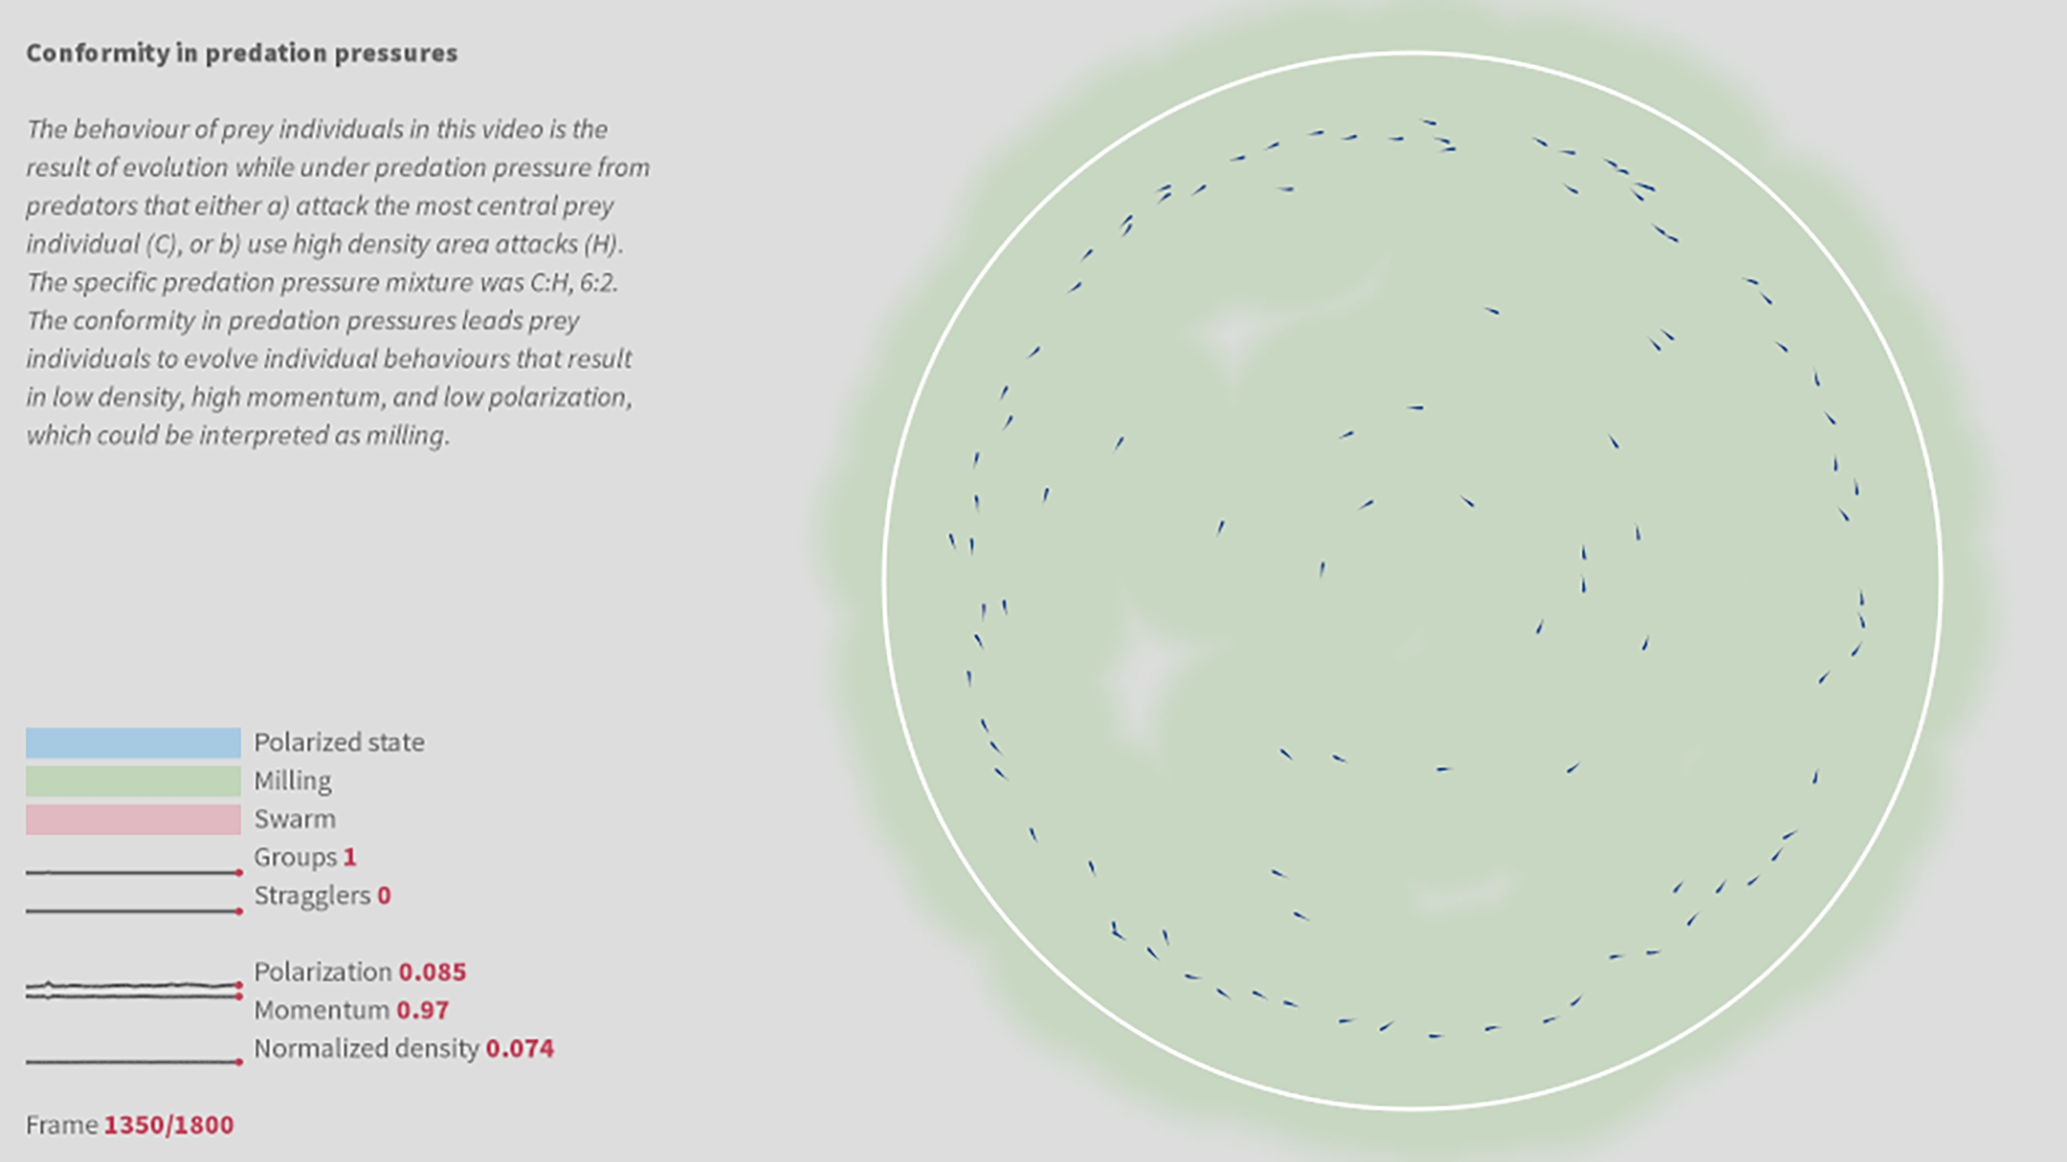
\includegraphics[width=\figurewidth]{scirep/si-V1_1350}
  \infigurecaption{The behaviour of prey individuals in this video is the result of evolution while under predation pressure from predators that either a) attack the most central prey individual (C), or b) use high density area attacks (H). The specific predation pressure mixture was C:H, 6:2. The conformity in predation pressures leads prey individuals to evolve individual behaviours that result in low density, high momentum, and low polarization, which could be interpreted as milling.}
  \caption{Conformity in predation pressures.}
  \label{video:V1}
\end{video}

\begin{video}
  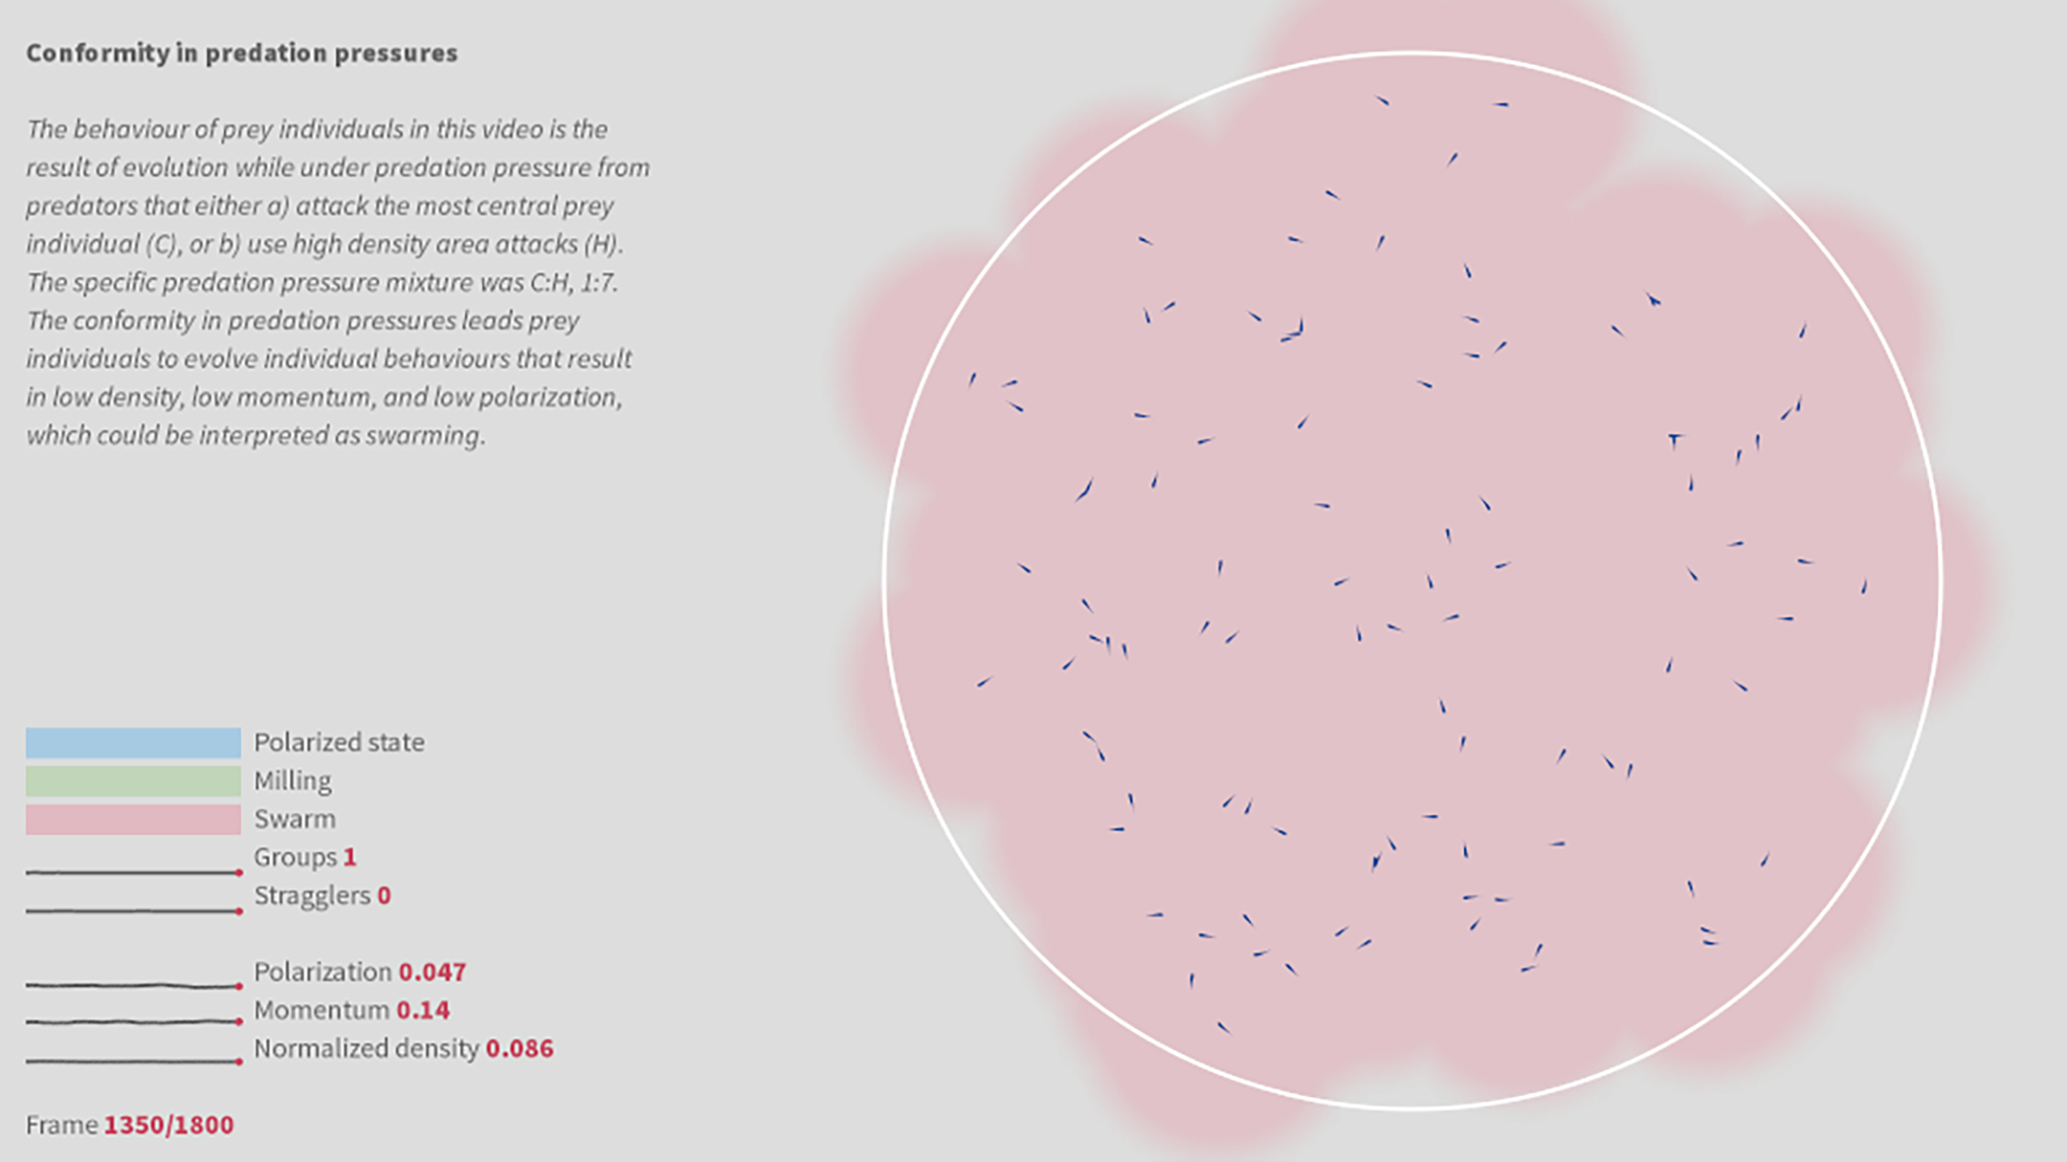
\includegraphics[width=\figurewidth]{scirep/si-V2_1350}
  \infigurecaption{The behaviour of prey individuals in this video is the result of evolution while under predation pressure from predators that either a) attack the most central prey individual (C), or b) use high density area attacks (H). The specific predation pressure mixture was C:H, 1:7. The conformity in predation pressures leads prey individuals to evolve individual behaviours that result in low density, low momentum, and low polarization, which could be interpreted as swarming.}
  \caption{Conformity in predation pressures.}
  \label{video:V2}
\end{video}

\begin{video}
  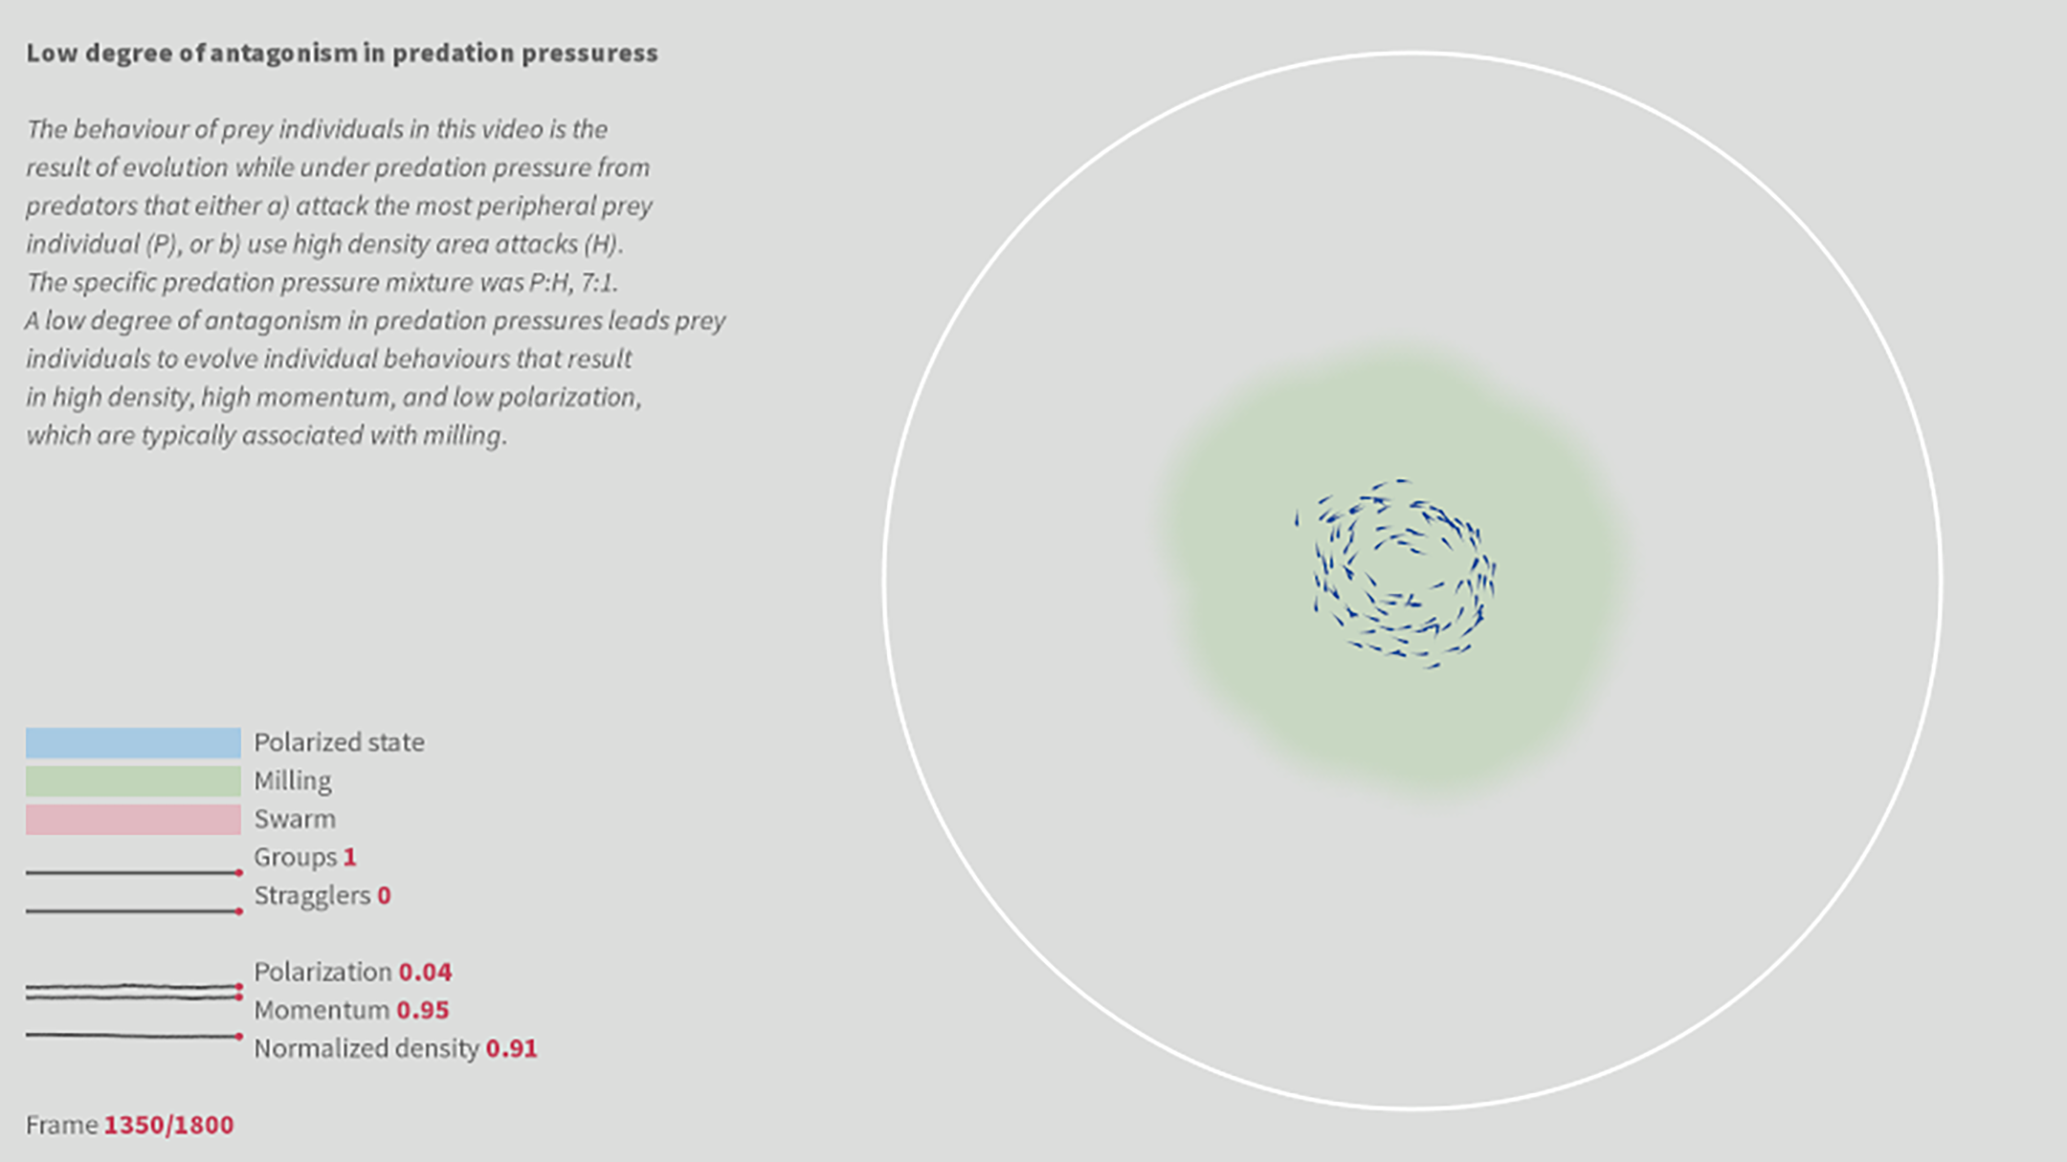
\includegraphics[width=\figurewidth]{scirep/si-V3_1350}
  \infigurecaption{The behaviour of prey individuals in this video is the result of evolution while under predation pressure from predators that either a) attack the most peripheral prey individual (P), or b) use high density area attacks (H). The specific predation pressure mixture was P:H, 7:1. A low degree of antagonism in predation pressures leads prey individuals to evolve individual behaviours that result in high density, high momentum, and low polarization, which are typically associated with milling.}
  \caption{Low degree of antagonism in predation pressures.}
  \label{video:V3}
\end{video}

\begin{video}
  \includegraphics[width=\figurewidth]{scirep/si-V4_1350}
  \infigurecaption{The behaviour of prey individuals in this video is the result of evolution while under predation pressure from predators that either a) attack the most peripheral prey individual (P), or b) use high density area attacks (H). The specific predation pressure mixture was P:H, 7:1. A low degree of antagonism in predation pressures leads prey individuals to evolve individual behaviours that result in high density, low momentum, and low polarization, which are typically associated with swarming.}
  \caption{Low degree of antagonism in predation pressures.}
  \label{video:V4}
\end{video}

\begin{video}
  \includegraphics[width=\figurewidth]{scirep/si-V5_1350}
  \infigurecaption{The behaviour of prey individuals in this video is the result of evolution while under predation pressure from predators that either a) attack the most peripheral prey individual (P), or b) attack the most central prey individual (C). The specific predation pressure mixture was P:C, 5:3. A high degree of antagonism in predation pressures leads prey individuals to evolve individual behaviours that result in medium density, low momentum, and high polarization, which are typically associated with dynamic polarized motion.}
  \caption{High degree of antagonism in predation pressures.}
  \label{video:V5}
\end{video}

\begin{video}
  \includegraphics[width=\figurewidth]{scirep/si-V6_1350}
  \infigurecaption{The behaviour of prey individuals in this video is the result of evolution while under predation pressure from predators that either a) attack the most peripheral prey individual (P), or b) use high density area attacks (H). The specific predation pressure mixture was P:H, 4:4. A high degree of antagonism in predation pressures leads prey individuals to evolve individual behaviours that result in medium density, low momentum, and high polarization, which are typically associated with dynamic polarized motion.}
  \caption{High degree of antagonism in predation pressures.}
  \label{video:V6}
\end{video}

\begin{video}
  \includegraphics[width=\figurewidth]{scirep/si-V7_1350}
  \infigurecaption{The behaviour of prey individuals in this video is the result of evolution while under predation pressure from predators that either a) attack the nearest prey individual (N), or b) use high density area attacks (H). The specific predation pressure mixture was N:H, 5:3. A high degree of antagonism in predation pressures leads prey individuals to evolve individual behaviours that result in high density, low momentum, and high polarization, which are typically associated with highly polarized motion.}
  \caption{High degree of antagonism in predation pressures.}
  \label{video:V7}
\end{video}

 % include suplementary material

\end{subappendices}

	% !TeX root = ./thesis.tex










%==============================
\chapter{Conclusion}
\label{chap:conclusion}

%-----
\EBlettrine{The} phenomenon known as collective animal behaviour is one of the most beautiful spectacles one can observe in nature. Although researched and analysed by scientists from many disciplines and perspectives it is still puzzling in many ways. Examples of such puzzling questions are why did collective behaviour (especially highly organized forms) evolve and why do we see so much variation in behaviour even in closely related species. Through the construction of a genetic fuzzy system capable of evolving various forms of collective behaviour this study represents an attempt in shedding additional light on potential reasons why highly organized collective behaviour evolved.

We started the study by expanding on a known fuzzy model \cite{lebarbajec2005fuzzy,lebarbajec2005simulating} for the purpose of studying predator-prey dynamics in hand-crafted models. Prey animats in this model \cite{demsar2014simulated} could exhibit two types of behaviour -- a social one where they actively strived for grouping (via cohesion and alignment drives) and an individualistic one where they did not. We focused on vision as the principal means of perception, took into account occlusion \cite{kunz2012simulations} and working memory limitations \cite{ballerini2008interaction,engle1999individual,sherry1989hippocampus}, and considered three target selection (predation) tactics. With the first tactic predators attacked the nearest out of visible prey individuals, with the second the most visually isolated prey individual out of the visible ones, and with the third the centre of the visible group (visible prey individuals). To achieve biological relevance we tuned the parameters based on realistic data about birds (starlings, \emph{Sturnus vulgaris}, for prey, and peregrine falcon, \emph{Falco peregrinus}, for the predator). The study suggests that the most successful predator is the one that attacks the most visually isolated individual, while the least successful predator is the one that attacks the centre of the visible group, a result similar to those reported by field observations \cite{zoratto2010aerial}. As a plus, results obtained by our study suggest that, from a prey individual's perspective, social behaviour is more advantageous than individualistic behaviour, which strengthens our belief in the hypothesis that cluster flocking might serve as be a mechanism for protection from predation.

Field observations suggest that predators in nature are able to, at least partially, overcome the defensive benefits of prey grouping by using an assortment of sophisticated hunting strategies \cite{cresswell2011predicting,forsman1998visual,gazda2005division,handegard2012dynamics,hector1986cooperative,kane2014falcons,lopez2006bottlenose,nottestad2002digging,rutz2012predator}. As the parametrization and tuning of such tactics in a hand-crafted model would be a tiresome task we developed an evolutionary model that simulates the evolution of composite target selection tactics \cite{demsar2015simulating}. The most successful predators were those that first dived deep into the centre of the nearby prey group causing chaos and dispersal of the group. Following that they targeted stragglers (individuals that in the process got separated from the rest of the group). The tactic, which we termed as the dispersing tactic, is similar in function to the tactics used by several predators in nature \cite{larsson2012why,pavlov2000patterns}. In our study predators that used the dispersing tactic came out as significantly more successful hunters in a direct competition with predators that used a mixture of simple tactics. Again a result corroborating field observations \cite{pavlov2000patterns}. However, this was true only in the case when our model took into account the possibility of predator confusion. The concept of predator confusion is based on the confusability hypothesis, which suggests that a group of visually similar prey might make it difficult for the predator to select and track its target \cite{nishimura2002predator,zheng2005behavior,kunz2006prey,olson2013predator,olson2016evolution,rutz2012predator}. A different story was the case of the prey's delayed response, a defensive manoeuvre where prey rather then escaping on first sight of the predator, delay their response to a later point in time, and then try to outsmart the predator with rapid movement \cite{partridge1982structure}. The only predators able to, at least to some degree, overcome the defensive benefits of this escape manoeuvre, were again the predators that used the dispersing tactic. Because the dispersing tactic yields higher success to predators we can assume that dispersing the group reduces the group's defensive benefits. This strengthens our belief in the hypothesis that compact groups of prey might function as a defensive mechanism from predation. The absence of an advantage of the dispersing tactic over simple predation tactics when predator confusion is not at play indicates that predator confusion might have played an important role in the evolution of advanced predation tactics, as well. All of these findings were a clear indication of potential interplay between target selection tactics and the evolution of prey group behaviour.

Several studies already pursued the artificial evolution of collective animal behaviour, most by tuning parameters of previously presented non-evolutionary models. Very few succeeded to evolve it from scratch, and even in these cases the evolved behaviour can be termed as ``crude.'' Based on presented material the successful studies portray either clumping \cite{biswas2014causes,hein2015evolution,witkowski2016emergence}, or swarming with collisions \cite{olson2013predator,olson2015exploring,olson2016evolution,witkowski2016emergence}. To study how predation tactics influence the evolution of prey behaviour we designed a novel open-ended, artificial life-like evolutionary model where the drives of individual animats are encoded via linguistic fuzzy rules \cite{demsar2017evolution}. In our genetic fuzzy system prey and predator animats coexist in a shared environment. Based on knowledge about predator target selection tactics gained from our previous research \cite{demsar2014simulated,demsar2015simulating} we designed several types of hand-crafted predators that attack evolving prey. Subsequently, in our model only the survival instincts of prey animats steer the evolution of their behaviour and collective behaviour will emerge only if it will help prey animats survive. We analysed the evolved prey behaviour and showed that based on biologically relevant metrics \cite{couzin2002collective,vicsek2012collective,tunstrom2013collective} our evolutionary model is capable of producing a wide range of behaviours, some qualitatively and visually similar to those reported by experimental studies \cite{tunstrom2013collective}. Since we used a genetic fuzzy system we were able to further analyse the evolved behaviours by studying the fuzzy rule bases that govern the actions of individual animats. Doing so we showed that when clustering the rule bases by the type of evolved behaviour and observing the average proportion of rule antecedents that contain predator related linguistic variables there exists a statistically significant difference between the rule bases. This gives us confidence in advocating that artificial life-like evolutionary modelling based on linguistic fuzzy rule-based systems could be used for answering the illusive biological questions ``why'' collective animal behaviour evolved, and due to their linguistic nature also provide a deeper insight into the ``how.''

To gain further insight into potential ``whys'' we used the newly developed genetic fuzzy system in a controlled experiment where prey evolved while subject to multiple, systematically picked predation tactics simultaneously \cite{demsar2016balanced}. The predation tactics can be split into two groups; those for which the natural defensive response of prey might be grouping and those for which the natural response might be dispersing. We classified the evolved behaviours using quantitative metrics in a similar fashion as previous studies \cite{couzin2002collective,vicsek2012collective,tunstrom2013collective}. When prey evolved while exposed to predators that adopted tactics from only one group the results of evolution corroborated with previous studies \cite{biswas2014causes,olson2013predator,olson2016evolution,wood2007evolving}; prey animats evolved either grouping or dispersing behaviour, with values of metrics characteristic for milling or swarming. When prey animats evolved while exposed to antagonistic pressures that at the same time steered the evolution towards grouping and towards dispersing we detected a significant increase of polarization in motion of prey groups. This suggest that exposure to antagonistic predation pressures might be a necessary requirement for prey individuals to evolve parallel movement. This could indicate that the direction of evolution (grouping or dispersing) is not A versus B, but a labile result -- whether grouping or dispersing evolves depends on a) the nature of the group, and b) the pressures that the group finds itself facing.

\paragraph{Limitations of this study and future work} Throughout our research we devised a number of ideas which could potentially lead to interesting future studies of collective animal behaviour. When it comes to application of evolutionary models for help with providing answers to biological questions the most obvious research advances lie in upgrades towards a higher biological relevance. Evolutionary models are usually simplified due to high computational demands of genetic algorithms and as a result the models are most often restricted to two dimensions, animats in them have unrealistic perception systems, and animats traditionally move with constant speeds, etc. To allow the animats to vary their speed in an evolutionary model we would probably need to implement some kind of fatigue system as well, so that, just like in nature \cite{norin2016measurement,roche2013finding}, animats would not be able to move with their maximum speed indefinitely.

Another possible direction would be the investigation of how heterogeneity influences the evolved behaviour. Some recent studies suggest that in an algorithm mimicking artificial evolution heterogeneous groups might evolve a different behaviour than homogeneous ones \cite{olson2015exploring}. Others suggest that heterogeneous groups might be necessary to achieve a more ``natural'' behaviour \cite{demsar2013family}, and that differences among individuals might be essential for group coordination \cite{marras2012information,marras2013schooling}. In nature heterogeneity (both in behaviour as well as in physiology) is always present, for example birds in a flock often differ in size, gender, age, and some times even species \cite{lebarbajec2009organized,jolles2013heterogeneous}. It is not uncommon that stronger members of the group are positioned at the ``safer'' parts of it \cite{hamilton1971geometry}, which leaves the weaker individuals more exposed to predator attacks. Some predators often intentionally target weak prey individuals \cite{domenici2014howsailfish,marras2015notsofast}, and by using models that consider also physiological heterogeneity one could, apart from studying its influence on prey behaviour, also study how it influences the adaptation of predator target selection tactics.

To our knowledge, in most of the existing models \cite{demsar2014simulated,demsar2015simulating,demsar2016balanced,demsar2017evolution,nishimura2002predator,zheng2005behavior}, the predator animat, once it selects its target, uses classical pursuit \cite{nahin2012chases} to chase its target. In nature some predators use advanced pursuit tactics, for example some species of falcons use the technique of motion camouflage \cite{kane2014falcons}. With this technique they either camouflage themselves against a fixed background object so that the targeted individual observes no relative motion between them and the fixed object, or they approach the targeted individual in a way that, from the targeted individual's point of view the predators always appear to be on the same bearing \cite{justh2006steering}. One possible future study might therefore be a genetic fuzzy system for the evolution of predator pursuit tactics. Or co-evolution of prey behaviour and predator pursuit tactics.

In nature predators often resort to group hunting \cite{creel1995communal,escobedo2014groupsize,fanshawe1993factors,lett2004continuous,muro2011wolfpack,packer1988evolution,scheel1991group}. Occasionally they cooperate (\ie cooperative hunting) to increase the probability of a successful hunting event \cite{creel1995communal,packer1988evolution}. Even though in our current model prey animats are often attacked by several predators at once the predators do not cooperate in any way. Studying the evolution of predator cooperation during hunting events would probably also lead to an interesting study.

Another possible upgrade would be the consideration of short term memory, which comes to play when, for example a predator moves out of view of the targeted individual (out of range or in its blind area). In current models, the targeted individual completely forgets that the predator was attacking it just a moment ago.

An important question is also flight initiation distance. In certain fish species prey as a defence mechanism delay their response \cite{partridge1982structure}. Our research already showed, that a delayed response is quite effective with certain target selection tactics. With an evolutionary model, however, we can study under what conditions (if) such a delayed reaction will emerge. Research in this this direction is already on its way, our current provisional results suggest that the answer might be related to the ratio between predator and prey speed.

The rule base is probably the most important part of a fuzzy animat since it defines the drives of the animat, which have the highest influence on the animat's behaviour. In genetic rule learning the data base of a fuzzy system is static, it does not evolve. As our genetic fuzzy system executes genetic rule learning, fuzzy variables, the linguistic terms, and the interpretation of logic connectives, which are all defined in the data base of a genetic fuzzy systems were hand-crafted. In our research this did not appear to be a limitation as our genetic fuzzy system is capable of evolving many of the forms of collective behaviour that can be commonly observed in nature.

The degree of truth for each fuzzy term is defined by its membership function, these functions come in many shapes (triangular, trapezoidal, singleton, Gaussian, etc.). Even though our algorithm supports many different types of membership functions we developed all models by means of trapezoidal/triangular functions only. These provide the lowest ratio between computational complexity and ease of conceptualization, visualization, and explanation. Again, in the case of our genetic fuzzy system the use of triangular functions did not seem to be a limiting factor as the repertoire of evolved collective behaviours is wider than in previous similar studies \cite{biswas2014causes,hein2015evolution,olson2013predator,olson2015exploring,olson2016evolution,reynolds1993evolved,sayers2009evolved,spector2003emergence,wood2007evolving}. Nevertheless, the evolution of rule bases with more sophisticated types of membership functions and the evolution of the whole fuzzy knowledge base seem like promising research directions for our future work.

To conclude, evolutionary models allowed us to untangle a number of interesting riddles related to collective behaviour already, but judging by the current trends we believe that the best is yet to come.
	\begin{appendices}
	\end{appendices}

\backmatter
	% !TeX root = ./thesis.tex

% use bibtex for bibliography








%==============================
\bibliography{jd}

	% !TeX root = ./thesis.tex










%==============================
\begin{razsirjeniPovzetek}

%-----
\EBlettrine{Ali} imajo jate ptic, jate rib, črede kopitarjev, roji mušic, mehiški val, trume ljudi na koncertu, borza in biološke celice kaj skupnega? S tem se ukvarjajo znanstveniki, ki raziskujejo področje skupinskega vedenja. Primere skupinskega vedenja iz narave prikazuje slika~\ref{fig:CB_si}. Skupinsko vedenje je fascinantno področje, ki analizira, kako preproste odločitve posameznikov vplivajo na dinamiko celotne skupine. Aristotel je nekoč izjavil: »Celota je več kot vsota sestavnih delov.« -- trditev, ki zelo lepo opiše bistvo skupinskega vedenja. Rezultati raziskav iz področja skupinskega vedenja so zanimivi za znanstvenike z več različnih področij, od biologije, fizike in medicine do družboslovnih ved in računalništva \cite{deisboeck2009collective,lebarbajec2009organized,nahin2012chases,silverberg2013collective,spector2003emergence,sumpter2006principles,vicsek1995novel,wei2009pursuit,xu2014crowd}.

\begin{figure}[p]
	\includegraphics[width=\figurewidth]{figCB_BW.png}
	\caption{Primeri različnih režimov skupinskega vedenja, ki jih lahko opazimo v naravi. A) jata škorcev (© Tim Regan, \href{www.flickr.com}{flickr.com}). B) pelikani, ki letijo v formaciji (© Daniel D'Auria, \href{www.flickr.com}{flickr.com}). C) roj kobilic (© FAO emergencies, \href{www.flickr.com}{flickr.com}). D) roj netopirjev (© Amanda, \href{www.flickr.com}{flickr.com}). E) ljudje na koncertu (© Amanda Mustard, \href{http://www.amandamustard.com/}{amandamustard.com/}). F) čreda ovc (© Dariusz Paciorek, \href{http://www.aeroart.com.pl/}{aeroart.com.pl/}). G) ribe v jati, ki ima obliko krogle (© Bo Pardau, \href{www.flickr.com}{flickr.com}). H) kroženje rib okoli praznega jedra (© Robin Hughes, \href{www.flickr.com}{flickr.com}).}
	\label{fig:CB_si}
\end{figure}

Področje skupinskega vedenja (\angl{collective behaviour, collective animal behaviour, swarming behaviour}) je tako zelo aktualno, saj kljub temu, da gre za pojav, ki ga lahko praktično vsak dan srečamo v naravi, mnoga raziskovalna vprašanja ostajajo nerešena \cite{krause2002living,lebarbajec2009organized,sumpter2006principles}. Tako še vedno nismo povsem prepričani, zakaj se nekatere skupine živali (predvsem tiste, kjer se živali gibajo močno usklajeno) pravzaprav sploh tvorijo \cite{lebarbajec2009organized}. Zakaj v naravi obstaja toliko različnih oblik skupinskega vedenja? Zakaj zgolj nekaj vrst ptic, ki letijo v skupinah, to počne v močno usklajenih oblikah? Zakaj so si ptice, ki pripadajo sorodnim vrstam \cite{jarvis2014wholegenome}, po obliki skupinskega vedenja tako različne \cite{lebarbajec2009organized}? V literaturi o skupinskem vedenju lahko najdemo vrsto različnih, tudi nasprotujočih si hipotez o tem, zakaj se živali združujejo v skupine. Nekatere pravijo, da živali tako povečajo učinkovitost pri razmnoževanju in iskanju hrane \cite{krebs1994behavioural}, druge trdijo, da ribe in ptice z usklajenim gibanjem varčujejo z energijo \cite{hemelrijk2014increased,marras2015fish,portugal2014upwash}.

Verjetno najbolj pogosta hipoteza o skupinskem vedenju trdi, da pri živalih združevanje v skupine služi kot učinkovit obrambni mehanizem pred plenilci \cite{cresswell2011predicting,hart2005predator,krause2002living,larsson2012why,lebarbajec2009organized,nishimura2002predator,pavlov2000patterns}. Hipoteza o sebični čredi (\angl{the selfish-herd hypothesis}) trdi, da posamezne živali z združevanjem v skupine zmanjšujejo svoje območje ogroženosti \cite{hamilton1971geometry,viscido2001response}. Hipoteza o zmanjševanju tveganja (\angl{the dilution of risk hypothesis}) razlaga, da ima posameznik manjšo verjetnost, da bo izbran kot tarča plenilca v večjih skupinah \cite{tosh2011conditions}. Hipoteza mnogih oči (\angl{the many eyes hypothesis}) pravi, da se z velikostjo skupine zmanjšuje čas, ki ga mora za odkrivanje nevarnosti vsak posameznik nameniti opazovanju okolice \cite{elgar1989predator,haley2014exploring,ruxton2008application,sadedin1998influence} ter da se z večanjem skupine povečuje verjetnost pravočasne zaznave plenilca \cite{galton1871gregariousness}. Hipoteza o zmedljivosti (\angl{the confusability hypothesis}) predvideva, da ima plenilec težave pri izbiri in sledenju tarče, če se ta nahaja v skupini, ki si je medsebojno vizualno podobna \cite{demsar2015simulating,kunz2006prey,nishimura2002predator,olson2013predator,olson2016evolution,zheng2005behavior}.

Številčnost nekaterih primerkov skupin (na primer jate rib in ptic) je zelo velika in jih težko zapremo v nadzorovano okolje, kjer bi nato znanstveniki lahko preiskovali različne hipoteze o njihovem obnašanju \cite{lebarbajec2009organized}. Obenem v naravi živali prebivajo v različnih okoljih in so podvržene pritiskom različnih plenilcev, ki uporabljalo različne taktike napada. To pomeni, da težko analiziramo zgolj vpliv plenilcev na skupinsko vedenje živali brez posrednega vpliva okolja, v katerem se le-te gibljejo. Računalniški pristopi nam po drugi strani omogočajo razvoj modelov, ki so sposobni reproducirati opazovano vedenje in hkrati odstraniti nezaželene vplive okolja, ki otežujejo empirične raziskave. Prav računalniški pristopi so v zadnjem obdobju vedno bolj pogosti pri raziskovanju raznih hipotez o skupinskem vedenju \cite{vicsek1995novel,couzin2002collective,hildenbrandt2010selforganized}. Ker imajo pri računalniških pristopih znanstveniki popoln nadzor nad vsemi parametri modela, zaključki običajno ne veljajo zgolj za eno samo živalsko vrsto, ampak so lahko tudi bolj splošni.

%-----
\section{Animat}

Eden izmed računalniških pristopov k obravnavi skupinskega vedenja je gradnja modelov, zasnovanih na nivoju posameznika (\angl{individual-based models}). Pri tem pristopu raziskovalci modelirajo lokalni program, ki definira vedenje posamezne simulirane živali (animata, \angl{animat} \cite{cliff1993adding,fine2013unifying,lebarbajec2005fuzzy,watts1998animats,wilson1985knowledge}, slika~\ref{fig:animat_si}), nato pa opazujejo dogajanje pri medsebojni interakciji velikega števila animatov. Običajno je lokalni program, ki definira vedenje posameznika, načrtovan povsem ročno ter se nato skozi čas ne spreminja. To naredi programer/znanstvenik, ki nato v nadaljnjih korakih s spreminjanjem parametrov animata njegovo vedenje priredi do te mere, da slednje čim bolje ponazarja vedenje živali v naravi \cite{couzin2002collective,demsar2014simulated,demsar2015simulating,lebarbajec2005fuzzy,lebarbajec2005simulating,hildenbrandt2010selforganized,vicsek1995novel}. Pri tem si pomaga z različnimi metrikami, ki so jih raziskovalci zabeležili pri empiričnih študijah. Tako načrtovan in pripravljen model se potem s pomočjo izvajanja simulacij nad animati v nadzorovanem umetnem okolju uporabi za različne raziskave skupinskega vedenja. 

\begin{figure}
	\vskip.2in
	\includegraphics[width=.6\figurewidth]{fig_animat_si}
	\vskip.2in
	\caption{Vizualizacija procesov in terminologije povezanih z animatom.}
	\label{fig:animat_si}
\end{figure}

Animat torej povzema osnovne lastnosti pravih živali \cite{lebarbajec2005fuzzy}. Prav tako kot prave živali obstaja v prostoru in času, obkrožajo pa ga živi in neživi objekti, kar pomeni, da animat prebiva v nekem prostoru Animat se zaveda svojega trenutnega stanja in je sposoben zaznavanja stanja bližnje okolice. Ima težnje, ki jih preko izvajanja akcij poskuša zadovoljiti. Tako lahko preko akcij vpliva na svoje stanje ter na stanje prostora.

S pomočjo modelov, zasnovanih na nivoju posameznika, je bilo pokazano, da lahko do zapletenih dinamik skupinskega vedenja pridemo že, če posamezniki sledijo dokaj preprostim težnjam. Prvi poskusi modeliranja skupinskega vedenja s pomočjo modelov zasnovanih na nivoju posameznika segajo v osemdeseta leta prejšnjega stoletja. Aoki \cite{aoki1982simulation} je predlagal pristop od spodaj navzgor za simuliranje jat rib. Reynolds \cite{reynolds1987flocks} je razvil prvi računalniški model za proceduralno animiranje jat ptic. Podobno kot Reynolds sta tudi Heppner in Grenander \cite{heppner1990stochastic} modelirala jate ptic, a s pomočjo stohastičnih nelinearnih diferencialnih enačb. Poleg naštetih modelov se tudi večina novejših \cite{couzin2002collective,demsar2013family,demsar2014simulated,demsar2015simulating,demsar2016balanced,demsar2017evolution,helbing1995social,hildenbrandt2010selforganized,lebarbajec2009organized,parrish2002schools,schellinck2011review,sumpter2006principles,vicsek2012collective} razlikuje zgolj v implementaciji določenega segmenta animata, glavni del, ki definira vedenje, pa je v večini modelov zelo podoben. Vedenje animatov v večini primerov temelji na treh težnjah (Slika~\ref{fig:drives_si}), ki se imenujejo razmik (\angl{separation}), poravnava (\angl{alignment}) in kohezija (\angl{cohesion}). S kohezijo modeliramo težnjo biti blizu drug drugemu. Tako se animat, če nima bližnjih sosedov, želi približati tistim, ki so bolj oddaljeni. S pomočjo težnje razmika animati ohranjajo osebni prostor ter preprečujejo trke. S pomočjo poravnave usklajujejo smer in hitrost gibanja s sosedi. Ker se lahko že zgolj s poravnavo smeri gibanja prepreči razpadanje skupin ter medsebojne trke, nekateri modeli uporabljajo izključno to težnjo \cite{vicsek1995novel}.

\begin{figure*}
	\includegraphics[width=\figurewidth]{figDrives}
	\caption{Vizualizacije treh osnovnih teženj: (a) kohezija, (b) razmik in (c) poravnava. Črni animat je opazovani posameznik. Sivi animati so sosedi, ki neposredno vplivajo na vedenje opazovanega posameznika. Beli animati s sivo obrobo so sosedi, ki nimajo neposrednega vpliva na vedenje opazovanega posameznika.}
	\label{fig:drives_si}
\end{figure*}

%-----
\section{Evolucijski animat}

Nekoliko drugačen pristop predstavljajo modeli, kjer vedenje animatov ni načrtovano povsem ročno, ampak lahko animati svoje vedenje skozi čas spreminjajo samodejno (pri ročno načrtovanih modelih se obnašanje animatov skozi čas ne spreminja). Spremembe vedenja izvajajo za dosego čimbolj učinkovitega zadovoljevanja teženj v danem okolju oziroma prostoru. Običajno so taki modeli osnovani na genetskih algoritmih, ki s pomočjo selekcije, križanja in mutacije posnemajo naravno evolucijo in tako iščejo rešitve za razne kompleksne probleme \cite{goldberg1989genetic,goldberg2002design,holland1992adaptation}. Selekcija zagotavlja, da imajo boljše rešitve oziroma boljši osebki večjo možnost za reprodukcijo. S tem se zagotovi prenos dobrega genetskega materiala v naslednje generacije. Kvaliteta posamezne rešitve se ocenjuje s pomočjo ocenjevalne funkcije. Križanje posnema izmenjavo genetskega materiala pri reprodukciji. Pri formiranju novega osebka se tako kromosomi staršev združijo v en kromosom, ki opredeljuje otroka. S tem se lastnosti staršev prenesejo na otroke. V naravi razne anomalije v reprodukcijskem procesu povzročijo spremembe v genetskem materialu, kar vodi v mutacije, zato genetski algoritmi v zadnjem koraku opravljajo še mutacije -- redke naključne spremembe otrokovega kromosoma. 

Pri najbolj pogosti uporabi genetskih algoritmov so generacije osebkov med seboj običajno povsem ločene. Pred generiranjem nove generacije se najprej oceni kvaliteta vseh rešitev v trenutni generaciji, nato pa se preko izvajanja operacij selekcije, križanja in mutacije ustvari nova enako velika generacija.

V zadnjem času je bilo obljavljenih več pomembnih člankov \cite{kunz2006prey,olson2013predator,olson2016evolution,biswas2014causes,demsar2015simulating,demsar2016balanced,demsar2017evolution,hein2015evolution}, ki so uporabili genetske algoritme za analizo različnih hipotez o evoluciji skupinskega vedenja. Nekateri izmed teh \cite{sayers2009evolved,spector2003emergence,wood2007evolving} so genetske algoritme uporabili predvsem za prilagajanje parametrov v diferencialnih enačbah, ki definirajo znane težnje (težnje izhajajoče iz ne-evolucijskih modelov). Glavna težava pristopa je, da uporaba znanih teženj verjetno usmerja tok evolucije proti razvoju znanega (skupinskega vedenja). Reynolds je bil prvi, ki je uporabil kombinacijo genetskih algoritmov in genetskega programiranja \cite{koza1992genetic} za simuliranje evolucije skupinskega vedenja, ne da bi uporabil vnaprej definirane težnje \cite{reynolds1993evolved}. Vedenje, ki se je v njegovem primeru razvilo, težko primerjamo s kompleksnimi pojavi skupinskega vedenja v naravi. Glavni razlog verjetno tiči v tem, da je bil Reynoldsov model pretirano poenostavljen. Zaera in sod. so pri poskusu simuliranja evolucije skupinskega vedenja uporabili kombinacijo umetnih nevronskih mrež in genetskih algoritmov. Njihov poskus se ni končal najbolje, saj jim ni uspelo razviti vedenja, ki bi bilo podobno primerom iz narave. Po prepričanju avtorjev je glavni razlog za spodletel poskus v ocenjevalni funkciji. Ugotovili so, da je težko definirati ocenjevalno funkcijo, ki dobro opiše pojav skupinskega vedenja s stališča posameznika. Ocenjevalna funkcija je ključni element pri genetskih algoritmih, saj določa, katere rešitve bodo v procesu evolucije vplivale na prihodnje rodove, katere pa bodo izumrle.

Ocenjevanje skupinskega vedenja s stališča posameznika je problematično vsaj z dveh stališč. Definicija stopnje oziroma kvalitete skupinskega vedenja ni najbolj jasna, tako s stališča posameznika kot skupine. V naravi namreč obstaja mnogo različnih režimov skupinskega vedenja. Vsak izmed njih je čudovit in spektakularen na svoj način. Neposredno ocenjevanje stopnje skupinskega vedenja obenem eksplicitno usmerja evolucijo proti razvoju skupinskega vedenja -- posameznike sili k izvajanju akcij, ki povečajo stopnjo skupinskega vedenja. Pri tradicionalni rabi genetskih algoritmov (ko gre za iskanje čim bolj optimalnih rešitev pri kompleksnih nalogah) takšno usmerjanje sicer ni problematično, se pa izkaže kot problematično, ko želimo uporabiti genetske algoritme za raziskovanje možnih vzrokov za razvoj skupinskega vedenja. Pri tovrstnih raziskavah nas bolj kot optimalna znana rešitev zanima, če se bo med animati skupinsko vedenje razvilo samodejno (brez eksplicitnega siljenja s strani ocenjevalne funkcije), kot odgovor na razne zunanje pritiske, ki so prisotni med simulirano evolucijo. 

Vrsta novejših raziskav \cite{biswas2014causes,hein2015evolution,olson2013predator,olson2015exploring,olson2016evolution,witkowski2016emergence} je pokazala, da se skupinsko vedenje razvije tudi z uporabo bolj prikrite ocenjevalne funkcije, in sicer takšne, ki ne usmerja evolucije k razvoju skupinskega vedenja eksplicitno. V omenjenih raziskavah je bila ocenjevalna funkcija zasnovana na sposobnosti preživetja v raznih neugodnih umetnih okoljih. Za preživetje v teh okoljih so animati morali izvajati akcije podobne tistim, ki jih izvajajo živali v naravi -- izmikanje plenilcem, iskanje hrane, itd. Animati, ki so bili pri tem bolj uspešni, so imeli več priložnosti za reprodukcijo. Na ta način so se skozi evolucijo ohranjali zgolj tisti animati, ki so izvajali akcije, s katerimi so uspeli čim več časa preživeti v danem neugodnem okolju. Skupinska vedenja, ki so se v omenjenih raziskavah razvila \cite{biswas2014causes,hein2015evolution,olson2013predator,olson2015exploring,olson2016evolution,witkowski2016emergence}, lahko uvrstimo v dva režima vedenja -- gručenje (\angl{clumping}) in rojenje (\angl{swarming}). V nobeni izmed omenjenih študij se niso razvile usklajene oblike gibanja, ki jih v naravi lahko občudujemo pri jatah rib in ptic -- kroženje okrog praznega jedra (\angl{milling}) oziroma dinamično usklajeno gibanje (\angl{dynamic parallel movement}) \cite{couzin2002collective,sumpter2006principles}.

%-----
\section{Mehki animat}

Najbolj pogosta pristopa za implementacijo animatov sta uporaba diferencialnih enačb \cite{couzin2002collective,hildenbrandt2010selforganized,reynolds1987flocks,vicsek2012collective} ali umetnih nevronskih mrež \cite{kunz2006prey,witkowski2016emergence,zaera1996not}. Umetne nevronske mreže so univerzalni funkcijski aproksimator, ki deluje po vzoru človeških oziroma živalskih možganov. Pristopa sta bila osnova številnih raziskav, ki so pripomogle k večjemu poznavanju skupinskega vedenja. Toda vsak izmed njiju ima določene pomanjkljivosti, ki zavirajo morebiten nadaljnji napredek. Pri diferencialnih enačbah je potrebno podrobno poznavanje vrednosti vseh parametrov modela, za prilagajanje in nadgrajevanje pa potrebujemo dobro matematično znanje. Glavna hiba pristopov, ki uporabljajo umetne nevronske mreže, je težavnost izluščevanja logike delovanja. Hiba je splošno znana in nekateri raziskovalci umetne nevronske mreže posledično označujejo kot pristop s »črno škatlo« \cite{paruelo1997prediction,lek1999artificial,ozesmi1999artificial}.

Lebar Bajec in sod. \cite{lebarbajec2005fuzzy,lebarbajec2005simulating} so za reševanje nekaterih od naštetih težav predlagali uporabo mehke logike (\angl{fuzzy logic}) \cite{zadeh1965fuzzy}. Mehka logika je univerzalni funkcijski aproksimator, tako kot umetne nevronske mreže. Ena izmed glavnih prednosti mehke logike je njena moč, ko operiramo s parametri modela, ki niso povsem natančno znani (so pomanjkljivi, dvoumni, oziroma dvomni). Druga prednost mehke logike je ta, da pri modeliranju uporablja lingvistične opise (če-potem pravila), ki so zelo podobni stavkom, ki jih ljudje tvorimo pri vsakodnevni komunikaciji \cite{kosko1994fuzzy,lebarbajec2005fuzzy,lebarbajec2005simulating,mamdani1975experiment,mendel2001uncertain,zadeh1965fuzzy}. Uporabnost mehke logike za razmeroma preprost prenos opažanj iz narave v modele ter učinkovito modeliranje naravnih pojavov so potrdile že številne raziskave \cite{dasilva2008predator,demsar2013family,demsar2014simulated,demsar2016balanced,demsar2017evolution,lebarbajec2005fuzzy,lebarbajec2005simulating,tron2004mathematical}.

Leta 2005 so Lebar Bajec in sod. predstavili definicijo mehkega animata (\angl{fuzzy animat}) \cite{lebarbajec2005fuzzy,lebarbajec2005simulating}, umetnega živega bitja, zasnovanega s pomočjo mehke logike. Glavna razlika med klasičnim animatom in mehkim animatom je v definiciji pristopa k implementaciji teženj. V primeru klasičnega animata so težnje običajno zapisane v obliki diferencialnih enačb, pri mehkih animatih pa so težnje zapisane v obliki mehkega odločitvenega sistema (\angl{fuzzy rule-based system}). Mehki odločitveni sistem je opredeljen z mehko bazo znanja (\angl{fuzzy knowledge base}), ki je sestavljena iz mehke baze podatkov (\angl{fuzzy data base}) in mehke baze pravil (\angl{fuzzy rule base}). V prvi so deklarirane mehke spremenljivke, mehke vrednosti in interpretacija logičnih povezav. Mehka baza pravil podaja opis obnašanja sistema. V ta namen uporablja lingvistični opis, če-potem pravila v katerih nastopajo logične povezave, mehke spremenljivke in vrednosti. Primer enostavne mehke baze znanja pri sistemu za gretje prostora je predstavljen na sliki~\ref{fig:knowledgebase_si}.

\begin{figure}
	\includegraphics[width=\figurewidth]{figKnowledgebase_si}
	\caption{Primer enostavne mehke baze znanja. Primer prikazuje mehki sistem za gretje prostora. Zgornji del vizualizira mehko bazo podatkov, definirani imamo dve mehki spremenljivki -- eno vhodno in eno izhodno. Vhodna spremenljivka je trenutna temperatura v prostoru, ki jo sistem pridobi s pomočjo senzorja za temperaturo. Mehka baza pravil (spodnji del) opisuje, kako se vhodne spremenljivke pretvorijo v akcije (izhodne spremenljivke) preko če-potem pravil. V našem primeru je akcija sistema za gretje sprememba v temperaturi prostora.}
	\label{fig:knowledgebase_si}
\end{figure}

V primeru animatov mehka baza podatkov definira, kako animati interpretirajo svojo okolico oziroma informacije, ki jih dobijo iz okolice s pomočjo zaznavanja (na primer razdaljo do najbližjega soseda, smer gibanja plenilca, položaj ovire, itd.) ter definira akcije, ki jih lahko izvajajo za spremembo lastnega stanja in/ali stanja prostora (na primer spremembo hitrosti, spremembo smeri gibanjam itd.). Kako mehki animat pretvori pridobljene informacije v akcije je definirano v mehki bazi pravil.

%-----
\section{Cilj: evolucijski mehki animat}

Glavni cilj pričujoče disertacije je bil razvoj umetnega genetskega sistema, primernega za simuliranje evolucije pojavov skupinskega vedenja s pomočjo mehke logike. Ker najbolj pogosta hipoteza o nastankih skupinskega vedenja trdi, da se je pojav morda razvil kot zaščita pred plenilci \cite{cresswell2011predicting,hart2005predator,krause2002living,larsson2012why,lebarbajec2009organized,nishimura2002predator,pavlov2000patterns}, lahko predpostavimo, da je boj za preživetje med plenilci in plenom verjetno smiseln del evolucijskega modela. Da bi pri konstrukciji in validaciji evolucijskega modela naleteli na čim manj težav, smo se odločili, da bomo najprej preučili dinamiko med plenilci in plenom v ročno načrtovanem modelu. S pomočjo analize taktik napada v ročno načrtovanem modelu \cite{demsar2014simulated} smo pridobili tako znanje o taktikah napada, ki jih uporabljajo plenilci, kot tudi vpogled v reakcije plena ob napadu plenilca. Med študijo smo spoznali, da plenilci v računalniških modelih večinoma uporabljajo zgolj osnovne taktike napada. Po drugi strani pa plenilci, ki v naravi napadajo plen, ki se zadržuje v skupinah, uporabljajo različne in pogostokrat zelo izdelane taktike napada. Zato smo v naslednjem koraku razvili evolucijski model, v katerem plenilci prilagajajo taktike napada s ciljem doseganja čim višje uspešnosti pri lovu. Z raziskavo smo skušali dobiti odgovor na vprašanje o optimalni taktiki napada v odvisnosti od režima skupinskega vedenja oziroma odziva plena \cite{demsar2015simulating}.

S pomočjo znanja, pridobljenega v okviru teh dveh raziskav, smo nato razvili umetni genetski mehki sistem (\angl{genetic fuzzy system}), ki je primeren za simuliranje evolucije skupinskega vedenja. Genetski mehki sistemi \cite{cordon2001genetic,cordon2004ten,fernandez2015revisiting,herrera1996genetic,herrera2008genetic,pedrycz1996fuzzy,sanchez1997genetic} izkoriščajo genetske algoritme za optimizacijo ali konstrukcijo mehkih baz znanja. Večina genetskih mehkih sistemov se ukvarja z optimizacijo ročno načrtovanih mehkih sistemov \cite{cordon2004ten,fernandez2015revisiting,herrera2008genetic}. Zahtevnejši pristop je genetsko učenje mehkih sistemov (\angl{genetic learning of fuzzy systems}), pri katerem se genetski algoritmi ne uporabljajo zgolj za optimizacijo obstoječih mehkih sistemov, ampak se komponente sistema (mehko bazo znanja, mehko bazo podatkov, ali mehko bazo pravil) ustvari kar s pomočjo genetskih algoritmov. V tej disertaciji se osredotočamo na ustvarjanje mehkih baz pravil (tudi genetsko učenje pravil) animatov. Pri animatih je mehka baza pravil verjetno najbolj pomemben del mehkega sistema, saj je v njej zapisano kako animat zaznane informacije pretvori v akcije.

V literaturi lahko najdemo dva prevladujoča pristopa k genetskemu učenju pravil -- michiganski pristop \cite{holland1977cognitive} in pittsburški \cite{smith1980learning} pristop. Pri prvem kromosom v genetskem algoritmu predstavlja posamezno pravilo, kar pomeni, da celotna generacija predstavlja eno samo mehko bazo pravil. Kvaliteta (ocena) mehke baze pravil (ustreznost za reševanje danega problema) torej narašča skozi povsem ločene generacije. V našem primeru bi to pomenilo, da je vsem animatom dodeljena identična baza pravil. Ker tega nismo želeli, smo se odločili za uporabo pittsburškega pristopa. Pri tem posamezen kromosom predstavlja celotno mehko bazo pravil. Na tak način smo lahko vsak animat obravnavali kot posameznika (vsak animat je definiran s svojim kromosomom). S tem smo se tudi odmaknili od klasične uporabe genetskih algoritmov, kjer so generacije med seboj povsem ločene in se približali simuliranju umetnega življenja (\angl{artificial life}), kjer ni povsem jasnih medgeneracijskih mej -- selekcija, križanje in mutacija so del odvijajoče se evolucije. Ker je v našem sistemu vsak animat definiran s svojim kromosomom, je rezultat heterogena populacija animatov (heterogena po obnašanju in ne po fiziologiji). Tako bi lahko rekli, da se animati, preko svojih mehkih baz pravil, borijo za preživetje v okolju, ki je tekmovalno iz dveh pogledov. Prvi del boja za preživetje animati bijejo s plenilci, drugi del pa med seboj, ko si poskušajo izboriti večjo možnost za reprodukcijo. S tem pristopom ter z uporabo različnih taktik napada pri plenilcih nam je uspelo razviti mehki genetski sistem, ki je sposoben generirati večji nabor režimov skupinskega vedenja \cite{demsar2017evolution}, kot so jih sposobne reproducirati obstoječe raziskave \cite{biswas2014causes,hein2015evolution,olson2013predator,olson2015exploring,olson2016evolution,reynolds1993evolved,sayers2009evolved,spector2003emergence,wood2007evolving}. Sistem smo nato v nadaljevanju uporabili za analizo vpliva različnih sočasnih pritiskov na obliko skupinskega vedenja, ki nastane ob evoluciji \cite{demsar2016balanced}.

%-----
\section{Rezultati}

V prvi fazi raziskav smo razvili nov mehki model \cite{demsar2014simulated} za simulacijo letenja ptic v jati, ko so te izpostavljene napadom plenilca. Interakcija v modelu in taktike napada temeljijo na vizualni zaznavi. Pri tem upoštevajo prekrivanje oddaljenih predmetov s strani bližnjih \cite{kunz2012simulations} in omejitve delovnega spomina \cite{ballerini2008interaction,engle1999individual,sherry1989hippocampus}. Taktike napada plenilca so bile tri -- napad najbližjega izmed vidnih animatov, napad najbolj vizualno ločenega izmed vidnih animatov in sredine skupine vidnih animatov. V raziskavi smo obravnavali dva režima vedenja plena, in sicer socialno, kjer se animati z upoštevanjem nagonov kohezije in poravnave aktivno združujejo v jate in individualno, kjer tega ne počnejo (izogibajo se zgolj trkom). Rezultati kažejo, da je najbolj uspešen plenilec tisti, ki lovi vizualno ločene osebke, a to predvsem v primerih, ko je vedenje plena socialno. Ko je vedenje plena individualno, je s stališča plenilca najboljša taktika napad najbližjega. S stališča plena je socialno vedenje boljše, saj ne glede na taktiko napada plenilca podaljša čas, ki ga slednji potrebuje za ulov. To krepi hipotezo, da se je združevanje v skupine lahko razvilo kot zaščita pred plenilci. Obenem pa nakazuje, da je najboljša taktika plenilca močno odvisna od vedenja plena.

V drugi fazi smo nato razvili evolucijski model \cite{demsar2015simulating}, v katerem smo s pomočjo genetskih algoritmov prilagajali parametre, s katerimi so bile definirane ročno načrtovane taktike napada. S pomočjo prilagajanja parametrov taktik se je plenilcem skozi čas povečala uspešnost pri lovu. Z namenom lažje primerljivosti z ostalimi raziskavami smo se osredotočili na znane osnovne taktike napada (napad najbližjega, napad najbolj izoliranega in napad najbolj središčnega animata, ki predstavlja plen), a tem dodali še napredno dvofazno taktiko. S to taktiko, ki smo jo poimenovali razpršilna (\angl{dispersing}), se plenilec najprej usmeri v središče jate, da bi v njej povzročil kaos in njen razkroj, nato pa se osredotoči na najbolj izolirane posameznike. Taktiko uporablja več vrst plenilcev v naravi \cite{larsson2012why,pavlov2000patterns}. V raziskavi smo nato obravnavali tako vpliv zmedljivosti plenilca, kot tudi kaj se zgodi, če plen, ki se združuje v jate, kot obrambni mehanizem izvaja manever zakasnjenega odziva, kjer se na napad ne odzove ob prvi zaznavi plenilca, ampak odziv zakasni. Rezultati kažejo, da je razpršilna taktika najuspešnejša in edina sposobna vsaj v določeni meri izničiti uspešnost zakasnjenega odziva kot obrambne taktike plena. Ker je uspešnost plenilca s prilagajanjem razpršilne taktike bistveno upadla, če ta ni bil zmedljiv, slednje nakazuje, da je zmedljivost lahko igrala pomembno vlogo v evoluciji naprednih taktik napada.

Glede na znanje pridobljeno s predhodnimi fazami raziskave smo z namenom evolucije skupinskega vedenja v tretji fazi razvili genetski mehki sistem \cite{demsar2017evolution}, ki temelji na umetnem življenju. Animati, ki predstavljajo plen, so se razvijali pod sočasnimi pritiski plenilcev, ki uporabljajo več ročno načrtovanih taktik napada (napad najbližjega posameznika, napad najbolj izoliranega posameznika, napad najbolj središčnega posameznika in napad najgostejšega predela skupine). S prvimi tremi taktikami plenilec lovi in ujame zgolj enega samega posameznika, pri zadnji pa plenilec lahko lovi in ujame več posameznikov hkrati (kot to v naravi počno nekatere vrste morskih kitov \cite{domenici2001scaling,goldbogen2011mechanics,nottestad1999herring,nottestad2002whales}). Ker so animati, ki predstavljajo plen, sobivali v okolju s plenilci, pri čemer je bil cilj prvih preživeti, drugih pa ujeti čim več posameznikov, je nastanek skupinskega vedenja pogojen zgolj s tem, da animatom v tem okolju pomaga preživeti čim dlje. Rezultati kažejo, da model razvije večje število režimov skupinskega vedenja, kot obstoječe raziskave \cite{biswas2014causes,hein2015evolution,olson2013predator,olson2015exploring,olson2016evolution,reynolds1993evolved,sayers2009evolved,spector2003emergence,wood2007evolving}. Analiza mehkih pravil je pokazala, da se režimi vedenja statistično značilno razlikujejo po deležu pravil, ki upoštevajo plenilca.

V četrti fazi raziskav smo zato izvedli kontroliran eksperiment evolucije, kjer smo sistematično izbirali taktike napada, katerim so bili animati med evolucijo izpostavljeni \cite{demsar2016balanced}. Osredotočili smo se na to, kako različni pritiski vplivajo na režim skupinskega vedenja, ki se razvije. Rezultati potrjujejo dotedanje raziskave \cite{biswas2014causes,olson2013predator,olson2016evolution,wood2007evolving}, da se a) v primeru taktik napada na najbližjega oz. najbolj izoliranega posameznika razvije združevanje v skupine, ter da se b) v primeru taktik napada na najbolj središčnega posameznika oz. najgostejši del jate razvije razprševanje. V teh primerih so se razvile oblike gibanja, ki so najbolj podobne rojenju oziroma kroženju okrog praznega jedra. Najbolj zanimivi rezultati so nastali v primerih, ko so bili animati izpostavljeni taktikam, od katerih nekatere usmerjajo evolucijo plena k združevanju v skupine, nekatere pa k razpršitvi. Zgolj v teh primerih so se namreč razvile usklajene oblike gibanja, ki jih v naravi občudujemo v jatah ptic in rib (dinamično usklajeno gibanje in močno usklajeno gibanje).

Vsaka izmed faz predstavlja lasten izviren doprinos k znanosti in vsaka je bila predstavljena v svojem izvirnem znanstvenem prispevku \cite{demsar2014simulated,demsar2015simulating,demsar2017evolution,demsar2016balanced}.

%-----
\section{Nadaljne raziskave}

V procesu raziskav, predstavljenih v pričujoči disertaciji, se nam je porodilo več idej, ki bi lahko bile potencialno zanimive za nadaljnje raziskave skupinskega vedenja. Pri uporabi evolucijskih modelov za iskanje odgovora na biološka vprašanja so verjetno trenutno največja hiba poenostavitve modelov, ki se jih raziskovalci poslužujejo zaradi velike računske zahtevnosti tako genetskih algoritmov, kot že samih računalniških modelov skupinskega vedenja. Za zvišanje biološke relevantnosti evolucijskih modelov bi bilo dobro odstraniti čim več poenostavitev. Med najbolj pogoste sodijo omejitev gibanja animatov na dve dimenziji, nerealistični sistemi zaznavanja, gibanje s konstanto hitrostjo, itd. Če na primer hočemo animatom v evolucijskih modelih omogočiti spreminjanje hitrosti, bo verjetno potrebno najprej implementirati porabo energije, ki bo posledično vodila v to, da se animati lahko tudi utrudijo. S tem se animati, prav tako kot živa bitja v naravi \cite{norin2016measurement,roche2013finding}, ne bi mogli ves čas premikati z maksimalno hitrostjo, ki jo lahko dosežejo. 

Ena izmed možnih smeri nadaljnih raziskav bi lahko bila tudi analiza vpliva heterogenosti v fiziologiji na evolucijo skupinskega vedenja. Nekatere aktualne raziskave namigujejo, da heterogene skupine v evolucijskem modelu razvijejo drugačno vedenje, kot homogene \cite{olson2015exploring}. Druge nakazujejo, da je heterogenost morda pomembna za dosego bolj ``naravnega'' vedenja \cite{demsar2013family} in da so morda razlike med posamezniki pomembne za koordinacijo skupine \cite{marras2012information,marras2013schooling}. V naravi je heterogenost (tako v vedenju kot v fiziologiji) vedno prisotna. Na primer ptice se v jatah pogosto razlikujejo v velikosti, spolu, starosti in včasih celo v vrsti \cite{lebarbajec2009organized,jolles2013heterogeneous}. Tako pogosto vidimo, da se močnejši posamezniki nahajajo v najbolj varnih predelih skupine \cite{hamilton1971geometry}, posledično pa so šibkejši posamezniki bolj izpostavljeni napadom plenilcev. Nekateri plenilci v naravi celo namenoma napadajo šibkejše posameznike \cite{domenici2014howsailfish,marras2015notsofast}. Z razvojem modela, v katerem bi bili animati heterogeni tudi po fiziologiji, bi lahko, poleg vpliva heterogenosti na evolucijo skupinskega vedenja, analizirali tudi to, kako plenilci prilagodijo svoje taktike napada pri napadu heterogenih skupin.

V večini obstoječih modelov \cite{demsar2014simulated,demsar2015simulating,demsar2016balanced,demsar2017evolution,nishimura2002predator,zheng2005behavior} plenilec za sledenje izbrani tarči uporablja tehniko klasičnega zasledovanja (\angl{classical pursuit}) \cite{nahin2012chases}. V naravi najdemo tudi plenilce, ki uporabljajo bolj napredne tehnike sledenja tarči. Nekatere vrste sokolov uporabljajo tehnike sledenja, s katerimi zakrivajo svojo smer gibanja (\angl{motion camouflage}) \cite{kane2014falcons}. To dosežejo na več načinov. Tarčo lahko pretentajo s pomočjo objektov v ozadju, ali pa se ji približujejo pod takim kotom, da tarča tega približevanja ne opazi \cite{justh2006steering}. Tako bi lahko s pomočjo genetskih algoritmov poleg taktik napada razvijali tudi taktike sledenja, ali pa bi celo sočasno razvijali skupinsko vedenje in taktike sledenja plenilcev. Na njihovo soodvisnost so opozorile že naše uvodne raziskave.

V naravi pogosto lahko opazimo tudi pojav skupinskega lova \cite{creel1995communal,escobedo2014groupsize,fanshawe1993factors,lett2004continuous,muro2011wolfpack,packer1988evolution,scheel1991group}. Pri skupinskem lovu več plenilcev sodeluje med sabo in si s tem izboljša možnosti za uspešen ulov. Čeprav je v naših modelih lahko sočasno aktivnih več plenilcev, le-ti ne sodelujejo med sabo. Analiza evolucije sodelovanja plenilcev med lovom bi verjetno privedla do zanimive raziskave in rezultatov.

Nenazadnje, eno izmed pomembnih vprašanj je, kdaj se bo plen po zaznavi napada odločil začeti bežati. V naravi nekatere vrste rib kot obrambni mehanizem namensko zakasnijo odziv \cite{partridge1982structure}. Naše raziskave so že nakazale, da je omenjeni manever pri določenih taktikah napada uspešen. Evolucijski model pa omogoča pridobiti odgovore na vprašanje pod kakšnimi pogoji se tak zakasnjen odziv razvije. Raziskave v tej smeri že izvajamo in trenutni rezultati nakazujejo, da se odgovor morda navezuje na razmerja v hitrostih med plenilcem in plenom.

S pomočjo evolucijskih modelov smo razvozlali že marsikatero uganko glede skupinskega vedenja, glede na trenutne smernice pa verjamemo, da najzanimivejši odgovori šele prihajajo.

\end{razsirjeniPovzetek}

\end{document}
